%%% VCU thesis/dissertation template file
\makeatletter
\let\my@xfloat\@xfloat
\makeatother

\documentclass[reqno]{vcuthesis}
\makeatletter
\def\@xfloat#1[#2]{
        \my@xfloat#1[#2]%
        \def\baselinestretch{1}%
        \@normalsize \normalsize
}
\makeatother
%%%%%%%%%%%%
% PACKAGES %
\usepackage{bm,amsmath,subfigure,graphicx,url,algorithm,algorithmicx,algpseudocode,booktabs}
\usepackage{tikz-cd,adjustbox,amsfonts,mathtools,tabularx,capt-of,longtable,comment,caption,soul}
\usepackage[flushleft]{threeparttable}
\usepackage[top=1in,bottom=1in,right=1in,left=1in]{geometry}
\usepackage[backend=bibtex]{biblatex}
\usepackage[titletoc]{appendix}
\usepackage{pgfplots}
\pgfplotsset{compat=1.12}
\usepackage[linktocpage=true]{hyperref}
\usetikzlibrary{shapes.geometric,arrows,automata,positioning}
\usepackage{chngcntr}
\usepackage[final]{pdfpages}
\usepackage[explicit]{titlesec}

\newcommand{\iitem}{\item[-]}
\newcommand{\set}[1]{{\left\{#1\right\}}} 
\newcommand{\norm}[1]{{||#1||}} 
\renewcommand{\st}{{\,|\,}} 
\newcommand{\reals}{{\mathbb{R}}}
\newcommand{\ints}{{\mathbb Z}}
\newcommand{\spa}[1]{\mathcal{#1}}
\newcommand\tab[1][1cm]{\hspace*{#1}}
\newcommand{\Rho}{\mathrm{P}}
\newcommand{\proc}{{\mathcal P}}
\newcommand{\tup}[1]{\left(#1\right)}

\def\checkmark{\tikz\fill[scale=0.4](0,.35) -- (.25,0) -- (1,.7) -- (.25,.15) -- cycle;} 

%%%%%%%%%%%
\overfullrule=5pt
% BIBLIOGRAPHY %
\bibliography{references}
\renewcommand{\type}{Dissertation}
\renewcommand{\thetable}{\arabic{table}}
\newcommand{\comments}[1]{}
%%%%%%%%%%%

% EQUATIONS %
\numberwithin{equation}{chapter}
%%%%%%%%%%%

% DOCUMENT  %
\begin{document}
\counterwithin{figure}{chapter}
\counterwithin{algorithm}{chapter}
\counterwithin{table}{chapter}

\pagenumbering{roman}

\makeatletter
\newcommand\pagenumberingnoreset[1]{\gdef\thepage{\csname @#1\endcsname\c@page}}
\makeatother

\tikzstyle{decision} = [diamond, draw, text centered, inner sep=3pt]
\tikzstyle{block} = [rectangle, draw, fill=gray!20,text width=5em, text centered, rounded corners, minimum height=4em]
\tikzstyle{arrow} = [thick,->,>=stealth]

%%%%%%%%%%%
\newcommand{\thesisordissertation}{Dissertation}
\newcommand{\thesistitle}{\uppercase\expandafter{} Novel Support Vector Machines for Diverse Learning Paradigms}
\newcommand{\authorsname}{Gabriella Angela Melki}
\newcommand{\thesismonth}{September}
\newcommand{\graduatingyear}{2018}
\newcommand{\degree}{Doctor of Philosophy}
\newcommand{\pastdegreeone}{Ph.D. Candidate}
\newcommand{\pastdegreetwo}{MSc. Computer Science, Virginia Commonwealth University, 2016} % 897 in .cls
\newcommand{\committeechair}{Alberto Cano}
\newcommand{\committeechairtwo}{Sebasti\'{a}n Ventura}
\newcommand{\major}{Computer Science}
\newcommand{\school}{Virginia Commonwealth University}
\newcommand{\chairposition}{Assistant Professor}
\newcommand{\chairpositiontwo}{Professor}
\newcommand{\majortwo}{Computer Science \& Numerical Analysis}
\newcommand{\schooltwo}{University of C\'{o}rdoba}

\vspace*{10em}
\begin{center}
\thispagestyle{empty}
\copyright Gabriella Angela Melki, September {\graduatingyear}\\
All Rights Reserved.
\end{center}
\vspace*{\fill}
\maketitlepage

\setlength{\headheight}{12pt}

% ABSTRACT  %

\theabstract{\label{sec:abstractlabel}
This dissertation introduces novel support vector machines (SVM) for the following traditional and non-traditional learning paradigms: \textit{Online} classification, \textit{Multi-Target} Regression, \textit{Multiple-Instance} classification, and \textit{Data Stream} classification. 

Three multi-target support vector regression (SVR) models are first presented. The first involves building independent, single-target SVR models for each target. The second builds an ensemble of randomly chained models using the first single-target method as a base model. The third calculates the targets' correlations and forms a maximum correlation chain, which is used to build a single chained SVR model, improving the model's prediction performance, while reducing computational complexity.

Under the multi-instance paradigm, a novel SVM multiple-instance formulation and an algorithm with a bag-representative selector, named \textit{Multi-Instance Representative SVM} (MIRSVM), are presented. The contribution trains the SVM based on bag-level information and is able to identify instances that highly impact classification, i.e. bag-representatives, for both positive and negative bags, while finding the optimal class separation hyperplane. Unlike other multi-instance SVM methods, this approach eliminates possible class imbalance issues by allowing both positive and negative bags to have at most one representative, which constitute as the most contributing instances to the model.

Due to the shortcomings of current popular SVM solvers, especially when used on large datasets, the third contribution presents a novel stochastic, i.e. online, learning algorithm for solving the L1-SVM problem in the primal domain, dubbed \textit{OnLine Learning Algorithm using Worst-Violators} (OLLAWV). This algorithm, unlike other stochastic methods, provides a novel stopping criteria and eliminates the need for using a regularization term. It instead uses early stopping. Because of these characteristics, OLLAWV proved to produce sparse models very quickly, while maintaining a competitive accuracy.

The success of OLLAWV for traditional classification, as well as its online nature, inspired its implementation, as well as its predecessor named \textit{OnLine Learning Algorithm - List 2} (OLLA-L2), under the batch data stream classification setting. Unlike other existing methods, these two online algorithms were chosen because their properties are a natural remedy for the time and memory constraints that come with the data stream problem. OLLA-L2's low runtime memory complexity deals with memory constraints imposed by the data stream setting, and OLLAWV's fast runtime, early self-stopping capability, as well as its ability to produce sparse models, remedies both memory and time constraints. The preliminary results for OLLAWV showed a superior performance to its predecessor, and was chosen to be used in the final set of experiments against current popular data stream methods. 

Rigorous experimental studies and statistical analyses over various metrics and datasets were conducted in order to comprehensively compare the proposed solutions against modern, widely-used methods from all paradigms. The experimental studies and analyses confirm that the proposals achieve better performances and more scalable solutions than the methods compared, making them competitive in their respected fields.
}\\

\tableofcontents
\listofalgorithmsvcu
\listoftables
\listoffigures
\clearpage

\pagenumberingnoreset{arabic}

\chapter{Introduction \label{chap:chapintro}}
In traditional classification and regression problems, learning algorithms uncover dependencies and patterns that exist between given inputs (samples) and their outputs (categorical or continuous), using training data. Identifying these patterns is a non-trivial task due to many factors, such as the high dimensionality of the data, as well as dataset size. Over the past decade, dataset sizes have grown disproportionately to the speed of processors and memory capacity, limiting machine learning methods to computational time. Many real-world applications, such as human activity recognition, operations research, and video/signal processing, require algorithms that are scalable and accurate, while being able to provide insightful information in a timely fashion.

More recently, these classic methods have been extended to accommodate various types of data paradigms. Examples include \textit{Multiple Target} (MT) learning, \textit{Multiple Instance} (MI) learning, and \textit{Data Stream} learning. These emerging paradigms require algorithms to be robust, while accommodating and exploiting their different and complex data representations. In this thesis, various approaches are devised for solving classification and regression problems within the traditional and non-traditional learning paradigms mentioned, using support vector machines. 

% introduce MT-Regression Problems
Multi-target learning is a challenging task that consists of creating predictive models for problems with multiple outputs~\cite{Baxter1997,Caruana1997,thrun1996learning}. Learning under this paradigm has the capacity to generate models representing a wide variety of real-world applications, ranging from natural language processing~\cite{Jeong2009} to bioinformatics~\cite{Lui2010}. MT learning includes \textit{multi-target regression} (MTR), which addresses the prediction of continuous targets, \textit{multi-label classification}~\cite{Zhang20141819} which focuses on binary targets, and \textit{multi-dimensional classification} which describes the prediction of discrete targets~\cite{Borchani2015}. One contribution of this dissertation will be focused on tackling the multi-target regression problem, also known as \textit{multi-output}, \textit{multi-variate}, or \textit{multi-response regression}. 

A characteristic of multi-target data is that they are generated by a single system, indicating that the nature of the outputs captured has some structure. Although modeling the multi-variate nature and possible complex relationships between the target variables simultaneously is challenging, past empirical work has shown that the targets are more accurately represented by a single multi-target model~\cite{Caruana1997,Evgeniou2005}. The most valuable advantage of using multi-target techniques is that, not only are the relationships between the sample variables and the targets exploited, but the relationships between the targets amongst themselves are as well~\cite{Baxter1997,Caruana1997}. This guarantees a better representation and interpretability of real-world problems that produce multiple outputs, unlike a series of \textit{single-target} (or traditional) models~\cite{BenDavic2003}. In addition, MT models could also be considerably more computationally efficient to train, rather than training multiple single-target models individually~\cite{evgeniou2004regularized}. 

Several methods have been proposed for solving such multi-target tasks and can be categorized into two groups. The first being \textit{problem transformation} methods, also known as \textit{local} methods, in which the multi-target problem is transformed into multiple single-target (ST) problems, each solved separately using standard classification and regression algorithms. The second being \textit{algorithm adaptation} methods, also known as \textit{global} or \textit{big-bang} methods, which adapt existing traditional algorithms to predict all the target variables simultaneously~\cite{Borchani2015}. It is known that algorithm adaptation methods outperform problem transformation methods, however they are deemed to be more challenging since they predict, model, and interpret multiple outputs simultaneously. 

Multi-instance learning (MIL) is a generalization of supervised learning that has been recently been gaining interest because of its applicability to many real-world problems such as image classification and annotation \cite{Herman2008}, human action recognition \cite{Yi2016}, and drug activity prediction \cite{Dietterich1997}. The difference between MIL and traditional learning is the nature of the data. In the multi-instance classification setting, a sample is considered a \textit{bag} that contains multiple \textit{instances} and is associated with a single label. The individual instance labels within a bag are unknown and bag labels are assigned based on a multi-instance assumption, or hypothesis. Introduced by Dietterich et. al.~\cite{Dietterich1997}, the \textit{standard MI assumption} states that a bag is labeled positive if and only if it contains at least one positive instance, and is negative otherwise. In other words, the bag-level class label is decided by the disjunction of the instance-level class labels. Other hypotheses have been proposed by Foulds and Frank~\cite{Foulds2010} to encompass a wider range of applications with MI data, but for the scope of this thesis, the focus will be on the standard MI assumption. 

Multi-instance classification methods are typically categorized on how the information within the data is exploited. Under the \textit{Instance-Space} (IS) paradigm, discriminative information is considered to be at the instance level, where instance-level classifiers aim to separate the instances from positive bags from those in negative ones. Given a new bag, the classifier will predict the bag-label by aggregating the instance-level scores using some MI assumption. The IS paradigm is based on \textit{local}, or instance-level information, where learning is not concerned with global characteristics of the entire bag. Unlike the IS paradigm, the \textit{Bag-Space} (BS) paradigm considers the information provided of the bag as whole, also known as \textit{global}, or \textit{bag-level} information. Another approach for dealing with multi-instance data falls under the \textit{Embedded-Space} (ES) paradigm, where each bag is mapped to a single feature vector, which summarizes the information contained within each bag. The original bag space is mapped to a vector space, where a classifier is then trained. Under this paradigm, the multi-instance problem is transformed into a traditional supervised learning problem, where any classifier can then be applied.

A recent survey~\cite{carbonneau2018multiple} organized the various problems and complexities associated with MIL into four broad categories: \textit{Prediction level}, \textit{Bag composition}, \textit{Label ambiguity} and \textit{Data distribution}; each raising different challenges. As mentioned previously, when instances are grouped into bags, predictions can be performed at two levels: the bag-level or the instance level. Certain types of algorithms are often better suited for one of these two types of predictions. The composition of each bag, such as the proportion of instances of each class and the relationship between instances also affects the performance of MIL methods. The ambiguity amongst the instance labels stemming from label noise and unclear relationships between an instance and its class is another complexity that should be considered. Finally, the underlying distributions of positive and negative classes affects MIL algorithms depending on their assumptions about the data.

One of the major complexities that this thesis will be tacking is dealing with the ambiguity of the relationship between a bag label and the instances within the bag. This issue stems from the standard MI assumption, where the underlying distribution among instances within positive bags is unknown. There have been different attempts to overcome this complexity, such as ``flattening" the MIL datasets, meaning instances contained in positive bags each adopt a positive label, allowing the use of classical supervised learning techniques~\cite{Ray2005}. This approach assumes that positive bags contain a significant number of positive instances, which may not be the case, causing the classifier to mislabel negative instances within the bag, decreasing the power of the MI model. To overcome this issue, a different MIL approach was proposed, where subsets of instances are selected from positive bags for classifier training~\cite{Maron1998}. One drawback of this type of method is that the resulting training datasets become imbalanced towards positive instances. Model performance further deteriorates when more instances are selected as subsets than needed~\cite{Carbonneau2016}. The MIL contribution of this thesis aims to deal with these drawbacks by minimizing class imbalance, which is achieved by optimally selecting bag-representatives from both classes.

The Data Stream learning paradigm has become a more pragmatic area of research recently with the prevalence and advancements in software and hardware technologies, which have vastly increased the amount and frequency of available data. The classic machine learning process, whether it be for traditional supervised learning or non-traditional learning paradigms, is divided into two phases: model building and model testing from static datasets. It is often assumed that the data generating process is stationary, i.e. the data are drawn from a fixed, yet unknown probability distribution, however, in many real-world scenarios, this might not be the case. Rather, data are now being made available in an online, or streamed fashion, and are usually generated by an evolving, or drifting, phenomenon~\cite{national2013frontiers,ditzler2015learning,zhou2014big}. The former is described as a \textit{stationary} stream and the latter, \textit{non-stationary}. These drifts can be due to a number of events, such as seasonality effects, changes in user preferences, or hardware/software faults. Due to the fluid nature of the data generation environment, where the probabilistic characteristics of data can change over time, traditional machine learning methods will be bound to perform sub-optimally at best or completely fail at worst. These data complexities prompted the need for effective, efficient, and accurate algorithms for learning from stationary streamed data, as well as adapting to, drifting environments. This thesis will focus on data stream classification. 

Applications of data stream classification can vary from astronomical and geophysical operations~\cite{burl1999diamond} to real-time recommender systems for business and industrial uses~\cite{kargupta2002mobimine,kargupta2004vedas}. Adapting traditional classification methods to these types of scenarios is usually a non-trivial task. The algorithms need to perform classification immediately upon request, since it may not be possible to control the rate at which test samples arrive. Another hurdle stems from the possibility of drifting concepts, and if they occurr, the classifier will most likely become outdated after a period of time. There are two popular strategies commonly used when learning from data streams, commonly referred to as \textit{active} and \textit{passive} approaches~\cite{ditzler2015learning,elwell2011incremental}. They differ in their employed methods for adapting to a possibly evolving data stream. The active approach relies on explicit change detection in order to utilize an appropriate adaptation mechanism, while the passive approach continuously updates the model over time when data is received, without the need for an explicit change detector. Deciding which approach to utilize depends on the application (whether there are sudden concept drifts, or if the data arrive online or in batches), the computational resources that are available, and any prior assumptions about the data distribution~\cite{alippi2014intelligence}. 

Generally, passive approaches have been shown to be more effective in classification settings where there are gradual drifts~\cite{elwell2011incremental}. Although detecting and deal with gradual drifts can be done by active approaches, the change detection is considerably more difficult~\cite{alippi2009just}. Active approaches work well in settings where the concept drift is abrupt. Additionally, passive approaches generally perform better in batch learning settings, whereas active approaches have been shown to work well in the online setting~\cite{bifet2007learning,gama2004learning}.

The contributions of this thesis aim to deal with the drawbacks that exist within these non-traditional learning paradigms, using traditional and a novel solvers for support vector machines. Support vector machines (SVMs), proposed by Cortes and Vapnik~\cite{Cortes1995}, represent popular linear and non-linear (kernelized) learning algorithms based on the idea of a large-margin classifier. They have been shown to improve generalization performance for binary classification problems. SVMs are similar to other machine learning techniques, but literature shows that they usually outperform them in terms of scalability, computational efficiency, and robustness against outliers. They are known for creating sparse and non-linear classifiers, making them suitable for handling large datasets. A traditional approach for training SVMs is the \textit{Sequential Minimal Optimization} (SMO) algorithm~\cite{Platt1998}, a method for solving the L1-SVM's Quadratic Programming (QP) task. Although SMO provides an exact solution to the SVM QP problem, its performance is highly dependent on the SVM hyperparameters. More recent approaches, which have been shown to surpass SMO in terms of scalability while remaining competitive in accuracy, include the \textit{Minimal Norm SVM} (MNSVM)~\cite{strack2013geometric} and the \textit{Non-Negative Iterative Single Data Algorithm} (NNISDA)~\cite{Kecman2014,zigic2016}. With all the various efforts aimed at solving the SVM task efficiently, this area is still requires investigation.

To deal with issues of scalability, this thesis introduces a different approach which focuses on the minimization of the regularized L1-SVM through Stochastic Gradient Descent (SGD), a well-known simple, yet efficient technique for learning classifiers under convex loss functions. Recently, SGD algorithms have been shown to have considerable performance and generalization capabilities in the context of large-scale learning~\cite{bottou2010large}, and have been used to solve the SVM problem, such as \textit{NORMA}~\cite{kivinen2004online} and \textit{PEGASOS}~\cite{shalev2011pegasos,zhang2004solving}. Although stochastic and iterative algorithms are very simple to implement and efficient, they also have their limitations. One of these limitations is the lack of meaningful stopping criteria for the algorithm; without a pre-specified number of iterations to train, the algorithms continue running~\cite{panagiotakopoulos2013stochastic}. Another limitation stems from the superlinear increase in training time as the number of samples increases. Incremental algorithms attempt to alleviate this issue, but they cannot guarantee a bound on the number of updates per iteration. 

\section{Contributions of the Dissertation \label{sec:introcontribute} }
% multi-target regression
The current leading MT models are based on ensembles of regressor chains, where random, differently ordered chains of the target variables are created and used to build separate regression models, using the previous target predictions in the chain. The challenges of building MT models stem from trying to capture and exploit possible correlations among the target variables during training, at the expense of increasing the computational complexity of model training. One of the contributions of this thesis aims to investigate the performance changes when building a regression model using two distinct chaining methods versus building independent single-target models for each target variable using a novel framework. Specifically, this MTR contribution includes:
\begin{itemize}
\iitem Evaluating the performance of a Support Vector Regressor (SVR) as a multi-target to single-target \textit{problem transformation} method to determine whether it outperforms current popular ST algorithms. Its performance is analyzed as a base-line model for MT chaining methods due to the fact that ST methods do not account for any correlation among the target variables.

\iitem Building an MT ensemble of randomly chained SVR models (SVRRC), an \textit{algorithm adaptation} approach, inspired by the chaining classification method, Ensemble of Random Chains Corrected (ERCC) {\cite{Spyromitros2014}}, to investigate the effects and advantages of exploiting correlations among target variables during model training, in the context of regression problems. The main issues to be investigated with this approach are the \textit{randomness} of the created chains because they might not capture of correlations between the targets, as well as the time taken to build all the regressors in the ensemble.

\iitem Proposing an MT \textit{algorithm adaptation} model of SVRs that builds a unique chain, capturing the maximum correlation among target outputs, named SVR Correlation Chains (SVRCC). The advantages of using this approach include exploiting the correlations among the targets which leads to an improvement in model prediction performance, and a reduction in computational complexity because a single SVR-chain model is trained, rather than building an ensemble of 10 base regressors.
\end{itemize}

To address the limitations presented by MIL algorithms, this thesis proposes a novel SVM formulation with a bag-representative selector, called Multiple-Instance Representative Support Vector Machine (MIRSVM). The algorithm does not assume any distribution of the instances and is not affected by the number of instances within a bag, making it applicable to a variety of contexts. The key contributions of this work include:
\begin{itemize}
\iitem Reformulating the traditional primal L$1$-SVM problem to optimize over bags, rather than instances, ensuring all the information contained within each bag is utilized during training, while defining bag representative selector criteria.

\iitem Deriving the dual multi-instance SVM problem, with the Karush-Kuhn-Tucker necessary and sufficient conditions for optimality. The dual is maximized with respect to the Lagrange multipliers and provides insightful information about the resulting sparse model. The dual formulation is kernelized with a Gaussian radial basis function, which calculates the distances between bag representatives.

\iitem Devising a unique bag-representative selection method that makes no presumptions about the underlying distributions of the instances within each bag, while maintaining the default MI assumption. This approach eliminates the issue of class imbalance caused by techniques such as flattening or subsetting positive instances from each bag. The key feature of MIRSVM is its ability to identify instances (support vectors) within positive and negative bags that highly impact the model.
\end{itemize}

To address the limitations presented by current popular SVM solvers, this thesis proposes a novel \textit{OnLine Learning Algorithm using Worst-Violators} (OLLAWV). This unique method iterates over samples, updates the model, and utilizes a novel stopping criterion. The model is updated by iteratively selecting (without replacement) the worst violating sample, i.e. the sample with the largest error according to the current decision function, and stops training when there are no more violating samples left to update. In other words, the algorithm is implicitly identifying support vectors and stopping when it has found them all. Because samples are selected and updated without replacement, coupled with the fact that the maximum number of iterations never exceeds the size of the dataset, OLLAWV does not use the regularization updating term. Instead, the regularization is achieved by early stopping. In~\cite{collobert2004links}, it has been shown that the smaller the number of updates (determined here by the proposed stopping criterion) is, the larger will be the margin. On the other hand, the larger the margin, the better generalization of the model is. The experimental results presented here confirm both the theoretical statements in~\cite{collobert2004links} and the validity of the approach proposed and taken in OLLAWV algorithm. Combining this method of updating the model and stopping criteria with the fact that SVMs are known for creating sparse kernel classifiers, the contribution aims to speed up the model training time without sacrificing the model's accuracy. The key contributions of this work include:
\begin{enumerate}
\iitem Devising a unique iterative procedure for solving the L1-SVM problem, as well as a novel method for identifying support vectors, or \textit{worst-violators}. Rather than randomly iterating over the data samples, OLLAWV aims to reduce training time by selecting and updating the samples that are most incorrectly classified with respect to the current decision hyper-plane.

\iitem Designing a novel stopping criteria by utilizing the worst-violator identification method. This aims to eliminate the added parameterization that is included with most online methods, where the number of iterations of the algorithm needs to be set in advance. Once there are no incorrectly classified samples left, the algorithm terminates.
\end{enumerate}

The current leading data stream approaches are based on ensembles of various classification algorithms, used in conjunction with drift detection mechanisms. To address the limitations of these current popular solvers and due to the infrequent investigation of SVMs within the data stream environment~\cite{aggarwal}, this thesis proposes a novel implementation and experimental study of two online algorithms: \textit{OnLine Learning Algorithm - List 2} (OLLA-L2)~\cite{kecman2016fast} and its successor OLLAWV, within the batched data stream classification environment (implemented in the \textit{Massive Online Analysis} (MOA)~\cite{moacite} framework). One contribution aims to investigate the performance of OLLA-L2 because of its simplicity, online nature, and superior performance over other popular SVM solver. A novel preliminary drift detection mechanism was also designed and implemented to try and improve the performance of OLLA-L2 when encountering drifting streams. The second contribution was to compare the novel and newly completed OLLAWV with OLLA-L2 and its drift detector. The main aim of these contributions is to provide a baseline streamed, online SVM that satisfies the computational, memory, and time complexities that come with the data stream classification problem. The key contributions include:
\begin{enumerate}
\iitem Implementing OLLA-L2 for solving the L1-SVM problem within for batched data streams, and a novel, preliminary change-detection tool. Rather than blindly rebuild the model when a new batch arrives from the stream, the algorithm monitors the change in error and determines whether to update/rebuild/retain the model.

\iitem Developing the novel OLLAWV for batch data stream learning. Due to OLLAWV's speedy convergence, novel stopping criteria, worst-violator identification mechanism, and its ability to produce sparse models, OLLAWV seemed like a prime contender for being used in a batch streamed environment.

\end{enumerate}


\chapter{Background}\label{chap:background}
Support vector machines represent a popular set of learning techniques that have been introduced under Vapnik-Chervonenkis theory of \textit{structured risk minimization} (SRM)~\cite{boser1992training,Cortes1995,Kecman2001,Schoelkopf2002,Shalev2014}. SRM is an inductive principle for the purpose of model selection. It minimizes the expected probability of error, resulting in a generalized model, without making assumptions about the data distribution~\cite{Shalev2014,vapnik2015uniform}. This is the basis for developing the maximal margin classifier~\cite{vapnik2015uniform}. Based on the work of Aizerman et. al.~\cite{Aizerman67theoretical}, Boser et. al.~\cite{boser1992training} generalized the linear algorithm to the non-linear case. Then, Cortes and Vapnik~\cite{Cortes1995} proposed the soft margin SVM; a modification that not only allowed maximal margin classifiers to be applied to non-linearly separable data, but also introduced a regularization parameter to prevent overfitting and gauge generalizability. That same year, the algorithm was extended by Vapnik and his coworkers~\cite{vapnik2013nature} to the regression case.

This chapter presents a theoretical background of support vector machines. First, the SVM paradigm is discussed in the context of classification, introducing the concepts of the maximal margin, the linear \textit{Soft Margin SVM} for overlapping classes, and its kernelized version. Next, Vapnik's $\epsilon$-insensitivity loss function and the concept of Support Vector Regression (SVR) are introduced. Afterwards, popular methods for solving the SVM problem are presented and their advantages and problems are discussed. Finally, insights into the benefits of using SVMs are presented, along with a short comparison of SVMs to the classical statistical learning paradigm.

\section{Support Vector Machine Classification}
Supervised learning is the process of determining a relationship $f(\bm x)$ by using a training dataset $\mathcal{S} = \{(\bm{x}_1,y_1),\ldots,(\bm{x}_i,y_i),\ldots,(\bm{x}_n,y_n)\}$, which contains $n$ inputs of $d$-dimensionality, $\bm x_i \in \reals^d$, and their class labels $y_i$. In the case of binary classification, $y_i \in \set{+1,-1}$, where $+1$ and $-1$ are the two class labels.

\begin{figure}[t!]
\centering
\begin{minipage}[b]{0.45\textwidth}
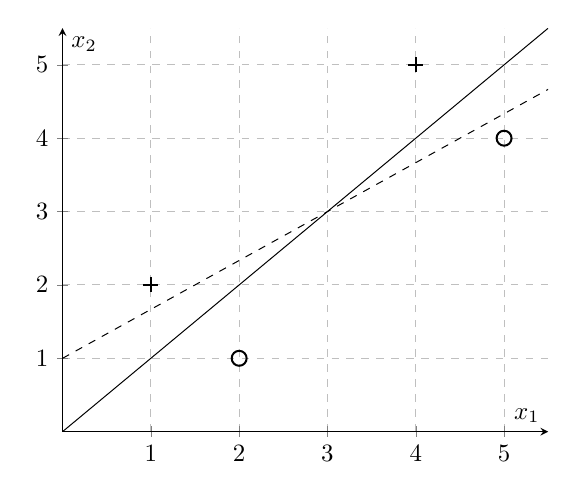
\begin{tikzpicture}[scale=0.9]
\begin{axis}[
    axis lines = center, xlabel = $x_1$, ylabel = $x_2$,
    xtick={0,1,2,3,4,5},ytick={0,1,2,3,4,5},
    ymajorgrids = true,xmajorgrids = true,grid style = dashed,]
%points defined +1
\addplot[only marks, thick, color=black, mark = +, mark size = 3pt]coordinates {(4,5)(1,2)};
%points defined -1
\addplot[only marks, thick, color = black, mark = o, mark size = 3pt]coordinates {(5,4)(2,1)};
%Below the black line is defined
\addplot [dashed,domain = 0:5.5, samples = 10, color = black,]{1/1.5 * x + 1};
%The gray line is defined
\addplot [domain = 0:5.5, samples = 10, color = black,]{x};
\end{axis}
\end{tikzpicture}
\caption{A 2-dimensional example of different possible separating hyperplanes that correctly classify all the toy data points.}
\label{fig:possiblesephyp}
\end{minipage}
\hfill
\begin{minipage}[b]{0.45\textwidth}
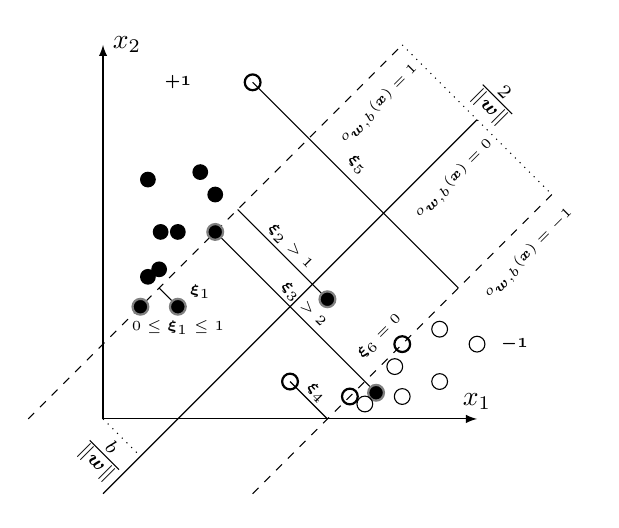
\begin{tikzpicture}[scale = 0.95]
  % Draw axes
  \draw [-latex] (0,0)--(0,5) node  [right]{$x_2$};
  \draw [-latex] (0,0)--(5,0) node  [above]{$x_1$};
  % draw line
  \draw (0,-1) -- (5,4); % y=x-1
  \draw[dashed] (-1,0) -- (4,5); % y=x+1
  \draw[dashed] (2,-1) -- (6,3); % y=x-3
  % \draw labels
  \draw (4.7,3.2) node[rotate=45,font=\tiny] {$o_{\bm w,b}(\bm{x}) = 0$};
  \draw (3.7,4.2) node[rotate=45,font=\tiny] {$o_{\bm w,b}(\bm{x}) = 1$};
  \draw (5.7,2.2) node[rotate=45,font=\tiny] {$o_{\bm w,b}(\bm{x}) = -1$};
  % draw distance
  \draw[dotted] (4,5) -- (6,3);
  \draw (5.25,4.25) node[rotate=-45] {$\frac{2}{\Vert \bm{w} \Vert}$};
  \draw[dotted] (0,0) -- (0.5,-0.5);
  \draw (0,-0.5) node[rotate=-45] {$\frac{b}{\Vert \bm{w} \Vert}$};
  \draw (1,1.5) -- (0.75,1.75);
  \draw (1.3,1.7) node [font=\tiny] {$\bm{\xi}_1$};
  \draw (1,1.225) node [font=\tiny] {$0 \leq \bm{\xi}_1 \leq 1$};
  \draw (3,1.6) -- (1.8,2.8);
  \draw (2.5,2.3) node [rotate=-45, font=\tiny] {$\bm{\xi}_2 > 1$};
  \draw (3.65,0.35) -- (1.5,2.5);
  \draw (2.675,1.525) node [rotate=-45, font=\tiny] {$\bm{\xi}_3 > 2$};
  \draw (2.5,0.5) -- (3,0);
  \draw (2.85,0.35) node [rotate=-45, font=\tiny] {$\bm{\xi}_4$};
  \draw (2,4.5) -- (4.75,1.75);
  \draw (3.4,3.4) node [rotate=-45, font=\tiny] {$\bm{\xi}_5$};
  \draw (5.5,1) node [font=\tiny] {$\bm{-1}$};
  \draw (1,4.5) node [font=\tiny] {$\bm{+1}$};
  \draw (3.7,1.1) node [rotate=45,font=\tiny] {$\bm{\xi}_6 = 0$};
  % draw negative dots
  \draw[thick, draw=gray, fill=black] 	(0.5,1.5) 	circle (3pt);
  \draw[thick, draw=gray, fill=black]   (1.5,2.5)   circle (3pt);
  \draw[thick, draw=gray, fill=black] 	(1,1.5)     circle (3pt);
  \draw[thick, draw=gray, fill=black] 	(3,1.6)     circle (3pt);
  \draw[thick, draw=gray, fill=black] 	(3.65,0.35)     circle (3pt);
  \fill[black] 	(1,2.5)     circle (3pt);
  \fill[black] 	(0.75,2)    circle (3pt);
  \fill[black] 	(0.6,1.9)   circle (3pt);
  \fill[black] 	(0.77, 2.5) circle (3pt);
  \fill[black] 	(1.5,3)     circle (3pt);
  \fill[black] 	(1.3,3.3)   circle (3pt);
  \fill[black] 	(0.6,3.2)   circle (3pt);
  % draw positive dots
  \draw[black,thick] (4,1)     circle (3pt); 
  \draw[black,thick] (3.3,.3)  circle (3pt); 
  \draw[black,thick] (2,4.5)  circle (3pt);
  \draw[black,thick] (2.5,0.5)  circle (3pt);
  \draw[black]     (4.5,1.2) circle (3pt); 
  \draw[black]     (4.5,.5)  circle (3pt); 
  \draw[black]     (3.9,.7)  circle (3pt); 
  \draw[black]     (5,1)     circle (3pt); 
  \draw[black]     (3.5,.2)  circle (3pt); 
  \draw[black]     (4,.3)    circle (3pt); 
\end{tikzpicture}
\caption{An illustration of the soft margin SVM solution on an example $2$-dimensional non-linearly separable dataset.}
\label{fig:nonlinsepdata}
\end{minipage}
\end{figure}

The goal of the soft margin SVM classifier is to find a classification function
\begin{equation}
\centering
f(\bm x) = \textsc{sign } o_{\bm w,b}(\bm x),
\label{eq:classificationfunction}
\end{equation}
where $o_{\bm w,b}(\bm x) = \bm{w}\cdot\bm{x}_i+b$ is a linear decision (output) function representing an affine mapping function $o: \reals^d \rightarrow \reals$ and is parameterized by $\bm w \in \reals^d$, the weight vector, and $b \in \reals$, the bias term. In addition, $\bm w$ and $b$ must satisfy the following,
\begin{equation}
y_i\left( \bm{w} \cdot \bm{x}_i + b\right) \geq 1 - \xi_i, \forall i \in \{1,\ldots,n\},
\label{eqn:softsvmconstraint}
\end{equation}
where $\bm \xi \in \reals^n$ are the non-negative slack variables that allow for some classification error to account for overlapping datasets. The minimal distance between points belonging to opposite classes and the hyperplane is defined as the \textit{margin} and has a width equal to $\frac{2}{||\bm{w}||}$, which is why the $\norm{\bm w}$ must be minimal in order to maximize the margin. 

In the example shown in Figure~\ref{fig:possiblesephyp}, if the training data points are slightly moved, the solid line (with the larger margin) will still correctly classify all the instances, whereas the dotted line (with a much smaller margin, comparatively) will not. This illustrates that the location of the hyperplane has a direct impact on the classifiers generalization capabilities. The hyperplane with the largest margin is called the \textit{optimal separating hyperplane}. Figure~\ref{fig:nonlinsepdata} shows the optimal separating hyperplane for overlapping training data points, where the filled data points are from the $+1$ class and the non-filled data points are from the $-1$ class. The training data points on the separating hyperplane (the circled data points), whose decision function value equals $+1$ or $-1$, are called the \textit{support vectors}. 

The soft margin SVM is a result of the following optimization problem:
\begin{equation}
\label{eq:softsvm}
\begin{aligned}
\min\limits_{(\bm{w},b)} &{\,\,\,\,} \frac{1}{2}||\bm{w}||^2 + C\sum_{i=1}^n \xi_i \\
\text{s.t.} & {\,\,\,\,} y_i\left( \bm{w} \cdot \bm{x}_i + b\right) \geq 1 - \xi_i, {\,\,} \forall i \in \{1,\ldots,n\} \\
 & {\,\,\,\,} \xi_i \geq 0, {\,\,} \forall i \in \{1,\ldots,n\},
\end{aligned}
\end{equation}
where the penalty parameter $C \in \reals$ controls the trade-off between margin maximization and classification error minimization, penalizing large norms and errors. Note that Equation~\ref{eq:softsvm} is a classic quadratic optimization problem with linear constraints, and consequently, it has a unique solution. In geometric terms of SVM, this means that there is a one unique separation boundary in the input space with a maximal margin.

Equation~\ref{eq:softsvm} can be rewritten as a regularized loss minimization problem by representing the constraints as the Hinge loss, given by:
\begin{equation}\label{eqn:hingeloss}
\centering
L(y_i,\, o_{(w,b)}(\bm{x}_i)) = \max \set{0, 1 - y_i o_{(w,b)}(\bm{x}_i)},
\end{equation}
which penalizes errors satisfying the following: $ y_i o_{(w,b)}(\bm{x}_i) < 1$ and is a crucial element that facilitates the SVM model's sparseness. The soft margin SVM represented as a regularized loss minimization problem becomes:
\begin{equation}
\label{eqn:reghingeloss}
\min\limits_{\bm (\bm{w},b) \in \mathcal{H}_o \times \reals} R {\,\,} = {\,\,} \frac{1}{2}||\bm{w}||^2 + C\sum_{i=1}^n L(y_i,\, o_{(w,b)}(\bm{x}_i)),
\end{equation}
where $\mathcal{H}_o$ is a general Hilbert space. To handle cases when the data are non-linearly separable, while enhancing the classifier's generalization capabilities, a kernel function can be used~\cite{Aizerman67theoretical}, as shown in Equation~\ref{eq:kerneltrick}:
\begin{equation}
\spa{K}\left(\bm{x}_i,\bm{x}_j\right) = \langle \phi\left(\bm{x}_i\right),\,\phi\left(\bm{x}_j\right)\rangle,
\label{eq:kerneltrick}
\end{equation}
where $\phi(\cdot)$ represents a mapping function from the original feature space to a higher dimensional space. The advantage of utilizing kernels is being able to calculate the inner product in the input space rather than in the very high feature dimensional space (including the infinite dimensional ones). The SVM model output, $o$ shown in Equation~\ref{eq:output}, for a given input vector $\bm{x}$ is defined by the kernel as given below:
\begin{equation}
o(\bm x) = \sum_{i = 1}^n \alpha_i \mathcal{K}(\bm x, \bm{x}_i) + b,
\label{eq:output}
\end{equation}
where $\alpha_i \in \reals$ are the coefficients, or weights, of the expansion in feature space, and $b \in \reals$ is the so-called bias term. Note that if a positive definite kernel is used, there is no need for a bias term $b$, but $b$ can nevertheless be used. The two terms, $\bm \alpha$ and $b$, parametrize the SVM model. A model is called \textit{dense} if the absolute value of all its weights are greater than $0$, while a \textit{sparse} model would be one that contains some $\alpha_i = 0$. The level of sparseness may vary, but the sparser the model, the more scalable the applications.

\section{Support Vector Regression}
The support vector machine was applied to the regression case~\cite{Drucker1997,vapnik1997support}, maintaining all the maximal margin algorithmic features. Unlike pattern recognition problems where the desired outputs $y_i$ are discrete, for the regression case they are continuous, real-valued, function outputs. Given training dataset $\mathcal{S} = \set{(\bm x_1,y_1), \ldots, (\bm x_n,y_n) \in \reals^d \times \reals}$, where $y_i \in \reals$ is the continuous output of input $\bm x_i \in \reals^d$, the goal is to learn a function $f(\bm x)$ with at most $\epsilon$ deviation from the true targets $y_i$ for all the training data, while being as flat as possible. This was introduced by Vapnik's linear loss function with $\epsilon$-insensitivity zone, illustrated in Figure~\ref{fig:epsloss} and given by:
\begin{equation}
\label{eq:epsloss}
\centering
|y_i - o_{(w,b)}(\bm{x_i})|_\epsilon = \begin{cases} 
															0 & if |y_i - o_{(w,b)}(\bm{x_i})| \leq \epsilon \\
															|y_i - o_{(w,b)}(\bm{x_i})| - \epsilon & \text{otherwise}.
														\end{cases}
\end{equation}
The loss is equal to 0 if the difference between the predicted and true output values is less than $\epsilon$. Vapnik's $\epsilon$-insensitivity function, shown in Equation~\ref{eq:epsloss}, defines an $\epsilon$-tube, illustrated in Figure~\ref{fig:regressionsvm}. If the predicted value is within the tube, no loss is incurred~\cite{Kecman2001}. Estimating a linear regression hyperplane is achieved by minimizing:
\begin{equation}
\label{eq:regsvmemp}
\min\limits_{(\bm{w},b) \in \mathcal{H}_o \times \reals} R {\,\,} = {\,\,} \frac{1}{2}||\bm{w}||^2 + C\sum_{i=1}^n (|y_i - o_{(w,b)}(\bm{x_i})|_\epsilon).
\end{equation}
Equation~\ref{eq:regsvmemp} is equivalent to the following, where non-negative slack variables are introduced:
\begin{equation}
\label{eq:softsvropt}
\begin{aligned}
\min\limits_{(\bm{w},b,\bm \xi,\bm \xi^*)} & {\,\,\,\,} \frac{1}{2}||\bm{w}||^2 + C\sum_{i=1}^n{\left(\xi_i + \xi^*_i \right)} \\
\text{s.t.} & {\,\,\,\,} y_i - \bm{w} \cdot \bm{x}_i  - b \leq \xi_i + \epsilon, {\,\,} \forall i = \set{1,\ldots,n}\\
				 & {\,\,\,\,} \bm{w} \cdot \bm{x}_i + b - y_i \leq \xi_i^* + \epsilon, {\,\,} \forall i = \set{1,\ldots,n} \\
				 & {\,\,\,\,} \xi_i, \xi^*_i \geq 0, {\,\,} \forall i = \set{1,\ldots,n}.
\end{aligned}
\end{equation}
Note that the constant $C$ influences the trade-off between approximation error and the model generalizability, similar to the classification setting. 
\begin{figure}[t!]
\centering
\begin{minipage}[b]{0.45\textwidth}
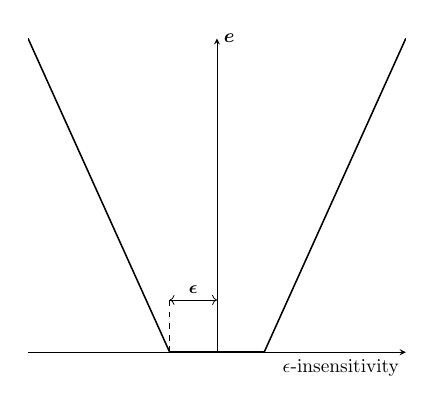
\begin{tikzpicture}[scale=0.7]
\begin{axis}[
	ticks=none,
    axis lines = center, 
    xlabel = $\epsilon\text{-insensitivity}$, 
    xlabel style={below left},
    ylabel = $\bm e$,
    ylabel style={ right}]
% negative epsilon intensity
\addplot [
	thick,
    domain=-4:-1, 
    samples=2, 
    color=black,
]
{- x - 1};
% 0 epsilon intensity
\addplot [
	very thick,
    color=black,
]
coordinates {(-1, 0) (1, 0)};
% positive epsilon intensity
\addplot [
	thick,
    domain=1:4, 
    samples=2, 
    color=black,
]
{ x - 1};
% vertical line indicating where epsilon begines
\addplot[
	color=black,
	style=dashed,
]
coordinates {(-1, 0) (-1, 0.5)};
% epsilon node
\draw[<->] (-1, 0.5) -- (0, 0.5);
\draw (-0.5,0.6) node[font=\small] {$\bm \epsilon$};
\end{axis}
\end{tikzpicture}
\caption{Vapnik's $\epsilon$-insensitivity loss function.}
\label{fig:epsloss}
\end{minipage}
\hfill
\begin{minipage}[b]{0.45\textwidth}
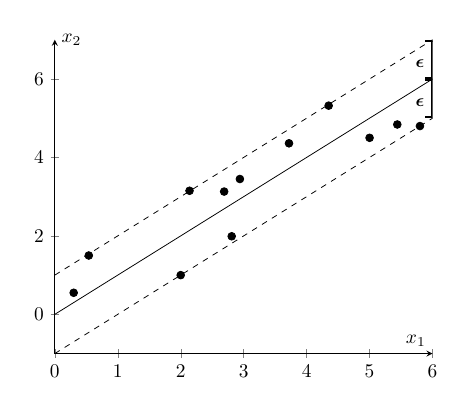
\begin{tikzpicture}[scale = 0.7]
\begin{axis}[
	%ticks = none, 
	axis lines = left, 
	xlabel = $x_1$, 
	xlabel style={at={(1,0)}, above left},
	ylabel = $x_2$,
	ylabel style={at={(0,1)}, right,rotate=-90}
    ]
% main function x
\addplot [
    domain=0:6, 
    samples=2, 
    color=black,
]
{x};
% margin function x + eps
\addplot [
	dashed,
    domain=0:6, 
    samples=2, 
    color=black,
]
{ x+1};
% margin function x - eps
\addplot [
	dashed,
    domain=0:6, 
    samples=2, 
    color=black,
]
{ x - 1};
% epsilon margin
\draw[|-|,very thick] (6,7) -- (6,6);
\draw[|-|,very thick] (6,6) -- (6,5);
\draw (5.8,6.4) node[font=\small] {$\bm \epsilon$};
\draw (5.8,5.4) node[font=\small] {$\bm \epsilon$};
\addplot[color=black,only marks, mark size=2] coordinates {(0.54,1.5) (2,1) (2.14,3.15) (2.94,3.45) (5.8,4.8) (0.30,0.55) (2.69,3.13) (2.81,1.99) (3.72,4.36) (4.35,5.32) (5.44,4.84) (5,4.5) };
\end{axis}
\end{tikzpicture}
\caption{Support vector regression example solution.}
\label{fig:regressionsvm}
\end{minipage}
\end{figure}
The optimization function given in~\ref{eq:softsvropt} can be solved more easily in its dual formulation and is key to extending the SVR to learn from non-linear functions~\cite{Schoelkopf2002}. It is as follows:
\begin{equation}
\label{eq:dualSVR}
\centering
\begin{aligned}
\max\limits_{(\bm \alpha, \bm \alpha^*)} & {\,\,\,\,} -\frac{1}{2} \sum_{i,j = 1}^n (\alpha_i - \alpha^*_i)(\alpha_j - \alpha^*_j)\mathcal{K}(\bm x_i, \bm x_j)  - \epsilon \sum_{i=1}^n (\alpha_i + \alpha^*_i) + \sum_{i=1}^n y_i (\alpha_i - \alpha^*_i) \\
 \text{s.t.} & {\,\,\,\,} \sum_{i=1}^n (\alpha_i - \alpha^*_i) = 0,\, \alpha_i, \alpha^*_i \in [0, C],\, \forall i = \set{1,\,\ldots,n},
 \end{aligned}
\end{equation}
where $\bm \alpha$ and $\bm \alpha^*$ correspond to the SVR dual variables.  

\section{Support Vector Machine Solvers}
Although support vector machines represent a major development in machine learning algorithms, in the case of large-scale problems (hundreds of thousands to several millions of samples), the design of SVM training algorithms still has room for improvement. 

%So far, there have been various approaches for tackling large-scale SVM classification problems.

% Add a sentance for how it first started.. with this.
\textit{Interior Point} (IP) methods pose the SVM learning problem as a quadratic optimization problem subject to linear constraints, which are then replaced with a barrier function~\cite{Boyd2004}. The resulting unconstrained problem can then be optimized using Newton or Quasi-Newton methods. However, IP methods typically require a run time of $[O(n^3)]$. Moreover, the memory requirements of IP methods are $[O(n^2)]$, rendering the use of IP methods impractical when the training set consists of a large number of samples. 

The first attempts of overcoming the quadratic memory requirement of IP methods and speeding up their training time were aimed at \textit{decomposing} the underlying SVMs quadratic programming problem. First, Boser et al.~\cite{boser1992training} implemented Vapnik's \textit{chunking} method. \textit{Sequential Minimal Optimization} (SMO) by Platt~\cite{Platt1998}, its improvement by Keerthie et al.~\cite{keerthi2001improvements}, and SVM-Light~\cite{Joachims1999} are alternative approaches to decomposing the QP problem. SMO, implemented in the popular, widely used software package LIBSVM~\cite{CC01a}, is an iterative procedure that divides the SVM dual problem into a series of sub-problems, which are solved analytically by finding the optimal $\bm \alpha$ values that satisfy the Karush-Kuhn-Tucker conditions~\cite{Boyd2004}. Although SMO is guaranteed to converge, heuristics are used to choose $\bm \alpha$ values in order to accelerate the convergence rate. This is a critical step because the convergence speed of the SMO algorithm is highly dependent on the dataset size and SVM hyperparameters~\cite{Schoelkopf2002}.

Most existing approaches, including the methods described above, focus on solving the dual of Equation~\ref{eq:softsvm}, for two main reasons: firstly, the dual formulation provides a convenient way of dealing with the constraints. Secondly, the dual formulation can be written in terms of dot products, allowing the use of kernel functions~\cite{bottou2007large}. However, these two conveniences are not restrictions for solving \textit{primal} SVM problem. For example, Chappelle~\cite{Chapelle2007} showed that even though optimizing the primal and dual are equivalent in terms of solutions and time, optimizing the primal when dealing with approximate solutions is far more superior. The primal problem can be cast as an unconstrained problem by using linear or non-linear kernels and the Representer theorem~\cite{scholkopf2001generalized}; mainly, reparametrizing the weight vector. Chapelle~\cite{Chapelle2007} investigated solving the primal objective with smooth loss functions, rather than using the hinge loss function, and suggested using methods such as conjugate gradient descent and Newton's method.

Some advancements in handling large scale problems are based on a \textit{geometric} interpretation of SVM problem. Some of these geometric SVMs include approaches that use convex hulls~\cite{bennett2000duality} and minimum enclosing balls such as \textit{Core Vector Machines} (CVM)~\cite{tsang2005core}. Tsang et al.~\cite{tsang2007simpler} later improved the scalability of CVMs by introducing \textit{Ball Vector Machines} (BVM) which do not require a QP solver. Other geometric approaches include the novel algorithms introduced by Strack~\cite{strack2013geometric}, known as the \textit{Sphere Support Vector Machine} (SphereSVM) and \textit{Minimal Norm Support Vector Machine} (MNSVM), which utilize the connection between minimal enclosing balls and convex hull problems, while demonstrating a high capability for learning from large datasets. 

The \textit{Non-Negative Iterative Single Data Algorithm} (NNISDA)~\cite{zigic2016} is an efficient approach for solving the SVM problem, shown to be faster than SMO and equal in terms of accuracy~\cite{Kecman2014}. NNISDA is an iterative algorithm that finds a solution to the L2-SVM using \textit{coordinate descent}, inspired by \textit{Iterative Single Data Algorithm} (ISDA)~\cite{Huang2006}, which was originally introduced in~\cite{Kecman2005}.

Recently, several authors have proposed the use of a standard \textit{stochastic} (or \textit{online}) \textit{gradient descent} (SGD) approach for SVMs to optimize large-scale learning problems~\cite{herbrich2016learning,kivinen2002large,Schoelkopf2002,Shalev2014,shalev2011pegasos}. Kivinen et al.\cite{kivinen2004online} and Bousquet and Bottou~\cite{bousquet2008tradeoffs} showed that stochastic algorithms can be both the fastest, and have the best generalization performances. It has also been shown that the SGD runtime for solving the SVM unconstrained primal problem is inversely proportional to the size of the training set~\cite{panagiotakopoulos2013stochastic,shalev2008svm}. Shalev-Shwartz and Ben-David~\cite{Shalev2014} have demonstrated that the basic SGD algorithm is very effective when data are sparse, taking less than linear $[O(d)]$ time and space per iteration to optimize a system with $d$ parameters. It can greatly surpass the performance of more sophisticated batch methods on large data sets. The previously mentioned approaches are extended variants of the classic \textit{kernel perceptron} algorithm~\cite{collobert2004links}. 

Notable representatives of this method of learning include the \textit{Na{\"i}ve Online R Minimization Algorithm} (NORMA) by Kivinen et al.~\cite{kivinen2004online} and the \textit{Primal Estimated Sub-Gradient SOlver for Support vector machines} (PEGASOS) by Shalev-Shwartz et al.~\cite{shalev2011pegasos}. NORMA is an online kernel based algorithm designed to utilize SGD for solving the SVM problem, exploiting the kernel trick in an online setting. It can be regarded as a generalization of the kernel perceptron algorithm with regularization~\cite{kivinen2004online}. PEGASOS solves the primal SVM problem using stochastic sub-gradient descent, implementing both linear and non-linear kernels, and showed that the algorithm does not directly depend on the size of the data, making it suitable for large-scale learning problems. 

A more recent approach, named \textit{OnLine Learning Algorithm} (OLLA)~\cite{kecman2016fast} is a unification, simplification, and expansion of the somewhat similar approaches presented in
~\cite{herbrich2016learning,kivinen2002large,Schoelkopf2002,Shalev2014,shalev2011pegasos} and~\cite{kecman2016ieee,Melki2016,melki2016fast}. This algorithm is unique because it is not only designed to optimize the SVM cost function, but also the cost functions of several other popular nonlinear (kernel) classifiers using SGD in the primal domain. Collobert and Bengio~\cite{collobert2004links} provided justification for not using regularization, and thus OLLA was designed to handle cost functions with and without the regularization term. Comparisons of performances of OLLA with the popular SMO algorithm highlighted the merits of OLLA in terms of speed, as well as accuracy, when the number of samples was increased, making it suitable for large-scale learning. Comparisons using various different classifiers against SMO were also shown in~\cite{kecman2016fast}, but for the scope of this thesis the L1-SVM was mentioned.

Although the SGD approaches mentioned above have many merits when it comes to solving large-scale machine learning problems, stochastic procedures also have their disadvantages. One of them stems from the lack of meaningful stopping criteria. The only specified stopping criteria is a user defined input for the number of iterations, which gives rise to the question of what it should be set to. Another unknown parameter that requires tuning is the gradient step size, which in some cases, directly affects the algorithm convergence rate. Moreover, a third disadvantage of kernelized online algorithms is that the training time for each update increases superlinearly with the number of samples~\cite{bottou2004large}.

\section{Why Support Vector Machines: Form \& Norm}
The support vector machine problem shares similarities to classical statistical inference such as Neural Networks (NNs), however, there are several very important differences between their approaches and assumptions. 

One of the major differences is that these traditional classification and regression statistical techniques are based on the strict assumption that the data distribution is known and is that of a Gaussian distribution. Another assumption is that this data can be modeled by a set of linear parameter functions. Following this, the induction paradigm for parameter estimation is the maximum likelihood estimation method, which can be reduced to the minimization of the sum-of-errors-squared cost function~\cite{Kecman2001}. 

The previously stated assumptions, on which the classic statistical paradigm relied, turned out to be inappropriate for many contemporary problems for a couple of reasons~\cite{vapnik1997support} . Real-world problems are, more often than not, high-dimensional. If the underlying mapping is not smooth, the linear paradigm needs an exponentially increasing number of terms, thus increasing the dimensionality of the input space, also known as `\textit{the curse of dimensionality}'. Another issue is that the data generation process might be very different from the normal distribution. Due to these grave concerns, the maximum likelihood estimator or sum-of-errors-squared cost function, should be replaced by a new induction paradigm to be able to model non-Gaussian distributions, or rather, to have a distribution-free method of classification or regression for high-dimensional, sparse data~\cite{Kecman2001}. This was the foundational reason for developing support vector machines.

The main differences between SVMs and classical statistical techniques, such as NNs, can be identified by analyzing their \textit{form} and \textit{norm}. With respect to both types of models' \textit{form}, the greatest majority of machine learning models are the same, i.e. they are represented as the sum of weighted basis functions. The difference in the two approaches stems from their \textit{norm} (cost functions) and how these models learn their function parameters (e.g. how many functions should be used, what their parameters are, what the value of their weights should be). 

For example, NNs minimize the sum-of-errors-squared in output space, i.e. the L2 norm, and SVMs maximize the margin in input space by minimizing the L2 norm of the weight vector. For SVMs, the model parameters are not predefined and their number depends on the training data used. Rather than choosing the appropriate structure of the model, keeping the estimation error fixed, and minimizing the training error, as done by classical techniques, SVMs keep the training error fixed or set to some appropriate level and minimize the estimation error. This is the paradigm of structural risk minimization (SRM) introduced by Vapnik and Chervonenkis and their colleagues, which led to the new learning algorithm. This approach has been proven, both experimentally and theoretically, to be superior (or comparable) to NNs and other statistical methods for contemporary real-world problems, which are often very sparse datasets (i.e. small number of samples in high dimensional spaces).

\chapter{Multi-Target SVR using Maximum Correlation Chains}\label{chap:mtr}
This chapter presents three multi-target support vector regression (SVR) models. The first involves building independent, single-target SVR models for each output variable. The second builds an ensemble of random chains using the first method as a base model, named SVR with Random Chains (SVRRC), inspired by the classification MT method, Ensemble of Random Chains Corrected (ERCC)~\cite{Spyromitros2014}. The third calculates the targets' correlations and forms a maximum correlation chain, which is used to build a single chained model named SVR with Correlation Chaining (SVRCC). The experimental study compares the performance of the three approaches with six other prominent MT regressors. The experimental results are then analyzed using non-parametric statistical tests. The results show that the maximum correlation SVR approach improves the performance of using ensembles of random chains. 

This chapter is organized as follows: Section~\ref{sec:MTRbackground} describes the notation used throughout this chapter and reviews related works on multi-target regression. Section~\ref{sec:MTRproposal} presents the three multi-target support vector regression approaches. Section~\ref{sec:MTRexperiments} presents the experimental study. Section~\ref{sec:MTRresults} discusses the results and the statistical analysis. Finally, Section~\ref{sec:MTRconclusions} shows the main conclusions of this work.

\section{Multi-Target Regression Background}\label{sec:MTRbackground}
This section first defines the notation that will be used throughout this chapter, and then formally describes the multi-target regression problem along with relevant popular algorithms used within this paradigm.

\subsection{Notation}\label{subsec:mtrnotation}
\begin{table*}[t!]
\small \centering
\caption{Multiple-Target Learning Notation}
\resizebox{\textwidth}{!}{\begin{tabular}{ll}
\noalign{\smallskip}\hline\noalign{\smallskip}
Definition & Notation\\ 
\noalign{\smallskip}\hline\noalign{\smallskip}
Number of Samples & $\mathcal{N}$ \\
Number of Input Attributes & $d$ \\
Input Space & $\bm{X} \in \mathbb{R}^{\mathcal{N} \times d},\,1\leq i \leq d$ \\
Input Instance & $\bm{x}^{(l)} = (x_1^{(l)}, \ldots, x_d^{(l)}) \in \bm{X},\, 1 \leq l \leq\mathcal{N}$ \\
Number of Dataset Targets/Outputs & $m$ \\
Target Space & $\bm{Y} = \{\bm Y_1, \ldots, \bm Y_j, \ldots, \bm Y_m\} \in \mathbb{R}^{\mathcal{N} \times m},\, 1 \leq j \leq m$ \\
Predicted Target Space & $\bm{\hat{Y}} = \{\bm{\hat{Y_1}}, \ldots, \bm{\hat{Y_j}}, \ldots, \bm{\hat{Y}_m}\} \in \mathbb{R}^{\mathcal{N} \times m},\, 1 \leq j \leq m$ \\
\vspace{1.5pt}
Target Instance & $\bm y^{(l)} = (y_1^{(l)}, \ldots, y_m^{(l)}) \in \bm{Y},\,1 \leq l \leq\mathcal{N}$ \\
\noalign{\smallskip}\hline\noalign{\smallskip}
\noalign{\vskip 0.04in}
Full Multi-Target (MT) Training Dataset & $\mathcal{D} = \{(x_1^{(1)},y_1^{(1)}), \ldots, (x_d^{(\mathcal N)},y_m^{(\mathcal N)})\}$ \\
Single-Target (ST) Dataset with $j^{th}$ Target & $\mathcal{D}_j = \{(x_1^{(1)},y_j^{(1)}), \ldots, (x_d^{(\mathcal N)},y_j^{(\mathcal N)})\} \in \mathcal{D},\, 1 \leq j \leq m$\\
Number of Cross-Validation (CV) Sets & $k$ \\
ST Test Dataset with $j^{th}$ Target, $i^{th}$ CV Fold & $\mathcal{D}_j^{(i)} = \{(x_1^{(i)},y_j^{(i)}), \ldots, (x_d^{(i)},y_j^{(i)}) \in \mathcal{D}_j,\, i \in \{1,\ldots,\mathcal{N}\}$ \\
ST Training Dataset with $j^{th}$ Target, Excluding the $i^{th}$ CV Fold & $\mathcal{D}_j^{(k-i)} = \mathcal{D}_j \setminus \mathcal{D}_j^{(i)}$ \\
ST Regression Model & $h : \bm{X} \times \bm{Y}$ \\
MT Regression Model & $h_j : \bm{X} \times \bm{Y}_j,\, 1 \leq j \leq m$ \\
Unknown Sample & $\bm{x}^{(\mathcal N^\prime)} = \{\bm {x}^{(\mathcal N+1)}, \ldots, \bm {x}^{\mathcal (N^\prime)}\}$ \\
Predicted Values for Unknown Sample & $\bm{y}^{(\mathcal N^\prime)} = \{\bm{y}^{(\mathcal N+1)}, \ldots, \bm {y}^{(\mathcal N^\prime)}\}$\\
\noalign{\smallskip}\hline\noalign{\smallskip}
\end{tabular}}
\label{tab:mtrNotation}
\end{table*}
Let $\mathcal{D}$ be a training dataset of $n$ instances. Let $\bm{X} \in \mathcal{D}$ be a matrix consisting of $d$ input variables and $n$ samples, such that $\bm{X} \in \mathbb{R}^{n \times d}$. Let $\bm{Y} \in \mathcal{D}$ be a matrix consisting of $m$ continuous target variables and $n$ samples,  where $\bm{Y} \in \mathbb{R}^{n \times m}$. Table~\ref{tab:mtrNotation} summarizes the notation used throughout this chapter.

\subsection{Multi-Target Regression Methods}
As mentioned previously, there are two main approaches to solving multiple-output problems: \textit{problem transformation} and \textit{algorithm adaptation.} This section will present the theory behind both approaches, their advantages and disadvantages, as well as current popular solvers.

Problem transformation methods are mainly based on training $m$ independent, single-target models for each target outout on datasets $\mathcal{D}_j = \set{\bm X, \bm Y_j},\, \forall j \in \{1, \ldots, m\}$ and concetenating all $m$ predictions. The \textit{single-target} method~\cite{Spyromitros2014}, also known as binary relevance in literature~\cite{Zhang20141819}, simply does exactly that, and is considered as a baseline for measuring the performance of other problem transformation approaches. Since this approach divides the multi-target problem into $m$ single-target ones, any off-the-shelf traditional regression algorithm can be used. Examples include ridge regression~\cite{hoerl1970ridge}, regression trees~\cite{Breiman1996}, and support vector regression~\cite{Drucker1997}.

The main drawback with single-target approaches in the multi-target setting, is that the relationships between the targets are lost once independent models are built for each target. This in turn may affect the overall quality of the $m$ predictions~\cite{Borchani2015}. Another drawback of this type of approach is computational complexity: prediction for an unseen sample would be obtained by running each of the $m$ single-target models and concatenating their results. 

Recently, Spyromitros-Xioufis et al.~\cite{Spyromitros2014} proposed extending well-known multi-label classification methods to deal with the multi-target regression problem, while modeling the targets' dependencies. Inspired by their successful classification counterparts, Spyromitros-Xioufis et al.~\cite{Spyromitros2014} introduced two novel approaches for multi-target regression: multi-target regressor stacking (MTS) and regressor chains (RC). These methods involve two stages of learning, the first being building ST models; and the second uses the knowledge gained by the first step to predict the target variables while using possible relationships the targets might have with one another. 

Multi-target regressor stacking was inspired by its multi-label classification counterpart~\cite{godbole2004discriminative} and involves two stages of training. The first stage consists of training $m$ independent single-target models, like in ST. In the second step, a second set of $m$ meta models are learned for each target variable, $\bm{Y}_j,\, 1 \leq j \leq m$. These meta models are learned on a transformed dataset, where the input attributes space is expanded by adding the approximated target variables obtained in the first stage, excluding the $j^{th}$ target being predicted.

The regressor chains method, also inspired by an equivalent multi-label classification method~\cite{read2011classifier}, is another problem transformation method, based on the idea of chaining a sequence of single-target models. In the training of RC, a random chain (sequence) of the set of target variables is selected and for each target in the chain, models are built sequentially by using the output of the previous model as input for the next~\cite{Xioufis2016}, following the order of the chain. 

If the default, ordered chain is $C = \{\bm Y_1, \bm Y_2, \ldots, \bm Y_m\}$, the first model $h_1 : \bm X \rightarrow \mathbb{R}$ is trained for $\bm Y_1$, as in ST. For the subsequent models $h_{j,j>1}$, the dataset is transformed by sequentially appending the true values of each of the previous targets in the chain to the input vectors. For a new input vector, the target values are unknown. Once the models are trained, the unseen input vector will be appended with the approximated target values, making the models dependent on the approximated values obtained at each step. One of the issues associated with this method is that, if a single random chain is used, the possible relationships between the targets at the head of the chain and the end of the chain are not exploited due to the algorithm's sequential nature. 

In the methods described above, the estimated target variables (meta-variables) are used as input in the second stage of training. In both methods, the models are trained using these meta-variables that become noisy at prediction time, and thus the relationship between the meta-variables and target variable is muddied. Dividing the training set into sets, one for each stage, would not help this situation because both methods would be trained on training sets of decreasing size. Due to these issues, \textit{Spyromitros et. al.} proposed modifications, in \cite{Spyromitros2014}, to both methods that resembles $k$-fold cross-validation (CV) to be able to obtain unbiased estimates of the meta-variables. These methods are called Regressor Chains Corrected (RCC) and Multi-Target Stacking Corrected (MTSC). 

However, these corrections did not solve all the methods' problems. One problem with the RC and RCC methods was that they are sensitive to the chain ordering. To remedy this issue, Spyromitros-Xioufis et al.~\cite{Spyromitros2014} proposed the Ensemble of Regressor Chains (ERC) and Ensemble of Regressor Chains Corrected (ERCC). Instead of a single chain, $k \leq 10$ chains are created at random, and the final prediction values are obtained by taking the mean values of the $k$ predicted values for each target. The ERC, ERCC and MTSC procedures involve repeating the RCC and MTS procedures $k$ times, respectively, with $k$ randomly ordered chains for ERCC, and $k$ different modified training sets for MTSC. The corrected methods exhibited better performance than their original variants, as well as ST models. The ERCC algorithm had the best overall performance, as well as being statistically significantly more accurate of all the methods tested\cite{Spyromitros2014}.

Many authors have proposed using support vector machines for multi-target learning~\cite{Borchani2015,Xiong2014,Xu2013}. One example is that of Zhang et al.~\cite{Zhang2012}, who presented a multi-output support vector regression approach based on problem transformation. It builds a multi-output model that considers the correlations between all the targets using the vector virtualization method. Basically, it extends the original feature space and expresses the multi-output problem as an equivalent single-output problem, so that it can then be solved using the single-output least squares support vector regression machines (LS-SVR) algorithm. Moreover, other contemporary problem transformation approaches include Linear Target Combinations for MT Regression~\cite{Tsoumakas2014}.

Algorithm adadaptation algorithms are based on the concept of simultaneously predicting all outputs using a single model which captures all dependencies and internal relationships between them. Using this type of approach provides several advantages over problem transformation methods~\cite{breiman1997predicting,kocev2009using,simila2007input}:
\begin{itemize}
\iitem A single multi-taget model is more interpretable than several single-target models.
\iitem When the targets are correlated, algorithm adaptation methods ensure better predictive performance.
\end{itemize}

The first attempts at dealing with predicting multiple real-valued targets at the same time are statistical approaches which aim to capture the possible correlations amongst target variables. One example is reduced-rank regression, proposed by Izenman~\cite{izenman1975reduced}, which places a constraint on the elements of estimated reduced-rank regression coefficient matrices. Brown and Zidek~\cite{brown1980adaptive} then proposed a multivariate version of the Hoerl-Kennard ridge regression rule. More recently Simil{\"a} and Tikka~\cite{simila2007input} considered the regression problem of modeling several output variables using the same set of input variables, chosen by their simultaneous variable selection method, named L$2$-SVS. The importance of an input attribute is measured by the L$2$-norm of their corresponding regression weights, which are found by minimizing the sum-of-errors-squared.

Maximal margin classifiers have also been transformed to accommodate the multi-output case~\cite{tsochantaridis2005large}. Rather than having a single-output support vector regressior be applied independently to each target, several approaches have been proposed to extend the traditional SVR to the multi-output case. One example is that of Vazquez and Walter~\cite{vazquez2003multi}. They extended the traditional SVR by considering the multi-output version of Kringing called Cokringing~\cite{chiles1999}. The authors show that their multi-target SVR produced better results than building independent SVRs. Another example is Brudnak's~\cite{brudnak2006vector} proposal of a vector-valued SVR (VVSVR). Their method generalizes Vapnik's $\epsilon$-insensitive loss function and regulariztion function from the scalar-valued case to that of vector-value.

In addition to maximal margin classifiers being extended to the multi-output case, the use of multi-output kernels has also been investigated. Evgeniou and Pontil~\cite{evgeniou2004regularized} presented an approach to multi-output learning based on minimizing regularized risk functionals, such as SVMs. They proposed a novel kernel function that uses a parameter $\mu$ that couples the targets. Their experiments also supported the fact that using an algorithm adaptation approach does perform well when targets are correlated. However, when the targets are not correlated, Evengiou and Pontil showed that their proposed method reduces to single-target learning when the parameter $\mu$ is set to be very large, posing no risk to using their multi-target kernel. Choosing the right value for $\mu$ must be found by cross-validation. 

Due to the success of using this multi-output kernel approach, Evgeniou et al.~\cite{Evgeniou2005} extended their earlier results and developed a framework for multi-task learning within the context of regularization in reproducing kernel Hilbert spaces. A drawback of their proposed kernel method is that its computational complexity time is worse than the complexity of solving $m$ independent kernel methods.

Multiple-target regression trees, also known as multi-variate or multi-objective regression trees, are extensions of the traditional regression tree to the multi-output case. One of the first approaches for building multi-target regression trees was that of De'ath~\cite{de2002multivariate}, who proposed an extension of the univariate method CART~\cite{breiman1984classification} to the multi-output case, dubbed multi-variate regression trees (MRTs). The main difference between the traditional CART and its multi-variate extension is the redefinition of the impurity measure of a node to the multi-variate sum-of-squared-errors.

Blockeel et al. proposed multi-objective decision trees (MODTs)~\cite{blockeel1998top,kocev2009using}, which are decision trees capable of predicting multiple target attributes at once and are used for multi-objective prediction. Struyf and D{\v{z}}eroski~\cite{struyf2005constraint} proposed a constraint-based framework for building multi-objective regression trees (MORTs). Later, Kocev et al.~\cite{Kocev2007} investigated whether ensembles of multi-objective decision trees could be used to improve the performance of using multiple single-target trees or a single multi-target tree. The ensemble learning techniques used were bagging~\cite{Breiman1996} and random forests~\cite{breiman2001random}.

The methods described above were all designed to try to analyze and improve the performance of predicting multiple outputs at once, however there are still outstanding issues to be addressed. Considering the models' predictive performances, the benefits of using MTSC and ERCC instead of the baseline ST are are not apparent. In the experimental study performed by Spyromitros-Xioufis et al.~\cite{Spyromitros2014}, the ST method sometimes outperformed their proposed problem transformation approaches. The best explanation for this would be that the targets correlations were not captured due to the \textit{randomized} learning process (chain order). Another issue that these approaches face comes with having a large number of output variables. Due to the ensemble based approach of up to 10 random chains, or solving a large number of single-target problems, the algorithms' computational complexity would suffer. Furthermore, these models do not provide a clear description of the relationship between the input and output variables, as well as the outputs amongst themselves. The contributions of this chapter aim to remedy the mentioned disadvantages.

\section{Three Novel SVMs for Multi-Target Regression}\label{sec:MTRproposal}
Three novel models have been implemented for the purposes of multi-target regression. The base model is the SVR model, where $m$ single-target soft margin non-linear support vector regressors (NL-SVR) are built for each target variable $\bm Y_j$. 
\begin{figure}[b!]
\begin{minipage}{0.9\textwidth}
\small \centering
\[\begin{tikzcd}[column sep = small, row sep = small]
& & \mathcal{D}_1 :  [\bm X][\bm Y_1]  \arrow[rr]  & & h_1 :  \mathcal{D}_1 \rightarrow \bm{\hat{Y_1}}\\
& & \mathcal{D}_2 :  [\bm X][\bm Y_2]  \arrow[rr] & & h_2 :  \mathcal{D}_2 \rightarrow \bm{\hat{Y_2}} \\        
\mathcal{D} :  [\bm X][\bm Y]  \arrow[uurr, bend left=45] \arrow[urr, bend left] \arrow[drr, bend right]  		& & \vdots \\
& & \mathcal{D}_m :  [\bm X][\bm Y_m] \arrow[rr] & & h_m :  \mathcal{D}_m \rightarrow \bm{\hat{Y}_m}
\end{tikzcd}\]
\end{minipage}
\caption{SVR Flow Diagram. Firstly, MT dataset is divided into $m$ ST datasets, $\mathcal{D}_1, \mathcal{D}_2, \ldots, \mathcal{D}_m$. Then $m$ models, $h_1, h_2, \ldots, h_m$, are independently trained for each ST dataset.}\label{diag:SVR}
\begin{algorithm}[H]
\caption{MT Support Vector Regression (SVR)} \label{alg:SVR} 
\small \centering
\begin{algorithmic}[1]
\renewcommand{\algorithmicrequire}{\textbf{Input:}}
\renewcommand{\algorithmicensure}{\textbf{Output:}}
\Require Training dataset $\mathcal{D}$
\Ensure  ST models $h_j, j = 1,\ldots,m$
\For {$j = 1$ to $m$}
\State $\mathcal{D}_j = \{\bm X, \bm Y_j\}$ \Comment{Get ST data}
\State $h_j : \bm X \rightarrow \mathbb{R}$ \Comment{Build ST model for the $j^{th}$ target}
\EndFor \\
\Return $h_j, j=1,\ldots,m$ 
\end{algorithmic} 
\end{algorithm}
\end{figure}

For NL-SVR, the regularized soft margin loss function given in equation~\eqref{eq:softsvropt} is minimized. This contribution involves solving the dual of this formulation given by \eqref{eq:dualSVR}. Using the dual formulation, the multi-target problem is solved by transforming it into $m$ single-target problems, as shown in Algorithm~\ref{alg:SVR} and Figure~\ref{diag:SVR}. This algorithm will output $m$ single-target models, $h_j,\,\forall j = 1,\ldots,m$, for a given dataset $\mathcal{D}$. It first splits the dataset into $m$ separate ones, $\mathcal{D}_j$, each with a single-target variable $\bm Y_j$, and then builds a distinct SVR model for each of the datasets. 

Building $m$ ST models is a good base-line, but as mentioned previously, it does not capture possible correlations between the target attributes during training. If these correlations are not exploited, this could retract from the model's potential performance. Therefore, creating an ensemble model using a series of random chains was proposed, using the base-line SVR method, named SVR Random Chains (SVRRC). 
\begin{algorithm}[t!]
\centering \small
\caption{Build Chained Model}
\label{alg:buildchainedmodel} 
\begin{algorithmic}[1]
\renewcommand{\algorithmicrequire}{\textbf{Input:}}
\renewcommand{\algorithmicensure}{\textbf{Output:}}
\Require Training dataset $\mathcal{D}$, random chain $\bm C$
\Ensure  A chained model $h_j, j = \{1,\ldots,m\}, c \leq 10$
\State $\mathcal{D}_1 = \set{\bm X, \bm Y_{\bm C_1}}$ \Comment{Initialize first dataset}
\For {$j=1$ to $m$} \Comment{For each target in chain $\bm C$}
\State $h_j : \mathcal{D}_j \rightarrow \mathbb{R}$ \Comment{Train model on appended dataset}
\If {$j < m$}
\State $\mathcal{D}_{j+1} = \set{\mathcal{D}_j, \bm Y_{\bm C_j}}$ \Comment{Append new target in chain to dataset}
\EndIf
\EndFor \\
\Return $h_j, j=1,\ldots,m$ 
\end{algorithmic} 
\end{algorithm}

For SVRRC, ensembles of at most $10$ $m$-sized random chains, $\mathcal{C}$, are built from different and distinct permutations of the target variable indices. When chaining target values, there are two main options: using the predicted value as input for the following target, or using the true value of the target variable as input of the subsequent targets. The main problem with the former approach is that errors are propagated throughout the chained model, therefore SVRCC employs chaining of the true values. 

For each random chain, a new model is trained by predicting the first target variable in the chain. Next, the first target's true value, $\bm Y_j$, is appended to the training set. This chaining process is repeated for all the target indices in the chains, $\{\bm C_1, \ldots, \bm C_c\} \in \mathcal{C}, \, c \leq 10 \,$. This process will be repeated for each random chain generated, returning an ensemble of chained SVRs. Algorithm~\ref{alg:buildchainedmodel} describes the process of building a chained model given chain $\bm C \in \mathcal{C}$, and Algorithm~\ref{alg:SVRRC} shows the steps taken by SVRRC. 

Given this ensemble of chained models, the predicted values for a given unseen instance are calculated by taking the mean of the multiple models generated using different random chains. Since the unseen input has no known target value, the predicted value at each step of the chain $\hat{\bm Y}_j$ is appended to the input at each step of the chain. 
\begin{figure}[t]
\centering \small
\begin{minipage}{\textwidth}
\centering \small
\begin{tikzcd}[column sep = small, row sep = small]
& \mathcal{D} :  [\bm X][\bm Y_1 \bm Y_2 \bm Y_3] \arrow[dl] \arrow[d] \arrow[drr] & & \\
\left[1,2,3\right] \arrow[d] & \left[1,3,2\right] \arrow[d] & \hdots & \left[3,2,1\right] \arrow[d] \\
h_1 :  [\bm X] \rightarrow \bm{\hat{Y_1}} \arrow[d] & h_1 :  [\bm X] \rightarrow \bm{\hat{Y_1}} \arrow[d] & \hdots & h_1 :  [\bm X] \rightarrow \bm{\hat{Y_1}} \arrow[d] \\
h_2 :  [\bm X \bm{Y_1} ] \rightarrow \bm{\hat{Y_2}} \arrow[d] & h_2 :  [\bm X \bm{Y_1} ] \rightarrow \bm{\hat{Y_3}} \arrow[d] & \hdots & h_2 :  [\bm X \bm{Y_3} ] \rightarrow \bm{\hat{Y_2}} \arrow[d] \\
h_3 :  [\bm X \bm{Y_1Y_2} ] \rightarrow \bm{\hat{Y_3}} & h_3 :  [\bm X \bm{Y_1Y_3} ] \rightarrow \bm{\hat{Y_2}} & \hdots & h_3 :  [\bm X \bm{Y_3Y_2} ] \rightarrow \bm{\hat{Y_1}}
\end{tikzcd}
\end{minipage}
\caption{SVRRC Flow Diagram on a dataset with 3 targets. SVRRC first builds the $6$ random chains of the target's indices ($3$ examples are shown). It then constructs a chained model by proceeding recursively over the chain, building a model, and appending the current target to the input space to predict the next target in the chain. } \label{fig:svrrc}
\begin{algorithm}[H]
\caption{MT SVR with Random-Chains (SVRRC)}
\small \centering
\label{alg:SVRRC} 
\begin{algorithmic}[1]
\renewcommand{\algorithmicrequire}{\textbf{Input:}}
\renewcommand{\algorithmicensure}{\textbf{Output:}}
\Require Training dataset $\mathcal{D}$, $c$ random chains $\mathcal{C}$
\Ensure  An ensemble of chained models $h_\mathcal{C}$
\For {\textbf{each }$\bm C \in \mathcal{C}$} \Comment{For each random chain}
\State $h_{\bm C} = $ \text{build chained model}$(\mathcal{D},\bm C)$ \Comment{build a chained model for chain $\bm C$}
\EndFor \\
\Return $h_\mathcal{C}$ 
\end{algorithmic} 
\end{algorithm}
\end{figure}

Due to the computational complexity of building $m!$ distinct chains and training $\left(m!\right) \times m$ models, the number of ensembles and chains are limited to a maximum of $10$. However, if the number of target variables is less than $3$, i.e. $m! \leq 10$, all $m!$ random chains are constructed. 

A disadvantage of building an ensemble of 10 random chains stems from the fact that: when the number of output variables increases, the number of possible chains increases factorially. Therefore, there is no guarantee that the 10 random chains generated will truly reflect the relationships among the target variables. Additionally, building an ensemble of regressors is computationally expensive. Finding a heuristic that allows the identification of a single, most appropriate chain, which fully reflects the output variable interrelations would improve the scalability of training the ensemble. 

The third proposal was designed to remedy this issue. It builds a single chain based on the maximization of the correlations among the target variables. By calculating the correlation of the target variables and imposing it on the order of the chain, this ensures that each appended target provides some additional knowledge on the training of the next. With SVRRC, there is no reasoning behind the generation of these chains, and since the number of random chains generated is limited to $10$, there is no way of ensuring that the $10$ chains fully represent the targets' dependencies. Calculating and using the correlations of the targets would break this uncertainty. Algorithm~\ref{alg:SVRCC} presents the SVR Correlation Chain (SVRCC) method. The computational complexity and hardware constraints (memory size) are negligible during the construction of the targets' correlation matrix, since the correlation matrix would be an $(m \times m)$ matrix, and the likelihood that the number of targets is large enough to cause a memory issue is minimal. 
\begin{figure}[t]
\begin{minipage}{\textwidth}
\centering \small
\begin{tikzcd}
\mathcal{D} :  [\bm X][\bm Y_1 \bm Y_2 \bm Y_3] \arrow{rr}{\textit{generate maximum correlation chain}}[swap]{\frac{\mathbf{E}\left[(Y_i - \mu_i)(Y_j - \mu_j)\right]}{\sqrt{\mathbf{E}\left[(Y_i - \mu_i)(Y_i - \mu_i)\right]\mathbf{E}\left[(Y_j - \mu_j)(Y_j - \mu_j)\right]}}} 
&  \arrow[d, phantom, ""{coordinate, name=Z}]
& \left[1,2,3\right]  \arrow[dll, rounded corners, to path={ -- ([xshift=1ex]\tikztostart.east)
|- ([yshift=-2.5ex]Z) [near end]\tikztonodes
-| ([xshift=-1ex]\tikztotarget.west)
-- (\tikztotarget)}] \\
h_1 :  [\bm X] \rightarrow \bm{\hat{Y_1}} \arrow[r]
& h_2 :  [\bm X \bm{Y_1} ] \rightarrow \bm{\hat{Y_2}} \arrow[r]
& h_3 :  [\bm X \bm{Y_1Y_2} ] \rightarrow \bm{\hat{Y_3}} 
\end{tikzcd}
\end{minipage}
\caption{SVRCC Flow Diagram on a sample dataset with 3 targets. SVRCC first finds the direction of maximum correlation among the targets and uses that order as the only chain. It then constructs the chained model as done in SVRRC. } \label{fig:svrcc}
\begin{algorithm}[H]
\caption{MT SVR with Max-Correlation Chain (SVRCC)} \label{alg:SVRCC} 
\centering \small
\begin{algorithmic}[1]
\renewcommand{\algorithmicrequire}{\textbf{Input:}}
\renewcommand{\algorithmicensure}{\textbf{Output:}}
\State $\bm \Rho = corrcoef(\bm Y)$ \Comment{Find correlation coefficient matrix for target variables}
\State $\bm C = \sum_{i=1}^n \bm \Rho_{ij}, \forall j=1,\ldots,m$ \Comment{Sum row elements of the correlation coefficient matrix}
\State $\bm C = \text{sort}\left(\bm C,\textbf{decreasing}\right)$ \Comment{Sort sums in decreasing order}
\State $h_{\bm C} = $ \text{build chained model}$(\mathcal{D},\bm C)$ \Comment{build a chained model for max correlation chain $\bm C$} \\
\Return $h_{\bm C}$
\end{algorithmic} 
\end{algorithm}
\end{figure}

To calculate the correlation coefficients of the targets, the targets' co-variance matrix, $\bm \Sigma$, is first calculated as shown in Equation~\ref{eq:corr}:
\begin{equation}
\label{eq:corr}
\centering
\bm \Sigma_{ij} = cov(\bm Y_i,\bm Y_j) = \mathbf{E}\left[(\bm Y_i - \mu_i)(\bm Y_j - \mu_j)\right],
\end{equation}
where $\mu_i = \mathbf{E}(\bm Y_i)$, and $\mathbf{E}(\bm Y_i)$ is the expected value of $\bm Y_i$, $\forall i,j \in \{1,\ldots,m\}$. This matrix will show how the targets change together. 

The correlation coefficients matrix, $\bm \Rho$, is then calculated as shown in Equation~\ref{eq:corrcoef}:
\begin{equation}
\label{eq:corrcoef}
\centering
\bm \Rho = corrcoef(\bm Y) = \frac{\bm \Sigma_{ij}}{\sqrt{\bm \Sigma_{ii}\bm \Sigma_{jj}}},\, \forall i,j \in \{1,\ldots,m\}.
\end{equation}
It will describe the linear relationship among the target variables. The coefficients are then sorted in decreasing order, creating the maximum correlation chain. 

\section{Experimental Environment}\label{sec:MTRexperiments}
Although many interesting applications of multi-target regression exist, there are not many publicly available datasets to use. The datasets used in the experimental study were collected from the Mulan website~\cite{mulan}, as well as the UCI Machine Learning Repository~\cite{Lichman:2013}. Information on the $24$ datasets used is summarized in Table~\ref{tab:mtrdatasets}, where the number of samples, attributes (dimensionality), and targets are shown. 
\begin{table}[t!]
\centering \small
\caption{Multi-Target (MT) Regression datasets} \label{tab:mtrdatasets}
\begin{tabular}{lccc}
\noalign{\smallskip}\hline\noalign{\smallskip}
Dataset & Samples $(n)$ & Attributes $(d)$ & Targets $(m)$\\
\noalign{\smallskip}\hline\noalign{\smallskip}
EDM & 145 & 16 & 2\\
Enb & 768 & 8 & 2 \\
Jura & 359 & 11 & 7 \\
Osales & 639 & 413 & 12 \\
Scpf & 1137 & 23 & 3 \\
Slump & 103 & 7 & 3 \\
Solar Flare 1 & 323 & 10 & 3\\
Solar Flare 2 & 1,066 & 10 & 3\\
Water Quality & 1,060 & 16 & 14\\
OES97 & 323 & 263 & 16\\
OES10 & 403 & 298 & 16\\
ATP1d & 201 & 411 & 6\\
ATP7d & 188 & 411 & 6\\
Andro & 49 & 30 & 6 \\
Wisconsin Cancer & 198 & 34 & 2\\
Stock & 950 & 10 & 3\\
California Housing & 20,640 & 7 & 2\\
Puma8NH & 8,192 & 8 & 3\\
Puma32H & 8,192 & 32 & 6\\
Friedman & 500 & 25 & 6\\
Polymer & 41 & 10 & 4\\
M5SPEC & 80 & 700 & 3\\
MP5SPEC & 80 & 700 & 3\\
MP6SPEC & 80 & 700 & 3\\
\noalign{\smallskip}\hline\noalign{\smallskip}
\end{tabular}
\end{table}

Experiments were performed over the RC, ST, MTS, MTSC, ERC, ERCC, and MORF algorithms, which have also been used in the experimental study conducted in~\cite{Spyromitros2014}. These algorithms were chosen because they have shown considerable performance in training multi-target models. The have also made their framework readily available for reproducing their results. All three SVR algorithms are implemented within the general framework of Mulan's MTRegressor\footnote{http://mulan.sourceforge.net}~\cite{mulan}, which was built on top of Weka\footnote{http://www.cs.waikato.ac.nz/ml/weka}~\cite{Hall2009}. LIBSVM's Epsilon-SVR~\cite{CC01a} implementation was used as the base SVR model. The parameters experimented with for the SVR regression task are the penalty parameter $C$, the Gaussian kernel parameter $\gamma$, and the error or tube parameter $\epsilon$ given by Equations~\eqref{eq:paramCmtr} to~\eqref{eq:paramE}, referred to as~\eqref{eq:hyperparammtr}.
\begin{subequations}
\label{eq:hyperparammtr}
\begin{align}
C \in  & \{1, 10, 100\} \label{eq:paramCmtr}\\
\gamma \in  & \{1^{-9}, 1^{-7}, 1^{-5}, 1^{-3}, 1^{-1}, 1, 5, 10\} \label{eq:mtrparamG}\\
\epsilon \in  & \{0.01, 0.1, 0.2\} \label{eq:paramE}
\end{align}
\end{subequations}

To ensure a controlled environment when conducting the performance comparisons, the experimental environment for running the competing algorithms was the same as what was done in~\cite{Spyromitros2014}. This includes the following. The ST base-line model used was Bagging~\cite{Breiman1996} of 100 regression trees~\cite{Wu2015430}. The MTSC and ERCC methods are run using $10$-fold cross-validation, and the ensemble size for the ERC and ERCC methods was set to $10$. The ensemble size of 100 trees was used for MORF, and the rest of its parameters were set as recommended by~\cite{Kocev2013}.

The performance metrics used to analyze our contributions' performances are shown in Equations~\ref{eqn:aCC} to~\ref{eqn:arrmse}. For unseen or test datasets of size $\mathcal N_{test}$, the performances are evaluated by taking the run time (seconds) each algorithm takes to build a classifier, as well as the following metrics, where the upwards arrow $\uparrow$ indicates maximizing the metric and the downwards arrow $\downarrow$ indicates minimizing the metric.

\begin{itemize}
\item The average correlation coefficient (aCC $\uparrow$):
\begin{eqnarray}
\frac{1}{m} \sum_{j = 1}^m \frac{\sum_{l = 1}^{\mathcal N_{test}} (y_j^{(l)} - \bar{y}_j)(\hat{y}_j^{(l)} - \bar{\hat{y}}_j)}{\sqrt{\sum_{l = 1}^{\mathcal N_{test}} (y_j^{(l)} - \bar{y}_j)^2 \sum_{l = 1}^{\mathcal N_{test}} (\hat{y}_j^{(l)} - \bar{\hat{y}}_j)^2}}
\label{eqn:aCC}
\end{eqnarray}

\item The mean squared error (MSE $\downarrow$):
\begin{eqnarray}
\frac{1}{m} \sum_{j = 1}^m \frac{1}{\mathcal N_{test}} \sum_{l = 1}^{\mathcal N_{test}} (y_j^{(l)} - \hat{y}^{(l)}_j)^2
\label{eqn:MSE}
\end{eqnarray}

\item The average root mean squared error (aRMSE $\downarrow$):
\begin{eqnarray}
\frac{1}{m} \sum_{j = 1}^m \sqrt{\frac{\sum_{l = 1}^{\mathcal N_{test}} (y_j^{(l)} - \hat{y}^{(l)}_j)^2}{\mathcal N_{test}}}
\label{eqn:armse}
\end{eqnarray}

\item The average relative root mean squared error (aRRMSE $\downarrow$):
\begin{eqnarray}
\frac{1}{m} \sum_{j = 1}^m \sqrt{\frac{\sum_{l = 1}^{\mathcal N_{test}} (y_j^{(l)} - \hat{y}_j^{(l)})^2}{\sum_{l = 1}^{\mathcal N_{test}} (y_j^{(l)} - \bar{y}_j)^2}}
\label{eqn:arrmse}
\end{eqnarray}
\end{itemize}

The predicted output is represented by $\hat{\textbf{y}}$, the average of the predicted output is $\bar{\hat{\textbf{y}}}$, and the average of the true output target variable is $\bar{\textbf{y}}$. The test dataset is the hold-out set during cross validation. This ensures our model is evaluated on data that it has not been trained on, and thus unbiased towards the training datasets. It also contributes to the generalizability and robustness of the model.

\section{Results \& Statistical Analysis}\label{sec:MTRresults}
Tables~{\ref{tab:mtraccResults}},~{\ref{tab:mseResults}},~{\ref{tab:armseresults}},~{\ref{tab:arrmseresults}}, and~{\ref{tab:timeresults}} show the results of our algorithm implementations compared with those of \textit{RC, MORF, ST, MTS, MTSC, ERC,} and \textit{ERCC}. Each subsection discusses a single metric along with the statistical analysis of the results. The best metric value obtained on each dataset is typeset in bold. Non-parametric statistical tests are then used to validate the experiments results obtained. To determine whether significant differences exist among the performance and results of the algorithms, the Iman-Davenport non-parametric test is run to rank the algorithms over the datasets used, according to the Friedman test. The average ranks are presented in the last row of the results tables. The Bonferroni-Dunn post-hoc test~{\cite{Dunn1961}} is then used to find these differences that occur between the algorithms. Below each result table, a diagram highlighting the critical distance (in gray) between each algorithm is shown. The Wilcoxon, Nemenyi, and Holm~{\cite{Wilcoxon1945}} tests were run for each of the result metrics to compute multiple pairwise comparisons among the algorithms used in the experimental study. Tables~{\ref{tab:statacc}},~{\ref{tab:statmse}},~{\ref{tab:statarmse}},~{\ref{tab:statarrmse}}, and~{\ref{tab:stattime}} show the sum of ranks $R^+$ and $R^-$ of the Wilcoxon rank-sum test, and the $p$-values for the $3$ tests, which show the statistical confidence rather than using a fixed $\alpha$ value.

\subsection{Average Correlation Coefficient}\label{subsec:acc}
\begin{table}[t!]
\centering \small
\caption{Average Correlation Coefficient (aCC) for MT regressors}\label{tab:mtraccResults}
\resizebox{0.95\textwidth}{!}{\begin{tabular}{l@{\extracolsep{\fill}}ccccccccccc}
\noalign{\smallskip}\hline\noalign{\smallskip}
Datasets &MORF &ST &MTS &MTSC &RC &ERC &ERCC &SVR &SVRRC &SVRCC \\
\noalign{\smallskip}\hline\noalign{\smallskip}
Slump &0.6965 &0.7062 &0.7163 &0.6977 &0.6956 &0.6977 &0.7023 &0.7245 &0.7339 &\textbf{0.7457} &  \\
Polymer &0.7305 &0.7336 &0.7371 &0.7228 &0.7015 &0.7029 &0.7222 &0.7634 &0.7857 &\textbf{0.7905} &  \\
Andro &\textbf{0.7349} &0.6454 &0.6793 &0.6581 &0.6915 &0.6806 &0.6653 &0.6880 &0.6951 &0.7056 &  \\
EDM &\textbf{0.6722} &0.6352 &0.6412 &0.6354 &0.6355 &0.6379 &0.6354 &0.6484 &0.6565 &0.6567 &  \\
Solar Flare 1 &0.1083 &0.1258 &0.1034 &0.1193 &\textbf{0.1492} &0.1387 &0.1292 &0.1066 &0.0857 &0.1152 &  \\
Jura &0.7854 &0.7907 &0.7880 &0.7882 &0.7877 &0.7884 &0.7897 &0.7789 &0.7921 &\textbf{0.7983} &  \\
Enb &0.9828 &0.9832 &0.9822 &0.9829 &0.9813 &0.9823 &0.9837 &0.9858 &0.9867 &\textbf{0.9868} &  \\
Solar Flare 2 &0.2357 &0.2295 &0.2375 &0.2343 &0.2302 &0.2351 &\textbf{0.2432} &0.1470 &0.1648 &0.1656 &  \\
Wisconsin Cancer &0.3362 &0.3587 &\textbf{0.3652} &0.3588 &0.3628 &0.3609 &0.3590 &0.3187 &0.3208 &0.3373 &  \\
California Housing &0.7705 &0.7720 &0.7149 &0.7451 &0.7007 &0.7844 &\textbf{0.8065} &0.7847 &0.7949 &0.8007 &  \\
Stock &0.9785 &0.9747 &0.9755 &0.9752 &0.9753 &0.9757 &0.9763 &0.9825 &\textbf{0.9829} &0.9822 &  \\
SCPF &0.5827 &0.5508 &0.5503 &0.5477 &0.5569 &0.5656 &0.5515 &0.5891 &\textbf{0.5975} &0.5946 &  \\
Puma8NH &0.5424 &0.4828 &0.4942 &0.4205 &0.4677 &0.4656 &0.4650 &\textbf{0.6041} &0.5975 &0.6038 &  \\
Friedman &0.1507 &0.1609 &0.1548 &0.1667 &0.1558 &0.1608 &0.1632 &0.1710 &0.1748 &\textbf{0.1752} &  \\
Puma32H &0.3085 &0.2934 &0.2890 &0.2504 &0.2754 &0.2870 &0.2797 &0.3358 &0.3351 &\textbf{0.3385} &  \\
Water Quality &\textbf{0.4303} &0.4063 &0.4019 &0.4051 &0.3992 &0.4052 &0.4147 &0.3545 &0.3828 &0.3857 &  \\
M5SPEC &0.8161 &0.8346 &0.8134 &0.8228 &0.8333 &0.8340 &0.8308 &0.9451 &0.9452 &\textbf{0.9472} &  \\
MP5SPEC &0.8315 &0.8536 &0.8244 &0.8535 &0.8524 &0.8526 &0.8542 &0.9560 &0.9602 &\textbf{0.9633} &  \\
MP6SPEC &0.8317 &0.8531 &0.8231 &0.8531 &0.8507 &0.8515 &0.8541 &0.9444 &0.9500 &\textbf{0.9528} &  \\
ATP7d &0.8260 &0.8408 &0.8422 &\textbf{0.8474} &0.8273 &0.8351 &0.8464 &0.8305 &0.8407 &0.8400 &  \\
OES97 &0.7829 &0.7995 &0.7990 &0.8001 &0.7986 &0.7990 &0.7999 &0.8116 &0.8134 &\textbf{0.8137} &  \\
Osales &0.7186 &0.6912 &0.7104 &0.7076 &0.6357 &0.7136 &\textbf{0.7193} &0.6511 &0.6433 &0.6677 &  \\
ATP1d &0.8961 &0.9066 &0.9051 &0.9075 &0.9048 &0.9081 &0.9071 &0.9092 &\textbf{0.9130} &0.9100 &  \\
OES10 &0.8708 &0.8808 &0.8805 &0.8806 &0.8804 &0.8804 &0.8809 &0.8911 &0.8924 &\textbf{0.8963} &  \\
\noalign{\smallskip}\hline\noalign{\smallskip}
Average &0.6508 &0.6462 &0.6429 &0.6409 &0.6396 &0.6476 &0.6492 &0.6634 &0.6685 &\textbf{0.6739} &  \\
Ranks &6.4167 &5.8958 &6.6042 &6.4792 &7.5208 &5.8958 &4.8542 &4.7917 &3.7083 &\textbf{2.8333} &  \\
\noalign{\smallskip}\hline
\end{tabular}}
\centering \small
\resizebox{0.95\textwidth}{!}{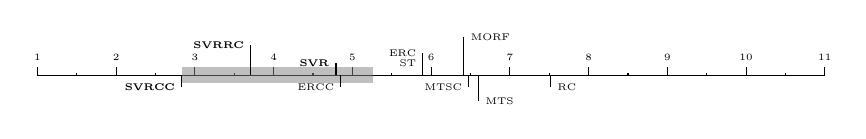
\begin{tikzpicture}
 %axis
 \draw (1,0) -- (11,0);
 \foreach \x in {1,2,3,4,5,6,7,8,9,10,11} {
  \draw (\x, 0) -- ++(0,.1) node [above,scale=0.7] {\tiny \x};
  \ifthenelse{\x < 11}{\draw (\x+.5, 0) -- ++(0,.03);}{}
 }
 % coordinates
 \coordinate (c0) at (2.8333,0);
 \coordinate (c1) at (3.7083,0);
 \coordinate (c2) at (4.7917,0);
 \coordinate (c3) at (4.8542,0);
 \coordinate (c4) at (5.8958,0);
 \coordinate (c5) at (7.5208,0);
 \coordinate (c6) at (6.4792,0);
 \coordinate (c7) at (6.6042,0);
 \coordinate (c8) at (5.8958,0);
 \coordinate (c9) at (6.4167,0);

 % labels
 \node (l0) at (c0) [below left=.025cm and 0cm, align=right, scale=0.7] {\tiny \textbf{SVRCC}};
 \node (l1) at (c1) [above left=.25cm and 0cm, align=right, scale=0.7] {\tiny \textbf{SVRRC}};
 \node (l2) at (c2) [above left=.025cm and 0cm, align=right, scale=0.7] {\tiny \textbf{SVR}};
 \node (l3) at (c3) [below left=.025cm and 0cm, align=left, scale=0.7] {\tiny ERCC};
 \node (l4) at (c4) [above left=.15cm and 0cm, align=right, scale=0.7] {\tiny ERC};
 \node (l5) at (c5) [below right=.025cm and 0cm, align=left, scale=0.7] {\tiny RC};
 \node (l6) at (c6) [below left=.025cm and 0cm, align=right, scale=0.7] {\tiny MTSC};
 \node (l7) at (c7) [below right=.2cm and 0cm, align=left, scale=0.7] {\tiny MTS};
 \node (l8) at (c8) [above left=.025cm and 0cm, align=right, scale=0.7] {\tiny ST};
 \node (l9) at (c9) [above right=.35cm and 0cm, align=right, scale=0.7] {\tiny MORF};

 % CD = 1.4845
 \fill[fill=gray,fill opacity=0.5] (2.8333,-0.1) rectangle (5.2569,0.1);
 
 % connectors
 \foreach \x in {0,...,9} {
  \draw (l\x) -| (c\x);
 };
\end{tikzpicture}}\vspace{-1em}
\captionof{figure}{Bonferroni-Dunn test for aCC}\label{fig:BonfDunnACC}\vspace{-1.3em}
\captionof{table}{Wilcoxon, Nemenyi, and Holm tests for aCC}\label{tab:statacc}
\vspace{-1.3em}
\scriptsize
\resizebox{0.95\textwidth}{!}{\begin{tabular}{lccccc}
\noalign{\smallskip}\hline\noalign{\smallskip}
SVRCC vs. & Wilcoxon $R^{+}$ & Wilcoxon $R^{-}$ & Wilcoxon $p$-value & Nemenyi $p$-value & Holm $p$-value \\ 
\noalign{\smallskip}\hline\noalign{\smallskip}
MORF & 224.0 & 76.0 & $3.4E^{-2}$ & $4.1E^{-5}$& $8.3E^{-3}$ \\
ST & 239.0 & 61.0 & $9.6E^{-3}$ & $4.6E^{-4}$ & $1.3E^{-2}$ \\ 
MTS & 242.0 & 58.0 & $7.2E^{-3}$ & $1.6E^{-5}$ & $6.3E^{-3}$ \\ 
MTSC & 238.0 & 62.0 & $1.1E^{-2}$ & $3.0E^{-5}$ & $7.1E^{-3}$ \\ 
RC & 250.0 & 50.0 & $3.1E^{-3}$ & 0.0000 & $5.6E^{-3}$ \\
ERC & 229.0 & 71.0 & $2.3E^{-2}$ & $4.6E^{-4}$ & $1.0E^{-2}$ \\ 
ERCC & 221.0 & 79.0 & $4.3E^{-2}$ & $2.1E^{-2}$ & $1.7E^{-2}$ \\ 
SVR & 297.0 & 3.00 & $6.0E^{-7}$ & $2.5E^{-2}$ & $2.5E^{-2}$ \\ 
SVRRC & 266.5 & 33.5 & $4.0E^{-4}$ & $3.2E^{-1}$ & $5.0E^{-2}$ \\ 
\noalign{\smallskip}\hline\noalign{\smallskip}
\end{tabular}}
\end{table}
Table~{\ref{tab:mtraccResults}} shows that our proposed methods perform the best on $15$ out of the $24$ datasets. Specifically, the maximum correlation chain method, SVRCC, performs the best on $11$, which is better than the total number of datasets the competing methods performed better at ($9$). The Iman-Davenport statistic, distributed according to the F-distribution with 9 and 207 degrees of freedom is $6.72$, with a $p$-value of $1.9E^{-8}$ which is significantly less than $0.01$, implying a statistical confidence larger than $99\%$. Therefore, we can conclude that there exist statistically significant differences between the aCC results of the algorithms.

Figure~{\ref{fig:BonfDunnACC}} shows the mean rank values of each algorithm along with the critical difference value, $2.4236$, for $\alpha = 0.05$. The algorithms that are to the right of the critical difference rectangle are the ones with significantly different results. Therefore, the $6$ out of $10$ algorithms beyond the critical difference perform significantly worse than our control algorithm, SVRCC. Table~{\ref{tab:statacc}} provides complementary analysis of the results. According to the Wilcoxon test, SVRCC is shown to have significantly better performance over all algorithms with $p$-value $< 0.05$. The Nemenyi and Holm tests show that SVRCC performs significantly better than $6$ out of the $9$ algorithms with $p$-value $\leq 5.6E^{-3}$ and $\leq 1.7E^{-2}$, respectively. The exact confidence for algorithm SVRCC against all others is $0.95$.

\begin{table}[b!]
\centering \small
\caption{Mean Square Error (MSE) for MT regressors}\label{tab:mseResults}
\resizebox{0.95\textwidth}{!}{\begin{tabular}{l@{\extracolsep{\fill}}ccccccccccc}
\noalign{\smallskip}\hline\noalign{\smallskip}
Datasets &MORF &ST &MTS &MTSC &RC &ERC &ERCC &SVR &SVRRC &SVRCC \\
\noalign{\smallskip}\hline\noalign{\smallskip}
Slump &1.4388 &1.4161 &1.3667 &1.4414 &1.4602 &1.4727 &1.4183 &1.2991 &1.1726 &\textbf{1.1614} &  \\
Polymer &1.6718 &1.8120 &1.5446 &1.6726 &1.8259 &1.9999 &1.6873 &1.1874 &1.1068 &\textbf{1.0796} &  \\
Andro &1.4930 &2.1467 &1.4714 &1.7525 &2.2603 &2.0812 &1.8707 &1.5406 &1.2847 &\textbf{1.2187} &  \\
EDM &\textbf{0.8342} &0.9373 &0.9352 &0.9418 &0.9389 &0.9326 &0.9393 &0.9092 &0.8650 &0.8817 &  \\
Solar Flare 1 &3.3458 &3.1196 &3.1193 &3.0524 &3.0357 &3.0381 &3.0594 &\textbf{2.9912} &3.0176 &3.0129 &  \\
Jura &1.0973 &1.0595 &1.0732 &1.0695 &1.0744 &1.0694 &1.0632 &1.1167 &1.0435 &\textbf{1.0315} &  \\
Enb &0.0381 &0.0361 &0.0407 &0.0377 &0.0452 &0.0403 &0.0343 &0.0255 &0.0216 &\textbf{0.0214} &  \\
Solar Flare 2 &2.9619 &2.8532 &\textbf{2.7732} &2.8282 &2.8510 &2.8273 &2.8110 &2.9518 &2.9204 &2.8713 &  \\
Wisconsin Cancer &1.7666 &1.7155 &1.7156 &1.7256 &\textbf{1.7119} &1.7146 &1.7195 &1.8171 &1.7915 &1.7692 &  \\
California Housing &0.8665 &0.8221 &0.9642 &0.8673 &1.0125 &0.8952 &0.7513 &0.7477 &0.6987 &\textbf{0.6726} &  \\
Stock &0.0841 &0.1039 &0.0990 &0.1008 &0.0998 &0.0987 &0.0949 &0.0578 &0.0596 &\textbf{0.0554} &  \\
SCPF &\textbf{2.2244} &2.3173 &2.3661 &2.3517 &2.3923 &2.3025 &2.3295 &2.2960 &2.2510 &2.3179 &  \\
Puma8NH &1.9678 &2.1133 &2.0989 &2.2024 &2.1413 &2.1473 &2.1467 &\textbf{1.8242} &1.8728 &1.8299 &  \\
Friedman &5.4573 &5.3357 &5.3478 &5.3260 &5.3482 &5.3253 &5.3210 &5.3038 &5.2942 &\textbf{5.2812} &  \\
Puma32H &5.3419 &\textbf{4.9499} &4.9627 &5.0405 &4.9905 &4.9662 &4.9805 &5.2711 &5.2749 &5.1306 &  \\
Water Quality &\textbf{11.3143} &11.5621 &11.6276 &11.5931 &11.6495 &11.6022 &11.5004 &12.2974 &12.2042 &12.0593 &  \\
M5SPEC &1.0081 &0.8754 &1.0336 &0.9421 &0.8847 &0.8824 &0.8903 &0.2578 &0.2597 &\textbf{0.2575} &  \\
MP5SPEC &1.1483 &0.9817 &1.1953 &0.9970 &0.9886 &0.9880 &0.9882 &0.2261 &\textbf{0.1979} &0.2136 &  \\
MP6SPEC &1.1626 &0.9928 &1.1906 &0.9992 &1.0115 &1.0045 &0.9905 &0.2926 &\textbf{0.2903} &0.2954 &  \\
ATP7d &1.7859 &1.7348 &\textbf{1.6435} &1.6460 &1.8521 &1.7888 &1.6739 &1.7820 &1.7433 &1.7098 &  \\
OES97 &4.6331 &4.8340 &4.8379 &4.8082 &4.8573 &4.8591 &4.8187 &3.1440 &3.0633 &\textbf{3.0499} &  \\
Osales &7.3631 &6.6850 &\textbf{5.8848} &6.0850 &7.8575 &6.4746 &5.9155 &7.0727 &7.3153 &7.1374 &  \\
ATP1d &1.0589 &0.9056 &0.9053 &0.8982 &0.9125 &\textbf{0.8783} &0.9004 &0.9091 &0.8837 &0.8922 &  \\
OES10 &3.6471 &3.8931 &3.8952 &3.8909 &3.9031 &3.9063 &3.8869 &2.2623 &2.1608 &\textbf{2.1320} &  \\
\noalign{\smallskip}\hline\noalign{\smallskip}
Average &2.6546 &2.6334 &2.5872 &2.5946 &2.7127 &2.6373 &2.5747 &2.3993 &2.3664 &\textbf{2.3368} &  \\
Ranks &6.5833 &5.6667 &6.0833 &6.2500 &7.8333 &6.1250 &5.1250 &4.6667 &3.6250 &\textbf{3.0417} &  \\
\noalign{\smallskip}\hline
\end{tabular}}
\centering \small
\resizebox{0.95\textwidth}{!}{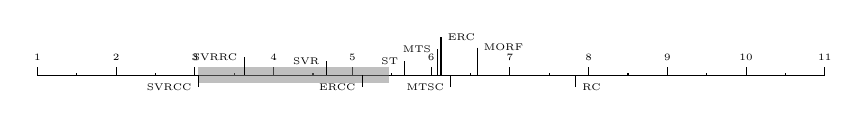
\begin{tikzpicture}
 %axis
 \draw (1,0) -- (11,0);
 \foreach \x in {1,2,3,4,5,6,7,8,9,10,11} {
  \draw (\x, 0) -- ++(0,.1) node [above,scale=0.7] {\tiny \x};
  \ifthenelse{\x < 11}{\draw (\x+.5, 0) -- ++(0,.03);}{}
 }
 % coordinates
 \coordinate (c0) at (3.0417,0);
 \coordinate (c1) at (3.6250,0);
 \coordinate (c2) at (4.6667,0);
 \coordinate (c3) at (5.1250,0);
 \coordinate (c4) at (6.1250,0);
 \coordinate (c5) at (7.8333,0);
 \coordinate (c6) at (6.2500,0);
 \coordinate (c7) at (6.0833,0);
 \coordinate (c8) at (5.6667,0);
 \coordinate (c9) at (6.5833,0);

 % labels
 \node (l0) at (c0) [below left=.025cm and 0cm, align=right,scale=0.7] {\tiny SVRCC};
 \node (l1) at (c1) [above left=.1cm and 0cm, align=right,scale=0.7] {\tiny SVRRC};
 \node (l2) at (c2) [above left=.05cm and 0cm, align=right,scale=0.7] {\tiny SVR};
 \node (l3) at (c3) [below left=.025cm and 0cm, align=left,scale=0.7] {\tiny ERCC};
 \node (l4) at (c4) [above right=.35cm and 0cm, align=right,scale=0.7] {\tiny ERC};
 \node (l5) at (c5) [below right=.025cm and 0cm, align=left,scale=0.7] {\tiny RC};
 \node (l6) at (c6) [below left=.025cm and 0cm, align=right,scale=0.7] {\tiny MTSC};
 \node (l7) at (c7) [above left=.2cm and 0cm, align=left,scale=0.7] {\tiny MTS};
 \node (l8) at (c8) [above left=.05cm and 0cm, align=right,scale=0.7] {\tiny ST};
 \node (l9) at (c9) [above right=.22cm and 0cm, align=right,scale=0.7] {\tiny MORF};

 % CD = 1.4845
 \fill[fill=gray,fill opacity=0.5] (3.0417,-0.1) rectangle (5.4653,0.1);
 
 % connectors
 \foreach \x in {0,...,9} {
  \draw (l\x) -| (c\x);
 };
\end{tikzpicture}}\vspace{-1em}
\captionof{figure}{Bonferroni-Dunn test for MSE}\label{fig:BonfDunnMSE}\vspace{-1.5em}
\captionof{table}{Wilcoxon, Nemenyi, and Holm tests for MSE}\label{tab:statmse}
\scriptsize
\resizebox{0.95\textwidth}{!}{\begin{tabular}{lccccc}
\noalign{\smallskip}\hline\noalign{\smallskip}
SVRCC vs. & Wilcoxon $R^{+}$ & Wilcoxon $R^{-}$ & Wilcoxon $p$-value & Nemenyi $p$-value & Holm $p$-value \\ 
\noalign{\smallskip}\hline\noalign{\smallskip}
MORF & 268.0 & 32.0 & $3.2E^{-4}$ & $5.1E^{-5}$ & $6.3E^{-3}$ \\
ST & 241.0 & 59.0 & $7.9E^{-3}$ & $2.7E^{-3}$ & $1.3E^{-2}$ \\
MTS & 224.0 & 76.0 & $3.4E^{-2}$ & $5.0E^{-4}$ & $1.0E^{-2}$ \\
MTSC & 226.0 & 74.0 & $2.9E^{-2}$ & $2.4E^{-4}$ & $7.1E^{-3}$ \\ 
RC & 263.0 & 37.0 & $6.5E^{-4}$ & 0.0000 & $5.6E^{-3}$ \\  
ERC & 234.0 & 66.0 & $1.5E^{-2}$ & $4.2E^{-4}$ & $8.3E^{-3}$ \\
ERCC & 224.0 & 76.0 & $3.4E^{-2}$ & $1.7E^{-2}$ & $1.7E^{-2}$ \\
SVR & 262.0 & 38.0 & $7.4E^{-4}$ & $6.3E^{-2}$ & $2.5E^{-2}$ \\ 
SVRRC & 245.0 & 55.0 & $5.3E^{-3}$ & $5.1E^{-1}$ & $5.0E^{-2}$\\ 
\noalign{\smallskip}\hline\noalign{\smallskip}
\end{tabular}}
\end{table}
\subsection{Mean Square Error}\label{subsec:mse}
Table~{\ref{tab:mseResults}} shows that our proposed methods perform the best on $15$ out of the $24$ datasets. In this case, SVRCC also performs the best on $11$ versus the $9$ that the competing methods performed better at. The Iman-Davenport statistic, distributed according to the F-distribution with $9$ and $207$ degrees of freedom is $6.57$, with a $p$-value of $3.1E^{-8}$, implying statistically significant differences among the MSE results.

Figure~{\ref{fig:BonfDunnMSE}} shows the mean rank values of each algorithm along with the critical difference value, $2.4236$, for $\alpha = 0.05$. According to the critical difference bar, there are $6$ out of $10$ algorithms beyond that perform significantly worse than our control algorithm, SVRCC. According to the Wilcoxon test, shown in Table~{\ref{tab:statmse}}, SVRCC is shown to have significantly better performance over all algorithms with $p$-value $< 0.05$. The Nemenyi and Holm tests show that SVRCC performs significantly better than $6$ out of the $9$ algorithms with $p$-values $\leq 5.6E^{-3}$ and $\leq 1.7E^{-2}$ respectively, and has an exact confidence of $0.95$ against all others.

\subsection{Average Root Mean Square Error}\label{subsec:armse}
Table~{\ref{tab:armseresults}} shows that our proposed methods perform the best on $18$ out of the $24$ datasets. In this case, SVRCC performs the best on $15$ versus the $6$ that the methods compared performed better at. The Iman-Davenport statistic is $7.6$, with a $p$-value of $1.3E^{-9}$, implying statistically significant differences in the aRMSE results.

Figure~{\ref{fig:BonfDunnaRMSE}} shows the mean rank values of each algorithm along with the critical difference value, $2.4236$, for $\alpha = 0.05$. According to the critical difference bar, there are $7$ out of $10$ algorithms that perform significantly worse than our control algorithm, SVRCC.

According to the Wilcoxon test, shown in Table~{\ref{tab:statarmse}}, SVRCC is shown to have significantly better performance over all algorithms with $p$-value $< 0.01$. The Nemenyi test shows that SVRCC performs significantly better than $7$ out of the $9$ algorithms with $p$-value $\leq 5.6E^{-3}$, while the stricter Holm test shows that it performs significantly better than $8$ out of the $9$ algorithms with $p$-value $\leq 0.05$.
\begin{table}[t!]
\centering \small
\caption{Average Root Mean Square Error (aRMSE) for MT regressors}\label{tab:armseresults}
\resizebox{0.95\textwidth}{!}{\begin{tabular}{l@{\extracolsep{\fill}}ccccccccccc}
\noalign{\smallskip}\hline\noalign{\smallskip}
Datasets &MORF &ST &MTS &MTSC &RC &ERC &ERCC &SVR &SVRRC &SVRCC \\
\noalign{\smallskip}\hline\noalign{\smallskip}
Slump &0.6711 &0.6652 &0.6456 &0.6699 &0.6787 &0.6793 &0.6649 &0.5561 &0.5345 &\textbf{0.5337} &  \\
Polymer &0.5277 &0.5409 &0.5042 &0.5336 &0.5536 &0.5803 &0.5319 &0.4403 &0.4062 &\textbf{0.4060} &  \\
Andro &0.4649 &0.5420 &0.4414 &0.4871 &0.5390 &0.5317 &0.5039 &0.4326 &0.4061 &\textbf{0.3989} &  \\
EDM &0.6372 &0.6715 &0.6705 &0.6729 &0.6722 &0.6704 &0.6721 &0.6449 &0.6411 &\textbf{0.6366} &  \\
Solar Flare 1 &0.9777 &0.9274 &0.9271 &0.9089 &0.8921 &0.9016 &0.9121 &0.8856 &0.8844 &\textbf{0.8801} &  \\
Jura &0.5800 &0.5686 &0.5720 &0.5706 &0.5726 &0.5712 &0.5693 &0.5794 &0.5687 &\textbf{0.5622} &  \\
Enb &0.1212 &0.1166 &0.1237 &0.1214 &0.1272 &0.1253 &0.1140 &0.0981 &0.0914 &\textbf{0.0903} &  \\
Solar Flare 2 &0.8725 &0.8420 &\textbf{0.8127} &0.8305 &0.8313 &0.8300 &0.8304 &0.8418 &0.8349 &0.8345 &  \\
Wisconsin Cancer &0.9290 &0.9163 &0.9158 &0.9187 &\textbf{0.9153} &0.9160 &0.9173 &0.9422 &0.9362 &0.9306 &  \\
California Housing &0.6541 &0.6366 &0.6889 &0.6530 &0.7053 &0.6632 &0.6079 &0.6038 &0.5859 &\textbf{0.5755} &  \\
Stock &0.1643 &0.1830 &0.1774 &0.1790 &0.1790 &0.1777 &0.1739 &0.1357 &0.1329 &\textbf{0.1308} &  \\
SCPF &0.7113 &0.7235 &0.7342 &0.7255 &0.7285 &0.7143 &0.7227 &0.7155 &0.7081 &\textbf{0.7048} &  \\
Puma8NH &0.7855 &0.8139 &0.8114 &0.8307 &0.8196 &0.8202 &0.8203 &\textbf{0.7650} &0.7740 &0.7671 &  \\
Friedman &0.9382 &0.9203 &0.9219 &0.9199 &0.9219 &0.9197 &0.9193 &0.9203 &0.9195 &\textbf{0.9183} &  \\
Puma32H &0.9395 &\textbf{0.8700} &0.8713 &0.8778 &0.8739 &0.8716 &0.8727 &0.9353 &0.9356 &0.9331 &  \\
Water Quality &\textbf{0.8921} &0.9015 &0.9041 &0.9025 &0.9051 &0.9030 &0.8990 &0.9284 &0.9293 &0.9271 &  \\
M5SPEC &0.5707 &0.5324 &0.5761 &0.5515 &0.5347 &0.5339 &0.5376 &0.2745 &0.2744 &\textbf{0.2740} &  \\
MP5SPEC &0.5315 &0.4914 &0.5426 &0.4947 &0.4930 &0.4928 &0.4928 &0.2337 &\textbf{0.2176} &0.2177 &  \\
MP6SPEC &0.5344 &0.4939 &0.5416 &0.4943 &0.4982 &0.4967 &0.4927 &0.2627 &\textbf{0.2460} &0.2497 &  \\
ATP7d &0.5216 &0.4956 &\textbf{0.4752} &0.4765 &0.5194 &0.5024 &0.4824 &0.5141 &0.5066 &0.5018 &  \\
OES97 &0.4652 &0.4634 &0.4635 &0.4622 &0.4643 &0.4644 &0.4627 &0.3794 &0.3768 &\textbf{0.3749} &  \\
Osales &0.7190 &0.6912 &\textbf{0.6496} &0.6615 &0.7591 &0.6772 &0.6515 &0.7212 &0.7343 &0.7121 &  \\
ATP1d &0.4053 &0.3608 &0.3587 &0.3591 &0.3653 &0.3562 &0.3596 &0.3693 &0.3638 &\textbf{0.3507} &  \\
OES10 &0.3954 &0.3896 &0.3897 &0.3892 &0.3901 &0.3903 &0.3889 &0.3085 &0.3039 &\textbf{0.3038} &  \\
\noalign{\smallskip}\hline\noalign{\smallskip}
Average &0.6254 &0.6149 &0.6133 &0.6121 &0.6225 &0.6162 &0.6083 &0.5620 &0.5547 &\textbf{0.5506} &  \\
Ranks &7.3333 &5.7708 &5.8125 &6.0625 &7.6250 &6.0208 &4.8542 &5.0625 &3.9167 &\textbf{2.5417} &  \\
\noalign{\smallskip}\hline
\end{tabular}}
\centering \small
\resizebox{0.95\textwidth}{!}{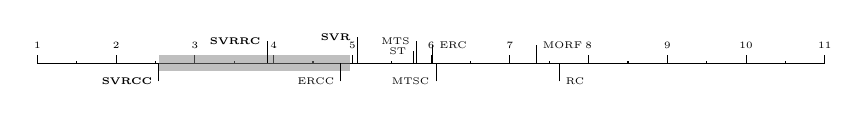
\begin{tikzpicture}
 %axis
 \draw (1,0) -- (11,0);
 \foreach \x in {1,2,3,4,5,6,7,8,9,10,11} {
  \draw (\x, 0) -- ++(0,.1) node [above,scale=0.7] {\tiny \x};
  \ifthenelse{\x < 11}{\draw (\x+.5, 0) -- ++(0,.03);}{}
 }
 % coordinates
 \coordinate (c0) at (2.5417,0);
 \coordinate (c1) at (3.9167,0);
 \coordinate (c2) at (5.0625,0);
 \coordinate (c3) at (4.8542,0);
 \coordinate (c4) at (6.0208,0);
 \coordinate (c5) at (7.6250,0);
 \coordinate (c6) at (6.0625,0);
 \coordinate (c7) at (5.8125,0);
 \coordinate (c8) at (5.7708,0);
 \coordinate (c9) at (7.3333,0);

 % labels
 \node (l0) at (c0) [below left=.1cm and 0cm, align=right,scale=0.7] {\tiny \textbf{SVRCC}};
 \node (l1) at (c1) [above left=.15cm and 0cm, align=right,scale=0.7] {\tiny \textbf{SVRRC}};
 \node (l2) at (c2) [above left=.2cm and 0cm, align=right,scale=0.7] {\tiny \textbf{SVR}};
 \node (l3) at (c3) [below left=.1cm and 0cm, align=left,scale=0.7] {\tiny ERCC};
 \node (l4) at (c4) [above right=.1cm and 0cm, align=right,scale=0.7] {\tiny ERC};
 \node (l5) at (c5) [below right=.1cm and 0cm, align=left,scale=0.7] {\tiny RC};
 \node (l6) at (c6) [below left=.1cm and 0cm, align=right,scale=0.7] {\tiny MTSC};
 \node (l7) at (c7) [above left=.15cm and 0cm, align=left,scale=0.7] {\tiny MTS};
 \node (l8) at (c8) [above left=.025cm and 0cm, align=right,scale=0.7] {\tiny ST};
 \node (l9) at (c9) [above right=.1cm and 0cm, align=right,scale=0.7] {\tiny MORF};

 % CD = 1.4845
 \fill[fill=gray,fill opacity=0.5] (2.5417,-0.1) rectangle (4.9653,0.1);
 
 % connectors
 \foreach \x in {0,...,9} {
  \draw (l\x) -| (c\x);
 };
\end{tikzpicture}}\vspace{-1em}
\captionof{figure}{Bonferroni-Dunn test for aRMSE}\label{fig:BonfDunnaRMSE}\vspace{-1.5em}
\captionof{table}{Wilcoxon, Nemenyi, and Holm tests for aRMSE}\label{tab:statarmse}
\scriptsize
\resizebox{0.95\textwidth}{!}{\begin{tabular}{lccccc}
\noalign{\smallskip}\hline\noalign{\smallskip}
SVRCC vs. & Wilcoxon $R^{+}$ & Wilcoxon $R^{-}$ & Wilcoxon $p$-value & Nemenyi $p$-value & Holm $p$-value \\ 
\noalign{\smallskip}\hline\noalign{\smallskip}
MORF & 286.0 & 14.0 & $1.3E^{-5}$ & 0.0000 & $6.3E^{-3}$ \\
ST & 259.0 & 41.0 & $1.1E^{-3}$ & $2.2E^{-4}$ & $1.3E^{-2}$ \\
MTS & 247.0 & 53.0 & $4.3E^{-3}$ & $1.8E^{-5}$ & $1.0E^{-2}$ \\ 
MTSC & 251.0 & 49.0 & $2.8E^{-3}$ & $5.6E^{-5}$ & $7.1E^{-3}$ \\
RC & 270.0 & 30.0 & $2.4E^{-4}$ & 0.0000 & $5.6E^{-3}$ \\ 
ERC & 255.0 & 45.0 & $1.8E^{-3}$ & $6.9E^{-5}$ & $8.3E^{-3}$ \\
ERCC & 246.0 & 54.0 & $4.8E^{-3}$ & $8.2E^{-3}$ & $2.5E^{-2}$ \\
SVR & 296.0 & 4.00 & $8.3E^{-7}$ & $3.9E^{-3}$ & $1.7E^{-2}$ \\
SVRRC & 284.0 & 16.0 & $2.0E^{-5}$ & $1.2E^{-1}$ & $5.0E^{-2}$ \\
\noalign{\smallskip}\hline\noalign{\smallskip}
\end{tabular}}
\end{table}

\subsection{Average Relative Root Mean Square Error}\label{subsec:arrmse}
\begin{table}[b!]
\centering \small
\caption{Average Relative Root Mean Square Error (aRRMSE) for MT regressors}\label{tab:arrmseresults}
\resizebox{0.95\textwidth}{!}{\begin{tabular}{l@{\extracolsep{\fill}}ccccccccccc}
\noalign{\smallskip}\hline\noalign{\smallskip}
Datasets &MORF &ST &MTS &MTSC &RC &ERC &ERCC &SVR &SVRRC &SVRCC \\
\noalign{\smallskip}\hline\noalign{\smallskip}
Slump &0.6939 &0.6886 &0.6690 &0.6938 &0.7019 &0.7022 &0.6886 &0.5765 &\textbf{0.5545} &0.5560 &  \\
Polymer &0.6159 &0.5971 &0.5778 &0.6493 &0.6270 &0.6544 &0.6131 &0.5573 &0.5253 &\textbf{0.5116} &  \\
Andro &0.5097 &0.5979 &0.5155 &0.5633 &0.5924 &0.5885 &0.5666 &0.4856 &0.4651 &\textbf{0.4455} &  \\
EDM &0.7337 &0.7442 &0.7413 &0.7446 &0.7449 &0.7452 &0.7443 &0.7058 &0.7070 &\textbf{0.6978} &  \\
Solar Flare 1 &1.3046 &1.1357 &1.1168 &1.0758 &0.9951 &1.0457 &1.0887 &0.9917 &0.9455 &\textbf{0.9320} &  \\
Jura &0.5969 &0.5874 &0.5906 &0.5892 &0.5910 &0.5896 &0.5880 &0.5952 &\textbf{0.5764} &0.5885 &  \\
Enb &0.1210 &0.1165 &0.1231 &0.1211 &0.1268 &0.1250 &0.1139 &0.0977 &0.0910 &\textbf{0.0899} &  \\
Solar Flare 2 &1.4167 &1.1503 &\textbf{0.9483} &1.0840 &1.0092 &1.0522 &1.0928 &1.0385 &1.0253 &1.0298 &  \\
Wisconsin Cancer &0.9413 &0.9314 &0.9308 &0.9336 &\textbf{0.9305} &0.9313 &0.9323 &0.9555 &0.9483 &0.9427 &  \\
California Housing &0.6611 &0.6447 &0.6974 &0.6630 &0.7131 &0.6690 &0.6146 &0.6130 &0.5945 &\textbf{0.5852} &  \\
Stock &0.1653 &0.1844 &0.1787 &0.1803 &0.1802 &0.1789 &0.1752 &0.1364 &\textbf{0.1337} &0.1388 &  \\
SCPF &0.8273 &0.8348 &0.8436 &0.8308 &0.8263 &0.8105 &0.8290 &0.8164 &0.8037 &\textbf{0.8013} &  \\
Puma8NH &0.7858 &0.8142 &0.8118 &0.8311 &0.8199 &0.8205 &0.8207 &\textbf{0.7655} &0.7744 &0.7676 &  \\
Friedman &0.9394 &0.9214 &0.9231 &0.9210 &0.9231 &0.9209 &0.9204 &0.9218 &0.9208 &\textbf{0.9196} &  \\
Puma32H &0.9406 &\textbf{0.8713} &0.8727 &0.8791 &0.8752 &0.8729 &0.8740 &0.9364 &0.9367 &0.9319 &  \\
Water Quality &\textbf{0.8994} &0.9085 &0.9109 &0.9093 &0.9121 &0.9097 &0.9057 &0.9343 &0.9310 &0.9045 &  \\
M5SPEC &0.5910 &0.5523 &0.5974 &0.5671 &0.5552 &0.5542 &0.5558 &0.2951 &0.2935 &\textbf{0.2925} &  \\
MP5SPEC &0.5522 &0.5120 &0.5683 &0.5133 &0.5145 &0.5143 &0.5119 &0.2484 &\textbf{0.2323} &0.2358 &  \\
MP6SPEC &0.5553 &0.5152 &0.5686 &0.5119 &0.5198 &0.5187 &0.5109 &0.2850 &0.2669 &\textbf{0.2623} &  \\
ATP7d &0.5563 &0.5308 &\textbf{0.5141} &0.5142 &0.5558 &0.5397 &0.5182 &0.5455 &0.5371 &0.5342 &  \\
OES97 &0.5490 &0.5230 &0.5229 &0.5217 &0.5239 &0.5237 &0.5222 &0.4641 &\textbf{0.4618} &0.4635 &  \\
Osales &0.7596 &0.7471 &\textbf{0.7086} &0.7268 &0.8318 &0.7258 &0.7101 &0.7924 &0.7924 &0.7811 &  \\
ATP1d &0.4173 &0.3732 &0.3733 &0.3712 &0.3790 &\textbf{0.3696} &0.3721 &0.3773 &0.3707 &0.3775 &  \\
OES10 &0.4518 &0.4174 &0.4176 &0.4171 &0.4178 &0.4180 &0.4166 &0.3570 &0.3555 &\textbf{0.3538} &  \\
\noalign{\smallskip}\hline\noalign{\smallskip}
Average &0.6910 &0.6625 &0.6551 &0.6589 &0.6611 &0.6575 &0.6536 &0.6039 &0.5935 &\textbf{0.5893} &  \\
Ranks &7.5000 &5.7708 &5.9375 &6.1667 &7.4375 &6.3750 &4.9792 &4.7708 &3.2708 &\textbf{2.7917} &  \\
\noalign{\smallskip}\hline
\end{tabular}}
\centering \small
\resizebox{0.95\textwidth}{!}{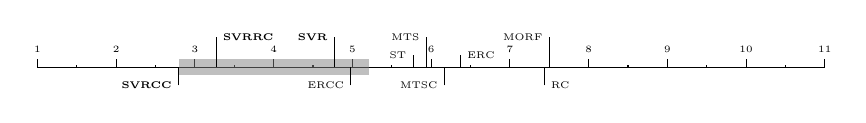
\begin{tikzpicture}
 %axis
 \draw (1,0) -- (11,0);
 \foreach \x in {1,2,3,4,5,6,7,8,9,10,11} {
  \draw (\x, 0) -- ++(0,.1) node [above,scale=0.7] {\tiny \x};
  \ifthenelse{\x < 11}{\draw (\x+.5, 0) -- ++(0,.03);}{}
 }
 % coordinates
 \coordinate (c0) at (2.7917,0);
 \coordinate (c1) at (3.2708,0);
 \coordinate (c2) at (4.7708,0);
 \coordinate (c3) at (4.9792,0);
 \coordinate (c4) at (6.3750,0);
 \coordinate (c5) at (7.4375,0);
 \coordinate (c6) at (6.1667,0);
 \coordinate (c7) at (5.9375,0);
 \coordinate (c8) at (5.7708,0);
 \coordinate (c9) at (7.5000,0);

 % labels
 \node (l0) at (c0) [below left=.1cm and 0cm, align=right,scale=0.7] {\tiny \textbf{SVRCC}};
 \node (l1) at (c1) [above right=.25cm and 0cm, align=right,scale=0.7] {\tiny \textbf{SVRRC}};
 \node (l2) at (c2) [above left=.25cm and 0cm, align=right,scale=0.7] {\tiny \textbf{SVR}};
 \node (l3) at (c3) [below left=.1cm and 0cm, align=left,scale=0.7] {\tiny ERCC};
 \node (l4) at (c4) [above right=.025cm and 0cm, align=right,scale=0.7] {\tiny ERC};
 \node (l5) at (c5) [below right=.1cm and 0cm, align=left,scale=0.7] {\tiny RC};
 \node (l6) at (c6) [below left=.1cm and 0cm, align=right,scale=0.7] {\tiny MTSC};
 \node (l7) at (c7) [above left=.25cm and 0cm, align=left,scale=0.7] {\tiny MTS};
 \node (l8) at (c8) [above left=.025cm and 0cm, align=right,scale=0.7] {\tiny ST};
 \node (l9) at (c9) [above left=.25cm and 0cm, align=right,scale=0.7] {\tiny MORF};

 % CD = 1.4845
 \fill[fill=gray,fill opacity=0.5] (2.7917,-0.1) rectangle (5.2153,0.1);
 
 % connectors
 \foreach \x in {0,...,9} {
  \draw (l\x) -| (c\x);
 };
\end{tikzpicture}}\vspace{-1em}
\captionof{figure}{Bonferroni-Dunn test for aRRMSE}\label{fig:BonfDunnaRRMSE}\vspace{-1.5em}
\captionof{table}{Wilcoxon, Nemenyi, and Holm tests for aRRMSE}\label{tab:statarrmse}
\scriptsize
\resizebox{0.95\textwidth}{!}{\begin{tabular}{lccccc}
\noalign{\smallskip}\hline\noalign{\smallskip}
SVRCC vs. & Wilcoxon $R^{+}$ & Wilcoxon $R^{-}$ & Wilcoxon $p$-value & Nemenyi $p$-value & Holm $p$-value \\ 
\noalign{\smallskip}\hline\noalign{\smallskip}
MORF & 290.0 & 10.0 & $5.1E^{-6}$ & $0.0000$ & $5.6E^{-3}$ \\  
ST & 261.0 & 39.0 & $8.5E^{-4}$ & $6.5E^{-4}$ & $1.3E^{-2}$\\
MTS & 239.0 & 61.0 & $9.6E^{-3}$ & $3.2E^{-3}$ & $1.0E^{-2}$\\ 
MTSC & 261.0 & 39.0 & $8.5E^{-4}$ & $1.1E^{-3}$ & $8.3E^{-3}$\\  
RC & 275.0 & 25.0 & $1.1E^{-4}$ & 0.0000 & $6.3E^{-3}$ \\
ERC & 261.0 & 39.0 & $8.5E^{-4}$ & $4.1E^{-5}$ & $7.1E^{-3}$\\ 
ERCC & 254.0 & 46.0 & $2.0E^{-3}$ & $1.2E^{-2}$ & $1.7E^{-2}$\\
SVR & 291.0 & 9.00 & $3.9E^{-6}$ & $2.4E^{-2}$ & $2.5E^{-2}$\\
SVRRC & 222.5 & 77.5 & $3.8E^{-2}$ & $5.8E^{-1}$ & $5.0E^{-2}$ \\ 
\noalign{\smallskip}\hline\noalign{\smallskip}
\end{tabular}}
\end{table}
Table~{\ref{tab:arrmseresults}} shows that our proposed methods perform the best on $16$ out of the $24$ datasets. In this case, SVRCC performs the best on $11$ versus the $6$ that the competing methods performed better at. The Iman-Davenport statistic is $8.54$, with a $p$-value of $7.6E^{-11}$.

Figure~{\ref{fig:BonfDunnaRRMSE}} shows the mean rank values of each algorithm along with the critical difference value, $2.4236$, for $\alpha = 0.05$. According to the critical difference bar, there are $6$ out of $10$ algorithms beyond that perform significantly worse than our control algorithm, SVRCC.

According to the Wilcoxon test, shown in Table~{\ref{tab:statarrmse}}, SVRCC is shown to have significantly better performance over all algorithms with $p$-value $< 0.05$, and $8$ out of the $9$ algorithms for $p$-value $< 0.01$. The Nemenyi test shows that SVRCC performs significantly better than $6$ out of the $9$ algorithms with $p$-value $\leq 5.6E^{-3}$, and the Holm test shows its performance is significantly better than $8$ out of the $9$ algorithms with $p$-value $\leq 0.05$.

\subsection{Run Time}\label{subsec:time}
\begin{table}[t!]
\centering \small
\caption{Run Time (seconds) for MT regressors}\label{tab:timeresults}
\resizebox{0.95\textwidth}{!}{\begin{tabular}{l@{\extracolsep{\fill}}rrrrrrrrrrr}
\noalign{\smallskip}\hline\noalign{\smallskip}
Datasets &MORF &ST &MTS &MTSC &RC &ERC &ERCC &SVR &SVRRC &SVRCC \\
\noalign{\smallskip}\hline\noalign{\smallskip}
Slump &38.1 &2.6 &9.9 &15.9 &1.8 &11.1 &50.5 &\textbf{0.6} &1.9 &0.7 &  \\
Polymer &7.6 &2.7 &9.1 &15.5 &1.9 &14.9 &80.5 &\textbf{0.5} &2.6 &\textbf{0.5} &  \\
Andro &25.7 &4.4 &15.0 &34.2 &3.4 &33.2 &197.9 &\textbf{1.1} &6.2 &\textbf{1.1} &  \\
EDM &24.8 &2.8 &9.4 &18.1 &2.1 &5.8 &19.0 &\textbf{0.9} &1.0 &\textbf{0.9} &  \\
Solar Flare 1 &34.1 &3.5 &13.6 &26.7 &2.7 &17.7 &86.9 &\textbf{2.3} &9.3 &2.6 &  \\
Jura &64.3 &7.9 &31.8 &74.3 &6.4 &43.5 &254.2 &\textbf{4.7} &18.7 &5.3 &  \\
Enb &71.4 &6.6 &26.1 &63.6 &\textbf{5.4} &15.6 &69.6 &11.3 &17.7 &15.9 &  \\
Solar Flare 2 &55.4 &7.4 &30.7 &68.0 &\textbf{6.3} &42.9 &241.5 &9.4 &53.5 &15.6 &  \\
Wisconsin Cancer &51.4 &6.1 &21.9 &53.7 &4.9 &14.8 &61.6 &\textbf{2.0} &2.4 &\textbf{2.0} &  \\
California Housing &93.0 &9.7 &34.8 &75.9 &\textbf{8.2} &21.3 &102.0 &15.8 &25.2 &23.6 &  \\
Stock &93.7 &11.7 &46.8 &96.7 &\textbf{11.0} &75.4 &427.3 &18.5 &90.5 &26.3 &  \\
SCPF &66.3 &19.3 &65.9 &176.3 &\textbf{15.0} &104.2 &734.2 &32.8 &162.8 &48.8 &  \\
Puma8NH &130.4 &29.7 &106.7 &288.6 &\textbf{27.9} &201.6 &1227.7 &94.1 &516.6 &177.1 &  \\
Friedman &79.5 &27.0 &81.2 &258.3 &25.0 &273.7 &2871.6 &\textbf{12.3} &322.3 &18.8 &  \\
Puma32H &93.9 &68.1 &181.0 &635.0 &87.7 &667.9 &6087.0 &\textbf{32.2} &1018.7 &53.1 &  \\
Water Quality &108.4 &\textbf{93.1} &262.1 &912.3 &127.2 &925.4 &10993.3 &110.2 &2567.9 &189.5 &  \\
M5SPEC &89.8 &68.9 &166.3 &604.6 &73.7 &262.3 &3132.1 &\textbf{39.2} &546.7 &45.1 &  \\
MP5SPEC &84.5 &94.6 &221.2 &888.3 &91.5 &557.0 &6864.1 &\textbf{49.3} &1132.1 &58.4 &  \\
MP6SPEC &90.3 &93.4 &212.6 &871.0 &89.1 &557.6 &6761.3 &\textbf{47.2} &1227.1 &58.5 &  \\
ATP7d &\textbf{70.5} &262.6 &452.1 &2319.8 &242.1 &1779.2 &24373.8 &80.0 &1897.4 &136.5 &  \\
OES97 &\textbf{83.4} &485.3 &1146.6 &4928.9 &499.8 &5315.0 &58072.1 &148.2 &3759.1 &342.6 &  \\
Osales &\textbf{92.0} &1094.8 &2340.7 &8322.2 &986.5 &11361.2 &122265.3 &437.0 &4830.1 &843.6 &  \\
ATP1d &\textbf{70.7} &272.9 &476.5 &2568.9 &261.9 &2138.9 &26768.9 &95.0 &2127.8 &174.4 &  \\
OES10 &\textbf{90.0} &738.9 &1633.6 &6682.9 &688.5 &7150.8 &83533.1 &229.1 &5419.4 &577.1 &  \\
\noalign{\smallskip}\hline\noalign{\smallskip}
Average &71.2 &142.2 &316.5 &1250.0 &136.2 &1316.3 &14803.2 &\textbf{61.4} &1073.2 &117.4 &  \\
Ranks &5.5 &3.71 &6.0 &8.29 &3.0 &7.08 &9.92 &\textbf{1.88} &6.71 &2.92 &  \\
\noalign{\smallskip}\hline
\end{tabular}}
\centering \small
\resizebox{0.95\textwidth}{!}{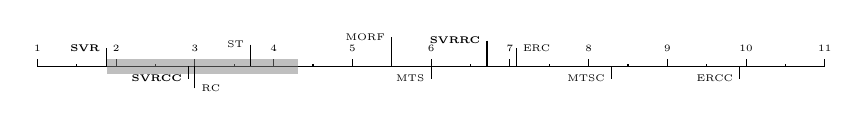
\begin{tikzpicture}
 %axis
 \draw (1,0) -- (11,0);
 \foreach \x in {1,2,3,4,5,6,7,8,9,10,11} {
  \draw (\x, 0) -- ++(0,.1) node [above,scale=0.7] {\tiny \x};
  \ifthenelse{\x < 11}{\draw (\x+.5, 0) -- ++(0,.03);}{}
 }
 % coordinates
 \coordinate (c0) at (2.92,0);
 \coordinate (c1) at (6.71,0);
 \coordinate (c2) at (1.88,0);
 \coordinate (c3) at (9.92,0);
 \coordinate (c4) at (7.08,0);
 \coordinate (c5) at (3,0);
 \coordinate (c6) at (8.29,0);
 \coordinate (c7) at (6,0);
 \coordinate (c8) at (3.71,0);
 \coordinate (c9) at (5.5,0);

 % labels
 \node (l0) at (c0) [below left=.025cm and 0cm, align=right,scale=0.7] {\tiny \textbf{SVRCC}};
 \node (l1) at (c1) [above left=.2cm and 0cm, align=right,scale=0.7] {\tiny \textbf{SVRRC}};
 \node (l2) at (c2) [above left=.1cm and 0cm, align=right,scale=0.7] {\tiny \textbf{SVR}};
 \node (l3) at (c3) [below left=.025cm and 0cm, align=left,scale=0.7] {\tiny ERCC};
 \node (l4) at (c4) [above right=.1cm and 0cm, align=right,scale=0.7] {\tiny ERC};
 \node (l5) at (c5) [below right=.15cm and 0cm, align=left,scale=0.7] {\tiny RC};
 \node (l6) at (c6) [below left=.025cm and 0cm, align=right,scale=0.7] {\tiny MTSC};
 \node (l7) at (c7) [below left=.025cm and 0cm, align=left,scale=0.7] {\tiny MTS};
 \node (l8) at (c8) [above left=.15cm and 0cm, align=right,scale=0.7] {\tiny ST};
 \node (l9) at (c9) [above left=.24cm and 0cm, align=right,scale=0.7] {\tiny MORF};

 % CD = 1.4845
 \fill[fill=gray,fill opacity=0.5] (1.88,-0.1) rectangle (4.3036,0.1);
 
 % connectors
 \foreach \x in {0,...,9} {
  \draw (l\x) -| (c\x);
 };
\end{tikzpicture}}\vspace{-1em}
\captionof{figure}{Bonferroni-Dunn test for Run Time}\label{fig:BonfDunnTime}\vspace{-1.5em}
\captionof{table}{Wilcoxon, Nemenyi, and Holm tests for Run Time}\label{tab:stattime}
\scriptsize
\resizebox{0.95\textwidth}{!}{\begin{tabular}{lccccc}
\noalign{\smallskip}\hline\noalign{\smallskip}
SVRCC vs. & Wilcoxon $R^{+}$ & Wilcoxon $R^{-}$ & Wilcoxon $p$-value & Nemenyi $p$-value & Holm $p$-value \\ 
\noalign{\smallskip}\hline\noalign{\smallskip}
SVRCC & 295.0 & 5.00 & $1.2E^{-6}$ &  $2.3E^{-1}$ & $5.0E^{-2}$\\ 
MORF & 225.0 & 75.0 & $3.2E^{-2}$ &  $3.4E^{-5}$ & $1.3E^{-2}$\\  
ST & 221.5 & 78.5 & $4.1E^{-2}$ &  $3.6E^{-2}$ & $1.7E^{-2}$\\   
MTS & 300.0 & 0.00 & $1.2E^{-7}$ &  $2.0E^{-6}$ & $1.0E^{-2}$\\ 
MTSC & 300.0 & 0.00 & $1.2E^{-7}$ &  0.0000 & $6.3E^{-3}$\\
RC & 229.0 & 71.0 & $2.3E^{-2}$ &  $2.0E^{-1}$ & $2.5E^{-2}$ \\  
ERC & 300.0 & 0.00 & $1.2E^{-7}$ & 0.0000 & $7.1E^{-3}$\\  
ERCC & 300.0 & 0.00 & $1.2E^{-7}$ & 0.0000 & $5.6E^{-3}$\\ 
SVRRC & 300.0 & 0.00 & $1.2E^{-7}$ &  0.0000 & $8.3E^{-3}$\\ 
\noalign{\smallskip}\hline\noalign{\smallskip}
\end{tabular}}
\end{table}
Table~{\ref{tab:timeresults}} shows that our proposed methods perform faster on $16$ out of the $24$ datasets. In this case, SVR performs the best on $12$ versus the $6$ of the state-of-the-art methods. The Iman-Davenport statistic $64.41$, with a $p$-value of $0.0$ which implies a statistical confidence of $100\%$. Figure~{\ref{fig:BonfDunnTime}} shows the mean rank values of each algorithm along with the critical difference value, $2.4236$, for $\alpha = 0.05$. According to the critical difference bar, there are $6$ out of $10$ algorithms beyond that perform significantly worse than our control algorithm, SVR.
According to the Wilcoxon test, shown in Table~{\ref{tab:stattime}}, SVR is shown to have significantly better performance over all algorithms with $p$-value $< 0.01$. The Nemenyi and Holm tests show that SVRCC performs significantly better than $6$ out of the $9$ algorithms and $8$ out of the $9$ algorithms with $p$-value $\leq 5.6E^{-3}$ and $p$-value $\leq 1.6E^{-2}$, respectively.

\subsection{Discussion}\label{sec:discussion}
Results indicate that our proposed methods perform competitively against the current contemporary methods, specifically SVRCC which exploits relationships among the targets. Firstly, they show that using SVR as a base-line method for multi-target chaining causes a performance improvement in model prediction, compared to other ST base-line models, as well as most MT methods. This demonstrates the advantages of using the SVR method as a base-line for multi-target learning, thus increasing the performance of the ensemble of regressor chains, SVRRC, compared to ERCC. More importantly, the results highlight the major advantage of capturing and exploiting the targets' relationships during model training. Using an ensemble of randomly generated chains does not ensure the targets' correlations are fully captured; however, using a maximum correlation chain improves the performance in terms of quality metrics as well as run time. The run time of SVR was shown to be the fastest, due to the fact that its complexity is mostly dependent on the number of targets. However, this method does not consider any of the correlations that might exist among the target variables, but SVRCC does take them into account and does not have a significant impact on run time. The most noteworthy finding that highlights advantage of using the base-line SVR and the maximum correlation method, SVRCC, rather than random chaining as done in ERCC, are the run time results and their analysis. ERCC had the worst run time across all datasets, whereas our proposals, SVR and SVRCC, performed the fastest. This emphasizes the advantage of using a single chain rather an ensemble of random chains, especially when the single chain is ordered in the direction of the targets maximum correlation.

\section{Conclusions}\label{sec:MTRconclusions}
This contribution proposed three novel methods for solving multi-target regression problems. The first method takes a \textit{problem transformation} approach, which generates $m$ ST models, each trained independently. This base-line approach was shown to perform the best in terms of run time, but its drawback  is that it does not take the possible correlations between the target variables into account during training. The second implements SVR as an ensemble model of randomly generated chains, inspired by the classification method ERCC. This was done to investigate the effects of exploiting correlations among the target variables during model training. Due to the random nature of this method, capturing target correlations is not guaranteed. The third proposal, SVRCC, generates a single chain that is ordered in the direction of the targets' maximum correlation, ensuring the correlations among targets are taken into account within the learning process.

The experimental study compared the proposed methods' performances to $7$ popular, contemporary methods on 24 MT regression datasets. Firstly, the results show the superior performance of using the SVR method as a base-line model, rather than regression trees as used in MORF. The results for SVRRC show an increase in performance when random chaining is used to develop an ensemble model. This indicates the importance of the relationship among the target variables during training. Finally, the results show the superiority of using the SVRCC method, which was ranked the best in all quality metrics and second best in terms of run time. SVRCC performed better than the single-target SVR model and the randomly chained ensemble model SVRRC, showing that the targets' maximum correlation does positively contribute toward model training. The statistical analysis supports and shows the significance of the results obtained by our experiments. They demonstrated that statistically significant differences exist between the proposed algorithms against the methods compared. SVRCCs competitive performance, as well as speed, shows that it is a powerful learning algorithm for multi-target problems. The research outcomes of this chapter have been published in~\cite{melki2017multi}.

\chapter{Multi-Instance SVM using Bag-Representatives \label{chap:mirsvm}}
This contribution of this chapter proposes a novel support vector machine (SVM) formulation under the multiple-instance learning (MIL) paradigm. It also presents a novel algorithm and  bag representative selector that trains the SVM using bag-level information, named Multi-Instance Representative SVM (MIRSVM). The contribution is able to identify instances that highly impact classification, i.e. the \textit{bag-representatives}, for both positive and negative bags, while finding the optimal class separation hyperplane. Unlike other multi-instance SVM methods, this approach eliminates possible class imbalance issues by allowing both positive and negative bags to have at most one representative, which constitute as the most contributing instances to the model. The experimental study evaluates and compares the performance of this proposal against $11$ popular and widely used multi-instance methods over $15$ datasets, and the results are validated through non-parametric statistical analysis. The results indicate that bag-based learners outperform the instance-based and wrapper methods, and emphasize this proposal's overall superior performance against other multi-instance SVM models. 

\section{Multi-Instance Classification Background}\label{sec:mibackground}
This section defines the notation that will be used throughout this chapter and reviews related works pertaining to multiple-instance learning, specifically the concepts of instance-based and bag-based learners are discussed and compared, along with algorithms within those paradigms.

\subsection{Notation}\label{subsec:minotation}
Let $\mathcal{D}$ be a training dataset of $n$ bags. Let $\bm{Y} \in \mathcal{D}$ be a vector of $n$ labels corresponding to each bag, having a domain of $\bm{Y} \in \set{-1,1}^n$. Let $\bm{X} \in \mathcal{D}$ be a matrix consisting of $d$ input variables and $m$ instances, $\bm x_i \in \bm X,\, \forall i \in \set{1,\ldots,m}$ , having a domain of $\bm{X} \in \mathbb{R}^{m \times d}$. Let $\mathcal{B}$ be the set of bags which contain $|\mathcal{B}_I|$ number of instances, sometimes of different size and usually non-overlapping, such that $\mathcal{B}_I = \{\bm x_{1}, \ldots, \bm x_{|\mathcal{B}_I|}\}$ for index set $I \in \set{1,\ldots,n}$. 

\begin{table}[t!]
\small
\caption{Summary of Multiple-Instance Learning Notation}\label{tab:MILNotation}
\begin{tabularx}{\textwidth}{l@{\extracolsep{\fill}}l}
\hline\noalign{\smallskip}
Definition & Notation\\ 
\noalign{\smallskip}\hline\noalign{\smallskip}
Number of Bags & $n$ \\
Number of Instances & $m$ \\
Number of Input Attributes & $d$ \\
Set of Bags & $\mathcal{B} = \set{\mathcal{B}_1,\, \ldots,\, \mathcal{B}_n}$ \\
Bag Index Set & $I \in \ints_+^n$ \\
Input Space & $\bm{X} \in \mathbb{R}^{m \times d}$ \\
Bag Labels & $\bm{Y} \in \{-1,1\}^n$ \\
Input Instance $i$ from Bag $I$ & $\bm{x}_i \in \bm{x}_i = (x_{i1}, \ldots, x_{id}),\, \forall i \in \set{1,\ldots,n},\, i \in I$ \\
Unknown Individual Instance Label $i$ & $y_i \in \set{-1,1}$ \\
Bag $I$ & $\mathcal{B}_I = \set{\bm x_i \st \forall i \in I}$ \\
\noalign{\smallskip}\hline\noalign{\smallskip}
Full Multi-Instance Training Dataset & $\mathcal{D} = \{(\mathcal{B}_1,Y_1), \ldots, (\mathcal{B}_n,Y_n)\}$ \\
\noalign{\smallskip}\hline
\end{tabularx}
\end{table}

\subsection{Multi-Instance Classification Methods}
The difference between MIL and traditional learning lies in the nature of the data. In the traditional binary classification setting, the goal is to learn a model that maps input samples to labels, $f: \reals^{m \times d} \rightarrow Y^m \in \set{-1,\,+1}$. In the multi-instance setting, samples are called \textit{bags} and each bag contains one or more input instances and is assigned a single bag-level label. Input instances, $\set{\bm x_1,\, \bm x_2,\, \ldots,\, \bm x_m}$, are grouped into bags with unique identifiers, $\mathcal{B} = \set{\mathcal{B}_1,\, \mathcal{B}_2,\, \ldots,\, \mathcal{B}_n \st \mathcal{B}_I = \set{\bm x_i \st \forall i \in I},\, \forall I \in \set{1, \ldots, n}}$ and assigned a label, $Y_I$. The individual instance labels within a bag are unknown. Traditionally, MIL has focused on binary classification problems, however, there are cases where the number of classes can be larger, i.e. $\bm Y \in \ints^n$. The scope of this chapter will consist of binary multiple instance classification problems. 

Using the training dataset $\mathcal{D} = \{(\mathcal{B}_1,Y_1), \ldots, (\mathcal{B}_n,Y_n)\}$, the goal is to train a classifier that predicts the label of an unseen bag, $f(\mathcal{B}_{n+1}) \rightarrow Y_{n+1}$~\cite{Amores2013}. In order to build a classifier without any knowledge of the individual training instance labels, Dietterich et. al.~\cite{Dietterich1997} proposed the \textit{standard MI} (SMI) hypothesis, shown in Equation~\eqref{eqn:stas}, which states that a bag is labeled positive if and only if at least one of the instances in the bag is positive, and is labeled negative otherwise.
\begin{equation}
\centering \label{eqn:stas}
 Y_I = \begin{cases}
			+1 & \text{if }\exists\, y_i = +1,\, \forall i \in I \\
			-1 & \text{otherwise}.
		  \end{cases}
\end{equation}

This implies that individual instance labels $y_i$ exist, but are not known (for positive bags) during training. Equation~\eqref{eqn:stas} can also be rewritten as Equation~\eqref{eqn:stasmax} for simplicity:
\begin{equation}
\centering \label{eqn:stasmax}
Y_I = \text{argmax}_{\forall i \in I}\,\,\, y_i.
\end{equation}

In addition to the SMI assumption, alternative MI assumptions have been proposed to date~\cite{Foulds2010}. A recent review~\cite{Amores2013} describing the taxonomy of multi-instance classification presents various methods and algorithms used in literature, which are categorized based on their approach to handling the MI input space. Instance-based classifiers that fall under the \textit{instance-space paradigm}, aim to separate instances in positive bags from those in negative ones. Bag-level classifiers (\textit{bag-space paradigm}) treat each bag as a whole entity, implicitly extracting information from each bag in order to accurately predict their labels. Methods that fall under the \textit{embedded-space paradigm} map the input bags to a single feature vector that explicitly encapsulates all the relevant information contained within each bag.

Instance-based methods that follow the SMI assumption attempt to identify desirable instance properties that make a bag positive. A simple and natural way of addressing this type of learning problem is to assume that each instance in a bag has the same label as the bag itself. After that, a single-instance classifier can be trained on the transformed dataset, and finally, the SMI assumption can be applied over the predicted instance labels of unseen bags~\cite{Ventura2016}. Methods that employ this type of approach are called \textit{Wrapper} methods; they act as an interface between the instance and bag levels. One algorithm that employs this approach is called Simple-MI~\cite{Dong2006}. Simple-MI represents each bag with the mean vector of the instances within it. Another example is MIWrapper~\cite{Frank2003}, which introduces weights to treat instances from different bags differently. The major disadvantage of wrapper techniques is that they assume the distribution the instances in positive bags is positive, when it may not be, thus imposing noise over the positive class.

One traditional instance-based method that takes a different approach is the Axis-Parallel Rectangle (APR)~\cite{Dietterich1997}, which trains a model that assigns a positive label to an instance if it belongs to an axis-parallel rectangle in feature space, and assigns a negative label otherwise. The APR method is optimized by maximizing the number of positive bags in the training set containing at least one instance in the APR, while concurrently maximizing the number of negative bags that do not contain any instance in the APR. 

Another similar and popular approach that falls under maximum likelihood-based methods, is the Diverse Density (DD)~\cite{Maron1998} framework. The DD metric is maximized for instances in feature space that are near at least one instance in a positive bag and far from all instances in negative bags. In the Expectation-Maximization Diverse Density (EM-DD) algorithm, Zhang and Goldman~\cite{Zhang2001} propose a similar framework that iteratively maximizes the DD measure. Auer and Ortner~\cite{Auer2004} present a boosting approach that uses balls centered around positive bags to solve the MI problem called Multi-Instance Optimal Ball (MIOptimalBall). This approach is similar to that of APR and DD, except that Auer and Ortner~\cite{Auer2004} propose computing optimal balls per positive bags. A major challenge affecting these methods is that the distributions of the positive and negative bags affect their performance. Methods based on the DD metric~\cite{Carbonneau2016,Chen2006,Chen2004} assume the positive instances form a cluster, which may not be the case. Alternatively, Fu et al.\cite{Fu2011} models the distribution of negative bags with Gaussian kernels, which can prove difficult when the quantity of data is limited.

As mentioned previously in brief, the classical method of boosting~\cite{freund1996experiments,schapire1999improved} has been adapted to a multi-instance instance-based algorithm. For example, Viola et al.~\cite{zhang2006multiple} proposed an adaptation of boosting to the multi-instance paradigm based on the standard MI assumption, named MILBoost. Later, inspired by the MILBoost~\cite{zhang2006multiple} and Online-ADABoost~\cite{oza2001online} algorithms, Babenko et al.~\cite{babenko2009visual} developed a novel online MI boosting method which lead to a robust and stable model in the area of object tracking. All the works mentioned, including many other such as~cite{qi2011online,xie2012online}, have positively contributed and inspired many approaches in the area of visual detection and tracking.

An extension of traditional single-instance $k$-nearest neighbors method ($k$-NN) was proposed by Wang and Zucker~\cite{Wang2000} to be applied to the bag-level, named CitationKNN. This method uses a distance function between bags in order to determine bag similarities. Not only are the set of closest bags to a single bag  considered, but also how many bags is the single bag closest to. A voting scheme is then used to determine the bag class labels.

Blockeel et al.~\cite{Blockeel2005} introduced the Multi-Instance Tree Inducer (MITI), based on the standard MI assumption, which uses decision trees as a heuristic to solve the MI problem. This approach aims to identify whether an instance within a bag is truly positive and eliminate false positives within the same bag. The disadvantage of this approach stems from removing instances considered as false positives from partially grown trees without updating the existing tree structure. Bjerring and Frank~\cite{Bjerring2011} then enhanced this approach by creating the method Multi-Instance Rule Induction (MIRI). The algorithm aims to eliminate any possibility of a suboptimal split because the tree is discarded and regrown. 

The MI adaptation of the SVM presents two contexts for solving the problem: the instance-level and the bag-level. The first tries to identify instances, either all within a bag or just key instances, that help find the optimal separating hyperplane between positive and negative bags. The latter uses kernels defined over whole bags to optimize the margin~\cite{Doran201479}. 

Andrews et. al.~\cite{Andrews2002} proposed a mixed-integer quadratic program that solves the MI problem at an instance-level, using a support vector machine, named MISVM, that can be solved heuristically. Rather than maximizing the margin of separability between instances of different classes, this instance-based method maximizes the margin between bags. It tries to identify the key instance from each positive bag that makes the bag positive by assuming it has the highest margin value. Instances from positive bags are selected as bag-representatives, and the algorithm iteratively creates a classifier that separates those representatives from all instances from the negative bags. Using bag-representatives from one class and all instances from the other is an example of an approach that combines rules from the SMI assumption and the collective assumption. A disadvantage of this approach stems from the assumption that all instances within positive bags are also positive, which is an implicit step in the initialization of MISVM. Andrews et. al.~\cite{Andrews2002} also proposed a second mixed-integer instance-level approach, named mi-SVM, which does not discard the negative instances of the positive bags. It rather tries to identify the instances within positive bags that are negative and utilize them in the construction of the negative margin. The main disadvantage of these approaches is that they create an imbalanced class problem that favors the negative class, resulting in a biased classifier.

Asymmetric SVM (ASVM), presented by Yang et al.~\cite{Herman2008}, was designed to use an asymmetric loss function under the SMI assumption. This approach was based on the idea that the cost of misclassification is different for positive and negative bags. For example, a false negative instance in a positive bag would not necessarily introduce an error on the bag label, assuming there are many positive instances within the bag. However, a false positive instance in a negative bag would definitely lead to an error. Using rules such as these, ASVM aims to minimize false positives, while ensuring all negative instances are on the negative side of the hyperplane.

The approach presented by Cheung et al.~\cite{cheung2006regularization} presented a loss function that takes the cost associated with bag labels and the cost (under the SMI assumption) between prediction of beach bag and its instances into account. They also presented an SVM regularization scheme as well which, rather than using a heuristic method, used concave-convex optimization, ensuring local-optimum convergence.

An example of using the approach of a bag-level kernel would coincidentally be one of the first bag-level approaches to the multi-instance SVM problem, proposed by G{\"a}rtner et. al.~\cite{Smola2002}. A bag-level kernel determines the similarity between two bags in a higher dimensional space. Blaschko et. al.~\cite{Blaschko2006} proposed conformal kernels which manipulate each attribute's dimension based on its importance, without affecting the angles between vectors in the transformed space. These type of bag level kernels transform the bags into a single-instance representation which enables standard SVMs to be directly applied to multi-instance data. 

Unlike the bag-based methods mentioned previously, which have a the SMI assumption embedded in their design, mapping-based algorithms do not assume a specific relationship exists between the labels of each bag and its instances. Rather, the relationship is learned from the data. An example of such methods is the Two-Level Classifier (TLC)~\cite{Weidmann2003}. Another example, which includes the use of kernels in the multi-instance bag-space setting, would be approach taken by Zhou et al.~\cite{zhou2009multi}. The basic idea behind their method is to treat instances in an non-i.i.d. manner, thus exploiting relationships among instances using a graph kernel. 

Wang and Zucker~\cite{wang2000solving} proposed CitationKNN which extends the traditional $k$-nearest neighbors ($k$-NN) method to the bag-level. To classify a new bag $\mathcal{B}$, CitationKNN uses a distance function that operates at the bag level to determine which bags are the closest to $\mathcal{B}$. It not only considers the bags that are closest, but also the bags for which $\mathcal{B}$ is in the set of closest bags to others. Any bag-based distance function can be used by CitationKNN.

For most of the methods described above, implicit or explicit assumptions have been made about the distribution of the data. Selecting a method that is robust for a problem such as MIL can be difficult when little is known about the nature of the data, especially considering the unknown distribution of the instances within bags~\cite{Amores2013}. The proposed method, MIRSVM, is a general method that uses support vector machines to design a MIL model without making prior assumptions about the data. Classifiers of this type are known to provide better generalization capabilities and performance, as well as sparser models.

\section{MIRSVM: A Novel SVM for Multi-Instance Classification}
MIRSVM is based on the idea of selecting representative instances from both positive and negative bags which are used to find an unbiased, optimal separating hyperplane. A representative is iteratively chosen from each bag, and a new hyperplane is formed according to the representatives until they converge. Based on the SMI hypothesis, only one instance in a bag is required to be positive for the bag to adopt a positive label. Due to the unknown distribution of instances within positive bags, MIRSVM is designed to give preference to negative bags during training, because their distribution is known, i.e. all instances are guaranteed to be negative. This is evident during the representative selection process, by taking the index of the maximum output value within each bag based on the current hyperplane using the following rule, $s_I = \text{argmax}_{i \in I} (\langle \bm w,\, \bm x_i \rangle + b),\, \forall I \in \set{1,\ldots,n}$. In other words, the most positive instance is chosen from each positive bag and the least negative instance is chosen from each negative bag (instances with the largest output value based on the current hyperplane), pushing the decision boundary  towards the positive bags. 

Equation~\eqref{eq:primalmirsvm} presents the primal MIRSVM optimization problem:
\begin{subequations} 
\label{eq:primalmirsvm}
\begin{alignat}{2}
\min\limits_{\bm w, b,\bm\xi}& {\,\,} \frac{1}{2}||\bm{w}||^2 + C\sum_I \xi_I, \tag{\ref{eq:primalmirsvm}}\\ 
\text{s.t.}& {\,\,} Y_I(\langle\bm{w},\bm x_{s_I}\rangle + b) \geq 1 - \xi_I,\, \forall I \in \set{1,\ldots,n}  \label{eq:primalmirsvm1}\\
{} & {\,\,} \xi_I \geq 0,\, \forall I \in \set{1,\ldots,n}, 
\end{alignat}
\end{subequations} 
where $\bm S_I$ is the set of the bag representatives' indices and $\bm x_{s_I}$ is the instance representative of bag $\mathcal{B}_I$. Note the variables in MIRSVMs formulation are the similar to those of the traditional SVM, except they are now representing each bag as an instance. Solving the optimization problem given in Equation~\eqref{eq:primalmirsvm} using a quadratic programming solver is a computationally expensive task due to the number of constraints, which scales by the number of bags $n$, as well as the calculation of the inner product between two $d$-dimensional vectors in constraint~\eqref{eq:primalmirsvm1}. The proposed solution for these problems was deriving and solving the dual of the optimization problem given by Equation~\eqref{eq:primalmirsvm}. 

The dual can be formed by taking the Lagrangian of~\eqref{eq:primalmirsvm}, given by Equation~\eqref{eqn:svmlagrangian}, where $\bm \alpha$ and $\bm \beta$ are the non-negative Lagrange multipliers.
\begin{equation}
\centering \label{eqn:svmlagrangian}
\resizebox{.9\textwidth}{!}{$
\begin{aligned}
\mathcal{L}\left(\bm{w},b,\bm{\xi},\bm{\alpha},\bm{\beta}\right) = \frac{1}{2}\sum_{j=1}^d w_j^2  + C\sum_I \xi_I - \sum_I{\beta_I \xi_I} - \sum_I{\alpha_I\left(Y_I\left(\sum_{j=1}^d w_j x_{s_Ij} + b\right) -1 + \xi_I\right)}
\end{aligned}$} 
\end{equation}

At optimality~\cite{Boyd2004}, $\bigtriangledown_{w,b,\xi}\mathcal{L}(\bm{w},b,\bm{\xi},\bm{\alpha},\bm{\beta}) = 0$ and the following conditions are met:
\begin{align}
&\frac{\partial\mathcal{L}}{\partial w_j}: w_j = \sum_I{\alpha_I\,Y_I\, x_{s_I\,j}},\,\forall j \in \{1,\ldots,d\}\label{eqn:optcond1}\\
&\frac{\partial\mathcal{L}}{\partial b}: \sum_I{\alpha_IY_I} = 0,\label{eqn:optcond2}\\
&\frac{\partial\mathcal{L}}{\partial\xi_I}: \alpha_I + \beta_I = C,\,\forall I \in \set{1,\ldots,n}\label{eqn:optcond3} 
\end{align}

By substituting Equations~\eqref{eqn:optcond1},~\eqref{eqn:optcond2}, and~\eqref{eqn:optcond3} into the Lagrangian in~\eqref{eqn:svmlagrangian}, the dual MIRSVM formulation becomes the following:
\begin{subequations} 
\label{eq:dualmirsvm1}
\begin{alignat}{2}
\max\limits_{\bm \alpha,\bm \beta}& \sum_I \alpha_I -\frac{1}{2}\sum_I \sum_{K\in I} \sum_{j=1}^d \alpha_I \alpha_K Y_I Y_K  x_{s_I j} x_{s_K j} \tag{\ref{eq:dualmirsvm1}}\\
\text{s.t.}&  \sum_I{\alpha_IY_I} = 0\, \\
{} & \alpha_I + \beta_I = C,\,\forall I \in \set{1,\ldots,n}   \label{eq:implicit1}\\
{} & \alpha_I \geq 0,\, \forall I \in \set{1,\ldots,n}  \label{eq:implicit2} \\
{} & \beta_I \geq 0,\, \forall I \in \set{1,\ldots,n},  \label{eq:implicit3}
\end{alignat}
\end{subequations} 
where $s_I$ is computed for each bag, as shown in Equation~\eqref{eq:si}:
\begin{equation}
\label{eq:si}
\centering
s_I = \underset{i \in I}{\text{argmax}}(\sum_{K\in I} \sum_{j=1}^d \alpha_K Y_K x_{s_K j} x_{ij} + b),\, \forall I \in \set{1,\ldots,n}.
\end{equation}

The implicit constraints~\eqref{eq:implicit1} through~\eqref{eq:implicit3} imply three possible cases for $\alpha_I$ values:
\begin{itemize}
\item[1.] If $\alpha_I = 0$, then $\beta_I = 0$ and $\xi_I = 0$, implying the instance is correctly classified and outside the margin. 
\item[2.] If $0 < \alpha_I < C$, then $\xi_I  = 0$, and the instance is a support vector and site on the margin boundary, i.e. is an \textit{bounded support vector}.
\item[3.] If $\alpha_I = C$, then there is no restriction for $\xi_I > 0$. This also indicates that the instance is a support vector, but one that is \textit{unbounded}. If $0 < \xi_I < 1$, then the instance is correctly classified, and is misclassified if $\xi \geq 1$. 
\end{itemize}

The dual is then kernelized by replacing the inner product of samples in feature space with their corresponding kernel value, $\spa{K}\left(\bm{x}_{s_I},\bm{x}_{s_K}\right)$. The dual function is now written as:
\begin{subequations} 
\label{eq:dualmirsvm}
\begin{alignat}{2}
\max\limits_{\bm \alpha}& \sum_I \alpha_I - \frac{1}{2}\sum_I \sum_{K\in I} \alpha_I \alpha_K Y_I Y_K  \spa{K}\left(\bm{x}_{s_I},\bm{x}_{s_K}\right) \tag{\ref{eq:dualmirsvm}}\\
\text{s.t.}&  \sum_I{\alpha_IY_I} = 0\,  \\
{} & 0 \leq \alpha_I \leq C,\, \forall I \in \set{1,\ldots,n}.
\end{alignat}
\end{subequations} 

One of the biggest advantages of the dual SVM formulation is the sparseness of the resulting model. This is because support vectors, instances that have their corresponding $\alpha_I \neq 0$, are only considered when forming the decision boundary. MIRSVM uses a Gaussian RBF kernel, given by Equation~\eqref{eq:gaussiankernel}, where $\sigma$ is the Gaussian shape parameter.
\begin{equation}
\label{eq:gaussiankernel}
\centering
\mathcal{K}(\bm x_i, \bm x_j) = e^{-\frac{\norm{\bm x_i - \bm x_j}^2}{2\sigma^2}}
\end{equation}

To evaluate the output vector, $\bm o_I$, of bag $I$ using the kernel, the following equation is used, where $\mathcal{B}_I$ are the instances of bag $I$, $\bm X_S$ are the optimal bag representatives, and $\bm Y_S$ are the representative bag labels.
\begin{align}
\bm o_I = \spa{K}(\mathcal{B}_I,\bm X_S)*(\bm\alpha \cdot \bm Y_S) + b
\end{align}

\newpage

The bias term $b$ is calculated as shown in Equation~\eqref{eqn:bias}, where $\bm{sv}$ is the vector of support vector indices and $n_{sv}$ is the number of support vectors~\cite{Huang2006}.
\begin{align}
\label{eqn:bias}
b = \frac{1}{n_{\bm{sv}}}\sum_{\bm{sv}} Y_{\bm{sv}} - \spa{K}(\bm X_{\bm{sv}},\bm X_{\bm{sv}})*(\bm \alpha_{\bm{sv}}\bm\cdot Y_{\bm{sv}})
\end{align}

\begin{figure}[t!]
\centering
\small
\label{fig:mirsvm}
\begin{minipage}{\textwidth}
\small
\adjustbox{scale=0.9}{
\begin{tikzpicture}[%
    node distance=4cm,
    on grid,
    auto
  ]
\node[block](A) {Initialize $\bm S$ randomly};
\node(B)[block, right of=A, text width=6em] {Train SVM using QP solver over $\bm S$, set $\bm S_{old} = \bm S$};
\draw[arrow] (A) -- (B);
\node(C)[block, right of=B,text width=6.3em] {Find optimal representatives, $\bm S$, for the current hyperplane};
\draw[arrow] (B) -- (C);
\node(D) [decision,right of=C,fill=gray!55,text width=2cm]{while $\bm S$ has not changed, $\bm S \neq \bm S_{old}$};
\draw[arrow] (C) -- (D);
\node(E) [block,right of=D]{return $\bm \alpha,\, b, \bm S$};
\draw[arrow] (D) -- node {yes} (E);
\draw[arrow] (D.north) --+(0,0.1cm) -| (B.north) node[below,pos=0.25] {no} ;
\end{tikzpicture}}
\caption{\small A summary of the steps performed by MIRSVM. The representatives are first randomly initialized and continuously updated according to the current hyperplane. Upon completion, the model is returned along with the optimal bag-representatives.}
\end{minipage}
\begin{minipage}{\textwidth}
\begin{algorithm}[H]
\small
\caption{Multi-Instance Representative SVM (MIRSVM)}
\label{alg:mirsvm} 
\begin{algorithmic}
\renewcommand{\algorithmicrequire}{\textbf{Input:}}
\renewcommand{\algorithmicensure}{\textbf{Output:}}
\Require Training dataset $\mathcal{D}$, SVM Parameters $C$ and $\sigma$
\Ensure  SVM model parameters $\bm \alpha$ and $b$, Bag Representative IDs $\bm S$
\For {$I \in \set{1,\ldots,n}$}
\State $\bm S_I \leftarrow \text{ rand}\left(|\mathcal{B}_I|,1,1\right)$ \Comment{Assign each bag a random instance}
\EndFor
\While {$\bm S \neq \bm S_{old}$}
\State $\bm S_{old} \leftarrow \bm S$
\State $\bm X_S \leftarrow \bm X(\bm S),\,\bm Y_S \leftarrow \bm Y(\bm S)$ \Comment{Initialize the representative dataset}
\State $\bm G \leftarrow (\bm Y_S \times \bm Y_S) \bm \cdot \mathcal{K}\left( \bm X_S,\,\bm X_S,\,\sigma\right)$ \Comment{Build Gram matrix}
\State $\bm \alpha \leftarrow \text{ quadprog}\left(\bm G, \bm{-1}^n, \bm Y_S, \bm 0^n, \bm 0^n, \bm C^n\right)$ \Comment{Solve QP Problem}
\State $\bm{sv} \leftarrow \text{find}\left(0 < \bm \alpha \leq C \right)$ \Comment{Get the support vector indices}
\State $n_{\bm{sv}} \leftarrow \text{count}\left(0 < \bm \alpha \leq C \right)$ \Comment{Get the number of support vectors}
\State $b \leftarrow \frac{1}{n_{\bm{sv}}}\sum_{i=1}^{n_{\bm{sv}}} \left(\bm Y_{\bm{sv}} - \bm G_{\bm{sv}}*\left(\bm{\alpha_{\bm{sv}}} \cdot \bm Y_{\bm{sv}}\right)\right)$ \Comment{Calculate the bias term}
\For {$I \in \set{1,\ldots,n}$} 
\State $\bm G_I \leftarrow (Y_I \times \bm Y_S) \bm \cdot \mathcal{K}\left( \mathcal{B}_I,\,\bm X_S,\,\sigma\right)$
\State $\bm S_I \leftarrow \text{argmax}_{i \in I}\left(\bm G_I*\bm{\alpha} + b \right)$ \tab\tab[0.62cm]\Comment{Select optimal bag-representatives}
\EndFor
\EndWhile 
\end{algorithmic}
\end{algorithm}
\end{minipage}
\end{figure}

Algorithm~\ref{alg:mirsvm} shows the procedure for training the multi-instance representative SVM classifier and obtaining the optimal representatives from each bag.  During training, the representatives, $\bm S$, are first initialized by randomly selecting an instance from each bag. A hyperplane is then obtained using the representative instances, and new optimal representatives are found with respect to the current hyperplane, by using the rule given in Equation~\eqref{eq:si}. At each step, the previous values in $\bm S$ are stored in $\bm S_{old}$. The training procedure ends when the bag representatives stop changing from one iteration to the next ($\bm S = \bm S_{old}$). Examples of the convergence of bag-representatives are shown in Figure~\ref{fig:convegence}. During the testing procedure, each bag produces an output vector based on the hyperplane found in the training procedure. The bag label is then assigned by taking the sign of the output vector's maximum value, following the SMI assumption. 

\begin{figure}[t!]
\centering
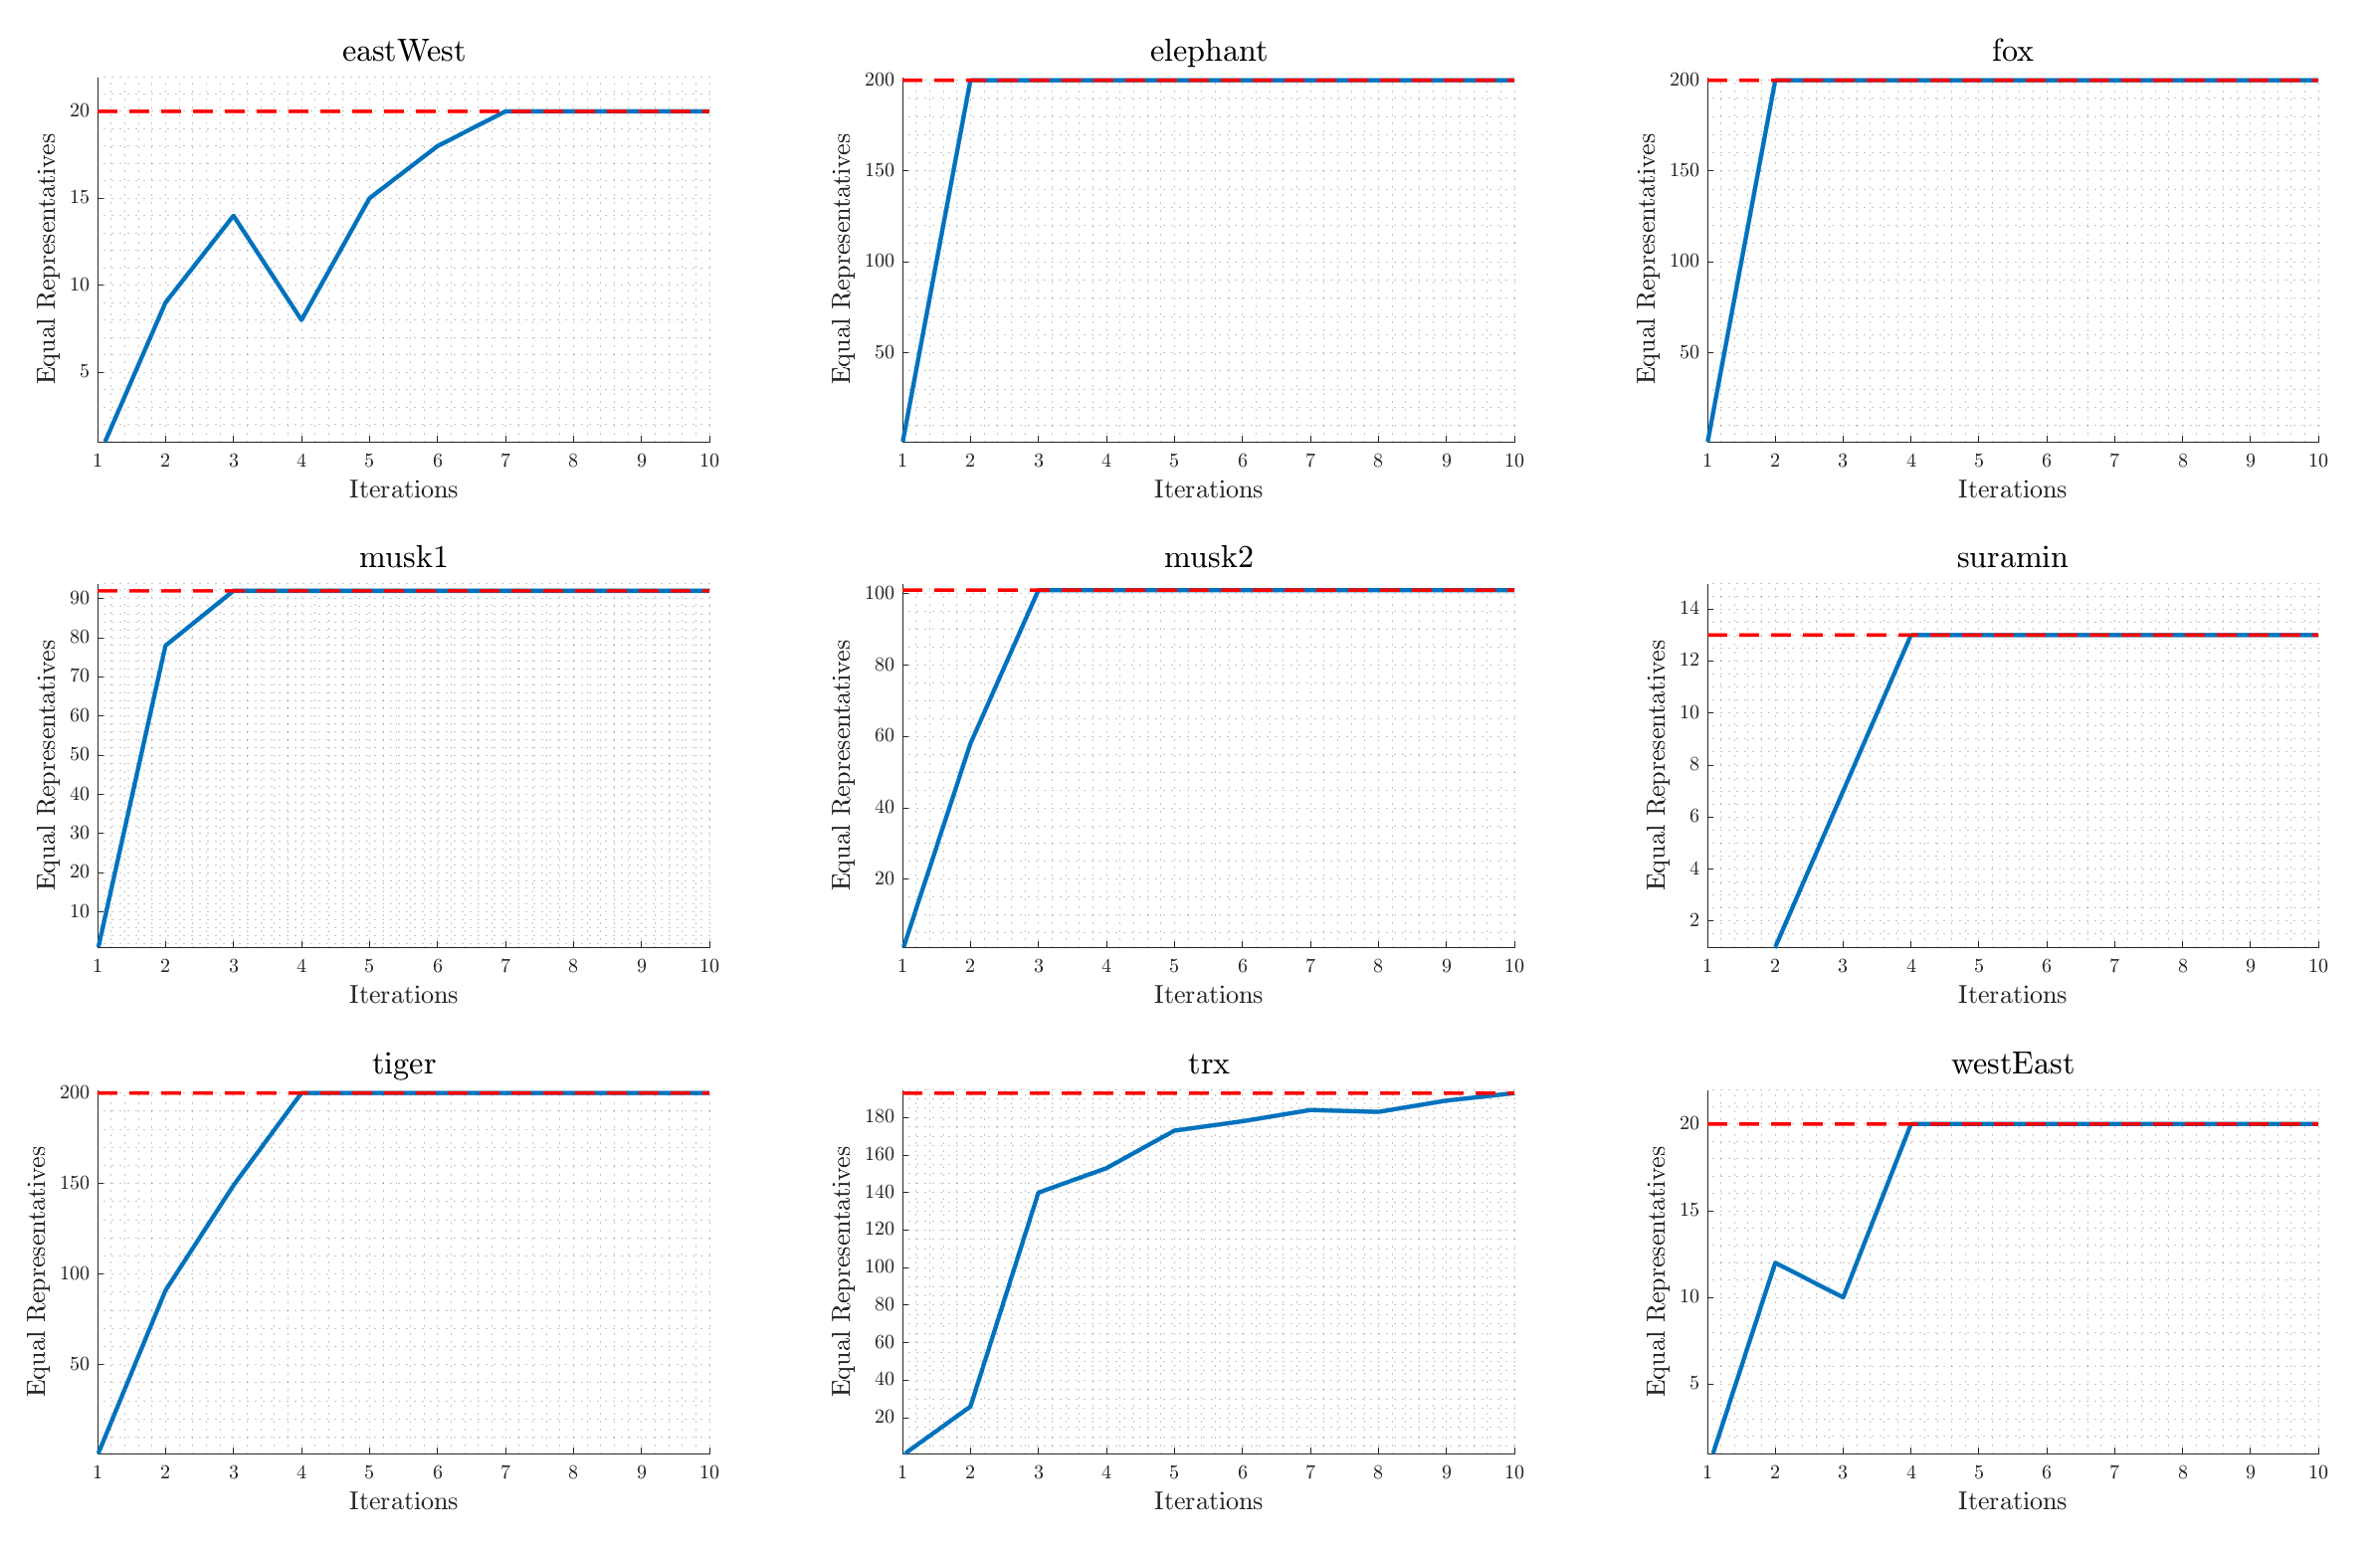
\includegraphics[width=0.94\textwidth]{figures/convergence.png} 
\caption{Bag representative convergence plots on 9 datasets. The blue line shows the number of bag representatives that are equal from one iteration to the next. The red dashed line represents the total number of bags.}\label{fig:convegence}
\end{figure}

\begin{figure}[t!]
    \centering
    \begin{minipage}{0.5\textwidth}
        \centering
        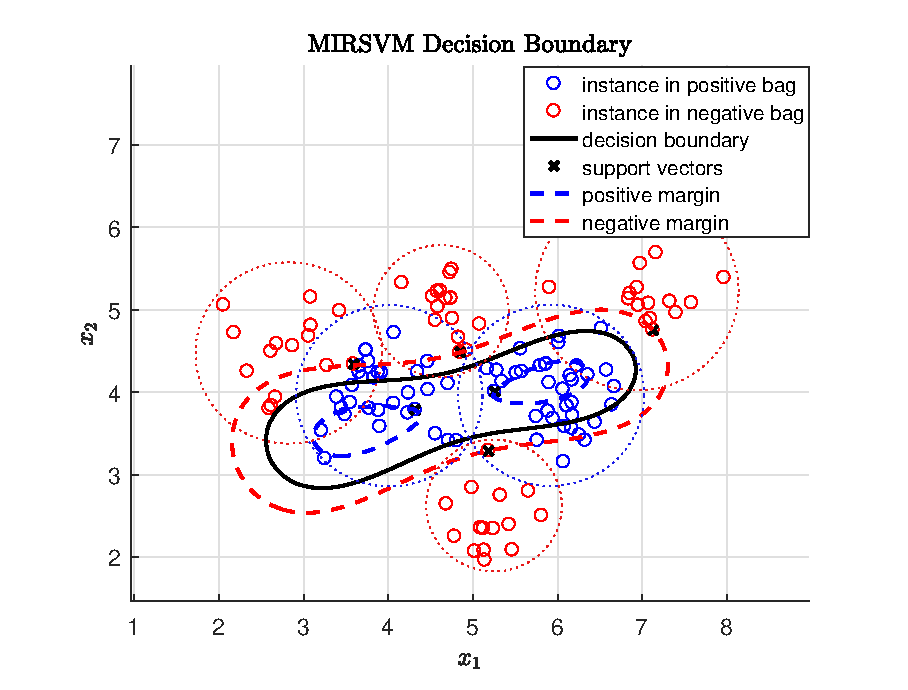
\includegraphics[width=\textwidth]{figures/mirsvm_figure.eps} % first figure itself
    \end{minipage}\hfill
    \begin{minipage}{0.5\textwidth}
        \centering
        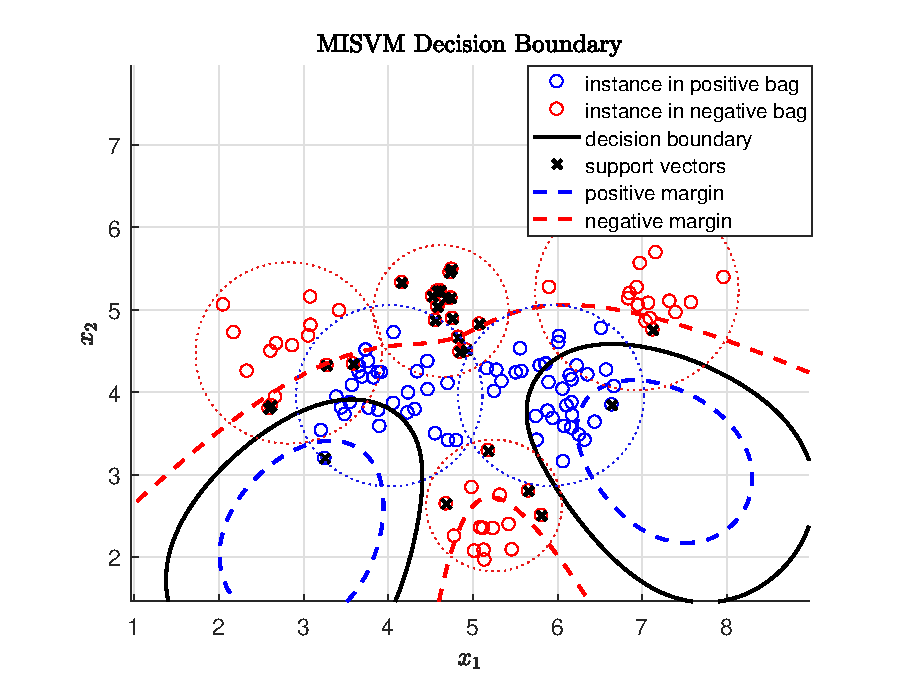
\includegraphics[width=\textwidth]{figures/misvm_figure.eps} % second figure itself
    \end{minipage}
    \caption{Difference between MIRSVM and MISVM on a random $2$-dimensional toy dataset. Note the differing number of support vectors produced by the two methods. MIRSVM has $6$, one for each bag, and MISVM has $29$. Also note the smoother representation of the data distribution given by MIRSVM's decision boundary, unlike MISVM whose decision boundary was greatly influenced by the larger number of support vectors belonging to the negative class with respect to the only $2$ positive support vectors.}\label{fig:diff}
\end{figure}

This formulation is designed to utilize and select representatives from positive and negative bags, unlike MISVM, which only optimizes over representatives from positive bags, while flattening the negative bag instances. MISVM allows multiple representatives to be chosen from negative bags and limits positive bag-representatives to be one, while MIRSVM allows for balanced bag-representative selection, where each bag is allowed one. MISVM also uses a wrapper method to initialize the positive bag-representatives by taking the mean vector of the instances within each positive bag. This is an implicit assumption that the instances within the positive bags are all positive, whereas MIRSVM's initialization procedure selects an instance from all bags at random, ensuring no noise is added by any wrapper techniques during initialization and no assumptions are made about the instances. Due to the constraints on the representatives, MIRSVM produces sparser models while MISVM has the freedom to select as many negative support vectors as it needs and restricts the support vectors chosen from positive bags to be one. Figure~\ref{fig:diff} shows the decision boundaries produced by MIRSVM and MISVM to highlight the differences in their solutions. As Figure~\ref{fig:diff} shows, MISVM produces a larger number of support vectors from the negative bags, which greatly influences the final decision boundary in favor of the negative class.

\section{Experimental Environment}
This section presents the experimental setup and comparison of our contribution, as well as $11$ other widely used methods on $15$ different benchmark datasets. The main aim of the experiments is to compare our contribution to other multi-instance support vector machines, contemporary multi-instance learners, and ensemble methods. 

Table~\ref{tab:Dataset} presents a summary of the $15$ datasets used throughout the experiments, where the number of attributes, bags, and total number of instances are shown. The datasets were obtained from the Weka\footnote{http://www.cs.waikato.ac.nz/ml/weka}~\cite{Hall2009} and KEEL\footnote{http://sci2s.ugr.es/keel/datasets.php}~\cite{Alca2011} dataset repositories. 

\begin{table}[t!]
\centering
\caption{Multi-Instance (MI) Classification datasets}
\small
\label{tab:Dataset}
\resizebox{\textwidth}{!}{\begin{tabularx}{1.1\textwidth}{l@{\extracolsep{\fill}}rrrrrr}
\hline\noalign{\smallskip}
Dataset & Attributes & Positive Bags & Negative Bags & Total & Instances & Avg. Bag Size\\
\noalign{\smallskip}\hline\noalign{\smallskip}
Suramin & 20 & 7 & 6 & 13 & 2898 &  222.92 \\ 
EastWest & 24 & 10 & 10 & 20 & 213 &  10.65  \\ 
WestEast & 24 & 10 & 10 & 20 & 213 &  10.65  \\ 
Musk1 & 166 & 47 & 45 & 92 & 476 &  5.17  \\ 
Musk2 & 166 & 39 & 62 & 101 & 6728 &  66.61  \\ 
Webmining & 5863 & 21 & 92 & 113 & 3423 &  30.29  \\ 
Mutagenesis-atoms & 10 & 125 & 63 & 188 & 1618 &  8.61  \\ 
Mutagenesis-bonds & 16 & 125 & 63 & 188 & 4081 &  21.71  \\ 
Mutagenesis-chains & 24 & 125 & 63 & 188 & 5424 &  28.85  \\ 
TRX & 8 & 25 & 168 & 193 & 26611 &  137.88 \\ 
Elephant & 230 & 100 & 100 & 200 & 1391 &  6.96 \\ 
Fox & 230 & 100 & 100 & 200 & 1320 &  6.60 \\ 
Tiger & 230 & 100 & 100 & 200 & 1188 &  5.94  \\ 
Component & 200 & 423 & 2707 & 3130 & 36894 &  11.79  \\ 
Function & 200 & 443 & 4799 & 5242 & 55536 &  10.59  \\ 
\noalign{\smallskip}\hline
\end{tabularx}}
\end{table}

The experimental environment was designed to test the difference in performance of the proposed method against $11$ competing algorithms, contrasting instance-level, bag-level, and ensemble methods. Instance-level methods include MIOptimalBall, MIBoost, MISVM, MIDD, and MIWrapper. Bag-level methods include MISMO, SimpleMI, miGraph, and TLC. The ensemble-based bag-space methods, Bagging and Stacking, were also used. The base algorithms selected for the ensembles Bagging and Stacking were TLC, and TLC and SimpleMI, respectively. These algorithms were chosen because they have shown considerable performance in learning multi-instance models, while also having their frameworks readily available for reproducing their results through MILK, the Multi-Instance Learning Kit\footnote{http://www.cs.waikato.ac.nz/ml/milk}~\cite{Xu2003}, used in conjunction with the Weka framework. Experiments were run on an Intel i7-6700k CPU with 32GB RAM. MIRSVM was implemented in MATLAB while the referenced algorithms are available in the Java implementation of Weka with the exception of miGraph which was made available by Zhou et al.\footnote{http://lamda.nju.edu.cn/code\_miGraph.ashx} and tested in MATLAB.

We have compared the models trained on the different hyper-parameters using the cross-validation (CV) procedure which ensures that the models’ performances are accurately assessed and the model built is not biased towards the full dataset. The tuning of the model includes finding the best penalty parameter, $C$, as well as the best shape parameter for the Gaussian radial basis function kernel, $\sigma$. The best hyper-parameters were chosen from the following $6 \times 6$ possible combination runs, shown in Equations~\eqref{eq:paramC} and~\eqref{eq:miparamG}, referred to as~\eqref{eq:hyperparam}. 
\begin{subequations}
\label{eq:hyperparam}
\begin{align}
C \in  & \{0.1, 1, 10, 100, 1000, 10000\} \label{eq:paramC}\\
\sigma \in  & \{0.1, 0.5, 1, 2, 5, 10\} \label{eq:miparamG}
\end{align}
\end{subequations}
These parameters were also used for the compared SVM methods. This was done in order to keep the experimental environment controlled and ensure fair evaluation of the multi-instance SVM algorithms. The parameters for the referenced algorithms used throughout the experiments were those specified by their authors.

\section{Results \& Statistical Analysis}
The classification performance was measured using five metrics: Accuracy~\eqref{eq:accuracy}, Precision \eqref{eq:precision}, Recall~\eqref{eq:recall}, Cohen's kappa rate~\eqref{eq:kappa}, and Area under ROC curve (AUC)~\eqref{eq:auc}. The Precision and Recall measures were reported because Accuracy alone can be misleading when classes are imbalanced, as is the case with the \textit{component} and \textit{function} datasets, which respectively have six and ten times as many negative bags than positive. Cohen's Kappa Rate and the AUC measures are used as complementary measures in order to evaluate the algorithms comprehensively. Cohen's kappa rate, shown in Equation~\eqref{eq:kappa}, evaluates classifier merit according to the class distribution and ranges between -1 (full disagreement), 0 (random classification), and 1 (full agreement). The AUC metric highlights the trade-off between the true positive rate, or recall, and the false positive rate, as shown in Equation~\eqref{eq:auc}. The values of the true positive (TP), true negative (TN), false positive (FP), and false negative samples (FN) were first collected for each of the classifiers, then the metrics were computed using the equations shown in~\eqref{eq:metrics} on the $n^\prime$ bags of the test data, where $n^\prime = TP + FP + TN + FN$. The run times (training and testing times) of each algorithm are also reported to analyze the scalability and speed of each of the algorithms across differently sized datasets. 

The results for the following are shown in Tables~\ref{tab:accResults},~\ref{tab:preResults},~\ref{tab:recResults},~\ref{tab:kappaResults},~\ref{tab:aucResults}, and~\ref{tab:time}.
\begin{subequations}
\label{eq:metrics}
\begin{align}
\text{Accuracy} \tab \tab &\dfrac{TP+TN}{n^\prime} \label{eq:accuracy}\\[10pt]
\text{Precision} \tab \tab &\dfrac{TP}{TP+FP} \label{eq:precision}\\[10pt]
\text{Recall} \tab \tab &\dfrac{TP}{TP+FN} \label{eq:recall}\\[10pt]
\text{Cohen's Kappa Rate} \tab \tab &\dfrac{n^\prime - \dfrac{(TP+FN)*(TP+FP)}{n^\prime}}{1 - \dfrac{(TP+FN)*(TP+FP)}{n^\prime}} \label{eq:kappa}\\[10pt]
\text{Area Under ROC Curve} \tab \tab &\frac{1 + \dfrac{TP}{TP+FN} - \dfrac{FP}{FP+TN}}{2} \label{eq:auc}
\end{align}
\end{subequations}

In order to analyze the performances of the multiple models, non-parametric statistical tests are used to validate the experimental results obtained. The Iman-Davenport non-parametric test is run to investigate whether significant differences exist among the performance of the algorithms by ranking them over the datasets used, using the Friedman test. The algorithm ranks for each metric in Equations~\eqref{eq:metrics} are presented in the last row of the results tables, and the lowest (best) rank value is typeset in bold. Table~\ref{tab:metarank} contains the ranks and meta-rank of all methods, which helps determine and visualize the best performing algorithms across all datasets and metrics. 

After the Iman-Davenport test indicates significant differences, the Bonferroni-Dunn post-hoc test~\cite{Dunn1961} is then used to find where they occur between algorithms by assuming the classifiers' performances are different by at least some critical value. Below each result table, a figure highlighting the critical distance (in gray), from the best ranking algorithm to the rest, is shown. The algorithms to the right of the critical distance bar perform statistically significantly worse than the control algorithm, MIRSVM. Figures \ref{fig:BonfDunnacc}, \ref{fig:BonfDunnprec}, \ref{fig:BonfDunnrec}, \ref{fig:BonfDunnkappa}, \ref{fig:BonfDunnauc}, \ref{fig:BonfDunnpmeta} show the results of the Bonferroni-Dunn post-hoc procedure over the metrics in~\eqref{eq:metrics}, as well as the meta-rank results in Table~\ref{tab:metarank}. The Holm (multiple) and Wilcoxon (pairwise) rank-sum post-hoc tests~\cite{Holander1999} were then run for each of the metrics to compute multiple and pairwise comparisons between the proposed algorithm and the other methods compared, investigating whether statistical differences exist among the algorithms' results. Tables~\ref{tab:MIstatacc},~\ref{tab:statprec},~\ref{tab:statrec},~\ref{tab:statkappa}, and~\ref{tab:statauc} show the $p$-values for the Holm test for $\alpha = 0.05$, and the rank-sums and adjusted $p$-values for the Wilcoxon test.
\begin{table}[b!]
\small
\caption{\small Accuracy for MI classifiers}\label{tab:accResults}
\resizebox{0.95\textwidth}{!}{\begin{tabular}{l@{\extracolsep{\fill}}ccccccccccccc}
\noalign{\smallskip}\hline\noalign{\smallskip}
Datasets &MIRSVM & miGraph & MIBoost &MIOptimalBall &MIDD &MIWrapper &MISMO &MISVM &SimpleMI &TLC &Bagging &Stacking \\
\noalign{\smallskip}\hline\noalign{\smallskip}
suramin &0.8000 &\textbf{0.8462} &0.5000 &0.7250 &0.4250 &0.5000 &0.7250 &0.5000 &0.5000 &0.6000 &0.6650 &0.4615 &  \\
eastWest &\textbf{0.8000} &0.7000 &0.5000 &0.7250 &0.6125 &0.5000 &0.7125 &0.5625 &0.5000 &0.6000 &0.6000 &0.4500 &  \\
westEast &0.7500 &0.7500 &0.5000 &0.3750 &0.4500 &0.5000 &0.7375 &0.4125 &0.5000 &0.5625 &\textbf{0.9649} &0.6375 &  \\
musk1 &\textbf{0.9022} &0.8152 &0.5109 &0.7717 &0.8804 &0.5109 &0.7826 &0.7609 &0.5109 &0.8587 &0.8142 &0.8587 &  \\
musk2 &0.8218 &0.7426 &0.6139 &0.7723 &0.7228 &0.6139 &0.7030 &0.7129 &0.6139 &0.6238 &\textbf{0.8756} &0.6733 &  \\
webmining &0.8500 &0.8142 &0.8142 &0.7699 &0.8142 &0.8142 &0.8407 &0.6903 &0.8142 &0.8142 &\textbf{0.9358} &0.8053 &  \\
trx &0.8860 &0.8964 &0.8705 &\textbf{0.9016} &0.8808 &0.8705 &0.8705 &0.8705 &0.8705 &0.8756 &0.6450 &0.8860 &  \\
mutagenesis-atoms &0.7714 &0.7606 &0.6649 &0.6436 &0.7074 &0.6649 &0.6915 &0.6649 &0.6649 &\textbf{0.7766} &\textbf{0.7766} &0.7606 &  \\
mutagenesis-bonds &0.8252 &0.7872 &0.6649 &0.6915 &0.7713 &0.6649 &0.7979 &0.6649 &0.6649 &0.8351 &0.8351 &\textbf{0.8564} &  \\
mutagenesis-chains &\textbf{0.8411} &0.7926 &0.6649 &0.6702 &0.7766 &0.6649 &0.8351 &0.6649 &0.6649 &0.8404 &0.8404 &0.8351 &  \\
tiger &0.7750 &0.7950 &0.5000 &0.5000 &0.7100 &0.5000 &0.7200 &0.7550 &0.5000 &0.6650 &\textbf{0.8000} &0.7250 &  \\
elephant &\textbf{0.8300} &\textbf{0.8300} &0.5000 &0.5000 &0.7900 &0.5000 &0.8100 &0.8000 &0.5000 &0.8000 &0.5625 &0.8250 &  \\
fox &0.6550 &0.6300 &0.5000 &0.5000 &0.5800 &0.5000 &0.5250 &0.4750 &0.5000 &0.6450 &\textbf{0.8587} &0.6500 &  \\
component &\textbf{0.9366} &0.9153 &0.8649 &0.8696 &0.8780 &0.8649 &0.8968 &0.8703 &0.8649 &0.9358 &0.6000 &0.9355 &  \\
function &0.9523 &0.9405 &0.9155 &0.9138 &0.9193 &0.9155 &0.9376 &0.9195 &0.9155 &\textbf{0.9649} &0.6238 &0.9647 &  \\
\noalign{\smallskip}\hline\noalign{\smallskip}
Average &\textbf{0.8264} &0.8010 &0.6390 &0.6886 &0.7279 &0.6390 &0.7724 &0.6883 &0.6390 &0.7598 &0.7598 &0.7550 &  \\
Rank &\textbf{2.2000} &3.8667 &9.6000 &7.8667 &6.5667 &9.6000 &5.3333 &8.5667 &9.6000 &4.7000 &4.8667 &5.2333 &  \\
\noalign{\smallskip}\hline
\end{tabular}}
\centering
\resizebox{0.95\textwidth}{!}{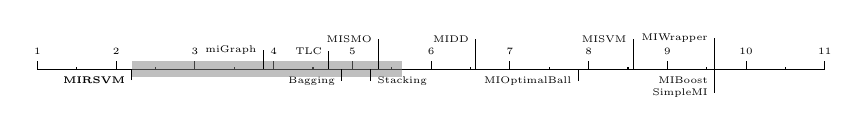
\begin{tikzpicture}
\draw (1,0) -- (11,0);
\foreach \x in {1,2,3,4,5,6,7,8,9,10,11} {
\draw (\x, 0) -- ++(0,.1) node [above,scale=0.7] {\tiny \x};
\ifthenelse{\x < 11}{\draw (\x+.5, 0) -- ++(0,.03);}{}
}

\coordinate (c0) at (2.2,0);
\coordinate (c1) at (3.8667,0);
\coordinate (c2) at (9.6,0);
\coordinate (c3) at (7.8667,0);
\coordinate (c4) at (6.5667,0);
\coordinate (c5) at (9.6,0);
\coordinate (c6) at (5.3333,0);
\coordinate (c7) at (8.5667,0);
\coordinate (c8) at (9.6,0);
\coordinate (c9) at (4.7,0);
\coordinate (c10) at (4.8667,0);
\coordinate (c11) at (5.2333,0);

\node (l0) at (c0) [below left=.01cm and 0cm, align=right,scale=0.7] {\tiny \textbf{MIRSVM}};
\node (l1) at (c1) [above left=.1cm and 0cm, align=right,scale=0.7] {\tiny miGraph};
\node (l2) at (c2) [below left=.01cm and 0cm, align=right,scale=0.7] {\tiny MIBoost};
\node (l3) at (c3) [below left=.01cm and 0cm, align=right,scale=0.7] {\tiny MIOptimalBall};
\node (l4) at (c4) [above left=.25cm and 0cm, align=right,scale=0.7] {\tiny MIDD};
\node (l5) at (c5) [above left=.25cm and 0cm, align=right,scale=0.7] {\tiny MIWrapper};
\node (l6) at (c6) [above left=.25cm and 0cm, align=right,scale=0.7] {\tiny MISMO};
\node (l7) at (c7) [above left=.25cm and 0cm, align=right,scale=0.7] {\tiny MISVM};
\node (l8) at (c8) [below left=.16cm and 0cm, align=right,scale=0.7] {\tiny SimpleMI};
\node (l9) at (c9) [above left=.1cm and 0cm, align=right,scale=0.7] {\tiny TLC};
\node (l10) at (c10) [below left=.01cm and 0cm, align=right,scale=0.7] {\tiny Bagging};
\node (l11) at (c11) [below right=.01cm and 0cm, align=left,scale=0.7] {\tiny Stacking};

\fill[fill=gray,fill opacity=0.5] (2.2,-0.1) rectangle (5.635,0.1);

\foreach \x in {0,1,2,3,4,5,6,7,8,9,10,11} {
\draw (l\x) -| (c\x);
};
\end{tikzpicture}}\vspace{-1.3em}
\captionof{figure}{\small Bonferroni-Dunn test for Accuracy}\label{fig:BonfDunnacc}\vspace{-1.3em}
\captionof{table}{\small Holm and Wilcoxon tests for Accuracy}\label{tab:MIstatacc}
\vspace{-1em}
\scriptsize
\resizebox{0.95\textwidth}{!}{\begin{tabular}{lccccccccccc}
\noalign{\smallskip}\hline\noalign{\smallskip}
MIRSVM vs. &miGraph &MIBoost &MIOptimalBall &MIDD &MIWrapper &MISMO &MISVM &SimpleMI &TLC &Bagging &Stacking \\
\noalign{\smallskip}\hline\noalign{\smallskip}
Holm $p$-value &0.0500 &0.0045 &0.0071 &0.0083 &0.0050 &0.0100 &0.0063 &0.0056 &0.0250 &0.0167 &0.0125 \\\noalign{\smallskip}\hline\noalign{\smallskip}
Wilcoxon $p$-value &0.0279 &0.0001 &0.0001 &0.0001 &0.0001 &0.0001 &0.0001 &0.0001 &0.0067 & 0.3028 &0.0103 \\
Wilcoxon R$^+$ &98.500 &120.00 &119.00 &120.00 &120.00 &120.00 &120.00 &120.00 &106.00 &79.000 &104.00 \\
Wilcoxon R$^-$ &21.500 & 0.0000 &1.0000 & 0.0000 &0.0000 &0.0000 &0.0000 &0.0000 &14.000 &41.000 &16.000 \\
\noalign{\smallskip}\hline\noalign{\smallskip}
\end{tabular}}
\end{table}
\subsection{Accuracy}
The results for accuracy indicate that the bag-based and ensemble learners perform better than the instance-based and wrapper methods. MIRSVM achieves the best accuracy over $5$ of the $15$ datasets with a competitive average against miGraph, Bagging, Stacking, and TLC. Note that MIRSVM performs better than MISVM for all datasets, indicating that using representatives from each bag and limiting the number of support vectors per negative bag improves the classification performance. The instance-level classifiers and wrapper methods, such as MIBoost, MIWrapper, and SimpleMI perform the worst. This behavior emphasizes the importance of not making prior assumptions about the positive bags' distributions. 

Figure~\ref{fig:BonfDunnacc} and Table~\ref{tab:statacc} show the results for the statistical analysis on the accuracy results. The algorithms with ranking higher than $5.63$ (MIRSVM rank + Bonferroni-Dunn critical value), to the right of the gray bar in Figure~\ref{fig:BonfDunnacc}, perform statistically worse than MIRSVM. Table~\ref{tab:statacc} shows the $p$-values of the Holm and Wilcoxon tests and their results complement one another. Holm's procedure rejects those hypotheses having a $p$-value $\leq 0.01$, thus indicating that MIRSVM performs significantly better than all methods except miGraph, Bagging, Stacking, and TLC. The Wilcoxon $p$-values show significant differences exist among all algorithms except miGraph, Bagging, and Stacking. They also show that MIRSVM has significantly better accuracy than MIBoost, MIOptimalBall, MIDD, MIWrapper, MISMO, MISVM, and SimpleMI, each having respectively small $p$-values, highlighting MIRSVM's superior classification accuracy. 

\subsection{Precision \& Recall}
Precision and recall are conflicting metrics that must be evaluated together in order to observe their behavior, since they are both used to measure relevance. The results for MIWrapper and SimpleMI indicate that they are unstable classifiers, exhibiting extreme variance in behavior, making them unsuitable for real-world applications. It is also interesting to analyze the performance on the mutagenesis datasets which have a larger number of positive bags than negative, where MISVM, MIBoost, MIWrapper, and SimpleMI predict all bags as negative. Additionally, while MISMO obtains unbiased results on these datasets, MIRSVM significantly outperforms it over both precision and recall, achieving a better trade-off.  
\begin{table}[H]
\small
\caption{\small Precision for MI classifiers}\label{tab:preResults}
\resizebox{0.95\textwidth}{!}{\begin{tabular}{l@{\extracolsep{\fill}}ccccccccccccc}
\noalign{\smallskip}\hline\noalign{\smallskip}
Datasets &MIRSVM & miGraph & MIBoost &MIOptimalBall &MIDD &MIWrapper &MISMO &MISVM &SimpleMI &TLC &Bagging &Stacking \\
\noalign{\smallskip}\hline\noalign{\smallskip}
suramin &0.7778 &0.7778 &\textbf{1.0000} &\textbf{1.0000} &0.2857 &\textbf{1.0000} &\textbf{1.0000} &0.5000 &\textbf{1.0000} &0.6429 &0.6514 &0.4000 &  \\
eastWest &0.7143 &0.7000 &0.5000 &0.8750 &0.5882 &0.5000 &0.7429 &\textbf{1.0000} &0.5000 &0.6053 &0.6053 &0.4444 &  \\
westEast &0.7272 &0.7273 &0.5000 &0.2727 &0.4600 &0.5000 &0.6939 &0.3600 &0.5000 &0.5581 &\textbf{0.9729} &0.6038 &  \\
musk1 &0.8519 &0.7778 &\textbf{1.0000} &0.9286 &0.9048 &\textbf{1.0000} &0.8049 &0.8108 &\textbf{1.0000} &0.8478 &0.8817 &0.8478 &  \\
musk2 &0.7059 &0.7826 &0.6139 &0.7826 &0.7576 &0.6139 &0.7424 &0.7538 &0.6139 &0.7400 &\textbf{0.9138} &0.7164 &  \\
webmining &0.7500 &\textbf{1.0000} &0.8142 &0.8173 &0.8142 &0.8142 &0.8936 &\textbf{1.0000} &0.8142 &0.8817 &0.9462 &0.8500 &  \\
trx &\textbf{1.0000} &0.8571 &0.8705 &0.9306 &0.9191 &0.8705 &0.8705 &0.8705 &0.8705 &0.9138 &0.6747 &0.9011 &  \\
mutagenesis-atoms &0.7872 &0.7985 &\textbf{1.0000} &0.4630 &0.6111 &\textbf{1.0000} &0.5439 &\textbf{1.0000} &\textbf{1.0000} &0.7059 &0.7059 &0.6667 &  \\
mutagenesis-bonds &0.8468 &0.8195 &\textbf{1.0000} &0.5385 &0.7500 &\textbf{1.0000} &0.6812 &\textbf{1.0000} &\textbf{1.0000} &0.7857 &0.7857 &0.8333 &  \\
mutagenesis-chains &0.8571 &0.8116 &\textbf{1.0000} &0.5091 &0.7059 &\textbf{1.0000} &0.7759 &\textbf{1.0000} &\textbf{1.0000} &0.7705 &0.7705 &0.7581 &  \\
tiger &0.7365 &0.7323 &0.5000 &0.5000 &0.6944 &0.5000 &0.7444 &0.7802 &0.5000 &0.6514 &\textbf{0.8000} &0.7320 &  \\
elephant &0.8576 &\textbf{0.8750} &0.5000 &0.5000 &0.7959 &0.5000 &0.8444 &0.7679 &0.5000 &0.8000 &0.5581 &0.8283 &  \\
fox &0.6040 &0.6275 &0.5000 &0.5000 &0.5833 &0.5000 &0.5287 &0.4854 &0.5000 &0.6747 &\textbf{0.8478} &0.6705 &  \\
component &\textbf{0.9866} &0.7782 &0.8649 &0.8778 &0.8902 &0.8649 &0.8958 &0.8696 &0.8649 &0.9462 &0.6429 &0.9449 &  \\
function &0.8459 &0.6775 &0.9155 &0.9202 &0.9317 &0.9155 &0.9376 &0.9197 &0.9155 &\textbf{0.9729} &0.7400 &0.9726 &  \\
\noalign{\smallskip}\hline\noalign{\smallskip}
Average &0.8033 &0.7828 &0.7719 &0.6944 &0.7128 &0.7719 &0.7800 &\textbf{0.8079} &0.7719 &0.7665 &0.7665 &0.7447 &  \\
Rank &\textbf{5.3333} &6.1333 &7.1000 &7.3333 &7.3667 &7.1000 &5.8667 &5.8667 &7.1000 &5.9000 &6.3333 &6.5667 &  \\
\noalign{\smallskip}\hline
\end{tabular}}
\centering
\resizebox{0.95\textwidth}{!}{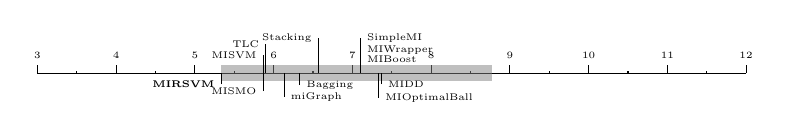
\begin{tikzpicture}
\draw (3,0) -- (12,0);
\foreach \x in {3,4,5,6,7,8,9,10,11,12} {
\draw (\x, 0) -- ++(0,.1) node [above,scale=0.7] {\tiny \x};
\ifthenelse{\x < 12}{\draw (\x+.5, 0) -- ++(0,.03);}{}
}

\coordinate (c0) at (5.3333,0);
\coordinate (c1) at (6.1333,0);
\coordinate (c2) at (7.1,0);
\coordinate (c3) at (7.3333,0);
\coordinate (c4) at (7.3667,0);
\coordinate (c5) at (7.1,0);
\coordinate (c6) at (5.8667,0);
\coordinate (c7) at (5.8667,0);
\coordinate (c8) at (7.1,0);
\coordinate (c9) at (5.9,0);
\coordinate (c10) at (6.3333,0);
\coordinate (c11) at (6.5667,0);

\node (l0) at (c0) [below left=.01cm and 0cm, align=right,scale=0.7] {\tiny \textbf{MIRSVM}};
\node (l1) at (c1) [below right=.16cm and 0cm, align=left,scale=0.7] {\tiny miGraph};
\node (l2) at (c2) [above right=.05cm and 0cm, align=left,scale=0.7] {\tiny MIBoost};
\node (l3) at (c3) [below right=.17cm and 0cm, align=left,scale=0.7] {\tiny MIOptimalBall};
\node (l4) at (c4) [below right=.01cm and 0cm, align=left,scale=0.7] {\tiny MIDD};
\node (l5) at (c5) [above right=.15cm and 0cm, align=left,scale=0.7] {\tiny MIWrapper};
\node (l6) at (c6) [below left=.1cm and 0cm, align=right,scale=0.7] {\tiny MISMO};
\node (l7) at (c7) [above left=.1cm and 0cm, align=right,scale=0.7] {\tiny MISVM};
\node (l8) at (c8) [above right=.3cm and 0cm, align=left,scale=0.7] {\tiny SimpleMI};
\node (l9) at (c9) [above left=.24cm and 0cm, align=right,scale=0.7] {\tiny TLC};
\node (l10) at (c10) [below right=.01cm and 0cm, align=left,scale=0.7] {\tiny Bagging};
\node (l11) at (c11) [above left=.3cm and 0cm, align=right,scale=0.7] {\tiny Stacking};

\fill[fill=gray,fill opacity=0.5] (5.3333,-0.1) rectangle (8.7683,0.1);

\foreach \x in {0,1,2,3,4,5,6,7,8,9,10,11} {
\draw (l\x) -| (c\x);};
\end{tikzpicture}}\vspace{-1.3em}
\captionof{figure}{\small Bonferroni-Dunn test for Precision}\label{fig:BonfDunnprec}\vspace{-1.3em}
\captionof{table}{\small Holm and Wilcoxon tests for Precision}\label{tab:statprec}
\vspace{-1em}
\scriptsize
\resizebox{0.9\textwidth}{!}{\begin{tabular}{lccccccccccc}
\noalign{\smallskip}\hline\noalign{\smallskip}
MIRSVM vs. &miGraph &MIBoost &MIOptimalBall &MIDD &MIWrapper &MISMO &MISVM &SimpleMI &TLC &Bagging &Stacking \\
\noalign{\smallskip}\hline\noalign{\smallskip}
Holm $p$-value &0.0125 &0.0056 &0.0050 &0.0045 &0.0063 &0.0250 &0.0500 &0.0071 &0.0167 &0.0100 &0.0083 \\\noalign{\smallskip}\hline\noalign{\smallskip}
Wilcoxon $p$-value & 0.4212 & 0.5614 &0.0946 &0.0256 & 0.5614 & 0.4212 & 0.8039 & 0.5614 &0.1354 & 0.4543 &0.1354 \\
Wilcoxon R$^+$ &75.000 &71.000 &90.000 &99.000 &71.000 &75.000 &55.000 &71.000 &87.000 &74.000 &87.000 \\
Wilcoxon R$^-$ &45.000 &49.000 &30.000 &21.000 &49.000 &45.000 &65.000 &49.000 &33.000 &46.000 &33.000 \\
\noalign{\smallskip}\hline\noalign{\smallskip}
\end{tabular}}
\small \centering
\captionof{table}{\small Recall for MI classifiers}\label{tab:recResults}
\resizebox{0.95\textwidth}{!}{\begin{tabular}{l@{\extracolsep{\fill}}ccccccccccccc}
\noalign{\smallskip}\hline\noalign{\smallskip}
Datasets &MIRSVM & miGraph & MIBoost &MIOptimalBall &MIDD &MIWrapper &MISMO &MISVM &SimpleMI &TLC &Bagging &Stacking \\
\noalign{\smallskip}\hline\noalign{\smallskip}
suramin &\textbf{1.0000} &\textbf{1.0000} &0.0000 &0.4500 &0.1000 &0.0000 &0.4500 &0.5000 &0.0000 &0.4500 &0.7100 &0.3333 &  \\
eastWest &\textbf{1.0000} &0.7000 &0.7000 &0.5250 &0.7500 &0.7000 &0.6500 &0.1250 &\textbf{1.0000} &0.5750 &0.5750 &0.4000 &  \\
westEast &0.8000 &0.8000 &0.9000 &0.1500 &0.5750 &0.9000 &0.8500 &0.2250 &\textbf{1.0000} &0.6000 &0.9892 &0.8000 &  \\
musk1 &\textbf{0.9787} &0.8936 &0.0000 &0.5778 &0.8444 &0.0000 &0.7333 &0.6667 &0.0000 &0.8667 &0.8913 &0.8667 &  \\
musk2 &0.9231 &0.4615 &\textbf{1.0000} &0.8710 &0.8065 &\textbf{1.0000} &0.7903 &0.7903 &\textbf{1.0000} &0.5968 &0.9464 &0.7742 &  \\
webmining &0.2857 &0.0000 &\textbf{1.0000} &0.9239 &\textbf{1.0000} &\textbf{1.0000} &0.9130 &0.6196 &\textbf{1.0000} &0.8913 &0.9815 &0.9239 &  \\
trx &0.4833 &0.2400 &\textbf{1.0000} &0.9583 &0.9464 &\textbf{1.0000} &\textbf{1.0000} &\textbf{1.0000} &\textbf{1.0000} &0.9464 &0.5600 &0.9762 &  \\
mutagenesis-atoms &\textbf{0.8880} &0.8560 &0.0000 &0.3968 &0.3492 &0.0000 &0.4921 &0.0000 &0.0000 &0.5714 &0.5714 &0.5714 &  \\
mutagenesis-bonds &\textbf{0.8960} &0.8720 &0.0000 &0.5556 &0.4762 &0.0000 &0.7460 &0.0000 &0.0000 &0.6984 &0.6984 &0.7143 &  \\
mutagenesis-chains &\textbf{0.9120} &0.8960 &0.0000 &0.4444 &0.5714 &0.0000 &0.7143 &0.0000 &0.0000 &0.7460 &0.7460 &0.7460 &  \\
tiger &0.8700 &0.9300 &0.5000 &\textbf{1.0000} &0.7500 &0.5000 &0.6700 &0.7100 &\textbf{1.0000} &0.7100 &0.8000 &0.7100 &  \\
elephant &0.9100 &0.7700 &0.6000 &\textbf{1.0000} &0.7800 &0.6000 &0.7600 &0.8600 &\textbf{1.0000} &0.8000 &0.6000 &0.8200 &  \\
fox &0.9000 &0.6400 &0.7000 &\textbf{1.0000} &0.5600 &0.7000 &0.4600 &0.8300 &\textbf{1.0000} &0.5600 &0.8667 &0.5900 &  \\
component &0.5839 &0.5225 &\textbf{1.0000} &0.9867 &0.9797 &\textbf{1.0000} &0.9967 &\textbf{1.0000} &\textbf{1.0000} &0.9815 &0.4500 &0.9826 &  \\
function &0.5327 &0.5643 &\textbf{1.0000} &0.9919 &0.9840 &\textbf{1.0000} &0.9983 &0.9994 &\textbf{1.0000} &0.9892 &0.5968 &0.9894 &  \\
\noalign{\smallskip}\hline\noalign{\smallskip}
Average &\textbf{0.7976} &0.6764 &0.5600 &0.7221 &0.6982 &0.5600 &0.7483 &0.5551 &0.6667 &0.7322 &0.7322 &0.7465 &  \\
Rank &4.8667 &6.5667 &6.8667 &6.3333 &7.3667 &6.8667 &6.7000 &7.4333 &\textbf{4.8333} &7.3667 &6.0667 &6.7333 &  \\
\noalign{\smallskip}\hline
\end{tabular}}
\resizebox{0.95\textwidth}{!}{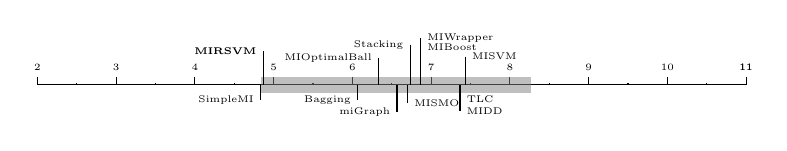
\begin{tikzpicture}
\draw (2,0) -- (11,0);
\foreach \x in {2,3,4,5,6,7,8,9,10,11,11} {
\draw (\x, 0) -- ++(0,.1) node [above,scale=0.7] {\tiny \x};
\ifthenelse{\x < 11}{\draw (\x+.5, 0) -- ++(0,.03);}{}
}

\coordinate (c0) at (4.8667,0);
\coordinate (c1) at (6.5667,0);
\coordinate (c2) at (6.8667,0);
\coordinate (c3) at (6.3333,0);
\coordinate (c4) at (7.3667,0);
\coordinate (c5) at (6.8667,0);
\coordinate (c6) at (6.7,0);
\coordinate (c7) at (7.4333,0);
\coordinate (c8) at (4.8333,0);
\coordinate (c9) at (7.3667,0);
\coordinate (c10) at (6.0667,0);
\coordinate (c11) at (6.7333,0);

\node (l0) at (c0) [above left=.3cm and 0cm, align=right,scale=0.7] {\tiny \textbf{MIRSVM}};
\node (l1) at (c1) [below left=.2cm and 0cm, align=right,scale=0.7] {\tiny miGraph};
\node (l2) at (c2) [above right=.35cm and 0cm, align=left,scale=0.7] {\tiny MIBoost};
\node (l3) at (c3) [above left=.2cm and 0cm, align=right,scale=0.7] {\tiny MIOptimalBall};
\node (l4) at (c4) [below right=.2cm and 0cm, align=left,scale=0.7] {\tiny MIDD};
\node (l5) at (c5) [above right=.45cm and 0cm, align=left,scale=0.7] {\tiny MIWrapper};
\node (l6) at (c6) [below right=.1cm and 0cm, align=left,scale=0.7] {\tiny MISMO};
\node (l7) at (c7) [above right=.23cm and 0cm, align=left,scale=0.7] {\tiny MISVM};
\node (l8) at (c8) [below left=.05cm and 0cm, align=right,scale=0.7] {\tiny SimpleMI};
\node (l9) at (c9) [below right=.05cm and 0cm, align=left,scale=0.7] {\tiny TLC};
\node (l10) at (c10) [below left=.05cm and 0cm, align=right,scale=0.7] {\tiny Bagging};
\node (l11) at (c11) [above left=.37cm and 0cm, align=right,scale=0.7] {\tiny Stacking};

\fill[fill=gray,fill opacity=0.5] (4.8333,-0.1) rectangle (8.2683,0.1);

\foreach \x in {0,1,2,3,4,5,6,7,8,9,10,11} {
\draw (l\x) -| (c\x);};
\end{tikzpicture}}\vspace{-1.3em}
\captionof{figure}{\small Bonferroni-Dunn test for Recall}\label{fig:BonfDunnrec}\vspace{-1.3em}
\captionof{table}{\small Holm and Wilcoxon tests for Recall}\label{tab:statrec}
\vspace{-1em}
\scriptsize
\centering
\resizebox{0.9\textwidth}{!}{\begin{tabular}{lccccccccccc}
\noalign{\smallskip}\hline\noalign{\smallskip}
MIRSVM vs. &miGraph &MIBoost &MIOptimalBall &MIDD &MIWrapper &MISMO &MISVM &SimpleMI &TLC &Bagging &Stacking \\
\noalign{\smallskip}\hline\noalign{\smallskip}
Holm $p$-value &0.0125 &0.0063 &0.0167 &0.0050 &0.0071 &0.0100 &0.0045 &0.0500 &0.0056 &0.0250 &0.0083 \\\noalign{\smallskip}\hline\noalign{\smallskip}
Wilcoxon $p$-value &0.0060 & 0.2077 & 0.5614 & 0.4543 & 0.2077 & 0.6387 &0.1070 & 0.6603 & 0.5995 &0.1354 & 0.5721 \\
Wilcoxon R$^+$ &106.50 &83.000 &71.000 &74.000 &83.000 &69.000 &89.000 &60.000 &70.000 &87.000 &62.000 \\
Wilcoxon R$^-$ &13.500 &37.000 &49.000 &46.000 &37.000 &51.000 &31.000 &45.000 &50.000 &33.000 &43.000 \\
\noalign{\smallskip}\hline\noalign{\smallskip}
\end{tabular}}
\end{table}

Figure~\ref{fig:BonfDunnprec} and~\ref{fig:BonfDunnrec} show that there are no significant differences between the precision and recall results obtained by all algorithms. Note, MIRSVM outperforms both ensemble methods according to recall, despite them exhibiting good accuracy and precision, indicating they are strongly conservative towards predicting positive bags. Holm's test indicates significant differences exist between MIRSVM and all algorithms except miGraph, MISMO, MISVM, and TLC for precision, and all the above along with SimpleMI, MIOptimalBall, and Bagging for recall. The Wilcoxon test does not reflect significant differences for precision, does for recall. The tests are severely biased due to the classifier's extreme unbalanced behavior, whereas MIRSVM demonstrates proper balance of the precision-recall trade-off.

\subsection{Cohen's Kappa Rate}
\begin{table}[b!]
\small
\caption{\small Cohen's Kappa Rate for MI classifiers}\label{tab:kappaResults}
\resizebox{0.95\textwidth}{!}{\begin{tabular}{lccccccccccccc}
\noalign{\smallskip}\hline\noalign{\smallskip}
Datasets &MIRSVM & miGraph & MIBoost &MIOptimalBall &MIDD &MIWrapper &MISMO &MISVM &SimpleMI &TLC &Bagging &Stacking \\
\noalign{\smallskip}\hline\noalign{\smallskip}
suramin &\textbf{0.6829} &\textbf{0.6829} &0.0000 &0.4500 &-0.1500 &0.0000 &0.4500 &0.0000 &0.0000 &0.2000 &0.3300 &-0.0964 &  \\
eastWest &\textbf{0.6000} &0.4000 &0.0000 &0.4500 &0.2250 &0.0000 &0.4250 &0.1250 &0.0000 &0.2000 &0.2000 &-0.1000 &  \\
westEast &0.5000 &0.5000 &0.0000 &-0.2500 &-0.1000 &0.0000 &0.4750 &-0.1750 &0.0000 &0.1250 &\textbf{0.7529} &0.2750 &  \\
musk1 &\textbf{0.8036} &0.6290 &0.0000 &0.5396 &0.7604 &0.0000 &0.5642 &0.5197 &0.0000 &0.7174 &0.3744 &0.7174 &  \\
musk2 &\textbf{0.6540} &0.4123 &0.0000 &0.5031 &0.4039 &0.0000 &0.3613 &0.3856 &0.0000 &0.2492 &0.3858 &0.2940 &  \\
webmining &0.3468 &0.0000 &0.0000 &0.0246 &0.0000 &0.0000 &0.4535 &0.3771 &0.0000 &0.3744 &\textbf{0.6945} &0.2458 &  \\
trx &0.2100 &0.3375 &0.0000 &\textbf{0.5228} &0.4224 &0.0000 &0.0000 &0.0000 &0.0000 &0.3858 &0.2900 &0.3364 &  \\
mutagenesis-atoms &\textbf{0.5395} &0.4431 &0.0000 &0.1709 &0.2654 &0.0000 &0.2909 &0.0000 &0.0000 &0.4738 &0.4738 &0.4431 &  \\
mutagenesis-bonds &0.5699 &0.5070 &0.0000 &0.3131 &0.4356 &0.0000 &0.5569 &0.0000 &0.0000 &0.6195 &0.6195 &\textbf{0.6659} &  \\
mutagenesis-chains &0.6303 &0.5094 &0.0000 &0.2359 &0.4738 &0.0000 &0.6225 &0.0000 &0.0000 &\textbf{0.6391} &\textbf{0.6391} &0.6285 &  \\
tiger &0.5500 &0.5900 &0.0000 &0.0000 &0.4200 &0.0000 &0.4400 &0.5100 &0.0000 &0.3300 &\textbf{0.6000} &0.4500 &  \\
elephant &\textbf{0.7000} &0.6600 &0.0000 &0.0000 &0.5800 &0.0000 &0.6200 &0.6000 &0.0000 &0.6000 &0.1250 &0.6500 &  \\
fox &0.3100 &0.2600 &0.0000 &0.0000 &0.1600 &0.0000 &0.0500 &-0.0500 &0.0000 &0.2900 &\textbf{0.7174} &0.3000 &  \\
component &0.6644 &0.5795 &0.0000 &0.1613 &0.2836 &0.0000 &0.3656 &0.0675 &0.0000 &\textbf{0.6945} &0.2000 &0.6906 &  \\
function &0.6292 &0.5838 &0.0000 &0.0966 &0.2801 &0.0000 &0.4083 &0.0933 &0.0000 &\textbf{0.7529} &0.2492 &0.7507 &  \\
\noalign{\smallskip}\hline\noalign{\smallskip}
Average &\textbf{0.5594} &0.4730 &0.0000 &0.2145 &0.2973 &0.0000 &0.4056 &0.1635 &0.0000 &0.4434 &0.4434 &0.4167 &  \\
Rank &\textbf{2.6333} &4.2000 &10.1667 &7.0000 &6.5333 &10.1667 &5.2333 &8.3667 &10.1667 &4.2667 &4.2667 &5.0000 &  \\
\noalign{\smallskip}\hline\noalign{\smallskip}
\end{tabular}}
\centering
\resizebox{0.95\textwidth}{!}{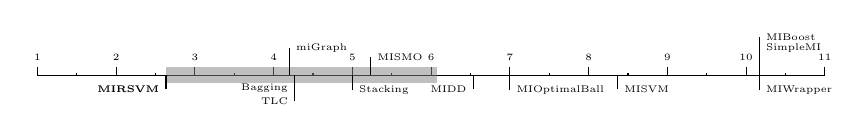
\begin{tikzpicture}
\draw (1,0) -- (11,0);
\foreach \x in {1,2,3,4,5,6,7,8,9,10,11} {
\draw (\x, 0) -- ++(0,.1) node [above,scale=0.7] {\tiny \x};
\ifthenelse{\x < 11}{\draw (\x+.5, 0) -- ++(0,.03);}{}
}

\coordinate (c0) at (2.6333,0);
\coordinate (c1) at (4.2,0);
\coordinate (c2) at (10.1667,0);
\coordinate (c3) at (7,0);
\coordinate (c4) at (6.5333,0);
\coordinate (c5) at (10.1667,0);
\coordinate (c6) at (5.2333,0);
\coordinate (c7) at (8.3667,0);
\coordinate (c8) at (10.1667,0);
\coordinate (c9) at (4.2667,0);
\coordinate (c10) at (4.2667,0);
\coordinate (c11) at (5,0);

\node (l0) at (c0) [below left=.05cm and 0cm, align=right,scale=0.7] {\tiny \textbf{MIRSVM}};
\node (l1) at (c1) [above right=.2cm and 0cm, align=left,scale=0.7] {\tiny miGraph};
\node (l2) at (c2) [above right=.35cm and 0cm, align=right,scale=0.7] {\tiny MIBoost};
\node (l3) at (c3) [below right=.05cm and 0cm, align=left,scale=0.7] {\tiny MIOptimalBall};
\node (l4) at (c4) [below left=.05cm and 0cm, align=right,scale=0.7] {\tiny MIDD};
\node (l5) at (c5) [below right=.05cm and 0cm, align=left,scale=0.7] {\tiny MIWrapper};
\node (l6) at (c6) [above right=.1cm and 0cm, align=left,scale=0.7] {\tiny MISMO};
\node (l7) at (c7) [below right=.05cm and 0cm, align=left,scale=0.7] {\tiny MISVM};
\node (l8) at (c8) [above right=.2cm and 0cm, align=left,scale=0.7] {\tiny SimpleMI};
\node (l9) at (c9) [below left=.2cm and 0cm, align=right,scale=0.7] {\tiny TLC};
\node (l10) at (c10) [below left=.02cm and 0cm, align=right,scale=0.7] {\tiny Bagging};
\node (l11) at (c11) [below right=.05cm and 0cm, align=right,scale=0.7] {\tiny Stacking};

\fill[fill=gray,fill opacity=0.5] (2.6333,-0.1) rectangle (6.0683,0.1);

\foreach \x in {0,1,2,3,4,5,6,7,8,9,10,11} {
\draw (l\x) -| (c\x);
};
\end{tikzpicture}}\vspace{-1.3em}
\captionof{figure}{\small Bonferroni-Dunn test for Cohen's Kappa rate}\label{fig:BonfDunnkappa}
\vspace{-1.3em}
\captionof{table}{\small Holm and Wilcoxon tests for Cohen's Kappa rate}\label{tab:statkappa}
\vspace{-1em}
\scriptsize \centering
\resizebox{0.9\textwidth}{!}{\begin{tabular}{lccccccccccc}
\noalign{\smallskip}\hline\noalign{\smallskip}
MIRSVM vs. &miGraph &MIBoost &MIOptimalBall &MIDD &MIWrapper &MISMO &MISVM &SimpleMI &TLC &Bagging &Stacking \\
\noalign{\smallskip}\hline\noalign{\smallskip}
Holm $p$-value &0.0500 &0.0045 &0.0071 &0.0083 &0.0050 &0.0100 &0.0063 &0.0056 &0.0167 &0.0250 &0.0125 \\\noalign{\smallskip}\hline\noalign{\smallskip}
Wilcoxon $p$-value &0.0121 &0.0001 &0.0012 &0.0012 &0.0001 &0.0006 &0.0001 &0.0001 &0.1205 & 0.2077 &0.0946 \\
Wilcoxon R$^+$ &91.500 &120.00 &113.00 &113.00 &120.00 &115.00 &119.00 &120.00 &88.000 &83.000 &90.000 \\
Wilcoxon R$^-$ &13.500 &0.0000 &7.0000 &7.0000 &0.0000 &5.0000 &1.0000 &0.0000 &32.000 &37.000 &30.000 \\
\noalign{\smallskip}\hline\noalign{\smallskip}
\end{tabular}}
\end{table}
Table~\ref{tab:kappaResults} shows the Cohen's Kappa rate results obtained by the algorithms. These results support the accuracy achieved by the algorithms, in the sense that the instance-based and wrapper methods perform worse than bag-based and ensemble learners. MIRSVM's kappa values all fall within the range ($0.5$-$1$], indicating that its merit as a classifier agrees with the class distribution and is not random. Note that MIOptimalBall, MIDD, MISVM, MISMO, and Stacking contain some negative kappa values, indicating performance worse than the default-hypothesis. MIBoost, SimpleMI, and MIWrapper are shown to randomly classify all $15$ datasets. Figure~\ref{fig:BonfDunnkappa} and Table~\ref{tab:statkappa} show the results of the statistical analysis on the Cohen's Kappa Rate results. The Holm and Wilcoxon procedures reflect results similar to the Bonferroni-Dunn test, where MIRSVM performs significantly better than MIOptimalBall, MIDD, MISVM, MIWrapper, MIBoost, and SimpleMI, having $p$-values $< 0.01$. This supports MIRSVM's performance as a competitive classifier.

\subsection{Area Under ROC Curve}
\begin{table}[b!]
\small \centering
\caption{\small AUC for MI classifiers}\label{tab:aucResults}
\resizebox{0.95\textwidth}{!}{\begin{tabular}{lccccccccccccc}
\hline\noalign{\smallskip}
Datasets &MIRSVM & miGraph & MIBoost &MIOptimalBall &MIDD &MIWrapper &MISMO &MISVM &SimpleMI &TLC &Bagging &Stacking \\
\hline\noalign{\smallskip}
suramin &\textbf{0.8333} &\textbf{0.8333} &0.5000 &0.7250 &0.4250 &0.5000 &0.7250 &0.5000 &0.5000 &0.6000 &0.6650 &0.4524 &  \\
eastWest &\textbf{0.8000} &0.7000 &0.5000 &0.7250 &0.6125 &0.5000 &0.7125 &0.5625 &0.5000 &0.6000 &0.6000 &0.4500 &  \\
westEast &0.7500 &0.7500 &0.5000 &0.3750 &0.4500 &0.5000 &0.7375 &0.4125 &0.5000 &0.5625 &\textbf{0.8456} &0.6375 &  \\
musk1 &\textbf{0.9005} &0.8135 &0.5000 &0.7676 &0.8797 &0.5000 &0.7816 &0.7589 &0.5000 &0.8589 &0.6837 &0.8589 &  \\
musk2 &\textbf{0.8406} &0.6904 &0.5000 &0.7432 &0.6981 &0.5000 &0.6772 &0.6900 &0.5000 &0.6317 &0.6732 &0.6435 &  \\
webmining &0.6320 &0.5000 &0.5000 &0.5096 &0.5000 &0.5000 &0.7184 &0.8098 &0.5000 &0.6837 &\textbf{0.8123} &0.6048 &  \\
trx &0.6500 &0.6170 &0.5000 &\textbf{0.7392} &0.6932 &0.5000 &0.5000 &0.5000 &0.5000 &0.6732 &0.6450 &0.6281 &  \\
mutagenesis-atoms &0.7106 &0.7137 &0.5000 &0.5824 &0.6186 &0.5000 &0.6420 &0.5000 &0.5000 &\textbf{0.7257} &\textbf{0.7257} &0.7137 &  \\
mutagenesis-bonds &0.7856 &0.7455 &0.5000 &0.6578 &0.6981 &0.5000 &0.7850 &0.5000 &0.5000 &0.8012 &0.8012 &\textbf{0.8211} &  \\
mutagenesis-chains &\textbf{0.8252} &0.7417 &0.5000 &0.6142 &0.7257 &0.5000 &0.8051 &0.5000 &0.5000 &0.8170 &0.8170 &0.8130 &  \\
tiger &0.7750 &0.7950 &0.5000 &0.5000 &0.7100 &0.5000 &0.7200 &0.7550 &0.5000 &0.6650 &\textbf{0.8000} &0.7250 &  \\
elephant &0.8200 &\textbf{0.8300} &0.5000 &0.5000 &0.7900 &0.5000 &0.8100 &0.8000 &0.5000 &0.8000 &0.5625 &0.8250 &  \\
fox &0.6550 &0.6300 &0.5000 &0.5000 &0.5800 &0.5000 &0.5250 &0.4750 &0.5000 &0.6450 &\textbf{0.8589} &0.6500 &  \\
component &0.7855 &0.7496 &0.5000 &0.5536 &0.6033 &0.5000 &0.6272 &0.5201 &0.5000 &\textbf{0.8123} &0.6000 &0.8081 &  \\
function &0.7563 &0.7698 &0.5000 &0.5298 &0.6015 &0.5000 &0.6391 &0.5268 &0.5000 &\textbf{0.8456} &0.6317 &0.8434 &  \\
\noalign{\smallskip}\hline\noalign{\smallskip}
Average &\textbf{0.7680} &0.7253 &0.5000 &0.6015 &0.6390 &0.5000 &0.6937 &0.5874 &0.5000 &0.7148 &0.7148 &0.6983 &  \\
Rank &\textbf{2.7667} &4.2667 &10.1667 &7.0000 &6.5333 &10.1667 &5.2333 &8.2333 &10.1667 &4.2667 &4.2667 &4.9333 &  \\
\hline\noalign{\smallskip}
\end{tabular}}
\centering
\resizebox{0.95\textwidth}{!}{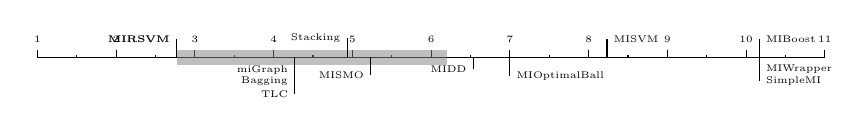
\begin{tikzpicture}
\draw (1,0) -- (11,0);
\foreach \x in {1,2,3,4,5,6,7,8,9,10,11} {
\draw (\x, 0) -- ++(0,.1) node [above,scale=0.7] {\tiny \x};
\ifthenelse{\x < 11}{\draw (\x+.5, 0) -- ++(0,.03);}{}
}

\coordinate (c0) at (2.7667,0);
\coordinate (c1) at (4.2667,0);
\coordinate (c2) at (10.1667,0);
\coordinate (c3) at (7,0);
\coordinate (c4) at (6.5333,0);
\coordinate (c5) at (10.1667,0);
\coordinate (c6) at (5.2333,0);
\coordinate (c7) at (8.2333,0);
\coordinate (c8) at (10.1667,0);
\coordinate (c9) at (4.2667,0);
\coordinate (c10) at (4.2667,0);
\coordinate (c11) at (4.9333,0);

\node (l0) at (c0) [above left=.1cm and 0cm, align=right,scale=0.7] {\tiny \textbf{MIRSVM}};
\node (l1) at (c1) [below left=.02cm and 0cm, align=right,scale=0.7] {\tiny miGraph};
\node (l2) at (c2) [above right=.1cm and 0cm, align=left,scale=0.7] {\tiny MIBoost};
\node (l3) at (c3) [below right=.1cm and 0cm, align=left,scale=0.7] {\tiny MIOptimalBall};
\node (l4) at (c4) [below left=.02cm and 0cm, align=right,scale=0.7] {\tiny MIDD};
\node (l5) at (c5) [below right=.01cm and 0cm, align=left,scale=0.7] {\tiny MIWrapper};
\node (l6) at (c6) [below left=.1cm and 0cm, align=right,scale=0.7] {\tiny MISMO};
\node (l7) at (c7) [above right=.1cm and 0cm, align=left,scale=0.7] {\tiny MISVM};
\node (l8) at (c8) [below right=.16cm and 0cm, align=left,scale=0.7] {\tiny SimpleMI};
\node (l9) at (c9) [below left=.34cm and 0cm, align=right,scale=0.7] {\tiny TLC};
\node (l10) at (c10) [below left=.16cm and 0cm, align=right,scale=0.7] {\tiny Bagging};
\node (l11) at (c11) [above left=.1cm and 0cm, align=right,scale=0.7] {\tiny Stacking};

\fill[fill=gray,fill opacity=0.5] (2.7667,-0.1) rectangle (6.2017,0.1);

\foreach \x in {0,1,2,3,4,5,6,7,8,9,10,11} {
\draw (l\x) -| (c\x);
};
\end{tikzpicture}}\vspace{-1.3em}
\captionof{figure}{\small Bonferroni-Dunn test for AUC}\label{fig:BonfDunnauc}\vspace{-1.3em}
\captionof{table}{\small Holm and Wilcoxon tests for AUC}\label{tab:statauc}
\vspace{-1em}
\scriptsize \centering
\resizebox{0.9\textwidth}{!}{\begin{tabular}{lccccccccccc}
\noalign{\smallskip}\hline\noalign{\smallskip}
MIRSVM vs. &miGraph &MIBoost &MIOptimalBall &MIDD &MIWrapper &MISMO &MISVM &SimpleMI &TLC &Bagging &Stacking \\
\noalign{\smallskip}\hline\noalign{\smallskip}
Holm $p$-value &0.0167 &0.0045 &0.0071 &0.0083 &0.0050 &0.0100 &0.0063 &0.0056 &0.0250 &0.0500 &0.0125 \\\noalign{\smallskip}\hline\noalign{\smallskip}
Wilcoxon $p$-value &0.0166 &0.0001 &0.0002 &0.0003 &0.0001 &0.0012 &0.0009 &0.0001 & 0.2523 & 0.3028 &0.0781 \\
Wilcoxon R$^+$ &90.000 &120.00 &118.00 &117.00 &120.00 &113.00 &114.00 &120.00 &81.000 &79.000 &91.500 \\
Wilcoxon R$^-$ &15.000 &0.0000 &2.0000 &3.0000 &0.0000 &7.0000 &6.0000 &0.0000 &39.000 &41.000 &28.500 \\
\noalign{\smallskip}\hline\noalign{\smallskip}
\end{tabular}}
\end{table}
Table~\ref{tab:aucResults} shows AUC results obtained by the algorithms, which complement the accuracy and kappa rate, emphasizing the better performance of bag-based methods. MIRSVM achieves the best AUC score on $5$ of the $15$ datasets, while MIBoost, SimpleMI, and MIWrapper obtain the worst results. Their AUC score indicates random predictor behavior, having values $= 0.5$. Bag-level methods all obtain scores between $0.7$ and $0.77$ indicating a high true positive rate and a low false positive rate, which is reflected by the precision and recall results. Figure~\ref{fig:BonfDunnauc} and Table~\ref{tab:statauc} show that MIRSVM performs significantly better than $6$ out of the $11$ competing algorithms. Holm's procedure indicates that significant differences exist between MIRSVM and all algorithms except miGraph, TLC, Bagging, and Stacking. MISVM's true positive rate could be affected because of the possible imbalance of support vectors from the positive and negative classes (favoring the negative). Note that the Wilcoxon $p$-values for MIWrapper, MIBoost, and SimpleMI are $0.0001$. 

\subsection{Overall Comparison}
\begin{table}[t!]
\small
\centering
\caption{\small Run Time (seconds) for MI classifiers}\label{tab:time}
\resizebox{0.95\textwidth}{!}{\begin{tabular}{lrrrrrrrrrrrrr}
\hline\noalign{\smallskip}
Datasets &MIRSVM & miGraph & MIBoost &MIOptimalBall &MIDD &MIWrapper &MISMO &MISVM &SimpleMI &TLC &Bagging &Stacking \\
\hline\noalign{\smallskip}
suramin &\textbf{0.1} &19.7 &8.8 &30.5 &7922.0 &9.5 &52.3 &333.9 &7.2 &35.5 &183.0 &90.6 &  \\
eastWest &\textbf{0.1} &3.0 &5.5 &9.4 &217.1 &6.3 &14.8 &21.4 &5.8 &15.4 &15.4 &15.2 &  \\
westEast &\textbf{0.1} &2.8 &6.5 &7.8 &79.7 &6.5 &14.7 &99.5 &6.0 &16.6 &12128.1 &10.8 &  \\
musk1 &\textbf{0.4} &56.8 &13.4 &32.1 &3542.6 &20.6 &89.7 &198.4 &11.1 &93.0 &86272.6 &759.5 &  \\
musk2 &\textbf{2.3} &452.3 &97.3 &782.9 &126016.8 &208.3 &1799.4 &26093.5 &16.1 &1772.2 &2229.3 &16759.0 &  \\
webmining &\textbf{300.6} &302.5 &45745.4 &60474.8 &47601.4 &68736.7 &51923.6 &105622.3 &2685.9 &86272.6 &9861.5 &592948.9 &  \\
trx &61.8 &2206.4 &17.6 &682.3 &339110.5 &19.3 &8670.3 &134622.1 &\textbf{7.4} &2229.3 &243.3 &11927.9 &  \\
mutagenesis-atoms &9.8 &193.1 &8.8 &99.2 &2623.0 &8.0 &55.0 &53.5 &\textbf{6.4} &44.0 &44.0 &153.9 &  \\
mutagenesis-bonds &\textbf{8.3} &410.3 &10.2 &310.2 &17538.7 &12.3 &457.4 &2794.8 &8.4 &131.1 &131.1 &853.1 &  \\
mutagenesis-chains &19.3 &513.4 &12.0 &525.0 &48982.7 &14.8 &2451.9 &6637.4 &\textbf{7.2} &224.4 &224.4 &1619.0 &  \\
tiger &29.5 &302.8 &44.5 &157.8 &23220.5 &56.2 &208.0 &608.8 &\textbf{16.2} &183.0 &212.1 &1085.0 &  \\
elephant &47.7 &306.7 &45.5 &243.9 &56456.2 &69.7 &232.1 &1114.3 &20.8 &212.1 &\textbf{16.6} &1462.2 &  \\
fox &81.0 &303.1 &44.2 &206.1 &27773.8 &66.0 &369.6 &891.5 &\textbf{23.5} &243.3 &93.0 &1729.1 &  \\
component &231.7 &3091.0 &572.5 &228209.6 &96263.9 &1096.9 &629366.4 &37224.6 &144.0 &9861.5 &\textbf{35.5} &79149.8 &  \\
function &740.3 &8162.7 &935.5 &768458.0 &350124.7 &1887.5 &1052225.3 &565026.4 &\textbf{232.8} &12128.1 &1772.2 &185918.5 &  \\
\noalign{\smallskip}\hline\noalign{\smallskip}
Average &\textbf{102.2} &1088.4 &3171.2 &70682.0 &76498.2 &4814.6 &116528.7 &58756.2 &213.3 &7564.1 &7564.1 &59632.2 &  \\
Rank &2.3 &6.2 &3.1 &7.2 &11.1 &4.3 &8.5 &10.1 &\textbf{1.9} &7.2 &6.5 &9.7 &  \\
\hline\noalign{\smallskip}
\end{tabular}}
\captionof{table}{\small Overall ranks comparison for MI classifiers}\label{tab:metarank}
\resizebox{0.95\textwidth}{!}{\begin{tabular}{lccccccccccccc}
\hline\noalign{\smallskip}
Ranks &MIRSVM & miGraph & MIBoost &MIOptimalBall &MIDD &MIWrapper &MISMO &MISVM &SimpleMI &TLC &Bagging &Stacking \\
\midrule
Accuracy &\textbf{2.2000} &3.8667 &9.6000 &7.8667 &6.5667 &9.6000 &5.3333 &8.5667 &9.6000 &4.7000 &4.8667 &5.2333 &  \\
Precision &\textbf{5.3333} &6.1333 &7.1000 &7.3333 &7.3667 &7.1000 &5.8667 &5.8667 &7.1000 &5.9000 &6.3333 &6.5667 &  \\
Recall &4.8667 &6.5667 &6.8667 &6.3333 &7.3667 &6.8667 &6.7000 &7.4333 &\textbf{4.8333} &7.3667 &6.0667 &6.7333 &  \\
Kappa &\textbf{2.6333} &4.2000 &10.1667 &7.0000 &6.5333 &10.1667 &5.2333 &8.3667 &10.1667 &4.2667 &4.2667 &5.0000 &  \\
AUC &\textbf{2.7667} &4.2667 &10.1667 &7.0000 &6.5333 &10.1667 &5.2333 &8.2333 &10.1667 &4.2667 &4.2667 &4.9333 &  \\
Time &2.2667 &6.2000 &3.1000 &7.2000 &11.0667 &4.3000 &8.5333 &10.1333 &\textbf{1.8667} &7.2000 &6.4667 &9.6667 &  \\
\noalign{\smallskip}\hline\noalign{\smallskip}
Average &\textbf{3.3444} &5.2056 &7.8333 &7.1222 &7.5722 &8.0333 &6.1500 &8.1000 &7.2889 &5.6167 &5.3778 &6.3556 &  \\
Rank &\textbf{1.3333} &3.6667 &8.9167 &7.7500 &9.2500 &9.0833 &5.9167 &8.7500 &7.3333 &5.2500 &4.2500 &6.5000 &  \\
\hline\noalign{\smallskip}
\end{tabular}}
\centering
\resizebox{0.95\textwidth}{!}{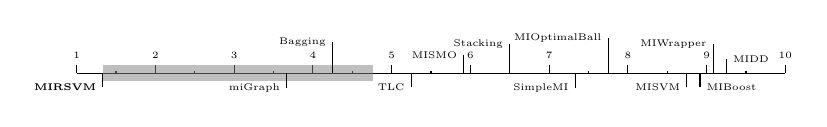
\begin{tikzpicture}
\draw (1,0) -- (10,0);
\foreach \x in {1,2,3,4,5,6,7,8,9,10} {
\draw (\x, 0) -- ++(0,.1) node [above,scale=0.7] {\tiny \x};
\ifthenelse{\x < 10}{\draw (\x+.5, 0) -- ++(0,.03);}{}
}

\coordinate (c0) at (1.3333,0);
\coordinate (c1) at (3.6667,0);
\coordinate (c2) at (8.9167,0);
\coordinate (c3) at (7.75,0);
\coordinate (c4) at (9.25,0);
\coordinate (c5) at (9.0833,0);
\coordinate (c6) at (5.9167,0);
\coordinate (c7) at (8.75,0);
\coordinate (c8) at (7.3333,0);
\coordinate (c9) at (5.25,0);
\coordinate (c10) at (4.25,0);
\coordinate (c11) at (6.5,0);

\node (l0) at (c0) [below left=.05cm and 0cm, align=right,scale=0.7] {\tiny \textbf{MIRSVM}};
\node (l1) at (c1) [below left=.05cm and 0cm, align=right,scale=0.7] {\tiny miGraph};
\node (l2) at (c2) [below right=.05cm and 0cm, align=left,scale=0.7] {\tiny MIBoost};
\node (l3) at (c3) [above left=.3cm and 0cm, align=right,scale=0.7] {\tiny MIOptimalBall};
\node (l4) at (c4) [above right=.05cmand 0cm, align=left,scale=0.7] {\tiny MIDD};
\node (l5) at (c5) [above left=.23cm and 0cm, align=right,scale=0.7] {\tiny MIWrapper};
\node (l6) at (c6) [above left=.1cm and 0cm, align=right,scale=0.7] {\tiny MISMO};
\node (l7) at (c7) [below left=.05cm and 0cm, align=right,scale=0.7] {\tiny MISVM};
\node (l8) at (c8) [below left=.05cm and 0cm, align=right,scale=0.7] {\tiny SimpleMI};
\node (l9) at (c9) [below left=.05cm and 0cm, align=right,scale=0.7] {\tiny TLC};
\node (l10) at (c10) [above left=.25cm and 0cm, align=right,scale=0.7] {\tiny Bagging};
\node (l11) at (c11) [above left=.23cm and 0cm, align=right,scale=0.7] {\tiny Stacking};

\fill[fill=gray,fill opacity=0.5] (1.3333,-0.1) rectangle (4.7683,0.1);

\foreach \x in {0,1,2,3,4,5,6,7,8,9,10,11} {
\draw (l\x) -| (c\x);
};
\end{tikzpicture}}\vspace{-1.3em}
\captionof{figure}{\small Bonferroni-Dunn test for overall ranks comparison}\label{fig:BonfDunnpmeta}
\end{table}
Table~\ref{tab:time} shows the run times, in seconds, for each algorithm. MIRSVM has the fastest run time and is ranked second. MIRSVM shows very good scalability considering the number of features, such as in the webmining dataset which comprises of $5863$ attributes. Additionally, taking into account the number of instances as seen in the two largest datasets, component and function, MIRSVM displays superior scalability. It is important to note that quadratic programming solvers are not the most efficient tools for solving optimization problems in terms of run time, and yet MIRSVM still is shown to perform competitively against the current widely used algorithms. The scalability of MIRSVM is founded on the speedy rate of bag-representative convergence, as shown previously in Figure~\ref{fig:convegence}.

SimpleMI achieves the highest rank and competitive run times because, rather than use the instances in each bag to train a model, it takes the mean value of the instances in a bag and uses that for training. Even though SimpleMI has fast run-times, its performance over the previous metrics has been shown to be random and not as effective as the bag-level methods.

Table~\ref{tab:metarank} shows the ranks achieved by each of the metrics along with the average and meta-ranks, to illustrate the overall performance across all metrics. MIRSVM has the best meta-rank (rank of the ranks) and the miGraph method has the second best. The meta-ranks also highlight the better performance of bag-level methods over instance-level and wrapper methods, emphasizing the importance of training at the bag-level. Not only does MIRSVM use bag-level information during classification, but it also optimizes over the instances within the bag, which helps determine which instances contribute the most information about the bags label. SimpleMI, MIWrapper, MIBoost, MISVM, and MDD have the worst performance compared to MIRSVM and miGraph. Specifically, it is evident from the precision and recall results that MIBoost, MIWrapper, and SimpleMI, for example, classify all bags as negative for datasets that have imbalanced class distributions which favor the negative class. This emphasizes the disadvantage of using wrapper methods and assuming the data distribution of the instances within positive bags. Although these algorithms are popular in literature, the experimental study clearly shows that recent bag-level and ensemble methods easily overcome traditional multi-instance learning algorithms. 

In summary, MIRSVM offers improvement in terms of both accuracy and run-time when compared to referenced methods, especially those utilizing SVM-based algorithms.

\section{Conclusions}
This proposal consisted of a novel formulation and algorithm for the multiple-instance support vector machine problem, which optimizes bag classification via bag-representative selection. First, the primal formulation was posed and its dual was then derived and solution computed using a quadratic programming solver. This formulation was designed to utilize bag-level information and find an optimal separating hyperplane between bags, rather than individual instances, using the standard multi-instance assumption. The SMI assumption states that a bag is labeled positive if and only if at least one instance within a bag is positive, and is negative otherwise. The key features of the proposed algorithm MIRSVM are its ability to identify instances within positive and negative bags, i.e. the support vectors or representatives, that highly impact the decision boundary and margin, as well as avoiding uncertainties and issues caused by techniques that flatten, subset, or under-represent positive instances within positively labeled bags. Additionally, it exhibits desirable convergence and scalability, making it suitable for large-scale learning tasks.

The experimental study showed the better performance of MIRSVM compared with existing multi-instance support vector machines, traditional multi-instance learners, as well as ensemble methods. The results, according to a variety of performance metrics, were compared and further validated using statistical analysis with non-parametric tests which highlight the advantages of using bag-level based and ensemble learners, such as miGraph, Bagging, and Stacking, while showing the instance-level based learners performed poorly in comparison or were deemed as strongly biased and unstable classifiers. Our proposal, MIRSVM, performs statistically better, neither compromising accuracy nor run-time while displaying a robust performance across all of the evaluated datasets. The research outcomes of this chapter have been published in~\cite{melki2018mirsvm}.

\chapter{Novel OnLine SVM using Worst-Violators}\label{chap:ollawv}
Due to the ever-growing nature of dataset sizes, the need for scalable and accurate learning algorithms has become evident. Stochastic gradient descent methods are popular tools used to optimize large-scale learning problems because of their generalizability, simplicity, and scalability. This chapter proposes a novel stochastic, i.e. online, learning algorithm for solving the L1 support vector machine (SVM) problem: \textit{OnLine Learning Algorithm using Worst-Violators} (OLLAWV). This Chapter's scope is concerned with developing a unique algorithm for large data problems without the use of parallelization and distributed techniques. Unlike other stochastic methods, OLLAWV eliminates the need for specifying a maximum number of iterations and the use of a regularization term. Rather than using a regularizer, OLLAWV uses early stopping for controlling the size of the margin. The experimental study, performed under strict nested cross-validation, evaluates and compares the performance of the proposal with $2$ modern SVM kernel methods that have been shown to outperform traditional and widely used approaches for solving L1-SVMs, such as \textit{Sequential Minimal Optimization}. OLLAWV is also compared to $5$ classic non-SVM algorithms. The results over $23$ datasets show OLLAWV's superior performance in terms of accuracy, scalability, and model sparseness, making it suitable for large-scale learning.

\section{Online Learning Background}
Since a comprehensive overview of contemporary online learning algorithms were presented in Chapter~\ref{chap:background}, this section will present the concept of Stochastic (sub)Gradient Descent (SGD) for the unconstrained primal L1-SVM optimization problem, given by Equation~\ref{eqn:reghingeloss}. First, the notation that will be used througout the chapter is introduced, then a brief background on stochastic (sub)gradient descent will be given.

\subsection{Notation}\label{subsec:notation}
\begin{table}[t!]
\small \centering
\caption{Summary of Online Learning Notation}\label{tab:Notation}
\begin{tabularx}{\textwidth}{l@{\extracolsep{\fill}}l}
\hline\noalign{\smallskip}
Definition & Notation\\ 
\noalign{\smallskip}\hline\noalign{\smallskip}
Number of Samples & $n$ \\
Number of Input Attributes & $d$ \\
Input Space & $\bm{X} \in \mathbb{R}^{n \times d}$ \\
Labels & $\bm{Y} \in \{-1,1\}^n$ \\
Sample $i$ & $\bm{x}_i = (x_{i1}, \ldots, x_{id}),\, \forall i \in \set{1,\ldots,n}$ \\
Sample Label $i$ & $y_i \in \set{-1,1},\, \forall i \in \set{1,\ldots,n}$ \\
\noalign{\smallskip}\hline\noalign{\smallskip}
Full Training Dataset & $\mathcal{D} = \{(\bm x_1,y_1), \ldots, \set{\bm x_i,y_i}, \ldots, (\bm x_n,y_n)\}$ \\
\noalign{\smallskip}\hline
\end{tabularx}
\end{table}
Let $\mathcal{D}$ be the full training dataset of $n$ $d$-dimensional samples. Let $\bm{Y} \in \mathcal{D}$ be a vector of $n$ labels corresponding to each sample, such that $\bm{Y} \in \set{-1,1}^n$. In the non-binary (more than two classes) classification cases, $\bm Y \in \ints^n$. Let $\bm{X} \in \mathcal{D}$ be a matrix consisting of $n$ samples that are $d$-dimensional, $\bm{X} \in \mathbb{R}^{n \times d}$. 

\subsection{Stochastic (sub)Gradient Descent}
In the context of large-scale convex learning problems, the advantages of using SGD are its efficiency and simplicity, while maintaining good sample complexity. 

The approach for minimizing a convex, differentiable function $f(\bm{w})$ is an iterative one where the gradient of $f$ is taken at each step and used to update the variable to be minimized. The gradient of function $f : \mathbb{R}^d \rightarrow \mathbb{R}$ at $\bm{w}$, is denoted and defined by $\bigtriangledown f(\bm{w}) = \left(\frac{\partial f(\bm{w})}{\partial w_1}, \ldots, \frac{\partial f(\bm{w})}{\partial w_d}\right)$, the vector of partial derivatives of $f$ with respect to $\bm{w}$. The Gradient Descent (GD) algorithm is as follows: $\bm{w}$ is first initialized to some random value (say $\bm{w}^{(1)} = 0$), and at each iteration, a step is taken in the negative direction of the gradient at that point, as shown in equation~\ref{eqn:gradientupdate},
\begin{equation}
\bm{w}^{(t+1)} \leftarrow \bm{w}^{(t)} - \eta \frac{1}{n} \sum_{i=1}^n\bigtriangledown_w f_i(\bm{w}^{(t)}),
\label{eqn:gradientupdate}
\end{equation}
where $\eta > 0 \in \reals$ is the learning rate and usually decreases with the number of iterations.

After $T$ iterations, the algorithm returns the averaged weight vector $\bm{\bar{w}} = \frac{1}{T}\sum_{t=1}^T \bm{w}^{(t)}$. Different versions of the weight vector could also be returned, such as the last weight vector, $\bm w^T$, or the average of the last 25\% of changes. More information about this can be found in~\cite{Melki2016}. The Gradient Descent algorithm requires that the function being minimized is differentiable. Some loss functions are not differentiable, and in these cases, the subgradient of $f(\bm{w})$ at $\bm{w}^{(t)}$ can be taken instead of the gradient. 

The stochastic gradient descent algorithm is a simplification of that of gradient descent. Rather than computing the gradient of $f$ exactly, at each iteration it is instead an estimation of the gradient on the basis of a single, randomly picked sample $\bm x_i,\, \forall i \in \{1, \ldots, n\}$. The update then becomes,
\begin{equation}
\bm{w}^{(t+1)} \leftarrow \bm{w}^{(t)} - \eta\bigtriangledown_w f_i(\bm{w}^{(t)}).
\label{eqn:gradientupdateo}
\end{equation}
Thus, each iteration of SGD is very cheap in terms of computation since it only deals with the gradient at one sample. Note, the iterative sequence is not determined uniquely by the optimization function, starting point of $\bm w_0$, and sequence of step sizes; rather, it is a stochastic process whose behavior is determined by the sequence of random examples chosen at each iteration~\cite{bottou2010large,bottou2018optimization}.

\subsection{Stochastic Gradient Descent for the Primal L1-SVM Problem}
SVMs were typically treated and solved as a constrained quadratic optimization in dual space. Their early development was hindered because of the quaratic dependence, on the number of samples, of the memory required to efficiently solve them. This lead to the idea of optimizing over subsets of the data, also known as decomposition methods~\cite{boser1992training,Joachims1999,keerthi2001improvements,Platt1998}. Although these methods improved convergence rates, in practice, their superlinear (and sometimes cubic) dependence on the number of samples still was an issue in terms of slow runtimes when learning from massive datasets. Linear SVMs, taking advantage of linear kernels, were shown to outperform decomposition SVMs, motivating research for solving the SVM problem in the primal~\cite{Chapelle2007,panagiotakopoulos2013stochastic}. It has been shown that when finding an approximate solution, primal optimization is superior~\cite{Chapelle2007}. These algorithms for the linear SVM are mostly based on the perceptron~\cite{freund1999large,rosenblatt1958perceptron} - the simplest online, i.e. stochastic, learning algorithm for binary linear classification in the primal space. The perceptron cycles repeatedly, one sample at a time, updating each samples current state in the weight vector, until an appropriate condition is satisfied. By updating cyclically, these types of algorithms are able to process large amounts of data at a much faster speeds with low memory resources, consequently making them suitable for handling large datasets. 

An approach similar to that of the perceptron aims to solve the regularized soft margin loss through stochastic gradient descent, which allows a perceptron-like update while managing the model capacity~\cite{panagiotakopoulos2013stochastic}. This update is the only modification performed by the algorithm when a new sample is given, only occurs if some loss is incurred, and continues to be performed until some user intervention. Due to a lack of meaningful stopping criteria, the algorithm would keep running forever unless some user intervenes. Notable representations of algorithms that use this type of approach can be found in Chapter~\ref{chap:background}. Due to these characteristics, algorithms that use SGD are fundementally different than methods such as mistake-driven perceptron-like approaches. However, Collobert and Bengio later showed that with early stopping, the capacity of the perceptron could be controlled, using the idea of the margin. This was shown in a study comparing perceptrons, multi-layer perceptrons, and SVMs~\cite{collobert2004links}. They also showed that it can be computationally expensive to train SVMs and perceptrons using SGD due to the regularization term, i.e. the term that controls the models capacity, and then showed alternative methods for remedying this issue. Namely, early stopping, and the removal of the regularization term or the learning rate, can control the size of the margin. However, this then raises the question about knowing when it is early enough to stop. This issue, along with the fact that solving the L1-SVM problem in the primal provides a better approximate solution than solving the dual, inspired the investigation for OLLAWV.

\section{OLLAWV: OnLine Learning Algorithm using Worst-Violators}
OLLAWV is an iterative, online learning algorithm for solving the L1-SVM problem using a novel model update procedure while implementing a self-stopping condition. The inspiration behind OLLAWV came from~\cite{kecman2016fast} which presented a generic online learning algorithm tailored not only for SVMs, but also for various other popular classifiers that use different risk functions, with or without a regularization term. The difference, novelty, and advantage of OLLAWV resides in its iterative method, where the weight $\alpha_i$ of the most violating sample i.e., of the \textit{worst-violator}, is only updated in each iteration. A worst violating sample is defined as the sample that has the largest error with respect to the current decision function. Rather than randomly selecting samples to update per iteration, OLLAWV selects (without replacement) the most incorrectly classified sample and updates the model accordingly. By iteratively updating the model using only the worst-violator, the model is essentially finding its support vectors, as well as implicitly defining a stopping criterion. If there are no more violating samples, the algorithm terminates, eliminating the need to define the number of iterations for an algorithm to perform before returning the model, as is the case with most state-of-the-art online algorithms. 

At every iteration, the algorithm selects a worst violating sample that has not been previously chosen, stores its index in vector $\bm S$, and then updates the model. Equation~\ref{eq:wv} shows the method for selecting the worst-violator, where $yo \in \reals$ is the error value, $wv \in \set{1, \ldots, n}$ is the error value's index, $\bm o \in \reals^n$ is the decision function output, and $\neg$ is the `not' symbol. For the L1-SVM, an error value will always be negative which is why the minimum function is used (i.e. the most negative output value or incorrectly classified sample). The worst violating sample becomes the model's support vector because its weight is updated and non-zero. Therefore, OLLAWV's number of iterations is equal to the final model's number of support vectors. This is an interesting property of OLLAWV; if the number of iterations is set beforehand, one is implicitly setting a bound on the number of support vectors. 
\begin{equation}
[yo, wv] = \min \set{y_{wv} \cdot o_{wv}},\, \forall wv \in \set{\neg \bm S}
\label{eq:wv}
\end{equation}

Algorithm~\ref{alg:ollawv} lists OLLAWV's pseudocode and Figure~\ref{fig:ollawv} illustrates the steps taken by OLLAWV. First, the model parameters ($\bm \alpha$, $b$, $\bm S$) and the algorithm variables ($\bm o$, iteration counter ($t$), initial worst-violator index $wv$ and its error $yo$) are first initialized. The worst-violator with respect to the current hyperplane is then found and the model parameters are updated. Once no more violating samples are found or the maximum number of iterations is reached, the model is returned.

OLLAWV performs stochastic gradient descent on the primal L1-SVM objective function given below:
\begin{equation}
\label{eq:l1svm}
\min\limits_{\bm{w} \in \mathcal{H}_o \times \reals} R {\,\,} = {\,\,} \frac{1}{2}||\bm{w}||^2 + C\sum_{i=1}^n \max \set{0, 1 - y_i o_{(w)}(\bm{x}_i)},
\end{equation}
where $o_{(w)}(\bm{x}_i) = \langle\bm w, \bm x_i\rangle$ is a linear predictor, with the bias term excluded for simplicity. Note that the loss function used in Equation~\ref{eq:l1svm} is non-differentiable, but it has a subgradient due to a knick-point at $yo = 1$. The loss function's gradient after the knick-point equals zero, which leads to a sparse model. Hence, when the value of $yo \geq 1$ the loss is zero, and for $yo < 1$ the loss increases linearly. The subgradient of the above cost function is given by:
\begin{equation}
\label{eq:subgrful}
\frac{\partial R}{\partial \bm w} = \begin{cases} 
						\bm w - C \sum_{i=1}^n y_i \bm{x_i} & y_i o_i < 1 \\
						\bm w & \text{otherwise.}
						\end{cases}
\end{equation}
In the stochastic case, the calculation of the gradient needed for the weight update, is \textit{pattern based}, not \textit{epoch based} as in batch gradient descent. It has been shown~\cite{Kecman2001} that the ideal gradient is equal to the sum of the gradients calculated after each sample is presented for fixed weights during the whole epoch. Thus, the stochastic update of $\bm w$ from the subgradient shown in Equation~\ref{eq:subgrful} becomes:
\begin{align*}
\bm w &\leftarrow \bm w - \eta \frac{\partial R}{\partial \bm w} \\
\bm w &\leftarrow \bm w + \eta \begin{cases} 
															C y_i \bm{x_i} - \bm w & y_i o_i < 1 \\
															-\bm w & \text{otherwise},
													 \end{cases}
\end{align*}
where $\eta > 0 \in \reals $ is the learning rate. According to the Representer Theorem, a vector $\bm \alpha \in \reals^n$ exists such that $\bm w = \sum_{i=1}^n \alpha_i \phi(\bm x_i)$ is an optimal solution to Equation~\ref{eq:l1svm}, where $\phi(\cdot)$ is a mapping from feature space to Hilbert space~\cite{Shalev2014}. On the basis of the Representer Theorem, Equation~\ref{eq:l1svm} can be optimized with respect to $\bm \alpha$ instead of $\bm w$. By expressing $\bm w$ this way and mapping input sample $\bm{x_i}$ to $\phi(\bm{x_i})$, the kernelized SGD update becomes:
\begin{equation*}
\centering
\sum_{i=1}^n \alpha_i \phi(\bm x_i) \leftarrow \sum_{i=1}^n \alpha_i \phi(\bm x_i) + \eta \begin{cases} 
															C y_i \phi(\bm{x_i}) - \sum_{i=1}^n \alpha_i \phi(\bm x_i) & y_i o_i < 1 \\[5pt]
															-\sum_{i=1}^n \alpha_i \phi(\bm x_i) & \text{otherwise}.
													 \end{cases}
\end{equation*}
However, OLLAWV optimizes in a stochastic manner, resulting in the following update:
\begin{align*}
&\forall i: \alpha_i \phi(\bm x_i) \leftarrow \alpha_i \phi(\bm x_i) + \eta \begin{cases} 
																													(Cy_i\phi(\bm{x_i}) - \alpha_i \phi(\bm x_i)) & y_i o_i < 1 \\
																													(- \alpha_i \phi(\bm x_i)) & \text{otherwise}
																													 \end{cases} \\							
&\forall i: \alpha_i \leftarrow \alpha_i + \eta \begin{cases} 
																(Cy_i - \alpha_i) & y_i o_i < 1 \\
																(- \alpha_i) & \text{otherwise}.
															\end{cases} 
\end{align*}
The case when the worst violating sample is correctly classified $yo \geq 1$ is OLLAWV's termination condition, i.e. is used as the stopping criterion in the algorithm. Hence the update for $\bm \alpha$ is reduced to the following:
\begin{equation}
\label{eq:alphaupdate}
\forall i: \alpha_i \leftarrow \alpha_i + \eta(Cy_i - \alpha_i)
\end{equation}
If the bias term $b$ is included in Equation~\ref{eq:l1svm}, its stochastic update is as follows:
\begin{equation}
\label{eq:upbias}
\forall i: b \leftarrow b + \eta \frac{C y_i}{n}
\end{equation}
\begin{figure}
\centering
\small
\begin{algorithm}[H]
\caption{OnLine Learning Algorithm using Worst-Violators (OLLAWV)}
\label{alg:ollawv}
\small
\begin{algorithmic}[1]
\renewcommand{\algorithmicrequire}{\textbf{Input:}}
\renewcommand{\algorithmicensure}{\textbf{Output:}}
\Require $\mathcal{D}$, $C$, $\gamma$, $\beta$, $M$
\Ensure  $\bm \alpha$, $b$, $\bm S$
\State $\bm \alpha \leftarrow \bm 0,\, b \leftarrow 0, \bm S \leftarrow \bm 0$ \Comment{Initialize OLLAWV model parameters}
\State $\bm o \leftarrow \bm 0,\, t \leftarrow 0$ \Comment{Initialize the output vector and iteration counter}
\State $wv \leftarrow 0,\, yo \leftarrow y_{wv}*\bm{o}_{wv}$ \Comment{Initialize hinge loss error and worst-violator index}
\While {$yo < M$}
\State $t \leftarrow t + 1$
\State $\eta \leftarrow 2/\sqrt{t}$ \Comment{Learning rate}
\State 
\State $\Lambda \leftarrow \eta*C*y_{wv}$ \Comment{Calculate hinge loss update}
\State $B \leftarrow \left(\Lambda*\beta\right)/n$ \Comment{Calculate bias update}
\State $\bm o \leftarrow \bm o + \Lambda*\mathcal{K}\left(\bm{x}_{\neg \bm S},\, \bm{x}_{wv}, \gamma \right) + B$ \Comment{Update output vector}
\State $\bm \alpha_{wv} \leftarrow \bm \alpha_{wv} + \Lambda$ \Comment{Update worst-violator's alpha value}
\State $b \leftarrow b + B$ \Comment{Update bias term}
\State
\State $\bm S_t \leftarrow wv$ \Comment{Save index of worst-violator}
\State $\left[yo,\, wv\right] \leftarrow \min\limits_{wv \in \set{\neg \bm S}}\set{y_{wv} \cdot o_{wv}}$ \Comment{Find the worst-violator}
\EndWhile 
\end{algorithmic} 
\end{algorithm}
\begin{minipage}{\textwidth}
\small
\adjustbox{scale=0.9}{
\begin{tikzpicture}[%
    node distance=4cm,
    on grid,
    auto
]
\node[block](A) {Initialize training variables};
\node(B)[block, right of=A, text width=6em] {Calculate updates based on worst-violator and current decision boundary};
\draw[arrow] (A) -- (B);
\node(C)[block, right of=B,text width=6.3em] {Update output vector, worst-violator's alpha, \& bias term};
\draw[arrow] (B) -- (C);
\node(D) [decision,right of=C,fill=gray!55,text width=2cm]{while errors exist};
\draw[arrow] (C) -- (D);
\node(E) [block,right of=D]{return $\bm \alpha,\, b, \bm S$};
\draw[arrow] (D) -- node {no} (E);
\draw[arrow] (D.south) --+(0,-0.7cm) -| (B.south) node[below,pos=0.25] {yes} ;
\end{tikzpicture}}
\caption{A summary of the steps performed by OLLAWV. The model parameters ($\bm \alpha$, $b$, $\bm S$) and the algorithm variables ($\bm o$, $t$, $wv$, and $yo$) are first initialized. The worst-violator with respect to the current hyperplane is then found and the model parameters are then updated. Once no more violating samples are found, the model is returned.}
\label{fig:ollawv}
\end{minipage}
\end{figure}

\begin{figure}[t!]
\centering
\begin{minipage}{0.49\textwidth}
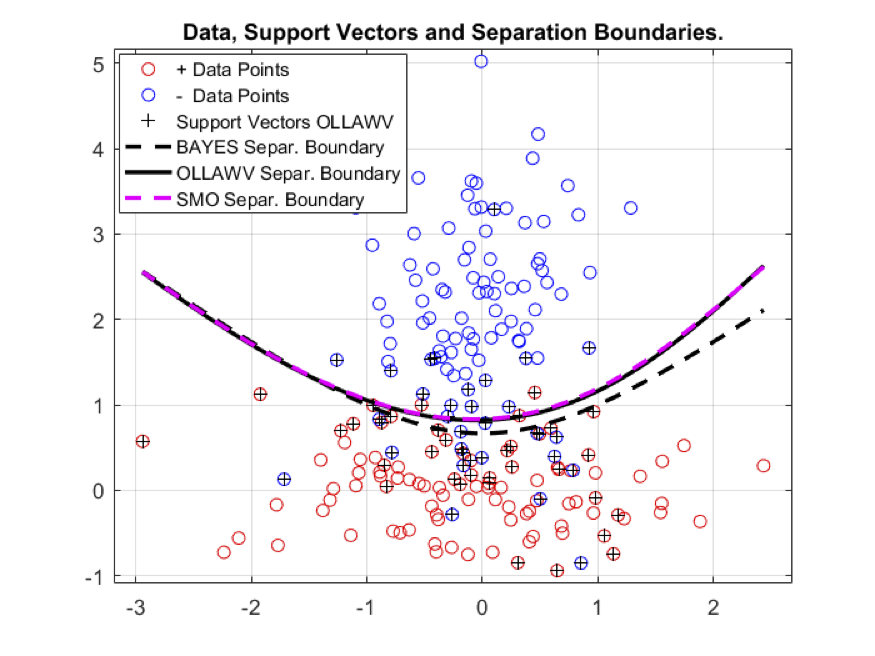
\includegraphics[width=\textwidth]{figures/OLLAWVSeparation.png}
\end{minipage}
\begin{minipage}{0.49\textwidth}
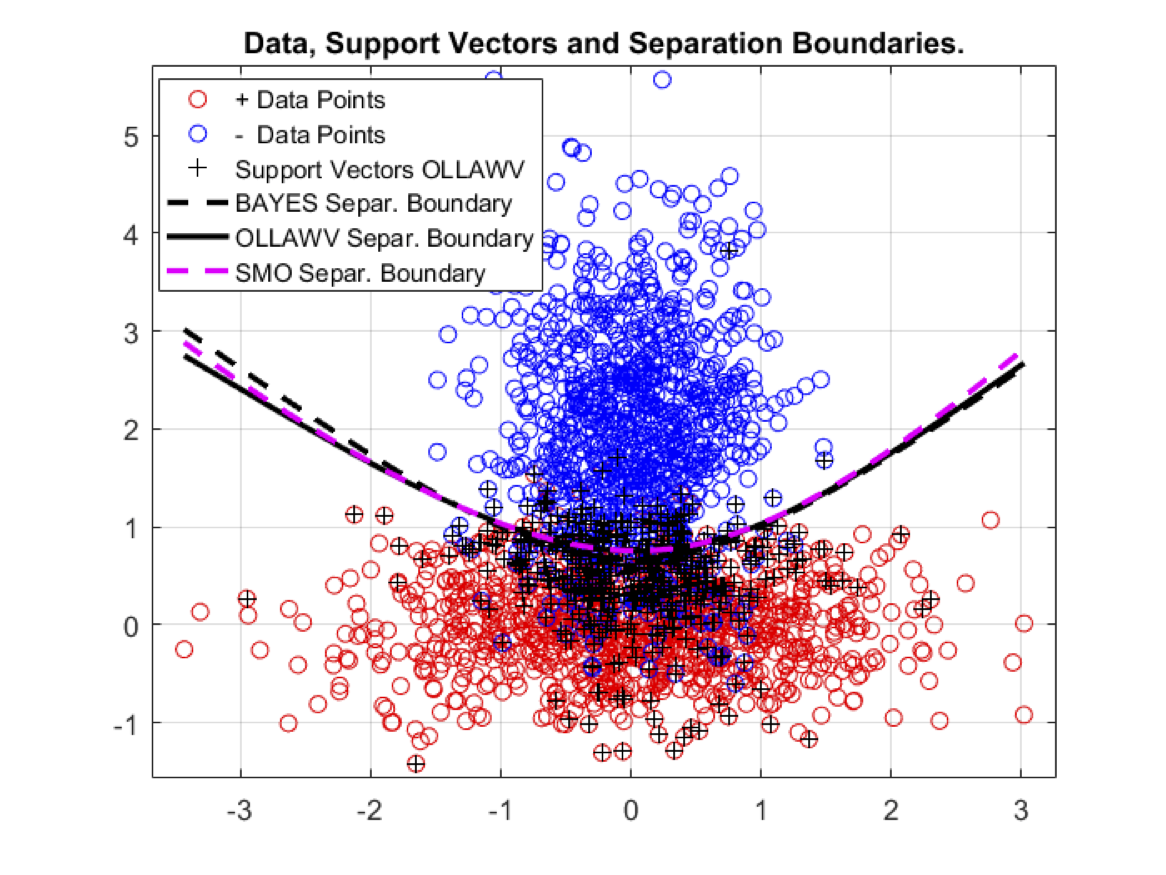
\includegraphics[width=\textwidth]{figures/SeparationOLLAWV2000.png}
\end{minipage}
\caption{A case of classifying 2-dimensional normally distributed data with different covariance matrices, (left) for 200 and (right) 2000 data points. The theoretical separation boundary (denoted as the Bayes Separation Boundary) is quadratic and is shown as the dashed black curve. The other two separation boundaries shown are the ones obtained by OLLAWV and SMO (implemented within LIBSVM), respectively. In this particular case (left), the difference between the OLLAWV boundary and the SMO boundary is hardly visible. The case presented on the right shows that, with an increase of training samples, the OLLAWV and SMO boundaries converge to the theoretical Bayesian solution.}
\label{fig:ollawvseparation}
\end{figure}

In this experimental study, $\eta = 2/\sqrt{t}$ is used, where $t$ is the current iteration; however, other learning rates such as $\eta = 1/t$ can also be used. Let $\Lambda = \eta Cy_i$ and $\Rho = \eta \alpha_i$ be the update parameters for OLLAWV, and the $\bm \alpha$ update can be expressed as: $\alpha_i \leftarrow \alpha_i + (\Lambda - \Rho)$. Note that $\Lambda$ is the update resulting from the loss function and $\Rho$ is derived from the regularizer term in Equation~\ref{eq:l1svm}. In the case of OLLAWV, $\Rho = 0$ because samples are never updated more than once and their initial $\alpha$ value is always $0$. It is important to note that in OLLAWV's case, $\Lambda$ never equals $0$ because the samples being updated are worst-violators, meaning they are misclassified or incur some loss. The values of the decision function (output vector $\bm o \in \reals^n$ in Algorithm~\ref{alg:ollawv}), from which a worst-violator is found, changes per iteration based on the influence of the support-vectors that have been previously updated. From Equation~\ref{eq:output}, the output vector update becomes the following: 
\begin{equation}
\label{eq:upoutput}
\bm o \leftarrow \bm o + \Lambda*\mathcal{K}\left(\bm{x}_{\neg \bm S},\, \bm{x}_{wv}, \gamma \right) + B
\end{equation}
where $\mathcal{K}(\cdot)$ is the Gaussian radial basis function (RBF) kernel, $\gamma \in \reals$ is its parameter, and $B = (\Lambda * \beta)/n$ denotes the bias update. Only non-support vector output values are calculated per iteration, as denoted by $\bm x_{\neg \bm S}$ in the kernel function, because samples are never selected to be updated more than once. Because the output values scale with the $C$ value, the stopping criteria for OLLAWV is also set to scale with $C$, rather than the classic formulation $y_i o_i \geq 1$. If the value of $C$ is very large, $y_i o_i$ will never be greater than 1 and the algorithm will never terminate. Therefore, the stopping criteria is set to be $y_i o_i \geq M$, where $M \in \reals$ is a scaled value of $C$. For the $B$ calculation in Equation~\ref{eq:upoutput}, $\beta \in \set{0,1}$ indicates whether the bias term is to be used. If $b$ is not a part of the model, it should be omitted from Equations~\ref{eq:output} and~\ref{eq:upoutput} by setting $\beta = 0$, otherwise $\beta = 1$. 

OLLAWV is a stochastic gradient method (SGM) that has a convex cost function. Its learning rate coefficient can decrease linearly or semi-linearly during the learning stage. Hence, OLLAWV shares the complexity characteristics of SGM methods. Primarily, it can achieve linear convergence, making it a particularly convenient and practical method for solving very large machine learning problems. OLLAWV also works over a cost function without local minima, always leading towards the global minimum, even though it stops the learning process as soon as all samples are outside the prescribed margin. Figure~\ref{fig:ollawvseparation} shows the decision boundaries achieved by OLLAWV versus SMO (implemented within LIBSVM) and Bayes for toy datasets. 

\section{Experimental Environment, Results, and Analysis}\label{sec:exp}
This section presents two experimental setups of our contribution against other state-of-the-art algorithms on $23$ different benchmark datasets. The first study, presented in Section~\ref{subsec:expsvm}, compares OLLAWV to two other SVM kernel methods, and the second compares OLLAWV to $5$ non-SVM methods, shown in Section~\ref{subsec:nonsvmexp}. In each section, the experimental setups are first described and the state-of-the-art methods are listed. The results and statistical analysis are then presented and analyzed. The main aim of the experiments is to compare our contribution to other support vector machine solvers that have been shown to surpass popular and widely used SVM kernel methods in terms of memory consumption, runtime, and accuracy. The supplemental experimental study in~\ref{subsec:nonsvmexp} was conducted to emphasize the better performance of OLLAWV against non-SVM algorithms.
\begin{table}[t!]
\caption{Classification Datasets}
\footnotesize
\centering
\label{tab:ollawvDataset}
\begin{tabularx}{0.7\textwidth}{l@{\extracolsep{\fill}}rrr}
\hline\noalign{\smallskip}
Dataset & \# Samples & \# Attributes & \# Classes \\
\noalign{\smallskip}\hline\noalign{\smallskip}
\textbf{\textit{small datasets}} & \\
iris & 150 & 4 &  3  \\ 
teach & 151 & 5 &  3  \\ 
wine & 178 & 13 &  3  \\ 
cancer & 198 & 32 &  2  \\ 
sonar & 208 & 60 &  2  \\ 
glass & 214 & 9 &  6  \\ 
vote & 232 & 16 &  2  \\ 
heart & 270 & 13 &  2  \\ 
dermatology & 366 & 33 &  6  \\ 
prokaryotic & 997 & 20 &  3  \\ 
eukaryotic & 2,427 & 20 &  4  \\ 
\textbf{\textit{medium datasets}} & \\
optdigits & 5,620 & 64 &  10  \\ 
satimage & 6,435 & 36 &  6  \\ 
usps & 9,298 & 256 &  10  \\ 
pendigits & 10,992 & 16 &  10  \\ 
reuters & 11,069 & 8,315 &  2  \\ 
letter & 20,000 & 16 &  26  \\ 
\textbf{\textit{large datasets}} & \\
adult & 48,842 & 123 &  2  \\ 
w3a & 49,749 & 300 &  2  \\ 
shuttle & 58,000 & 7 &  7  \\ 
web (w8a) & 64,700 & 300 &  2  \\ 
ijcnn1 & 141,691 & 22 &  2  \\ 
intrusion & 5,209,460 & 127 &  2  \\  
\noalign{\smallskip}\hline
\end{tabularx}
\end{table}

Table~\ref{tab:ollawvDataset} presents a summary of the $23$ datasets used throughout the experiments, where the number of attributes (dimensionality), classes, and samples are shown. The datasets used and the results obtained are divided into three groups: \textit{small}, \textit{medium} and \textit{large}. The datasets were obtained from the UCI Machine Learning repository\footnote{\url{http://archive.ics.uci.edu/ml/index.php}}, and the LIBSVM\footnote{\url{https://www.csie.ntu.edu.tw/~cjlin/libsvmtools/datasets/}}, and the LibCVM\footnote{\url{http://c2inet.sce.ntu.edu.sg/ivor/cvm.html}} sites~\cite{Lichman:2013,CC01a,tsang2005core}. 

\subsection{SVM Experimental Setup}\label{subsec:expsvm}
The experimental setup was designed to evaluate differences in performance of the proposed OLLAWV method against the state-of-the-art algorithms: \textit{Minimal Norm SVM} (MNSVM) \cite{strack2013geometric} and \textit{Non-Negative Iterative Single Data Algorithm} (NNISDA)~\cite{zigic2016}. These algorithms were chosen because they have shown considerable performance in runtime, memory consumption, and accuracy against the popular and widely used LIBSVM and LibCVM pagackes. In~\cite{strack2013geometric}, it was shown that MNSVM outperforms both the L1 and L2 implementations of LIBSVM, and BVM embedded in LibCVM. NNISDA was then compared to MNSVM in~\cite{zigic2016}, and showed an added improvement in runtime performance. MNSVM was implemented in an open source C++ framework called ``GSVM \textendash ~Command Line Tool for Geometric SVM Training\footnote{\url{https://github.com/strackr/gsvm}}''. Both, NNISDA and OLLAWV were implemented as additional modules within Strack-Kecman's code, keeping the experimental environment controlled for all three algorithms. The experiments for all methods were run on the same machine containing two Intel Xeon X5680 CPUs (6-core, 3.33 GHz) and 96 GB of RAM.

Experiments were performed using double, or nested, $5$-fold cross-validation in order to objectively evaluate the models' performances and tune hyper-parameters. In the outer loop, the data are separated into $5$ equally sized folds and each part is held out in turn as the test set, and the remaining four parts are used as the training set. In the inner loop, $5$-fold cross-validation is also used over the training set assigned by the outer loop, where the best hyper-parameters are chosen. The best model obtained by the inner loop is then applied on the outer loop's test set. This procedure ensures the model's performance is not optimistically biased as when using a single loop of $k$-fold cross-validation. It ensures the class labels of the test data will not be seen when tuning the hyper-parameters, which is consistent with real-world applications. Obviously, such a rigorous procedure is computationally expensive, but the goal is to fairly compare different classification models on the same data sets, with the same cross-validation procedure, and hyper-parameters. First, the datasets were normalized by linear transformation of the feature values to the range $[0,1]$. Then, the training process, also involving model selection using pattern search, was performed. The best hyper-parameters were chosen from the following $8 \times 8$ possible combinations, shown in Equations~\eqref{eq:paramColla} and~\eqref{eq:paramGolla}, and were also used for the competing SVM methods.
\begin{subequations}
\label{eq:hyperparamolla}
\begin{align}
C \in \set{4^n}, & \,\,\,\,\,n = \set{-2, \ldots, 5} \label{eq:paramColla}\\
\gamma \in \set{4^n},  & \,\,\,\,\,n = \set{-5, \ldots, 2} \label{eq:paramGolla}
\end{align}
\end{subequations}
The $\gamma$ parameter refers to that of the Gaussian RBF kernel, given by:
\begin{equation}
\label{eq:rbf}
\mathcal{K}(\bm{x_i},\bm{x_j}) = e^{-\gamma\norm{\bm{x_i} - \bm{x_j}}^2}.
\end{equation}

To deal with multi-class classification problems, the one-vs-one, or pairwise, approach was used. The pairwise training procedure trains $c(c - 1)/2$ binary classifiers, a classifier for each possible pair of classes, where $c$ is the number of classes. During the prediction phase, a voting scheme is used where all $c(c - 1)/2$ models predict an unseen data sample and the class that received the highest number of votes is considered to be the sample’s true class.

\begin{table}[t!]
\centering
\caption{Comparison of OLLAWV vs. NNISDA and MNSVM}
\scriptsize
\label{tab:results}
\resizebox{\textwidth}{!}{\begin{tabularx}{1.1\textwidth}{l@{\extracolsep{\fill}}cccrrrccc}
\noalign{\smallskip}\hline\noalign{\smallskip}
\multicolumn{1}{l}{Dataset} & \multicolumn{3}{c}{Accuracy (\%)} & \multicolumn{3}{c}{Runtime (s)} & \multicolumn{3}{c}{Support Vectors (\%)} \\
\cmidrule(lr){2-4}
\cmidrule(lr){5-7}
\cmidrule(lr){8-10} 
 & OLLAWV & NNISDA & MNSVM & OLLAWV & NNISDA & MNSVM & OLLAWV & NNISDA & MNSVM \\
\noalign{\smallskip}\hline\noalign{\smallskip}
\textbf{\textit{small datasets}} & & & & & & & & & \\
iris & \textbf{97.33} & 94.00 & 96.67 & \textbf{0.05} & 0.27 & 3.57 & \textbf{13.50} & 40.20 & 29.80 \\
teach & 52.32 & 52.31 & \textbf{52.95} & \textbf{0.12} & 0.44 & 8.85 & \textbf{69.19} & 99.80 & 87.40 \\
wine & \textbf{98.87} & 96.60 & 96.60 & \textbf{0.28} & 0.43 & 4.84 & \textbf{15.02} & 44.40 & 48.60 \\
cancer & 80.36 & \textbf{81.86} & 81.38 & \textbf{0.49} & 0.85 & 4.46 & \textbf{42.79} & 83.80 & 89.60 \\
sonar & \textbf{92.32} & 89.48 & 87.57 & \textbf{0.59} & 0.98 & 3.03 & \textbf{31.26} & 73.00 & 66.00 \\
glass & \textbf{72.41} & 67.81 & 69.30 & \textbf{0.46} & 1.01 & 11.94 & \textbf{62.84} & 90.80 & 87.60 \\
vote & \textbf{96.54} & 96.11 & 93.99 & \textbf{0.26} & 0.46 & 1.49 & \textbf{13.36} & 33.20 & 34.00 \\
heart & 82.22 & \textbf{83.33} & \textbf{83.33} & \textbf{0.50} & 0.91 & 6.45 & \textbf{37.69} & 73.00 & 82.00 \\
dermatology & 97.82 & \textbf{98.36} & \textbf{98.36} & \textbf{1.62} & 2.47 & 11.68 & \textbf{36.94} & 59.00 & 59.80 \\
prokaryotic & 88.96 & 88.86 & \textbf{88.97} & \textbf{6.09} & 10.64 & 50.86 & \textbf{29.01} & 51.20 & 49.00 \\
eukaryotic & 77.38 & 79.56 & \textbf{81.21} & 61.95 & \textbf{49.16} & 342.76 & \textbf{54.11} & 76.40 & 72.60 \\
\textbf{\textit{medium datasets}} & & & & & & & & & \\
optdigits & 99.11 & 99.29 & \textbf{99.31} & \textbf{411} & 528 & 787 & \textbf{28.64} & 31.60 & 30.60 \\
satimage & 91.66 & \textbf{92.39} & 92.35 & 1,334 & \textbf{687} & 1,094 & \textbf{20.72} & 45.00 & 44.80 \\
usps & 97.49 & 98.05 & \textbf{98.24} & 10,214 & \textbf{5,245} & 7,777 & \textbf{11.22} & 29.40 & 28.00 \\
pendigits & 99.56 & \textbf{99.62} & 99.61 & \textbf{723} & 909 & 1,500 & \textbf{10.27} & 17.60 & 16.60 \\
reuters & 98.03 & \textbf{98.08} & 97.99 & \textbf{954} & 1,368 & 1,657 & \textbf{8.770} & 18.20 & 18.60 \\
letter & 96.99 & 99.11 & \textbf{99.13} & \textbf{5,259} & 12,009 & 26,551 & \textbf{43.56} & 57.60 & 56.60 \\
\textbf{\textit{large datasets}} & & & & & & & & & \\
adult & 84.75 & 85.07 & \textbf{85.13} & \textbf{21,025} & 72,552 & 123,067 & \textbf{34.66} & 56.00 & 56.60 \\
w3a & \textbf{98.86} & 98.82 & 98.82 & \textbf{6,532} & 15,951 & 24,562 & \textbf{3.270} & 14.60 & 12.40 \\
shuttle & 99.77 & 99.83 & \textbf{99.87} & \textbf{2,833} & 7,420 & 45,062 & \textbf{2.010} & 6.00 & 16.40 \\
web & 98.94 & \textbf{99.00} & 99.00 & \textbf{12,067} & 30,583 & 38,040 & \textbf{4.320} & 13.20 & 10.80 \\
ijcnn1 & 98.31 & 99.34 & \textbf{99.41} & \textbf{162,587} & 296,917 & 370,144 & 16.36 & 11.00 & \textbf{7.600} \\
intrusion & \textbf{99.77} & 99.67 & 99.66 & \textbf{2,402,804} & 4,646,810 & 3,772,113 & \textbf{0.780} & 2.000 & 1.700 \\
\noalign{\smallskip}\hline\noalign{\smallskip}
Average & \textbf{91.29} & 91.15 & 91.25 & \textbf{114,209} & 221,350 & 191,861 & \textbf{25.66} & 44.65 & 43.79 \\
Ranks & \textbf{1.739} & 2.022 & 2.239 & \textbf{1.217} & 1.913 & 2.869 & \textbf{1.087} & 2.609 & 2.304 \\
\noalign{\smallskip}\hline\noalign{\smallskip}
\end{tabularx}}
\\ \vspace{1em}
\begin{minipage}{0.3\textwidth}
\centering
\resizebox{0.9\textwidth}{!}{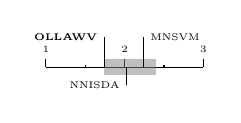
\begin{tikzpicture}
\draw (1,0) -- (3,0);
\foreach \x in {1,2,3} {
\draw (\x, 0) -- ++(0,.1) node [above,scale=0.7] {\tiny \x};
\ifthenelse{\x < 3}{\draw (\x+.5, 0) -- ++(0,.03);}{}
}

\coordinate (c0) at (1.7391,0);
\coordinate (c1) at (2.0217,0);
\coordinate (c2) at (2.2391,0);

\node (l0) at (c0) [above left=.25cm and 0cm, align=right,scale=0.7] {\tiny \textbf{OLLAWV}};
\node (l1) at (c1) [below left=.1cm and 0cm, align=right,scale=0.7] {\tiny NNISDA};
\node (l2) at (c2) [above right=.25cm and 0cm, align=right,scale=0.7] {\tiny MNSVM};

\fill[fill=gray,fill opacity=0.5] (1.7391,-0.1) rectangle (2.3991,0.1);

\foreach \x in {0,1,2} {
\draw (l\x) -| (c\x);
};
\end{tikzpicture}}
\captionsetup{width=0.95\linewidth}
\captionof{figure}{\small Bonferroni-Dunn test for Accuracy}\label{fig:BonfDunnaccolla}
\end{minipage}
\hspace{0.5em}
\begin{minipage}{0.3\textwidth}
\centering
\resizebox{0.8\textwidth}{!}{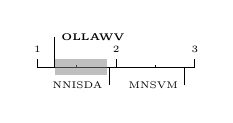
\begin{tikzpicture}
\draw (1,0) -- (3,0);
\foreach \x in {1,2,3}{
\draw (\x, 0) -- ++(0,.1) node [above,scale=0.7] {\tiny \x};
\ifthenelse{\x < 3}{\draw (\x+.5, 0) -- ++(0,.03);}{}
}

\coordinate (c0) at (1.2174,0);
\coordinate (c1) at (1.913,0);
\coordinate (c2) at (2.8696,0);

\node (l0) at (c0) [above right=.25cm and 0cm, align=right,scale=0.7] {\tiny \textbf{OLLAWV}};
\node (l1) at (c1) [below left=.1cm and 0cm, align=right,scale=0.7] {\tiny NNISDA};
\node (l2) at (c2) [below left=.1cm and 0cm, align=right,scale=0.7] {\tiny MNSVM};

\fill[fill=gray,fill opacity=0.5] (1.2174,-0.1) rectangle (1.8774,0.1);

\foreach \x in {0,1,2} {
\draw (l\x) -| (c\x);
};
\end{tikzpicture}}
\captionsetup{width=0.8\linewidth}
\captionof{figure}{\small Bonferroni-Dunn test for Runtime}\label{fig:BonfDunncpu}
\end{minipage}
\hspace{0.5em}
\begin{minipage}{0.3\textwidth}
\centering
\resizebox{0.8\textwidth}{!}{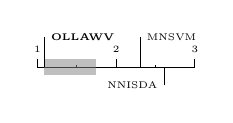
\begin{tikzpicture}
\draw (1,0) -- (3,0);
\foreach \x in {1,2,3} {
\draw (\x, 0) -- ++(0,.1) node [above,scale=0.7] {\tiny \x};
\ifthenelse{\x < 3}{\draw (\x+.5, 0) -- ++(0,.03);}{}
}

\coordinate (c0) at (1.087,0);
\coordinate (c1) at (2.6087,0);
\coordinate (c2) at (2.3043,0);

\node (l0) at (c0) [above right=.25cm and 0cm, align=right,scale=0.7] {\tiny \textbf{OLLAWV}};
\node (l1) at (c1) [below left=.1cm and 0cm, align=right,scale=0.7] {\tiny NNISDA};
\node (l2) at (c2) [above right=.25cm and 0cm, align=right,scale=0.7] {\tiny MNSVM};

\fill[fill=gray,fill opacity=0.5] (1.087,-0.1) rectangle (1.747,0.1);

\foreach \x in {0,1,2} {
\draw (l\x) -| (c\x);
};
\end{tikzpicture}}
\captionsetup{width=0.95\linewidth}
\captionof{figure}{\small Bonferroni-Dunn test for \% Support Vectors}\label{fig:BonfDunnsv}
\end{minipage}
\end{table}

\subsection{SVM Comparison Results and Statistical Analysis}\label{subsec:ollawvresults}
The classification performance was measured using the following metrics: accuracy, runtime, and the percentage of support vectors (size of the model). Table~\ref{tab:results} displays the results for OLLAWV and the two state-of-the-art methods. The percentage of support vectors was reported for analyzing the complexities of the resulting models over the variously sized datasets. In order to analyze the performances of the multiple models, non-parametric statistical tests are used to validate the experimental results obtained~\cite{Derrac2011}. The Iman-Davenport non-parametric test is run to investigate whether significant differences exist among the performance of the algorithms by ranking them over the datasets used, using the Friedman test. The algorithm ranks for each metric are presented in the last row of Table~\ref{tab:results}, and the lowest (best) rank value is typeset in bold. After the Iman-Davenport test indicates significant differences (with $p$-value =  $0.2397$ for accuracy, and $p$-value =  $0$ for runtime and percent support vectors), the Bonferroni-Dunn post-hoc test is then used to find where they occur between algorithms by assuming the classifiers' performances are different by at least some critical value (critical distance is $0.66$ for $\alpha = 0.05$). Below Table~\ref{tab:results}, Figures~\ref{fig:BonfDunnaccolla}, \ref{fig:BonfDunncpu}, and \ref{fig:BonfDunnsv} highlight the critical distance (in gray) from the best ranking algorithm to the rest. The algorithms to the right of the critical distance bar perform statistically significantly worse than the control algorithm, OLLAWV.
% small data speedup [1.0720    6.2136]
% medium data speed [2.3860    4.5274]
% large data speedup [2.06-NNISDA 2.93-MNSVM]
\begin{figure}[t!]
\centering
\begin{minipage}{0.49\textwidth}
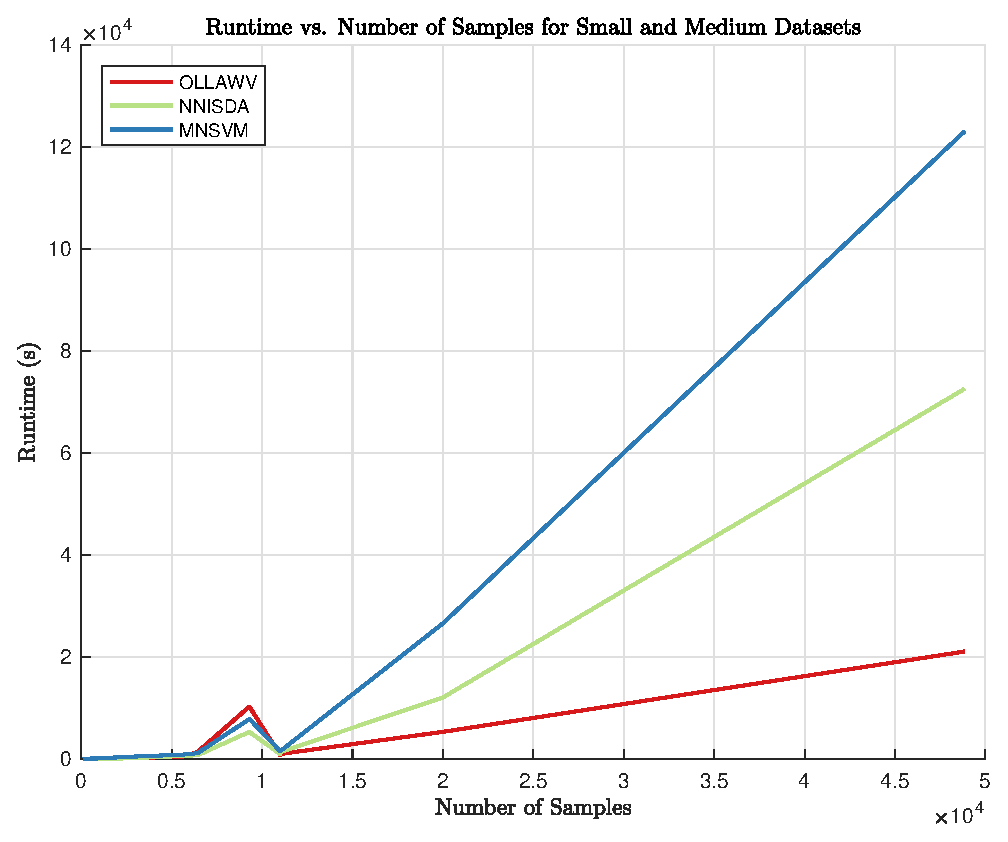
\includegraphics[width=\textwidth]{figures/CPU_vs_NumData_SM.eps}
\end{minipage}
\begin{minipage}{0.49\textwidth}
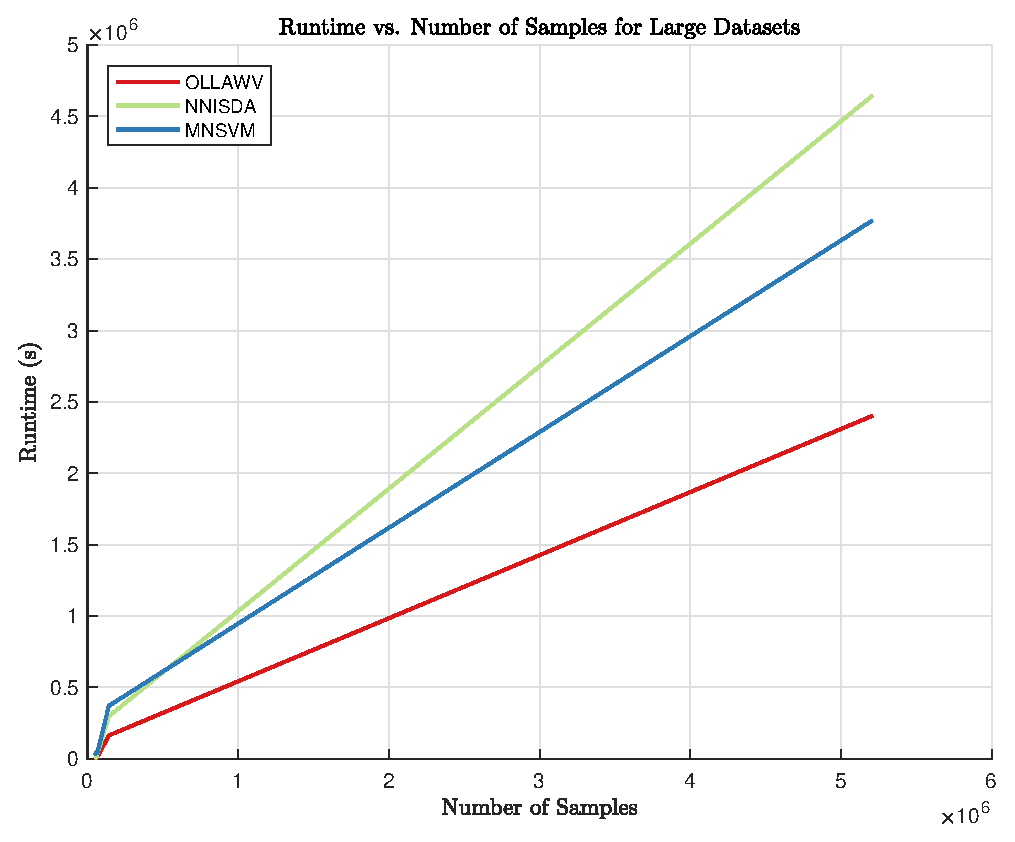
\includegraphics[width=\textwidth]{figures/CPU_vs_NumData_L.eps}
\end{minipage}
\caption{\small Runtime in seconds versus the number of samples, divided into two groups: small \& medium (left) versus large (right). Note OLLAWV's gradual increase in runtime as the number of samples increases compared to NNISDA and MNSVM's steeper change. In almost all cases, OLLAWV displays superior runtime over state-of-the-art. Runtime depends upon many characteristics: dimensionality, class-overlapping, complexity of the separation boundary, number of classes as well as upon the number of support vectors, which partly explains the tiny bump in the left figure. }
\label{fig:cpuvssamples}
\end{figure}

The results in Table~\ref{tab:results} indicate that OLLAWV outperforms NNISDA and MNSVM in terms of accuracy, runtime, and model complexity. Although the differences in accuracy between the methods is not very large, on average, OLLAWV is about $2$ times faster than NNISDA and MNSVM. As mentioned previously, OLLAWV aims to speed up the learning process without sacrificing the model's accuracy. This stems from OLLAWV's ability to produce sparse models, as is shown by the averaged percentage of support vectors. The speedup that OLLAWV presents is proportional to the model complexity and the experimental results show that OLLAWV produces, on average, models that are $1.7$ times smaller than the two state-of-the-art methods used. This highlights the applicability and advantage that OLLAWV has for learning from large datasets. 

\begin{figure}[t!]
\centering
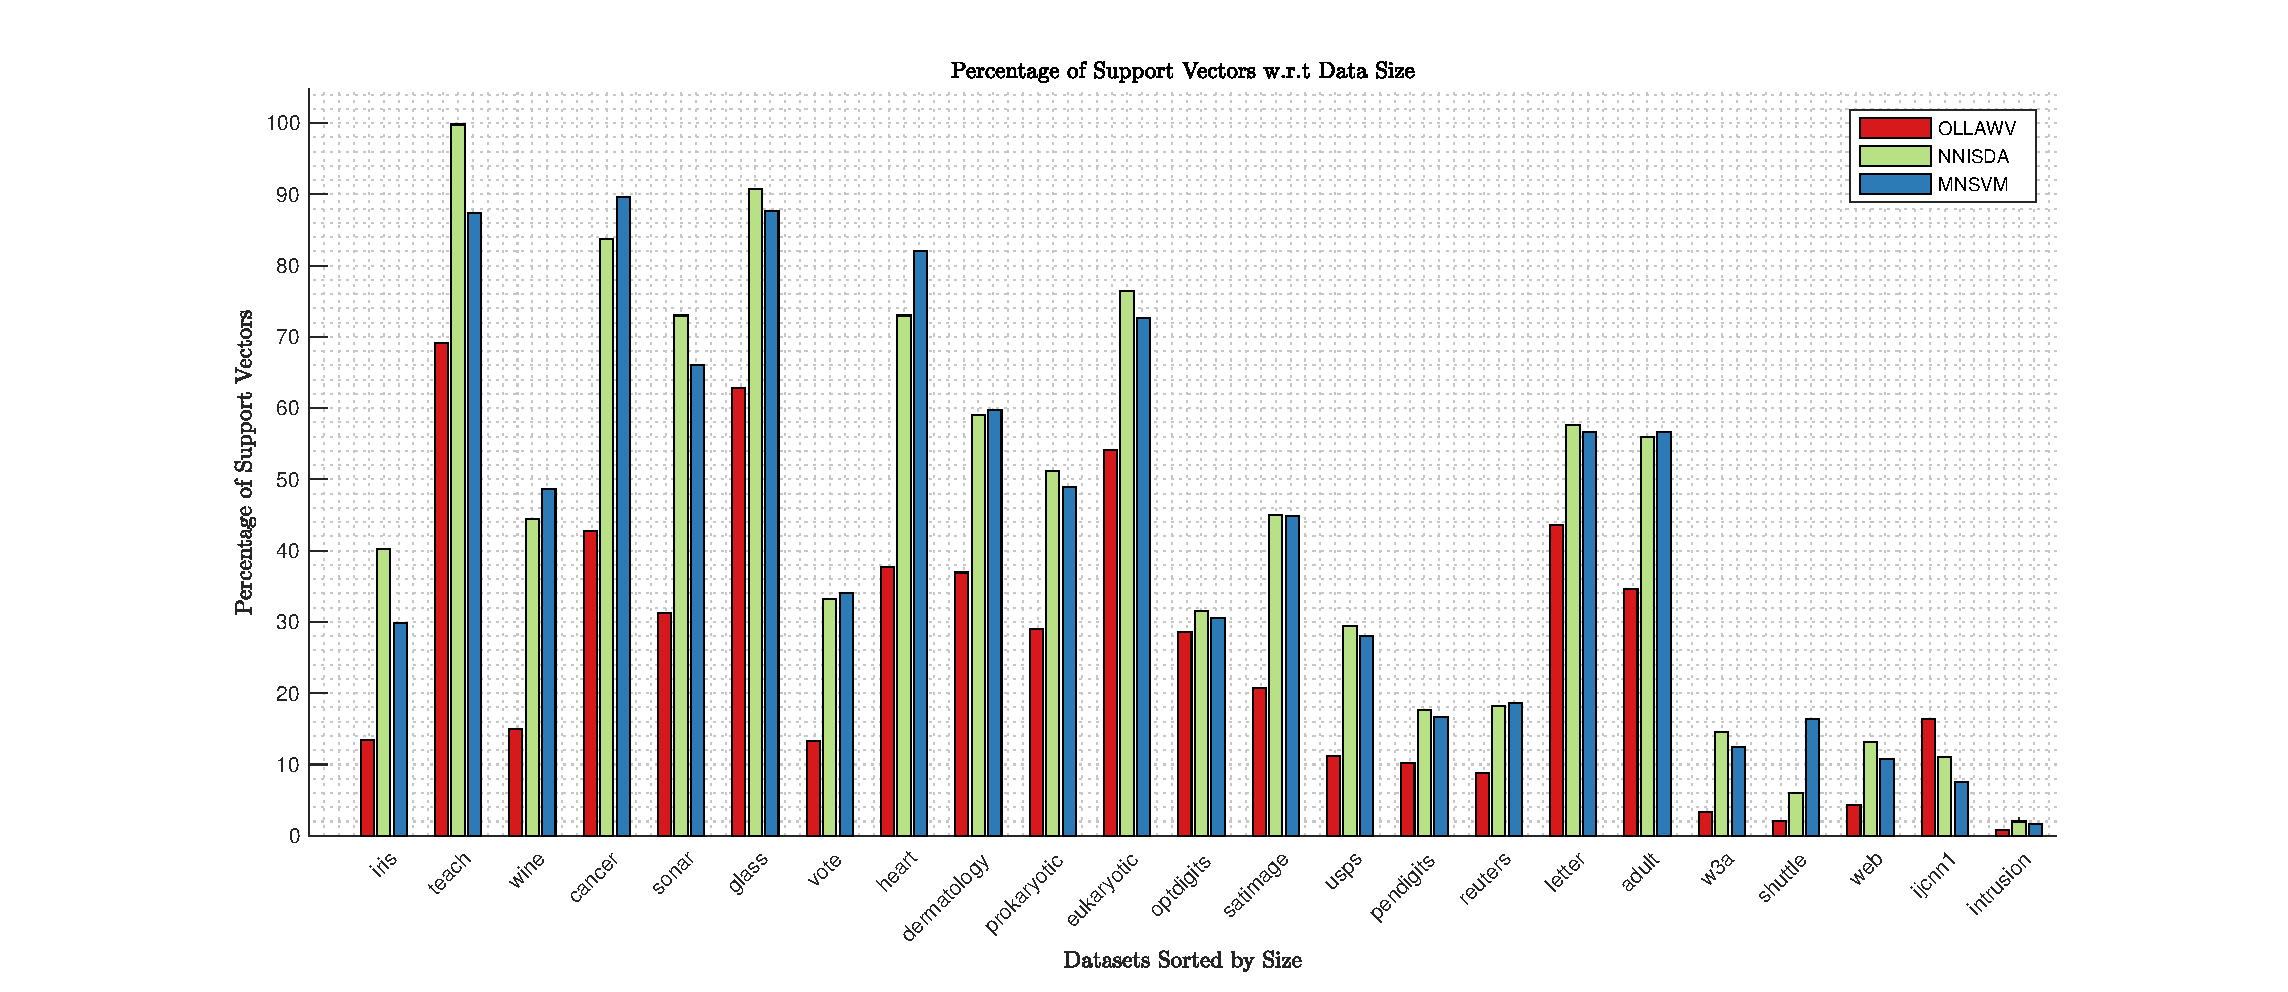
\includegraphics[trim={3.2cm 0 3.2cm 0},clip,width=\textwidth]{figures/PSV_vs_NumData.eps}
\caption{Size of the model given as percentage of support vectors with respect to the number of samples  versus the number of samples. Note that OLLAWV’s percentage of support vectors is always smaller (except in one case) than NNISDA's and MNSVM's ones.}
\label{fig:psvvssamples}
\end{figure}
Figures~\ref{fig:BonfDunnacc}, \ref{fig:BonfDunncpu}, and \ref{fig:BonfDunnsv} show the results of the statistical analysis for accuracy, runtime, and percentage of support vectors. Figures~\ref{fig:BonfDunncpu} and~\ref{fig:BonfDunnsv} show that OLLAWV is statistically significantly better than MNSVM and NNISDA for runtime and percentage of support vectors (model size). At the same time, Figure~\ref{fig:BonfDunnacc} emphasizes what was mentioned earlier: OLLAWV is shown to speed up the learning process without sacrificing model accuracy against the state-of-the-art methods used. 

Figure~\ref{fig:cpuvssamples} plots the correlation of OLLAWV, NNISDA, and MNSVM's runtime versus number of samples for the small, medium, and large datasets. The figure clearly emphasizes the benefit of using OLLAWV for large-scale learning due to its gradual increase in runtime as the number of samples increases in comparison to NNISDA and MNSVM. Figure~\ref{fig:psvvssamples} shows the correlation between OLLAWV, NNISDA, and MNSVM's percentage of support vectors and the number of samples for all datasets. It highlights OLLAWV's model sparseness in comparison to the competing methods, while mirroring the runtime results. 

\subsection{Non-SVM Experimental Setup}\label{subsec:nonsvmexp}
The supplemental experimental setup was designed to compare the performance of the proposed OLLAWV against the following $5$ popular and widely-used non-SVM algorithms: \textit{k-Nearest Neighbors ($k$-NN)}, \textit{J48}, \textit{JRip}, \textit{Na\"ive Bayes}, and \textit{Logistic}. These methods have been implemented within the Weka framework~\cite{eibe2016weka}. The experiments were performed under the same nested $5$-fold cross-validation framework as the SVM algorithm experimental study which was described in Section~\ref{subsec:expsvm}. The following hyper-parameters shown in Table~\ref{tab:hyp} were used for the non-SVM algorithms.

\begin{table}[H]
\small
\caption{Non-SVM Algorithm Hyper-parameters}
\label{tab:hyp}
\centering
\begin{tabularx}{\textwidth}{l@{\extracolsep{\fill}}l}
\noalign{\smallskip}\hline\noalign{\smallskip}
Algorithm & Parameters \\
\noalign{\smallskip}\hline\noalign{\smallskip}
$k$-NN &  Number of neighbors: $k \in \set{1,\, 3,\, 5,\, 7}$\\
J48 & Pruning: $\set{\text{True},\, \text{False}}$, Pruning Confidence: $\set{0.1,\,0.25,\,0.5}$\\
JRip & Pruning: $\set{\text{True},\, \text{False}}$  \\
Naive Bayes & Use kernel estimation: $\set{\text{True},\, \text{False}}$  \\
Logistic & Log-likelihood: $\set{1\text{e}^{-7},\, 1\text{e}^{-8},\,1\text{e}^{-9}}$  \\
\noalign{\smallskip}\hline\noalign{\smallskip}
\end{tabularx}
\end{table}

\subsection{Non-SVM Results and Statistical Analysis}
%CD for alpha = 0.05 is 1.3911990032582209
\begin{table}[t!]
\caption{Accuracy (\%) Comparison for Non-SVM Methods vs. OLLAWV}
\scriptsize
\centering
\label{tab:OtherResultsacc}
\begin{tabularx}{\textwidth}{l@{\extracolsep{\fill}}cccccc}
\noalign{\smallskip}\hline\noalign{\smallskip}
Dataset & OLLAWV & $k$-NN & J48 & JRip & Na\"ive Bayes & Logistic \\
\noalign{\smallskip}\hline\noalign{\smallskip}
\textbf{\textit{small datasets}} & & & & & & \\
iris & \textbf{97.33 $\pm$ 1.49} & 96.00 $\pm$ 3.65 & 94.00 $\pm$ 2.79 & 90.67 $\pm$ 4.35 & 96.00 $\pm$ 2.79 & 97.33 $\pm$ 2.79  \\
teach & 52.32 $\pm$ 3.46 & \textbf{59.64 $\pm$ 2.89} & 49.72 $\pm$ 7.58 & 56.75 $\pm$ 9.60 & 53.75 $\pm$ 6.46 & 51.77 $\pm$ 6.68 \\
wine & \textbf{98.87 $\pm$ 1.54} & 97.73 $\pm$ 3.72 & 90.43 $\pm$ 5.83 & 93.24 $\pm$ 3.27 & 96.60 $\pm$ 3.14 & 96.05 $\pm$ 2.58 \\
cancer & \textbf{80.36 $\pm$ 5.80} & 77.32 $\pm$ 6.93 & 73.81 $\pm$ 8.57 & 73.78 $\pm$ 5.81 & 67.73 $\pm$ 5.07 & 77.32 $\pm$ 7.78 \\
sonar & \textbf{92.32 $\pm$ 3.11} & 88.99 $\pm$ 4.59 & 76.16 $\pm$ 10.6 & 75.18 $\pm$ 6.77 & 73.69 $\pm$ 7.65 & 75.18 $\pm$ 7.31 \\
glass & \textbf{72.41 $\pm$ 2.28} & 67.73 $\pm$ 5.91 & 65.06 $\pm$ 5.51 & 65.59 $\pm$ 9.66 & 49.46 $\pm$ 5.19 & 62.04 $\pm$ 5.75 \\
vote & \textbf{96.54 $\pm$ 1.87} & 92.26 $\pm$ 3.19 & 95.70 $\pm$ 2.12 & 96.54 $\pm$ 2.45 & 92.24 $\pm$ 3.24 & 93.54 $\pm$ 2.59 \\
heart2 & 82.22 $\pm$ 2.93 & 79.63 $\pm$ 5.71 & 78.52 $\pm$ 2.81 & 80.74 $\pm$ 4.06 & \textbf{84.44 $\pm$ 4.46} & 83.33 $\pm$ 3.93 \\
dermatology & \textbf{97.82 $\pm$ 0.05} & 96.18 $\pm$ 1.78 & 94.52 $\pm$ 2.21 & 91.27 $\pm$ 5.08 & 97.28 $\pm$ 1.64 & 96.98 $\pm$ 2.28 \\
prokaryotic & \textbf{88.96 $\pm$ 2.14} & 87.96 $\pm$ 3.01 & 78.54 $\pm$ 1.62 & 79.13 $\pm$ 2.78 & 62.38 $\pm$ 3.54 & 87.57 $\pm$ 2.56 \\
eukaryotic & 77.38 $\pm$ 1.96 & \textbf{81.42 $\pm$ 2.06} & 65.27 $\pm$ 2.92 & 66.42 $\pm$ 3.47 & 39.27 $\pm$ 3.43 & 69.55 $\pm$ 1.34 \\
\textbf{\textit{medium datasets}} & & & & & & \\
optdigits & \textbf{99.11 $\pm$ 0.38} & 98.74 $\pm$ 0.39 & 90.87 $\pm$ 1.09 & 91.28 $\pm$ 0.40 & 92.42 $\pm$ 0.75 & 95.05 $\pm$ 0.91 \\
satimage & \textbf{91.66 $\pm$ 0.80} & 90.38 $\pm$ 0.72 & 85.64 $\pm$ 1.21 & 85.33 $\pm$ 0.77 & 85.41 $\pm$ 0.92 & 88.14 $\pm$ 1.11 \\
usps & \textbf{97.49 $\pm$ 0.22} & 97.04 $\pm$ 0.47 & 88.73 $\pm$ 0.46 & 89.20 $\pm$ 1.00 & 79.45 $\pm$ 0.59 & 91.88 $\pm$ 0.65 \\
pendigits & \textbf{99.56 $\pm$ 0.12} & 99.33 $\pm$ 0.17 & 96.24 $\pm$ 0.31 & 96.34 $\pm$ 0.41 & 88.34 $\pm$ 0.65 & 95.59 $\pm$ 0.18 \\
reuters & \textbf{98.03 $\pm$ 0.22} & 97.15 $\pm$ 0.43 & 96.90 $\pm$ 0.32 & 97.18 $\pm$ 0.44 & 93.52 $\pm$ 0.02 & 69.54 $\pm$ 0.28 \\
letter & \textbf{96.99 $\pm$ 0.21} & 95.71 $\pm$ 0.19 & 87.34 $\pm$ 0.68 & 87.02 $\pm$ 0.66 & 74.12 $\pm$ 0.97 & 77.45 $\pm$ 0.16 \\
\textbf{\textit{large datasets}} & & & & & & \\
adult & \textbf{84.75 $\pm$ 0.26} & 83.85 $\pm$ 0.28 & 84.38 $\pm$ 0.28 & 83.73 $\pm$ 0.17 & 80.57 $\pm$ 0.09 & 82.46 $\pm$ 0.14 \\
w3a & \textbf{98.86 $\pm$ 0.04} & 98.60 $\pm$ 0.06 & 98.71 $\pm$ 0.05 & 98.41 $\pm$ 0.10 & 96.71 $\pm$ 0.20 & 98.61 $\pm$ 0.12 \\
shuttle & 99.77 $\pm$ 0.03 & 99.93 $\pm$ 0.03 & \textbf{99.97 $\pm$ 0.02} & 99.96 $\pm$ 0.02 & 98.57 $\pm$ 0.24 & 96.83 $\pm$ 0.12 \\
web & \textbf{98.94 $\pm$ 0.05} & 98.89 $\pm$ 0.06 & 98.79 $\pm$ 0.09 & 98.50 $\pm$ 0.13 & 96.71 $\pm$ 0.21 & 98.70 $\pm$ 0.08 \\
ijcnn1 & 98.31 $\pm$ 0.07 & \textbf{98.48 $\pm$ 0.04} & 98.40 $\pm$ 0.09 & 98.11 $\pm$ 0.10 & 90.69 $\pm$ 0.26 & 92.29 $\pm$ 0.16 \\
intrusion & \textbf{99.77 $\pm$ 0.02} & 88.20 $\pm$ 1.06 & 58.01 $\pm$ 26.6 & 87.66 $\pm$ 3.79 & 49.75 $\pm$ 30.7 & 65.15 $\pm$ 15.7 \\
\noalign{\smallskip}\hline\noalign{\smallskip}
Average & \textbf{91.29 $\pm$ 1.26} & 90.05 $\pm$ 2.06 & 84.60 $\pm$ 3.64 & 86.18 $\pm$ 2.84 & 79.96 $\pm$ 3.58 & 84.45 $\pm$ 2.83 \\
Ranks & \textbf{1.500} & $2.500$ & $4.041$ & $3.9583$ & $5.0625$ & $3.9375$ \\
\noalign{\smallskip}\hline\noalign{\smallskip}
\end{tabularx}
\begin{minipage}{0.9\textwidth}
\centering
\resizebox{\textwidth}{!}{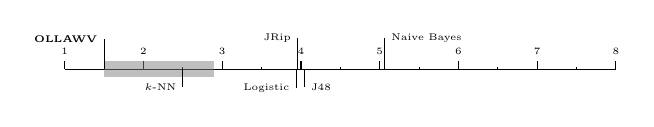
\begin{tikzpicture}
\draw (1,0) -- (8,0);
\foreach \x in {1,2,3,4,5,6,7,8} {
\draw (\x, 0) -- ++(0,.1) node [above,scale=0.7] {\tiny \x};
\ifthenelse{\x < 8}{\draw (\x+.5, 0) -- ++(0,.03);}{}
}

\coordinate (c0) at (1.5,0);
\coordinate (c1) at (2.5,0);
\coordinate (c2) at (4.041,0);
\coordinate (c3) at (3.9583,0);
\coordinate (c4) at (5.0625,0);
\coordinate (c5) at (3.9375,0);

\node (l0) at (c0) [above left=.25cm and 0cm, align=right,scale=0.7] {\tiny \textbf{OLLAWV}};
\node (l1) at (c1) [below left=.1cm and 0cm, align=right,scale=0.7] {\tiny $k$-NN};
\node (l2) at (c2) [below right=.1cm and 0cm, align=right,scale=0.7] {\tiny J$48$};
\node (l3) at (c3) [above left=.25cm and 0cm, align=right,scale=0.7] {\tiny JRip};
\node (l4) at (c4) [above right=.25cm and 0cm, align=right,scale=0.7] {\tiny Naive Bayes};
\node (l5) at (c5) [below left=.1cm and 0cm, align=right,scale=0.7] {\tiny Logistic};


\fill[fill=gray,fill opacity=0.5] (1.5,-0.1) rectangle (2.89,0.1);

\foreach \x in {0,1,2,3,4,5} {
\draw (l\x) -| (c\x);
};
\end{tikzpicture}}
\captionsetup{width=\linewidth}
\captionof{figure}{Bonferroni-Dunn test for Accuracy}\label{fig:BonfDunnaccOther}
\end{minipage}
\end{table}

\begin{figure}
\centering
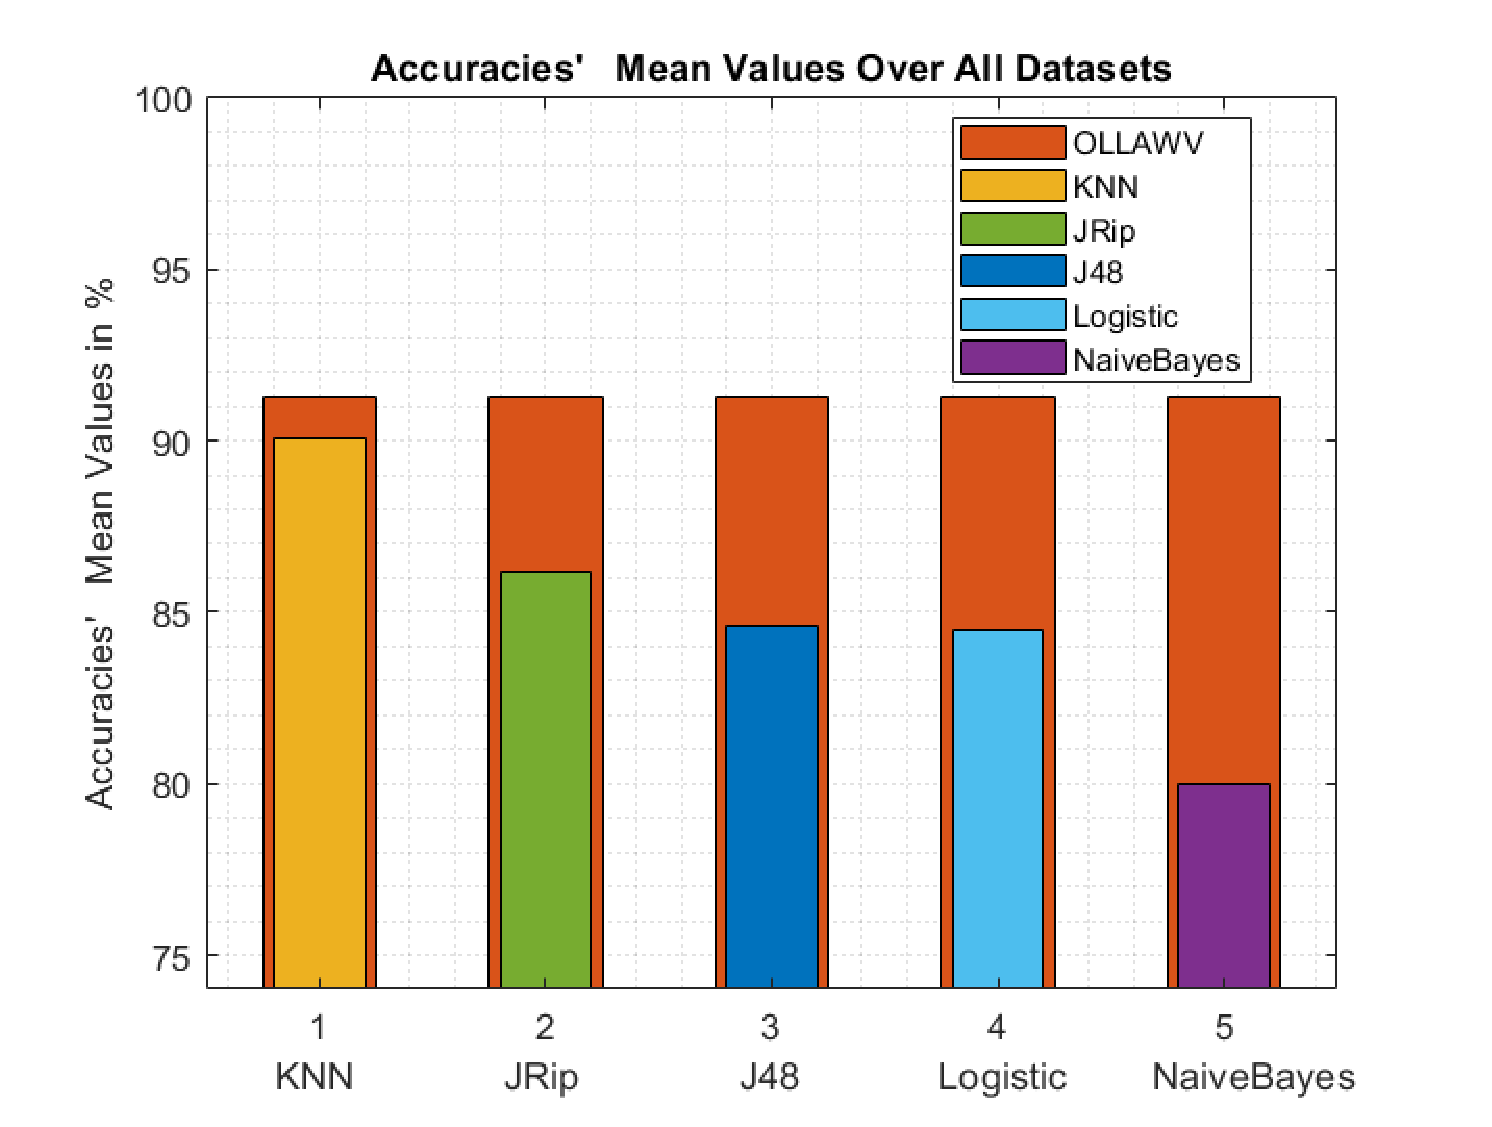
\includegraphics[width=0.6\textwidth]{figures/others.eps}
\caption{\small Mean accuracy over all datasets for OLLAWV and the 5 non-SVM state-of-the-art methods.}
\label{fig:accother}
\end{figure}
Table~\ref{tab:OtherResultsacc} displays the accuracy results for OLLAWV and five state-of-the-art methods. The table also shows the standard deviation for accuracy per outer fold, the average values accross all datasets, and the algorithm ranks. As the results indicate, OLLAWV outperforms all other state-of-the-art methods. Figure~\ref{fig:accother} displays the average accuracy results for OLLAWV and the non-SVM methods accross all datasets and highlights OLLAWV's better performance. The Friedman test indicates that OLLAWV performs significantly better than the competing methods for $\alpha = 0.05$ and is ranked first. Figure~\ref{fig:BonfDunnaccOther} shows the critical distance bar (which is $1.391$), and indicates that all other algorithms perform statistically significantly worse than OLLAWV, except for $k$-NN. 

\section{Conclusions}\label{sec:ollawvconclusion}
This paper proposed a novel online learning procedure and algorithm for solving the L1-SVM problem, which is a unique method in terms of both iterating over samples and updating the model. A new stopping criterion for the stochastic gradient procedure is also proposed. The model is updated by changing the weight $\alpha_i$ of a single worst-violator per iteration and stops when all violating samples i.e., support vectors, are found. Finding the \textit{worst-violators} is done without replacement. Such an approach results in a significant shortening of training time, as well as in a huge decrease in the resulting model size. The key features of the proposed algorithm, OLLAWV, stem from its implicit ability of finding support vectors and its self-stopping condition. This design was devised to address the limitations presented by current SVM solvers. 

The first experimental study demonstrates the better performance of OLLAWV compared with state-of-the-art SVM solvers (MNSVM and NNISDA) which have been shown to outperform the popular SMO implementation in the LIBSVM package. The results for accuracy, runtime, and percentage of support-vectors, obtained by the strict nested cross-validation procedure, were compared and further validated using statistical analysis with non-parametric tests. They highlighted the advantages and major speedup achieved by OLLAWV against the competing MNSVM and NNISDA. The second, supplemental experimental study evaluated the performance of OLLAWV against $5$ popular non-SVM methods, showing the better performance of OLLAWV against all five non-SVM algorithms ($k$-Nearest Neighbors ($k$-NN), J48, JRip, Na\"ive Bayes, and Logistic). The proposal, OLLAWV, performs statistically better in terms of runtime and model size across all $23$ evaluated benchmark datasets, without compromising accuracy. The research outcomes of this chapter have been published in~\cite{melki2018ollawv}.

\chapter{OLLAWV for Batched Data Streams}
Due to advances in hardware and software technologies, data generation and automated storage has become fast, voluminous, and continuous; usually referred to as streams of data. Nowadays, data streams are ubiquitous and notoriously difficult to store, analyze, visualize, and learn from. Most traditional machine learning techniques need to be adapted to accommodate the streamed, also known as online, environment due to underlying resource constraints, i.e. memory consumption and runtime, as well as the possibility of concept drift. This chapter presents a novel implementation and experimental environment for two online support vector machines (SVMs) in the batched data stream setting. Unlike other existing methods, these two online algorithms were chosen because their characteristics are a natural remedy for the time and memory constraints that come with the data stream problem. The first algorithm's low memory complexity deals with the memory constraints, and the second methods' fast runtime and self-stopping capability remedies the time constraint. The results for the latter, \textit{OnLine Learning Algorithm using Worst-Violators} (OLLAWV), showed a superior performance to the former, \textit{OnLine Learning Algorithm - List 2} (OLLA-L2). OLLAWV was then compared to 12 popular data stream algorithms against 24 datasets and stream generators. The results and statistical analysis showed OLLAWV's better performance, making it suitable for streamed learning. 

\section{Data Stream Classification Background}
This section first defines the notation that will be used throughout the chapter, and then formally describes the data stream classification problem along with relevant popular algorithms used within this paradigm.

\subsection{Notation}
\begin{table}[t!]
\small \centering
\caption{Summary of Data Stream Notation}\label{tab:NotationDS}
\begin{tabularx}{\textwidth}{l@{\extracolsep{\fill}}l}
\hline\noalign{\smallskip}
Definition & Notation\\ 
\noalign{\smallskip}\hline\noalign{\smallskip}
Number of Samples & $n$ \\
Number of Input Attributes & $d$ \\
Time Step & $t$ \\
\noalign{\smallskip}\hline\noalign{\smallskip}
Data Generating Process & $\proc = \set{(\bm x_1,y_1), (\bm x_2,y_2), \ldots, (\bm x_t,y_t), \ldots}$ \\
Set of Samples Provided to the Algorithm & $\mathcal{S}_t = \set{\tup{\bm x_t^1,y_t^1},\ldots,\tup{\bm x_t^n,y_t^n}} = \set{(\bm{X}_t,\bm{Y}_t)} \in \proc$ \\
\noalign{\smallskip}\hline\noalign{\smallskip}
Input Space at time $t$ & $\bm{X}_t \in \mathbb{R}^{n \times d}$ \\
Labels at time $t$ & $\bm{Y}_t \in \ints^n$ \\
Sample $i$ at time $t$ & $\bm{x}_t^i = (x^{i1}_t, \ldots, x_t^{id}) \in \bm X_t,\, \forall i \in \set{1,\ldots,n}$ \\
Sample Label $i$ at time $t$ & $y_t^i \in \bm Y_t,\, \forall i \in \set{1,\ldots,n}$ \\
\noalign{\smallskip}\hline
\end{tabularx}
\end{table}

Let $\proc$ be a data generating process which provides a sequence of tuples $\mathcal{S}_t = \set{\tup{\bm x_t,y_t}}^n$ that are sampled from an unknown probability distribution at some arbitrary time $t$, where $n$ is the number of tuples. The sub-script, time $t$, is used to explicitly assert the data's possible time-varying nature. $\bm x_t \in \reals^d$ represents a feature vector, and $y_t \in \ints$ is its discrete class label (in the non-binary classification case), both at time time $t$. The data may arrive to the algorithm in an online manner, i.e. one sample at a time: $\mathcal{S}_t = \set{\tup{\bm x_t,y_t}}$, or in a batch setting: $\mathcal{S}_t = \set{\tup{\bm x_t^1,y_t^1},\ldots,\tup{\bm x_t^n,y_t^n}}$. The single-sample setting occurs when $n = 1$.

\subsection{Data Stream Classification Methods}
In the context of supervised data stream classification, the goal is to learn the relationship between a set of attributes and a class label from continuous and rapidly arriving data. Examples of real-world data stream applications range between network analysis, financial data prediction, traffic control, sensor measurement, GPS tracking, as well as many others~\cite{moacite,gaber2007survey,krawczyk2017ensemble}. A data generating process, $\proc$, produces a rapid sequence of data, $\mathcal{S}_t$, either in \textit{batches} or in an \textit{online} format, from an unknown distribution, over time $t$ that is possibly infinite in length and cannot be accessed more than once~\cite{zang2014comparative}. In real-world scenarios, $\mathcal{S}_t$ is only available for learning at the time it is first presented to the algorithm~\cite{bifet2009new}. This requires machine learning algorithms to be robust, alert, and perform classification in a resource adaptive way. The stream would need to be classified on demand, since there is no way to control the arrival of test samples. 

Typically, there are two main core categories of data streams: \textit{stationary} streams, where the samples are drawn from a fixed, unknown probability distribution, and \textit{non-stationary} streams, where data distribution can change over time. In the non-stationary case, the class labels and/or attribute distributions can evolve, abruptly or gradually. This phenomenon is called \textit{concept drift}. These drifts are only apparent in incoming samples, which will eventually cause the classifiers performance to deteriorate, due to being trained on outdated training data. Besides gradual and abrupt (i.e. sudden) changes, concept drifts can also be described by their continuity, predictability, and recurrence~\cite{krawczyk2017ensemble,webb2016characterizing}. Stationary stream classifiers lack any mechanism to adapt quickly when a drift occurs. Due to these complexities, in both the stationary and non-stationary case, fast, robust, and adaptive algorithms need to be designed for the data stream environment. 

There are two main approaches for data stream learning problems in non-stationary environments: \textit{active} and \textit{passive}. To accommodate possible changes in the data stream, as well as ensure prompt and robust classification, passive approaches, also known as \textit{trigger}, perform continuous updates of the model whenever new data arrive. The active approach relies on a \textit{change-detection} mechanism which triggers an update to remedy or react to the change encountered. Both approaches attempt to maintain an updated model at all times, however, passive approaches can avoid potential errors that might arise by a faulty change-detection mechanism (false alarms or failures to detect changes)~\cite{ditzler2015learning}. Methods that fall under the passive approach are typically divided into two main categories: those that focus on updating a single classifier (\textit{Single Classifier Models}), and those that add/remove/modify components of ensemble models (\textit{Ensemble Classifier Models}). Single classifier models usually provide a lower computational cost, in comparison to ensemble models, making them a more attractive and simple solution for mining ultra-large data streams. However, ensemble methods are very popular due to their natural way of handling drifting streams~\cite{krawczyk2017ensemble}. 

One of the earliest passive methods, specifically designed for the streaming environment, is the popular \textit{Very Fast Decision Tree} (VFDT)~\cite{domingos2000mining}, or \textit{Hoeffding Tree}. It essentially sub-samples data to achieve scalability when constructing the tree. The main idea behind this approach is to determine a representative sample of sufficient size for constructing the tree, as though it were constructed on the entire dataset. It was transformed to accommodate the data stream format by building the tree incrementally. In order to accommodate concept-drifting streams, the method was extended in~\cite{hulten2001mining} and is called \textit{Concept-adapting Very Fast Decision Tree} (CVFDT). It was also extended to handle multiple sub-trees at each node. Gama et. al.~\cite{gama2006decision} also modified the VFDT method to handle continuous and drifting data by applying Bayes classifiers at leaf nodes~\cite{aggarwal}. Another more recent adaptation of VFDTs is the \textit{Hoeffding Option Tree} (HOT)~\cite{pfahringer2007new}, which enables each training sample to update a set of option nodes, instead of a single leaf. One of the major disadvantages of the VFDT family is that they are naturally suited for categorical data. Numerical data would need to be discretized; a task that is usually done offline. It is possible to test all possible splits, however, when dealing with numerical data, the number of splits may be very large. 

Rule-based methods have also been adapted for the data stream environment because of their high level of interpretability. One popular example of a rule-based method is the \textit{Very Fast Decision Rules} (VFDR)~\cite{gama2011learning} algorithm. This approach uses Na\"{i}ve Bayes to help exploit information available in each rule. Rule classifier's major disadvantage lies when data evolves significantly because of their inability to adapt quickly~\cite{ditzler2015learning}. 

%\textit{Na\"{i}ve Bayes}~\cite{john1995estimating} is a well-known classifier that simply updates internal counters based on new incoming samples and then uses the counters to probabilistically assign class labels to unknown samples. It is a good baseline in terms of speed, however, it has been outperformed by VFDTs~\cite{domingos2000mining}.

Ensemble classifiers are popular approaches for learning in streamed environments and provide some advantages: they tend to have more flexibility in easily incorporating newly presented data into a model by adding new members to the ensemble. They also obtain a natural way of ``\textit{forgetting}" irrelevant knowledge by removing members from the ensemble~\cite{ditzler2015learning}. The two most common ensemble methods are bagging and boosting~\cite{oza2001onlinebb}. One well know, online approach that uses sample and model weighting/selection to obtain the best accuracy over different sections of a drifting stream is the \textit{Dynamic Weighted Majority} (DWM)~\cite{kolter2007dynamic} algorithm. The main idea is to choose the best weighted classifier that performs well for an unseen sample, or portion of the training stream, while having the ability to add/remove classifiers to accelerate reacting to a possible drift. Another ensemble method is the \textit{Social Adaptive Ensemble 2} (SAE2)~\cite{gomes2014sae2}, an improved version of SAE~\cite{gomes2013sae} classifier. The main difference between the two is that SAE2 implements a more scalable adaptation method. Another relatively new online ensemble is the \textit{Anticipative Dynmic Adaptation to Concept Changes} (ADACC)~\cite{jaber2013new} algorithm, which recognizes concepts from incoming samples and optimizes control over the incremental classifiers. The main disadvantages of such ensemble approaches stem from their high computational and spacial complexity, as well as their low inter-classifier interpretability.

Another ensemble approach, belonging to the Learn++ family of algorithms~\cite{polikar2001learn}, is the method called \textit{Learn++ for Non-Stationary Environments} (Learn++.NSE)~\cite{elwell2011incremental}. Unlike the previously mentioned ensemble methods, Learn++.NSE operates in batch mode, and has the ability to learn from environments that exhibit a constant, variable, or cyclical drifts. It uses a time-adjusted loss function to favor newly trained classifiers, as well as classifiers that have performed will in the past (in case of a recurring concept). 

\textit{$k$-Nearest neighbor} ($k$-NN) methods comprise another set of algorithms that have been adapted to handle non-stationary streams of data, however, they use a \textit{change-detection} mechanism. Unlike the VFDTs and Na\"{i}ve Bayes classifiers, $k$-NN cannot learn from a stream without discarding data. These methods maintain a dynamic sample, or \textit{sliding window}, of the data stream. Finding this representative sample of data is referred to as \textit{reservoir sampling}~\cite{vitter1985random}, a technique used by many streaming algorithms~\cite{ditzler2015learning}. Basic implementations of $k$-NN maintain a sliding window of fixed sizes because storing all samples in a stream is not feasible due to memory and processing constraints. The class label is then assigned by the majority label present among the $k$-nearest neighbors of the unknown test sample. 

An example of such windowing methods is the \textit{Probabilistic Adaptive Window} (PAW) algorithm, used with $k$-NN in~\cite{bifet2013efficient}. Rather than storing all samples, or a limited sized window, PAW keeps a dynamically sized window with a logarithmic number of samples, storing those with higher probability than the rest. Another example of windowing techniques is that of the \textit{ADaptive WINdowing} (ADWIN) algorithm~\cite{bifet2007learning}, which increases the size of the window when no change is apparent, and shrinks it when there is a drift. The main disadvantage with these change detection techniques is their difficulty to set a threshold for when a change occurs; too low of a threshold value would cause many false positives, and too large a threshold would cause many false negatives. 

Other widely used examples of change-detection techniques include the \textit{Drift Detection Method} (DDM)~\cite{gama2004learning} and its improvement \textit{Early Drift Detection Method} (EDDM)~\cite{baena2006early}. DDM estimates the classifier error, which must decrease as more training samples arrive. However, if the classification error increases above some threshold, a warning signal is generated and new incoming samples are then stored in a window. If the error later falls below the threshold, the warning is considered a false alarm and the window is discarded. If the error rate increases, the classifier is then rebuilt on the samples stored in the window. EDDM is similar to its predecessor, however offers an improvement for detecting gradual drifts by proposing a novel method for comparing distances of error rates.

Support vector machine (SVM) methods have infrequently been used for data stream classification due to challenges that stem from incrementally updating the SVM model as the number of samples increases. Some methods, such as \textit{SVMLight}~\cite{Joachims1999} and \textit{SVMPerf}~\cite{joachims2006training}, have been proposed for speeding up SVM classification. It is worth noting that some of the earliest work in streamed SVM learning~\cite{klinkenberg2000detecting,syed1999handling} precedes the earliest work in stream decision tree learning. In fact, the contributions made by Klinkenberg and Joachims in~\cite{klinkenberg2000detecting}, are one of the earliest window-based methods for detecting concept drift. Other significant contributions on incremental and online (sotchastic) support vector machines are discussed in~\cite{bordes2005fast,cauwenberghs2001incremental,domeniconi2001incremental,fung2002incremental,ralaivola2001incremental,ruping2001incremental,shilton2005incremental}.

However, the biggest issue with these algorithms is that most were not designed for streaming environments. Adjusting SVMs for the data stream setting is a particularly critical task because of their generalization capabilities, scalability, and robustness against outliers. Most of the methods mentioned employ a quadratic programming formulation, with equal number of constraints as the number of data, making the problem computationally expensive for large amounts of data. In the kernelized case, the size of the kernel scales with the number of samples squared, an impractical solution in the case of data streams. Even when using decomposition methods, the disadvantage then stems from receiving an approximate solution; which may require the algorithm to make many passes over the data to achieve a reasonable level of convergence. Condisering the event of a concept drift, the Karush-Kuhn-Tucker (KKT) optimality conditions must be maintained if/when adding or removing samples for the algorithm to succeed~\cite{aggarwal}. The most interesting SVM methods for data stream learning are that of Cauwenberghs and Poggio~\cite{cauwenberghs2001incremental}, and Bordes et al.~\cite{bordes2005fast}, because both utilize decremental unlearning methods which provide insights into the relationship between the geometry of the data and generalization capabilities.

These computational, spacial, and time complexities are what prompted researchers to investigate large-scale learning solutions using \textit{Stochastic Gradient Descent} (SGD) before investigating how to deal with concept-drifts and their detection~\cite{herbrich2016learning,kivinen2002large,rosenblatt1958perceptron,Schoelkopf2002,Shalev2014,shalev2011pegasos}. Stochastic algorithms can be both the fastest and have superior generalization performances~\cite{bousquet2008tradeoffs,kivinen2004online} against batch methods. This (and the work done in~\cite{Melki2016,kecman2016ieee}) prompted the investigation of the novel \textit{OnLine Learning Algorithm} (OLLA)~\cite{kecman2016fast} and its younger counterpart \textit{OnLine Learning Algorithm using Worst-Violators} (OLLAWV)~\cite{melki2018ollawv} under a stationary and non-stationary data stream environment. Due to their online, iterative nature, and that they have shown significant improvements over popular SVM solvers in terms of speed, memory consumption, and accuracy; OLLA and OLLAWV are a natural extension for SVMs to the data stream environment.

\newpage
\section{OnLine Learning Algorithms for Batched Data Streams}
OLLA-L2~\cite{kecman2016fast} and its successor OLLAWV~\cite{melki2018ollawv} are two online, iterative learning algorithms that are implemented and investigated within the context of a batched, stationary and non-stationary, data stream environment. OLLA-L2 stems from the same core algorithm as OLLAWV, named \textit{OnLine Learning Algorithm} (OLLA)~\cite{kecman2016fast}. It is a generic stochastic learning algorithm tailored and designed for various non-linear (i.e. kernel) classifiers in the primal domain. In this implementation of OLLA-L2, similar to that of OLALWV described in Chapter~\ref{chap:ollawv}, the online learning algorithm is derived and used for solving the primal L1-SVM cost function, given by Equation~\ref{eqn:reghingeloss}. The online nature of the core OLLA algorithm and its superior performance in terms of speed and accuracy against popular and widely used SVM solvers merited investigation in the data stream setting. The main objective is to design a novel base-line incremental support vector machine that is capable of handling large volumes of streamed data in a short amount of time, while maintaining a competitive accuracy. By beginning with this approach, in the event of a concept drift, the classifier would simply be able to rebuild itself, without violating any time constraints. 

The algorithm that was first implemented and investigated under the data stream environment was OLLA-L2, listed in Algorithm~\ref{alg:List2L1SVM}. At every iteration, OLLA-L2 proceeds cyclically over the data, updating the model if the chosen sample, $i$, is a violator, i.e. has an error $y_i o_i \leq 1$, where $y_i$ and $o_i$ are the sample's class label and corresponding model output, respectively. If the sample has no error ($y_i o_i > 1$), the model remains the same and no update is performed. Note, this error rule is that of the Hinge loss, shown in Equation~\ref{eqn:hingeloss}. In the context of batched streams, the algorithm would cycle through the samples in each arriving batch. For a pure online scenario, the algorithm would proceed with its updates, as long as samples are provided by the stream. 

The update parameters $\Lambda \in \reals$ (lambda) and $\Rho \in \reals$ (rho), as seen in Algorithm~\ref{alg:List2L1SVM}, describe scalars which are used for updating the output vector $\bm o \in \reals^n$, the weight vector in kernel feature space $\bm \alpha \in \reals^n$, and the bias term $b \in \reals$, if used. The input parameter $\beta \in \set{0,1}$ describes whether the bias term will be used ($\beta = 1$) or not ($\beta = 0$). The update parameters for $\Lambda$ and $\Rho$ for the L1-SVM with regularizer $||\bm w||^2$ are given by:
\begin{table}[H]
\centering \small
\begin{tabular}{cc}
$\Lambda = \eta C y_i$ & $\Rho = \eta \alpha_i$
\end{tabular}
\end{table}

The advantage of using OLLA-L2's update procedure is most apparent in lines 8 and 15 in Algorithm~\ref{alg:List2L1SVM}. The model's $\bm \alpha$ parameter update is simply the sum of two scalars values: the previous value of $\bm \alpha$ and $\Lambda$. Then, to determine whether an update is even needed, the next sample's output value, $o_i$, is needed. It is obtained by using the scalar product of kernel values and weight vector $\bm \alpha$ for support vectors (stored in $\bm S$) only. Hence, the sparser the model, the more OLLA-L2 exhibits a speed-up~\cite{kecman2016fast}. 
\begin{algorithm}[t!]
\centering \small
\caption{OnLine Learning Algorithm - List 2 (OLLA-L2)}
\label{alg:List2L1SVM} 
\begin{algorithmic}[1]
\renewcommand{\algorithmicrequire}{\textbf{Input:}}
\renewcommand{\algorithmicensure}{\textbf{Output:}}
\Require $\bm X, \bm Y, \beta, n, e$
\Ensure  $\bm \alpha$, $b$, $\bm S$
\State $\bm \alpha \leftarrow \bm 0, b \leftarrow 0, \bm S \leftarrow \bm 0,\, \bm o \leftarrow \bm 0,\, i \leftarrow 0$
\For{$t = 1, \ldots, n*e$}
\State $\eta \leftarrow 2/\sqrt{t}$
\If{$Y_i\, o_i \leq 1$}
\State \textit{Calculate $\Lambda$ and $\Rho$}
\State $\bm S \leftarrow [\bm S \cup i]$
\State $\alpha_i \leftarrow \alpha_i + (\Lambda - \Rho)$
\State $b \leftarrow b + (\Lambda - \Rho)\beta$
\EndIf
\State $i \leftarrow i + 1$
\If{$i = n$}
\State $i = 0$
\EndIf
\State $o_i \leftarrow \bm{K}(\bm x_i,\, \bm x_{\bm S})\, \bm \alpha_{\bm S} + b$
\EndFor
\end{algorithmic} 
\end{algorithm}

In the batch setting, the quantity of iterations can be controlled by the parameter $e$, which represents the number of epochs, or cycles, over the data. As mentioned in the previous chapter, early stopping acts as a regularization technique~\cite{collobert2004links}. It is worth noting that, if the number if epochs is set to be less than the number of samples, or in the pure online stream learning setting, where samples arrive one at a time with no cycling involved, the parameter $\Rho$ is always equal to 0 because $\bm \alpha$ is initialized to 0. $\Rho > 0$ only if the algorithm cycles over samples that have already had their respective $\bm \alpha$ updated.

To try and maintain a sparse model, especially with evolving data streams, is a difficult task. In the context of batch data streams, building a new model from scratch might be too expensive, especially if there are many support vectors. The sample principle applies to the pure online scenario. Because of these issues, a simple change detection mechanism was designed and tested. OLLA-L2 was first updated to store the classification error, $\bm \xi = \sum_{i=1}^n y_i\, o_i$, for each previous batch trained on. If the mechanism is used, upon receiving a new batch of data, the algorithm will calculate the difference in error between subsequent batches and make a decision to either do nothing, update, or completely rebuild the model. The model update procedure involves firstly training the model on the new batch, then eliminating the support vectors with the smallest $\bm \alpha$ values, and then appending the newly added support vectors. Model variables from previous batches are scaled down by a `learning rate' that set to be large for the older batches and smaller for the more recent ones. This gives preference to newly arriving samples in the case of a drift. 

Although OLLA-L2 has many advantages, it also has complexities, some of which are shared by other stochastic solvers. One example would be how/what to set the algorithm's maximum number of iterations, i.e. the model's optimal point to stop training. Stopping the training process prematurely might cause a missed opportunity for finding all possible support vectors. Stopping too late might cause the algorithm to diverge from its optimum point, while leading to a longer runtime. Setting a stopping point for training would be especially difficult for the pure online scenario. This complexity inspired the work in Chapter~\ref{chap:ollawv} on OLLAWV. The novelty and advantage of OLLAWV resides in the way it iterates and updates the model. At each step, the algorithm chooses and updates the most violating sample, i.e. \textit{worst-violator}. A worst-violator is defined as the sample that produces the largest error with respect to the current decision function. Rather than shuffling the data and cycling through each sample, as done in OLLA-L2, OLLAWV selects (without replacement) the most incorrectly classified sample and updates the model accordingly. This procedure essentially finds the model's support vectors while implicitly defining a stopping criterion: if there are no more violating samples, the algorithm terminates. These characteristics are especially useful in the context of learning from a batch streamed environment since the resulting model is speedily trained and is always sparse~\cite{melki2018ollawv}. 
\begin{table}[t!]
\centering
\caption{Comparison of OLLAWV vs. OLLA-L2}
\scriptsize
\label{tab:dslvsolla}
\resizebox{\textwidth}{!}{\begin{tabularx}{\textwidth}{l@{\extracolsep{\fill}}cccc}
\noalign{\smallskip}\hline\noalign{\smallskip}
\multicolumn{1}{l}{Dataset} & \multicolumn{2}{c}{Accuracy (\%)} & \multicolumn{2}{c}{Runtime (s)} \\
\cmidrule(lr){2-3}
\cmidrule(lr){4-5}
 & OLLA-L2 & OLLAWV & OLLA-L2 & OLLAWV \\
\noalign{\smallskip}\hline\noalign{\smallskip}
RBFNoDrift &93.0663 &\textbf{94.2117} &\textbf{0.02379} &0.0329   \\
HyperplaneSlow &87.4016 &\textbf{90.0913} &\textbf{0.0261} &0.0353   \\
HyperplaneFaster &87.4033 &\textbf{89.5092} &\textbf{0.0256} &0.0263   \\
STAGGERGeneratorF1 &\textbf{100.000} &\textbf{100.000} &0.0034 &\textbf{0.0021}  \\
HyperplaneFaster02 &87.4047 &\textbf{89.4911} &\textbf{0.0257} &0.0268   \\
MixedGeneratorBT &92.4990 &\textbf{97.9969} &\textbf{0.0108} &0.0205  \\
MixedGeneratorBF &92.5537 &\textbf{98.0284} &\textbf{0.0107} &0.0299   \\
SineGeneratorF1BF &97.3659 &\textbf{97.7909} &\textbf{0.0091} &0.0122   \\
SineGeneratorF2BF &97.3659 &\textbf{97.7909} &\textbf{0.0091} &0.0121   \\
STAGGERGeneratorF1BF &\textbf{100.000} &\textbf{100.000} &0.0035 &\textbf{0.0021}   \\
STAGGERGeneratorF2BF &\textbf{100.000} &\textbf{100.000} &0.0039 &\textbf{0.0022}  \\
HyperplaneFasterAN0 &87.4033 &\textbf{89.5092} &\textbf{0.0255} &0.0263   \\
HyperplaneFasterAN5 &87.2912 &\textbf{89.2898} &\textbf{0.0258} &0.0264   \\
SEASuddenAN0 &84.0088 &\textbf{87.7956} &0.0494 &\textbf{0.0208}   \\
SEASuddenAN05 &83.6874 &\textbf{87.5283} &0.0494 &\textbf{0.0284}  \\
\noalign{\smallskip}\hline\noalign{\smallskip}
Average &91.8300 &\textbf{93.9356} & \textbf{0.0201} & 0.0203 \\
Rank & 1.9 &\textbf{1.1} &\textbf{1.3333} & 1.6667  \\
\noalign{\smallskip}\hline\noalign{\smallskip}
\end{tabularx}}
\end{table}

Preliminary experiments were conducted to test the capabilities of both approaches, and the results for percent accuracy and runtime are listed in Table~\ref{tab:dslvsolla}. The results show the better performance of OLLAWV in terms of accuracy. Both algorithms scale similarly in terms of runtime. The fast comparative runtime of OLLAWV-L2 is dependent on its change detection mechanism, since models have the opportunity to be minimally updated, or even remain the same over new incoming batches of data. However, OLLAWV achieves a competitive runtime without the use of a change detector. The main bottleneck in terms of runtime for OLLAWV is the kernel vector calculation needed for calculating the model output $\bm o$, i.e. current decision function output. Only non-support vector output values are calculated per iteration because samples are only allowed to be updated once. Therefore, the number of kernel calculations decreases by 1 per iteration. This phenomenon, as well as early stopping are contributing factors to OLLAWV's competitive runtime and model sparsity. These characteristics motivated OLLAWV's implementation and further experimentation in the context of batch data streams.


\newpage
\section{Experimental Environment, Results, and Analysis}
This section presents the experimental setup and comparison of OLLAWV against 12 popular data stream algorithms on 24 different benchmark datasets and stream generators. The experimental setup is first described, the contemporary comparison methods are then listed, then a brief description of the datasets and stream generators is presented. The results over several metrics, as well as statistical analyses are then shown and the overall performance of the algorithms are discussed. The main purpose of OLLAWV's implementation in a data stream environment and the following experiments was to investigate whether it is capable of learning from streams efficiently, ensuring a strong base algorithm before tackling streams with abrupt concept drift. 

\subsection{Experimental Environment} %The experiments were conducted over 24 different data streams. 
The experimental environment was designed to test the difference in performance of the proposed method against 12 contemporary algorithms which are designed to handle stationary and non-stationary data streams. Some use explicit drift-detector mechanisms and others take a passive approach. The majority of the classifiers used in the experiments are without an explicit concept-drift detector because OLLAWV was implemented without one, ensuring a fair comparison. However, classifiers with a drift detector were included for a more comprehensive understanding of how OLLAWV will compare. 

\begin{table}
\caption{Data Stream Algorithm Summary} \centering \footnotesize
\label{tab:dsalgs}
\begin{tabularx}{\textwidth}{l@{\extracolsep{\fill}}lcc}
\hline\noalign{\smallskip}
Algorithm 	& Description 									&    Passive	&   Active  		\\
\noalign{\smallskip}\hline\noalign{\smallskip}
HOT~\cite{pfahringer2007new} 	& Hoeffding Option Tree 	&	\checkmark	&					\\
AdaHOT~\cite{pfahringer2007new} & AdaHoeffding Option Tree 	&	\checkmark	&					\\
NB~\cite{john1995estimating}	& Na\"{i}ve Bayes 			&	\checkmark	&					\\
$k$-NNPAW~\cite{bifet2013efficient}	& $k$-NN with Probabilistic Adaptive Windows & \checkmark & \\
EDDM~\cite{baena2006early} 		& Early Drift Detection Method  &			&	\checkmark		\\
VFDR~\cite{gama2011learning} 	& Very Fast Decision Rules 	&	\checkmark	&					\\
VFDR-NB~\cite{gama2011learning} & VFDR with Na\"{i}ve Bayes	&	\checkmark	&					\\
SAE2~\cite{gomes2014sae2}		& Social Adaptive Ensemble 	&	\checkmark	&					\\
Learn++.NSE~\cite{elwell2011incremental} & Learning in Non-Stationary Environments &\checkmark &\\
DWM~\cite{kolter2007dynamic} 	& Dynamic Weighted Majority &				&	\checkmark		\\
DACC~\cite{jaber2013new}		& Dynamic Adaptation to Concept Changes  	& &	\checkmark		\\
OCBoost~\cite{pelossof2009online} & Online Coordinate Boosting 	&	\checkmark	&			\\
\noalign{\smallskip}\hline
\end{tabularx}
\end{table}

%\textit{The algorithms without a drift detector are as follows: \textit{Hoeffding Option Tree} (HOT)~\cite{pfahringer2007new}, \textit{Adaptive Hoeffding Option Tree} (AdaHOT)~\cite{pfahringer2007new}, \textit{Na\"ive Bayes}, \textit{Rule Classifier} (RC) and \textit{Rule Classifier Na\"ive Bayes} (RCNB)~\cite{gama2011learning}, \textit{Social Adaptive Ensemble Classifier} (SAE2)~\cite{gomes2014sae2}, and \textit{Online Coordinate Boosting} (OCBoost)~\cite{pelossof2009online}. Those with a drift detector are: \textit{$k$-Nearest Neighbors with Probabilistic Adaptive Window} ($k$-NNPAW), \textit{Single Classifier Drift} (SCD)~\cite{baena2006early} using the \textit{Hoeffding Tree} as a base, \textit{Learning in Non-Stationary Environments} (Learn++.NSE)~\cite{elwell2011incremental}, \textit{Dynamic Weighted Majority} (DWM)~\cite{kolter2007dynamic}, \textit{Dynmic Adaptation to Concept Changes} (DACC)~\cite{jaber2013new}.}

These algorithms were chosen because they have shown considerable performance in learning in a stream environment, while also being readily available for use and reproducing their results through MOA, \textit{Massive Online Analysis}\footnote{https://moa.cms.waikato.ac.nz/}~\cite{moacite} framework. The experiments were run on a server with 2 Intel Xeon CPU E5-2690v4 with 28 cores (56 threads), 128 GB of memory, and CentOS 7.4. OLLAWV was also implemented in Java within MOA framework. 

\begin{algorithm}[t!]
\centering \small
\caption{Evaluate Interleaved Chunks}
\label{alg:evalChunk} 
\begin{algorithmic}[1]
\renewcommand{\algorithmicrequire}{\textbf{Input:}}
\renewcommand{\algorithmicensure}{\textbf{Output:}}
\Require $\proc = \set{\mathcal{S}_1,\ldots,\mathcal{S}_T}$
\Ensure  $\mathtt{evaluator}$
\State $\mathtt{firstChunk =\,TRUE}$
\State Initialize the $\mathtt{classifier}$ and $\mathtt{evaluator}$
\While{$\proc \neq \emptyset$}
\State From $\proc$ generate new batch of instances, $\mathcal{S}_t$
\If{!$\mathtt{firstChunk}$}
\For{$\forall (\bm x_t,\, y_t) \in \mathcal{S}_t$}
\State $\mathtt{double[]\,\,pred = classifier.classify(}(\bm x_t,\, y_t)\mathtt{)}$ 
\State $\mathtt{evaluator.addResult(}(\bm x_t,\, y_t)\mathtt{, pred)}$
\EndFor
\Else 
\State $\mathtt{firstChunk =\,FALSE}$
\EndIf
\State $\mathtt{classifier.trainOnInstances(}\mathcal{S}_t\mathtt{)}$
\EndWhile
\end{algorithmic} 
\end{algorithm}
In the context of traditional batch learning, the most popular and unbiased method for estimating the performance of an algorithm is the \textit{nested cross-validation} procedure. However, in the online learning setting which has computationally strict requirements and drifting concepts, the nested cross-validation procedure is not straightforwardly applicable. The approach taken for this experimental environment is the evaluation method named \textit{Interleaved Test-Then-Train}, also known as \textit{Prequential}~\cite{gama2013evaluating} (predictive sequential evaluation), listed in Algorithm~\ref{alg:evalChunk}. It is used to describe the change in accuracy (or any other evaluation metric) of algorithms over time. It follows the online learning protocol: when a sample is received, the current model makes a prediction, and when the system receives the sample's true label, the classifier's loss can be computed. In other words, each sample can be used to test the model before it is used during training, and using this, the evaluation metric can be incrementally updated. Using this order, the algorithms are always being tested on unseen samples. This scheme ensures that no hold-out test set is needed, thus utilizing all available data. It also provides a smooth and unbiased plot of the evaluation metric over time, where each sample becomes increasingly less significant to the overall average. 

Along with the prequential evaluation method, traditional $k$-fold cross-validation was used in the OLLAWV experiments for the purpose of model selection. Once a new batch is received by the algorithm, $5$-fold cross validation is performed to select the best representative parameters for the current batch, and once they are chosen, they will be used for the remaining batches. This rigorous procedure is computationally expensive, however, the goal is to optimally and fairly find the best representative SVM parameters for the incoming stream. First, each batch of samples is normalized by linear transformation of the feature values to the range [0,1]. Then the training process, also involving cross-validation and prequential evaluation, was performed. To deal with multi-class classification problems, the one-vs-one, or pairwise, approach was used. The best hyper-parameters were chosen from the following $6 \times 7$ possible combinations, shown in Equations~\eqref{eq:paramCollads} and~\eqref{eq:paramGollads}. 
\begin{subequations}
\label{eq:hyperparamollads}
\begin{align}
C \in \set{0.01, 0.1, 1.0, 10.0, 100.0, 1,000.0} \label{eq:paramCollads}\\
\gamma \in \set{0.01, 0.1, 0.5, 1.0, 2.0, 4.0, 16.0} \label{eq:paramGollads}
\end{align}
\end{subequations}
The $\gamma$ parameter refers to that of the Gaussian RBF kernel, given by:
\begin{equation}
\label{eq:rbfds}
\mathcal{K}(\bm{x_i},\bm{x_j}) = e^{-\gamma\norm{\bm{x_i} - \bm{x_j}}^2}.
\end{equation}


\subsection{Datasets}
\begin{table}[t!]
\caption{Base Streamed Datasets \& Generators}
\footnotesize
\centering
\label{tab:dsDataset}
\begin{tabularx}{0.9\textwidth}{l@{\extracolsep{\fill}}rrr}
\hline\noalign{\smallskip}
Dataset & \# Samples & \# Attributes & \# Classes \\
\noalign{\smallskip}\hline\noalign{\smallskip}
\textbf{\textit{Static}} 		&				&				& 		\\
Shuttle 						&    57,999		&   10 			& 	7 \\
Census							&   299,284     &  	42			& 	2 \\
CovType		 					&   581,012     & 	55			& 	7 \\
\textbf{\textit{Generators}} 	&				&				& 		\\
RandomRBFGenerator 	       	 	& 	1,000,000	& 	10	        & 	2 \\ %moa
LEDGenerator	 	       	 	& 	1,000,000	& 	2	        & 	10 \\ %moa
HyperplaneGenerator 	        & 	1,000,000	& 	10	        & 	2 \\ %
WaveformGenerator 	       	 	& 	1,000,000	& 	40	        & 	3 \\ %moa
STAGGERGenerator 	 			& 	1,000,000	& 	3	        & 	2 \\ %Incremental Learning from Noisy Data
MixedGenerator 					& 	1,000,000	& 	4	        & 	2 \\%Learning with drift detection.
SineGenerator 					& 	1,000,000	& 	2	        & 	2 \\%Learning with drift detection.
SEAGenerator	       			& 	1,000,000	& 	2	        & 	2 \\ %A streaming ensemble algorithm (SEA) for large-scale classification
\noalign{\smallskip}\hline
\end{tabularx}
\end{table}
Table~\ref{tab:dsDataset} presents a summary of the static datasets and the stream generators used throughout the experiments, where the number of attributes, classes, and samples are shown. Both the static datasets and the generators provided 1000-sample sized batches to the algorithms. The static datasets were obtained from the UCI Machine Learning repository\footnote{http://archive.ics.uci.edu/ml/index.php}~\cite{Lichman:2013} and were simulated as streams using a stream simulator from the MOA framework. The stream generators listed were also used within the MOA~\cite{moacite} framework. The following are descriptions of the types of generators used as base generators throughout the experimental study. Variations of the generators were also used to simulate the concept drift rate, as well as varying number of attributes, classes, and functions (pertaining to the functional generators). These variations are suffixed with the generator name in the results tables.
\begin{itemize}
\iitem \textbf{Random RBF Generator}: This generator produces samples that form normally distributed hyperspheres surrounding randomly selected centroids, with varying densities. This generator also has the option to simulate data evolution, i.e. concept drift. 

\iitem  \textbf{LED Generator}: This stream generator's goal is to predict the digit displayed on a seven-segment LED display, where each segment has a 10\% chance of being inverted.

\iitem \textbf{Rotating Hyperplane}: This generator produces samples of different classes that are separated by a hyperplane. Their orientation and position may be smoothly changed by modifying the size of the weights.

\iitem \textbf{Waveform Generator}: This generator constructs three different types of waves which are combinations of two/three base waveforms. The goal is to find the final wave type.

\iitem \textbf{STAGGER Concepts Generator}: This generator creates a concepts which are described by a collection of samples, where each sample is a boolean function of attribute-valued pairs and is described by a disjunct of conjuncts.

\iitem \textbf{MIXED Concepts Generator}: This stream generator has an abrupt concept drift, where the class label is selected based on some functional conditional, and is reversed after a context change.

\iitem \textbf{Sine Concepts Generator}: This generator involves two relevant attributes, each having values uniformly distributed between [0,1], with an abrupt concept drift change. In the first context, all samples below a sine curve are classified as positive. However, after the context change, the class label is reversed. 

\iitem \textbf{SEA Concepts Generator}: This generator involves an abrupt concept drift change and three attributes, of which only two are relevant, ranging between [0, 10]. Samples belong to a certain class label if the sum of the relevant attributes is less than or equal to some threshold value, which varies based on the concept. 

\end{itemize}

\section{Results \& Analysis}
The classification performance was measured using two metrics: Accuracy and Cohen's kappa rate, and the results are shown in Tables~\ref{tab:DSResultsacc} and~\ref{tab:DSResultskappa}, respectively. The metrics are calculated as shown in Equations~\ref{eq:accuracyds} and~\ref{eq:kappads}, where TP is the true positive value, TN is the true negative value, FP is the false positive value, FN is the false negative value, and $n^\prime = TP + FP + TN + FN$.
\begin{subequations}
\label{eq:metricsds}
\begin{align}
\text{Accuracy} \tab \tab &\dfrac{TP+TN}{n^\prime} \label{eq:accuracyds}\\[10pt]
\text{Cohen's Kappa Rate} \tab \tab &\dfrac{n^\prime - \dfrac{(TP+FN)*(TP+FP)}{n^\prime}}{1 - \dfrac{(TP+FN)*(TP+FP)}{n^\prime}} \label{eq:kappads}
\end{align}
\end{subequations}
The training times of each algorithm are also given in Table~\ref{tab:DSResultsTrain} to analyze the scalability of each of the algorithms. All metrics were calculated using the prequential procedure. 

In order to analyze the performances of the multiple models, non-parametric statistical tests are used to validate the experimental results obtained. The Iman-Davenport non-parametric test is run to investigate whether significant differences exist among the performance of the algorithms by ranking them over the datasets used, using the Friedman test. The algorithm ranks for each metric in Equations~\eqref{eq:metrics} are presented in the last row of the results tables, and the lowest (best) rank value is typeset in bold. 

After the Iman-Davenport test indicates significant differences, the Bonferroni-Dunn post-hoc test~\cite{Dunn1961} is then used to find where they occur between algorithms by assuming the classifiers' performances are different by at least some critical value. Below each result table, a figure highlighting the critical distance (in gray), from the best ranking algorithm to the rest, is shown. The algorithms to the right of the critical distance bar perform statistically significantly worse than the control algorithm, OLLAWV. Figures \ref{fig:BonfDunnaccDS}, \ref{fig:BonfDunnkappaDS}, and \ref{fig:BonfDunnTrainDS} show the results of the Bonferroni-Dunn post-hoc procedure over the metrics in Equation~\eqref{eq:metricsds}.

\begin{table}[H]
\caption{Accuracy (\%) Comparison for Data Stream Classifiers}
\scriptsize
\centering
\label{tab:DSResultsacc}
\resizebox{\textwidth}{!}{\begin{tabularx}{1.5\textwidth}{l@{\extracolsep{\fill}}ccccccccccccccc}
\noalign{\smallskip}\hline\noalign{\smallskip}
Dataset & OLLAWV & HOT & AdaHOT & NB & $k$-NNPAW & EDDM & VFDR & VFDR-NB & SAE2 & LearnNSE &DWM &DACC &OCBoost &\\
\noalign{\smallskip}\hline\noalign{\smallskip}
CovType &\textbf{90.2820} &85.3410 &86.2220 &60.0370 &87.8890 &59.5560 &60.3240 &75.5820 &76.2070 &69.9670 &71.9560 &61.7000 &71.2860 &  \\
census &93.7570 &94.6950 &\textbf{94.7350} &87.0190 &93.6460 &91.8530 &93.6480 &84.0600 &90.1320 &84.1440 &91.4040 &90.3710 &93.4690 &  \\
shuttle &98.6540 &98.1750 &98.5210 &90.0160 &\textbf{99.2640} &98.4890 &88.3980 &96.0570 &90.2430 &93.7890 &89.9120 &92.0270 &74.2110 &  \\
RBFNoDrift &\textbf{94.2120} &92.9410 &92.9600 &71.9920 &93.7470 &92.4790 &77.5290 &81.7070 &89.1610 &70.2820 &70.4250 &65.0080 &92.0840 &  \\
LEDNoDrift &73.8280 &73.8510 &73.8350 &\textbf{73.9420} &65.8280 &73.6380 &41.1620 &73.7520 &67.5960 &67.8400 &71.1460 &48.2680 &17.4400 &  \\
HyperplaneSlow &\textbf{90.0910} &82.0960 &82.4210 &77.6900 &84.0260 &81.5660 &68.8830 &85.1880 &82.6670 &86.2040 &88.0600 &80.6620 &85.7760 &  \\
HyperplaneFaster &\textbf{89.5090} &82.7170 &85.3420 &77.2310 &84.2720 &84.3260 &78.6330 &85.1810 &83.0130 &86.4990 &86.7610 &81.1540 &87.7950 &  \\
RBFGradualRecurring &98.4140 &94.6250 &94.4420 &58.3270 &\textbf{98.4260} &93.4690 &60.0800 &86.1600 &88.4770 &72.8730 &74.9560 &61.9130 &49.6160 &  \\
RBFBlips &\textbf{99.0651} &95.6660 &95.6030 &60.8270 &98.9390 &94.9150 &66.8950 &88.3530 &89.0380 &77.5310 &79.9800 &68.2730 &47.4570 &  \\
WaveformGenerator &83.9380 &82.9870 &\textbf{84.1390} &80.4110 &80.1250 &83.6090 &63.8800 &75.8410 &80.1840 &80.1910 &78.3940 &73.5900 &55.0490 &  \\
STAGGERGeneratorF1 &\textbf{100.000} &99.9890 &99.9890 &\textbf{100.000} &\textbf{100.000} &\textbf{100.000} &99.9140 &\textbf{100.000} &95.0430 &89.8210 &\textbf{100.000} &99.9560 &\textbf{100.000} &  \\
HyperplaneFaster0.2 &\textbf{89.4910} &82.7740 &85.3600 &77.2520 &84.2740 &87.6380 &78.8850 &85.1130 &83.0400 &86.5080 &86.7560 &81.2290 &87.5860 &  \\
RBFGradualRecurringv2 &\textbf{97.1780} &93.2890 &93.0020 &57.4710 &95.7330 &93.1870 &57.9630 &80.7120 &84.4510 &62.4140 &63.7930 &49.4210 &48.8810 &  \\
MixedGeneratorBT &97.9970 &99.1060 &\textbf{99.3220} &91.9330 &97.6650 &99.1070 &83.1220 &93.2810 &93.1580 &90.9060 &91.1940 &89.1560 &98.9790 &  \\
MixedGeneratorBF &98.0280 &99.1770 &\textbf{99.3600} &92.0420 &97.5910 &99.2030 &89.9630 &94.3040 &93.4080 &90.7610 &91.4590 &88.6090 &98.9440 &  \\
RandomRBFGeneratorC4A25 &\textbf{99.1240} &97.4330 &97.1380 &81.5940 &98.6900 &96.8900 &72.3260 &89.0280 &90.6130 &78.2290 &79.6710 &63.0210 &52.1560 &  \\
RandomRBFGeneratorC4A50 &\textbf{99.7430} &99.1590 &99.1370 &91.9010 &99.1650 &98.9930 &80.6330 &95.6270 &92.0020 &86.0260 &90.4490 &73.7760 &50.6620 &  \\
SineGeneratorF1BF &97.7910 &\textbf{99.7490} &99.7280 &93.5510 &95.5400 &99.6630 &94.8260 &95.9010 &94.5100 &92.5530 &93.3030 &92.1970 &99.5090 &  \\
SineGeneratoF2BF &97.7910 &\textbf{99.7460} &99.7260 &93.5510 &95.4140 &99.6620 &95.2620 &96.0970 &94.5690 &92.5530 &93.3380 &92.1970 &99.4790 &  \\
STAGGERGeneratorF1BF &\textbf{100.000} &99.9890 &99.9890 &\textbf{100.000} &\textbf{100.000} &\textbf{100.000} &99.9140 &\textbf{100.000} &95.0430 &89.8210 &\textbf{100.000} &99.9560 &\textbf{100.000} &  \\
STAGGERGeneratorF2BF &\textbf{100.000} &99.9770 &99.9770 &\textbf{100.000} &\textbf{100.000} &99.9770 &99.8680 &\textbf{100.000} &95.0190 &44.4050 &\textbf{100.000} &\textbf{100.000} &0.6121 &  \\
HyperplaneFasterAN5 &\textbf{89.2900} &82.6890 &85.2440 &87.3760 &84.1850 &88.7370 &79.1350 &84.8850 &82.9210 &86.4050 &86.6740 &81.1180 &87.3760 &  \\
SEASuddenAN0 &87.7960 &84.9210 &85.1750 &88.2330 &87.2160 &\textbf{88.9730} &81.5640 &85.1720 &85.1100 &85.7670 &86.9330 &83.7260 &88.2330 &  \\
SEASuddenAN05 &87.5280 &84.5690 &84.8190 &87.5280 &86.9570 &\textbf{88.2860} &81.5460 &85.1100 &84.5650 &85.6290 &86.5410 &83.5300 &87.5280 &  \\
\noalign{\smallskip}\hline\noalign{\smallskip}
Average &\textbf{93.8961} &91.9025 &92.3411 &82.4968 &92.0247 &91.4257 &78.9314 &88.2130 &87.5071 &81.2966 &85.5460 &79.2024 &73.9220 &  \\
Rank &\textbf{2.5625} &5.4167 &4.5417 &8.1875 &4.8125 &4.6250 &10.9583 &6.7708 &8.4583 &9.0417 &7.2708 &10.8958 &7.4583 &  \\
\noalign{\smallskip}\hline\noalign{\smallskip}
\end{tabularx}}
\begin{minipage}{0.9\textwidth}
\centering
\resizebox{\textwidth}{!}{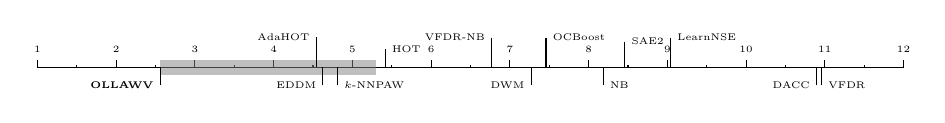
\begin{tikzpicture}
\draw (1,0) -- (12,0);
\foreach \x in {1,2,3,4,5,6,7,8,9,10,11,12} {
\draw (\x, 0) -- ++(0,.1) node [above,scale=0.7] {\tiny \x};
\ifthenelse{\x < 12}{\draw (\x+.5, 0) -- ++(0,.03);}{}
}

\coordinate (c0) at (2.5625,0);
\coordinate (c1) at (5.4167,0);
\coordinate (c2) at (4.5417,0);
\coordinate (c3) at (8.1875,0);
\coordinate (c4) at (4.8125,0);
\coordinate (c5) at (4.625,0);
\coordinate (c6) at (10.9583,0);
\coordinate (c7) at (6.7708,0);
\coordinate (c8) at (8.4583,0);
\coordinate (c9) at (9.0417,0);
\coordinate (c10) at (7.2708,0);
\coordinate (c11) at (10.8958,0);
\coordinate (c12) at (7.4583,0);

\node (l0) at (c0) [below left=.1cm and 0cm, align=right,scale=0.7] {\tiny \textbf{OLLAWV}};
\node (l1) at (c1) [above right=.1cm and 0cm, align=right,scale=0.7] {\tiny HOT};
\node (l2) at (c2) [above left=.25cm and 0cm, align=right,scale=0.7] {\tiny AdaHOT};
\node (l3) at (c3) [below right=.1cm and 0cm, align=right,scale=0.7] {\tiny NB};
\node (l4) at (c4) [below right=.1cm and 0cm, align=right,scale=0.7] {\tiny $k$-NNPAW};
\node (l5) at (c5) [below left=.1cm and 0cm, align=right,scale=0.7] {\tiny EDDM};
\node (l6) at (c6) [below right=.1cm and 0cm, align=right,scale=0.7] {\tiny VFDR};
\node (l7) at (c7) [above left=.25cm and 0cm, align=right,scale=0.7] {\tiny VFDR-NB};
\node (l8) at (c8) [above right=.2cm and 0cm, align=right,scale=0.7] {\tiny SAE2};
\node (l9) at (c9) [above right=.25cm and 0cm, align=right,scale=0.7] {\tiny LearnNSE};
\node (l10) at (c10) [below left=.1cm and 0cm, align=right,scale=0.7] {\tiny DWM};
\node (l11) at (c11) [below left=.1cm and 0cm, align=right,scale=0.7] {\tiny DACC};
\node (l12) at (c12) [above right=.25cm and 0cm, align=right,scale=0.7] {\tiny OCBoost};

\fill[fill=gray,fill opacity=0.5] (2.5625,-0.1) rectangle (5.3,0.1);

\foreach \x in {0,1,2,3,4,5,6,7,8,9,10,11,12} {
\draw (l\x) -| (c\x);
};
\end{tikzpicture}}\vspace{-1em}
\captionsetup{width=\linewidth}
\captionof{figure}{Bonferroni-Dunn test for Accuracy}\label{fig:BonfDunnaccDS}
\end{minipage}
\end{table}
\subsection{Accuracy}
% CD for 0.05 alpha is 2.789
Table~\ref{tab:DSResultsacc} shows the accuracy results of the 13 algorithms over 24 data streams along with their average and rank. %The results indicate that classifiers that used a passive approach to concept drift performed better overall than those that utilized an active change-detector.
Specifically, OLLAWV achieves the best accuracy over 19 of the 24 datasets, with a competitive average against $k$-NNwPAW and AdaHOT. Note that OLLAWV performs competitively with the algorithms that employ a change-detector on faster drifting streams. Friedman statistic (distributed according to chi-square with 12 degrees of freedom): 122.7239

Figure~\ref{fig:BonfDunnaccDS} show the results for the statistical analysis on the accuracy results. The algorithms with rank higher than $4.99$ (OLLAWV rank + Bonferroni-Dunn critical value), to the right of the gray bar in Figure~\ref{fig:BonfDunnaccDS}, perform statistically worse than OLLAWV. 


\begin{table}[b!]
\caption{Cohen's Kappa (\%) Comparison for Data Stream Classifiers}
\scriptsize
\centering
\label{tab:DSResultskappa}
\resizebox{\textwidth}{!}{\begin{tabularx}{1.55\textwidth}{l@{\extracolsep{\fill}}ccccccccccccccc}
\noalign{\smallskip}\hline\noalign{\smallskip}
Dataset & OLLAWV & HOT & AdaHOT & NB & $k$-NNPAW & EDDM & VFDR & VFDRNB & SAE2 & LearnNSE &DWM &DACC &OCBoost &\\
\noalign{\smallskip}\hline\noalign{\smallskip}
CovType &\textbf{84.2997} &76.4406 &77.6946 &40.1567 &80.4264 &34.1059 &31.4704 &61.1629 &62.9842 &50.6291 &55.5296 &36.6365 &48.2357 &  \\
census &5.0601 &34.3735 &\textbf{37.3923} &35.9631 &22.1060 &20.3869 &6.9733 &18.9029 &18.6604 &17.4783 &36.1846 &16.6752 &33.6569 &  \\
shuttle &96.1715 &94.9072 &95.8499 &75.0367 &\textbf{97.9178} &95.7487 &60.8151 &89.5257 &75.3213 &81.5605 &75.1038 &74.9782 &36.6910 &  \\
RBFNoDrift &\textbf{88.4224} &85.8825 &85.9195 &43.9848 &87.4934 &84.9571 &55.0695 &63.4111 &78.3215 &40.5704 &40.8376 &30.0155 &84.1671 &  \\
LEDNoDrift &70.9202 &70.9448 &70.9273 &\textbf{71.0466} &62.0311 &70.7085 &34.6226 &70.8356 &63.9960 &64.2672 &67.9406 &42.5203 &8.2749 &  \\
HyperplaneSlow &\textbf{80.1826} &64.1930 &64.8410 &55.3808 &68.0514 &63.1314 &37.7662 &70.3768 &66.9693 &72.4088 &76.1199 &61.3233 &71.5516 &  \\
HyperplaneFaster &\textbf{79.0184} &65.4333 &70.6839 &54.4616 &68.5439 &68.6522 &57.2656 &70.3619 &67.6281 &72.9982 &73.5220 &62.3085 &75.5906 &  \\
RBFGradualRecurring &97.8807 &92.8205 &92.5769 &44.2773 &\textbf{97.8977} &91.2740 &46.6574 &81.5090 &84.6106 &63.7269 &66.5421 &49.0047 &31.4648 &  \\
RBFBlips &\textbf{98.7358} &94.1422 &94.0557 &46.9730 &98.5651 &93.1254 &55.0797 &84.2691 &85.2017 &69.5671 &72.8462 &56.9876 &32.7263 &  \\
WaveformGenerator &75.9070 &74.4807 &\textbf{76.2084} &70.6198 &70.1883 &75.4134 &45.8181 &63.7626 &70.2764 &70.2900 &67.5944 &60.3864 &32.6201 &  \\
STAGGERGeneratorF1 &\textbf{100.0000} &99.9429 &99.9429 &\textbf{100.0000} &\textbf{100.0000} &\textbf{100.0000} &99.5649 &\textbf{100.0000} &78.2768 &14.6120 &\textbf{100.0000} &99.7795 &\textbf{100.0000} &  \\
HyperplaneFaster0.2 &\textbf{78.9822} &65.5488 &70.7205 &54.5039 &68.5467 &75.2763 &57.7700 &70.2251 &67.6807 &73.0150 &73.5124 &62.4578 &75.1728 &  \\
RBFGradualRecurringv2 &\textbf{96.2323} &91.0414 &90.6582 &43.1602 &94.3039 &90.9059 &43.9448 &74.2539 &79.2448 &49.7920 &51.6529 &32.3653 &30.8075 &  \\
MixedGeneratorBT &95.9938 &98.2128 &\textbf{98.6438} &83.8667 &95.3299 &98.2134 &66.2440 &86.5611 &86.3155 &81.8128 &82.3886 &78.3117 &97.9588 &  \\
MixedGeneratorBF &96.0417 &98.3495 &\textbf{98.7154} &83.9979 &95.1582 &98.4008 &79.8200 &88.5565 &86.7861 &81.4176 &82.8106 &77.0956 &97.8810 &  \\
RandomRBFGeneratorC4A25 &\textbf{98.8172} &96.5331 &96.1343 &75.2231 &98.2308 &95.7997 &62.3923 &85.1851 &87.3386 &70.6112 &72.5571 &49.6768 &36.2515 &  \\
RandomRBFGeneratorC4A50 &\textbf{99.6519} &98.8615 &98.8319 &89.0625 &98.8693 &98.6371 &73.7051 &94.0710 &89.1866 &81.1006 &87.0871 &64.3007 &35.4000 &  \\
SineGeneratorF1BF &95.5500 &\textbf{99.4950} &99.4517 &86.9837 &91.0397 &99.3224 &89.5374 &91.7509 &88.9544 &84.9693 &86.4903 &84.2484 &99.0107 &  \\
SineGeneratoF2BF &95.5500 &\textbf{99.4896} &99.4493 &86.9837 &90.7381 &99.3195 &90.4504 &92.1487 &89.0741 &84.9693 &86.5495 &84.2484 &98.9512 &  \\
STAGGERGeneratorF1BF &\textbf{100.0000} &99.9429 &99.9429 &\textbf{100.0000} &\textbf{100.0000} &\textbf{100.0000} &99.5649 &\textbf{100.0000} &78.2768 &14.6120 &\textbf{100.0000} &99.7795 &\textbf{100.0000} &  \\
STAGGERGeneratorF2BF &\textbf{100.0000} &99.9542 &99.9542 &\textbf{100.0000} &\textbf{100.0000} &99.9542 &99.7331 &\textbf{100.0000} &89.9239 &0.0000 &\textbf{100.0000} &\textbf{100.0000} &-96.4666 &  \\
HyperplaneFasterAN5 &\textbf{78.5796} &65.3782 &70.4883 &74.7517 &68.3699 &77.4733 &58.2704 &69.7705 &67.4541 &72.8100 &73.3486 &62.2368 &74.7517 &  \\
SEASuddenAN0 &73.8014 &67.6140 &68.1883 &74.8009 &72.7554 &\textbf{76.3943} &59.8618 &68.0628 &68.2933 &69.2729 &72.0454 &64.9863 &74.8009 &  \\
SEASuddenAN05 &73.1889 &66.8436 &67.4079 &73.2812 &72.2042 &\textbf{74.9242} &59.9057 &67.9381 &67.1285 &68.9706 &71.2053 &64.5598 &73.2812 &  \\
\noalign{\smallskip}\hline\noalign{\smallskip}
Average &\textbf{85.7911} &83.3677 &84.3616 &69.3548 &83.2820 &82.5885 &61.3460 &77.6101 &74.9127 &60.4776 &73.8278 &63.1201 &56.3658 &  \\
Rank &\textbf{3.0208} &5.5417 &4.5833 &7.7500 &4.8542 &4.5833 &11.3750 &6.6042 &8.2500 &8.9167 &6.9375 &11.1458 &7.4375 &  \\
\noalign{\smallskip}\hline\noalign{\smallskip}
\end{tabularx}}
\begin{minipage}{0.9\textwidth}
\centering
\resizebox{\textwidth}{!}{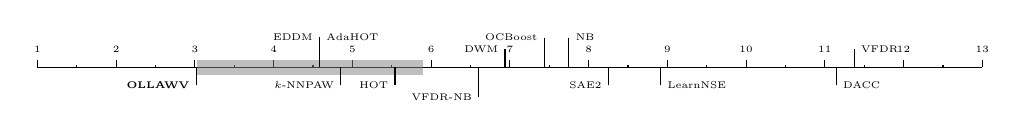
\begin{tikzpicture}
\draw (1,0) -- (13,0);
\foreach \x in {1,2,3,4,5,6,7,8,9,10,11,12,13} {
\draw (\x, 0) -- ++(0,.1) node [above,scale=0.7] {\tiny \x};
\ifthenelse{\x < 13}{\draw (\x+.5, 0) -- ++(0,.03);}{}
}

\coordinate (c0) at (3.0208,0);
\coordinate (c1) at (5.5417,0);
\coordinate (c2) at (4.5833,0);
\coordinate (c3) at (7.75,0);
\coordinate (c4) at (4.8542,0);
\coordinate (c5) at (4.5833,0);
\coordinate (c6) at (11.375,0);
\coordinate (c7) at (6.6042,0);
\coordinate (c8) at (8.25,0);
\coordinate (c9) at (8.9167,0);
\coordinate (c10) at (6.9375,0);
\coordinate (c11) at (11.1458,0);
\coordinate (c12) at (7.4375,0);

\node (l0) at (c0) [below left=.1cm and 0cm, align=right,scale=0.7] {\tiny \textbf{OLLAWV}};
\node (l1) at (c1) [below left=.1cm and 0cm, align=right,scale=0.7] {\tiny HOT};
\node (l2) at (c2) [above right=.25cm and 0cm, align=right,scale=0.7] {\tiny AdaHOT};
\node (l3) at (c3) [above right=.25cm and 0cm, align=right,scale=0.7] {\tiny NB};
\node (l4) at (c4) [below left=.1cm and 0cm, align=right,scale=0.7] {\tiny $k$-NNPAW};
\node (l5) at (c5) [above left=.25cm and 0cm, align=right,scale=0.7] {\tiny EDDM};
\node (l6) at (c6) [above right=.1cm and 0cm, align=right,scale=0.7] {\tiny VFDR};
\node (l7) at (c7) [below left=.25cm and 0cm, align=right,scale=0.7] {\tiny VFDR-NB};
\node (l8) at (c8) [below left=.1cm and 0cm, align=right,scale=0.7] {\tiny SAE2};
\node (l9) at (c9) [below right=.1cm and 0cm, align=right,scale=0.7] {\tiny LearnNSE};
\node (l10) at (c10) [above left=.1cm and 0cm, align=right,scale=0.7] {\tiny DWM};
\node (l11) at (c11) [below right=.1cm and 0cm, align=right,scale=0.7] {\tiny DACC};
\node (l12) at (c12) [above left=.25cm and 0cm, align=right,scale=0.7] {\tiny OCBoost};

\fill[fill=gray,fill opacity=0.5] (3.0208,-0.1) rectangle (5.9,0.1);

\foreach \x in {0,1,2,3,4,5,6,7,8,9,10,11,12} {
\draw (l\x) -| (c\x);
};
\end{tikzpicture}}\vspace{-1em}
\captionsetup{width=\linewidth}
\captionof{figure}{Bonferroni-Dunn test for Cohen's Kappa}\label{fig:BonfDunnkappaDS}
\end{minipage}
\end{table}
\subsection{Cohen's Kappa Rate}
Table~\ref{tab:DSResultskappa} shows the Cohen's Kappa rate results obtained by the algorithms. These results complement the accuracy results achieved by the algorithms, in the sense that... OLLAWV's kappa values all fall within the ($50\%$, $100\%$] range, with the exception of the census dataset, indicating that its merit as a classifier agrees with the class distribution, and is not random. Concerning the census dataset, the best result, achieved by AdaHOT, was $37.3923\%$, meaning all algorithms performed approximately randomly. Classifiers OCBoost, DACC, Learn++.NSE, and VFDR all achieved the lowest rates on average. Note, Learn++.NSE obtained a 0, indicating complete random classifier behavior.

\subsection{Training Time}
\begin{table}[t!]
\caption{Training Time (seconds) Comparison for Data Stream Classifiers}
\scriptsize
\centering
\label{tab:DSResultsTrain}
\resizebox{\textwidth}{!}{\begin{tabularx}{1.55\textwidth}{l@{\extracolsep{\fill}}ccccccccccccccc}
\noalign{\smallskip}\hline\noalign{\smallskip}
Dataset & OLLAWV & HOT & AdaHOT & NB & $k$-NNPAW & EDDM & VFDR & VFDR-NB & SAE2 & LearnNSE &DWM &DACC &OCBoost &\\
\noalign{\smallskip}\hline\noalign{\smallskip}
CovType &0.0451 &0.0765 &0.0909 &\textbf{0.0009} &0.0387 &0.0577 &0.0371 &0.0445 &0.1121 &6.2806 &0.0419 &0.0357 &0.0984 &  \\
census &0.0168 &0.1040 &0.1162 &\textbf{0.0007} &0.0386 &0.0345 &0.0735 &0.0458 &0.0363 &0.9368 &0.0156 &0.0175 &0.0543 &  \\
shuttle &0.0103 &0.0276 &0.0298 &\textbf{0.0004} &0.0386 &0.0069 &0.0108 &0.0069 &0.0217 &0.2692 &0.0104 &0.0186 &0.0581 &  \\
RBFNoDrift &0.0329 &0.0174 &0.0247 &\textbf{0.0002} &0.0383 &0.0828 &0.4267 &0.3172 &0.0491 &3.4029 &0.0104 &0.0137 &0.0402 &  \\
LEDNoDrift &0.0697 &0.0373 &0.0649 &\textbf{0.0003} &0.0389 &0.0245 &0.0097 &0.0082 &0.0694 &5.4734 &0.0175 &0.0290 &0.0547 &  \\
HyperplaneSlow &0.0353 &0.0094 &0.0142 &\textbf{0.0002} &0.0389 &0.1405 &0.1871 &0.3006 &0.0473 &3.3734 &0.0091 &0.0142 &0.0389 &  \\
HyperplaneFaster &0.0263 &0.0295 &0.0416 &\textbf{0.0002} &0.0384 &0.1231 &0.3016 &0.3784 &0.0424 &3.2991 &0.0098 &0.0143 &0.0376 &  \\
RBFGradualRecurring &0.0456 &0.0316 &0.0369 &\textbf{0.0003} &0.0389 &0.0391 &1.1284 &0.9295 &0.1004 &11.7980 &0.0335 &0.0474 &0.1070 &  \\
RBFBlips &0.0396 &0.0243 &0.0299 &\textbf{0.0003} &0.0384 &0.0278 &0.7587 &0.8342 &0.0948 &11.9934 &0.0342 &0.0473 &0.1050 &  \\
WaveformGenerator &0.0394 &0.0751 &0.0965 &\textbf{0.0006} &0.0390 &0.1847 &0.9670 &0.9271 &0.1715 &17.9675 &0.0511 &0.0743 &0.1318 &  \\
STAGGERGeneratorF1 &0.0021 &0.0006 &0.0007 &\textbf{0.0001} &0.0389 &0.0005 &0.0013 &0.0007 &0.0018 &0.5517 &0.0003 &0.0020 &0.0113 &  \\
HyperplaneFaster0.2 &0.0268 &0.0302 &0.0465 &\textbf{0.0002} &0.0388 &0.0260 &0.3192 &0.3010 &0.0456 &3.2893 &0.0095 &0.0141 &0.0372 &  \\
RBFGradualRecurringv2 &0.0545 &0.0169 &0.0203 &\textbf{0.0003} &0.0383 &0.0859 &0.7622 &0.7634 &0.0552 &12.0529 &0.0367 &0.0464 &0.1053 &  \\
MixedGeneratorBT &0.0205 &0.0027 &0.0026 &\textbf{0.0001} &0.0336 &0.0071 &1.7640 &1.5534 &0.0086 &0.9761 &0.0024 &0.0052 &0.0204 &  \\
MixedGeneratorBF &0.0299 &0.0024 &0.0024 &\textbf{0.0001} &0.0334 &0.0065 &1.1035 &1.0924 &0.0093 &0.8971 &0.0024 &0.0058 &0.0209 &  \\
RandomRBFGeneratorC4A25 &0.0200 &0.0441 &0.0407 &\textbf{0.0003} &0.0358 &0.0730 &1.7831 &1.6927 &0.1245 &13.9876 &0.0395 &0.0719 &0.1580 &  \\
RandomRBFGeneratorC4A50 &0.0157 &0.0333 &0.0337 &\textbf{0.0007} &0.0350 &0.0909 &2.8802 &2.5559 &0.1917 &27.8456 &0.0752 &0.1432 &0.2974 &  \\
SineGeneratorF1BF &0.0122 &0.0056 &0.0056 &\textbf{0.0001} &0.0334 &0.0073 &1.9301 &2.9169 &0.0127 &1.3768 &0.0034 &0.0071 &0.0235 &  \\
SineGeneratoF2BF &0.0121 &0.0051 &0.0053 &\textbf{0.0001} &0.0314 &0.0077 &5.0598 &5.9477 &0.0117 &1.3996 &0.0027 &0.0074 &0.0236 &  \\
STAGGERGeneratorF1BF &0.0021 &0.0006 &0.0006 &\textbf{0.0001} &0.0323 &0.0005 &0.0006 &0.0005 &0.0015 &0.6175 &0.0003 &0.0022 &0.0143 &  \\
STAGGERGeneratorF2BF &0.0022 &0.0010 &0.0009 &\textbf{0.0001} &0.0340 &0.0006 &0.0005 &0.0005 &0.0017 &0.6752 &0.0003 &0.0020 &0.0139 &  \\
HyperplaneFasterAN5 &0.0264 &0.0200 &0.0200 &0.0440 &0.0269 &0.0115 &0.2298 &0.2417 &0.0312 &2.5014 &\textbf{0.0080} &0.0147 &0.0740 &  \\
SEASuddenAN0 &0.0208 &0.0051 &0.0052 &0.0268 &0.0312 &0.0099 &0.0370 &0.0373 &0.0176 &1.3545 &\textbf{0.0032} &0.0059 &0.0335 &  \\
SEASuddenAN05 &0.0284 &0.0055 &0.0055 &0.0257 &0.0309 &0.0095 &0.0321 &0.0334 &0.0167 &1.3365 &\textbf{0.0032} &0.0061 &0.0326 &  \\
\noalign{\smallskip}\hline\noalign{\smallskip}
Average &0.0264 &0.0252 &0.0307 &\textbf{0.0043} &0.0359 &0.0441 &0.8252 &0.8721 &0.0531 &5.5690 &0.0175 &0.0269 &0.0663 &  \\
Rank &6.5833 &4.7917 &5.7917 &\textbf{1.8750} &7.7500 &6.0833 &9.8333 &9.5833 &8.2917 &12.6667 &2.7917 &5.5417 &9.4167 &  \\
\noalign{\smallskip}\hline\noalign{\smallskip}
\end{tabularx}}
\begin{minipage}{0.9\textwidth}
\centering
\resizebox{\textwidth}{!}{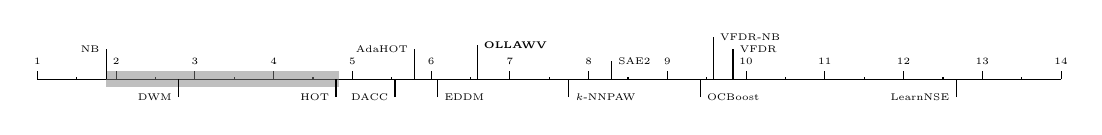
\begin{tikzpicture}
\draw (1,0) -- (14,0);
\foreach \x in {1,2,3,4,5,6,7,8,9,10,11,12,13,14} {
\draw (\x, 0) -- ++(0,.1) node [above,scale=0.7] {\tiny \x};
\ifthenelse{\x < 14}{\draw (\x+.5, 0) -- ++(0,.03);}{}
}

\coordinate (c0) at (6.5833,0);
\coordinate (c1) at (4.7917,0);
\coordinate (c2) at (5.7917,0);
\coordinate (c3) at (1.875,0);
\coordinate (c4) at (7.75,0);
\coordinate (c5) at (6.0833,0);
\coordinate (c6) at (9.8333,0);
\coordinate (c7) at (9.5833,0);
\coordinate (c8) at (8.2917,0);
\coordinate (c9) at (12.6667,0);
\coordinate (c10) at (2.7917,0);
\coordinate (c11) at (5.5417,0);
\coordinate (c12) at (9.4167,0);

\node (l0) at (c0) [above right=.3cm and 0cm, align=right,scale=0.7] {\tiny \textbf{OLLAWV}};
\node (l1) at (c1) [below left=.1cm and 0cm, align=right,scale=0.7] {\tiny HOT};
\node (l2) at (c2) [above left=.25cm and 0cm, align=right,scale=0.7] {\tiny AdaHOT};
\node (l3) at (c3) [above left=.25cm and 0cm, align=right,scale=0.7] {\tiny NB};
\node (l4) at (c4) [below right=.1cm and 0cm, align=right,scale=0.7] {\tiny $k$-NNPAW};
\node (l5) at (c5) [below right=.1cm and 0cm, align=right,scale=0.7] {\tiny EDDM};
\node (l6) at (c6) [above right=.25cm and 0cm, align=right,scale=0.7] {\tiny VFDR};
\node (l7) at (c7) [above right=.4cm and 0cm, align=right,scale=0.7] {\tiny VFDR-NB};
\node (l8) at (c8) [above right=.1cm and 0cm, align=right,scale=0.7] {\tiny SAE2};
\node (l9) at (c9) [below left=.1cm and 0cm, align=right,scale=0.7] {\tiny LearnNSE};
\node (l10) at (c10) [below left=.1cm and 0cm, align=right,scale=0.7] {\tiny DWM};
\node (l11) at (c11) [below left=.1cm and 0cm, align=right,scale=0.7] {\tiny DACC};
\node (l12) at (c12) [below right=.1cm and 0cm, align=right,scale=0.7] {\tiny OCBoost};

\fill[fill=gray,fill opacity=0.5] (1.875,-0.1) rectangle (4.835,0.1);

\foreach \x in {0,1,2,3,4,5,6,7,8,9,10,11,12} {
\draw (l\x) -| (c\x);
};
\end{tikzpicture}}\vspace{-1em}
\captionsetup{width=\linewidth}
\captionof{figure}{Bonferroni-Dunn test for Training Time}\label{fig:BonfDunnTrainDS}
\end{minipage}
\end{table}


\subsection{Overall Comparison}


\section{Conclusions}

\chapter{Conclusions}
This thesis introduced several novel SVM algorithms for learning from the following diverse learning paradigms: multi-target regression, multi-instance classification, data stream classification, and traditional supervised classification.

Three unique approaches for multi-target regression were proposed: the baseline problem transformation support vector regressor SVR, an ensemble of randomly generated chains using this base model SVRRC, and a maximally correlated chained model SVRCC. The results highlighted the better performance of SVR as a base model, however, because it is a problem transformation method, the possible correlations amongst the targets are lost on the final model. SVRRC was designed to test whether taking these correlations into account would benefit the final learning model, and the results showed a performance increase. However, due to the random nature of SVRRC, capturing target correlations is not guaranteed. SVRCC was designed to remedy this issue using a maximum correlation chain and proved to capture target correlations accurately, providing the best results among the contributions, as well as against the methods compared. 

A novel multiple-instance bag-level formulation and algorithm, dubbed MIRSVM, with a bag-representative selector, are proposed. The algorithm trains the SVM on bag-level information, iteratively selecting the best representative instance for each positive and negative bag, while finding the optimal separating hyperplane. This approach, unlike other existing ones, eliminates possible class imbalance issues by allowing both positive and negative bags to be represented. The experimental and statistical study showed that bag-level learners outperform instance-level learners and wrapper methods. MIRSVM outperformed current contemporary SVM multi-instance algorithms, as well as other algorithms of different classes over several metrics.

After the previous experimental studies, it was evident that the existing popular SVM solvers that were used suffered from several disadvantages when used in traditional and non-traditional settings. This prompted the design and implementation of a novel online, also known as stochastic, learning algorithm for solving the L1-SVM problem, dubbed OLLAWV. Unlike other online methods, OLLAWV eliminates the need for specifying the number of iterations, as well as the use of a regularization term. The proposed algorithm uses early stopping as its regularizer. OLLAWV also was designed to have a novel stopping criteria, a trait that most stochastic methods do not have. The experimental study, involving strict nested cross-validation, evaluated and compared the proposal with current popular SVM kernel methods that have been shown to outperform the traditional and widely used approaches for solving L1-SVMs, such as SMO and quadratic programming solvers. The results of the experimental study, along with complementary statistical analysis, showed the better performance of OLLAWV against the compared methods, along with 5 non-SVM contemporary methods. OLLAWV was shown to produce sparse models at very fast speeds, without sacrificing accuracy. This, along with the online nature of OLLAWV, prompted the investigation of its performance in the data stream setting. 

The final contribution of this thesis involved implementing OLLAWV in a batch data stream classification setting. 

\chapter{Future Work}
The contributions proposed in this thesis have a few paths to follow in terms of future work:
\begin{enumerate}
\item The first option could be to extend OLLAWV to the regression case. 
\item If OLLAWV is extended to the regression case, it can be applied to the Multi-Target Regression paradigm. It could be used instead of the SMO algorithm in the proposed implementations in Chapter~\ref{chap:mtr}. 
\item OLLAWV could also be implemented within the Multi-Instance Classification contribution, rather than using the quadratic programming solver. 
\item To further improve the performance of OLLAWV, another line of investigation would be experimenting with a parallelized/distributed implementation.
\item Finally, in the context of data stream classification, a non-batch version of OLLAWV could be investigated.
\end{enumerate}

\printbibliography[title={References}, heading=bibintoc]

\begin{comment}

\begin{appendices}
\titleformat{\chapter}[display]{\bfseries\centering}{\huge Appendix \thechapter}{1em}{\Huge #1}
\chapter{Publications}
\newpage
% MIRSVM
\thispagestyle{plain}
\begin{center}
    \vspace*{0.5 cm}
     \textsc{\LARGE MIRSVM: Multi-Instance SVM using Bag Representatives}\\[0.5 cm]
     \textsc{\textit{Authors: }Gabriella Melki, Alberto Cano, Sebastian Ventura}\\[0.5 cm]		
     
     
\includegraphics[scale = 0.25]{figures/pr.jpg}\\[0.5 cm]	
     \textsc{Pattern Recognition, Volume 79, pp. 228-241, July 2018}\\[0.5 cm]		
	
	\begin{minipage}{0.6\textwidth}
	\centering
		\textsc{Publisher: Elsevier}\\
	    	\textsc{Impact Factor: 4.582}\\
	    	\textsc{DOI:} 10.1016/j.patcog.2018.02.007 \\
	\end{minipage}\\[2 cm]
\end{center}
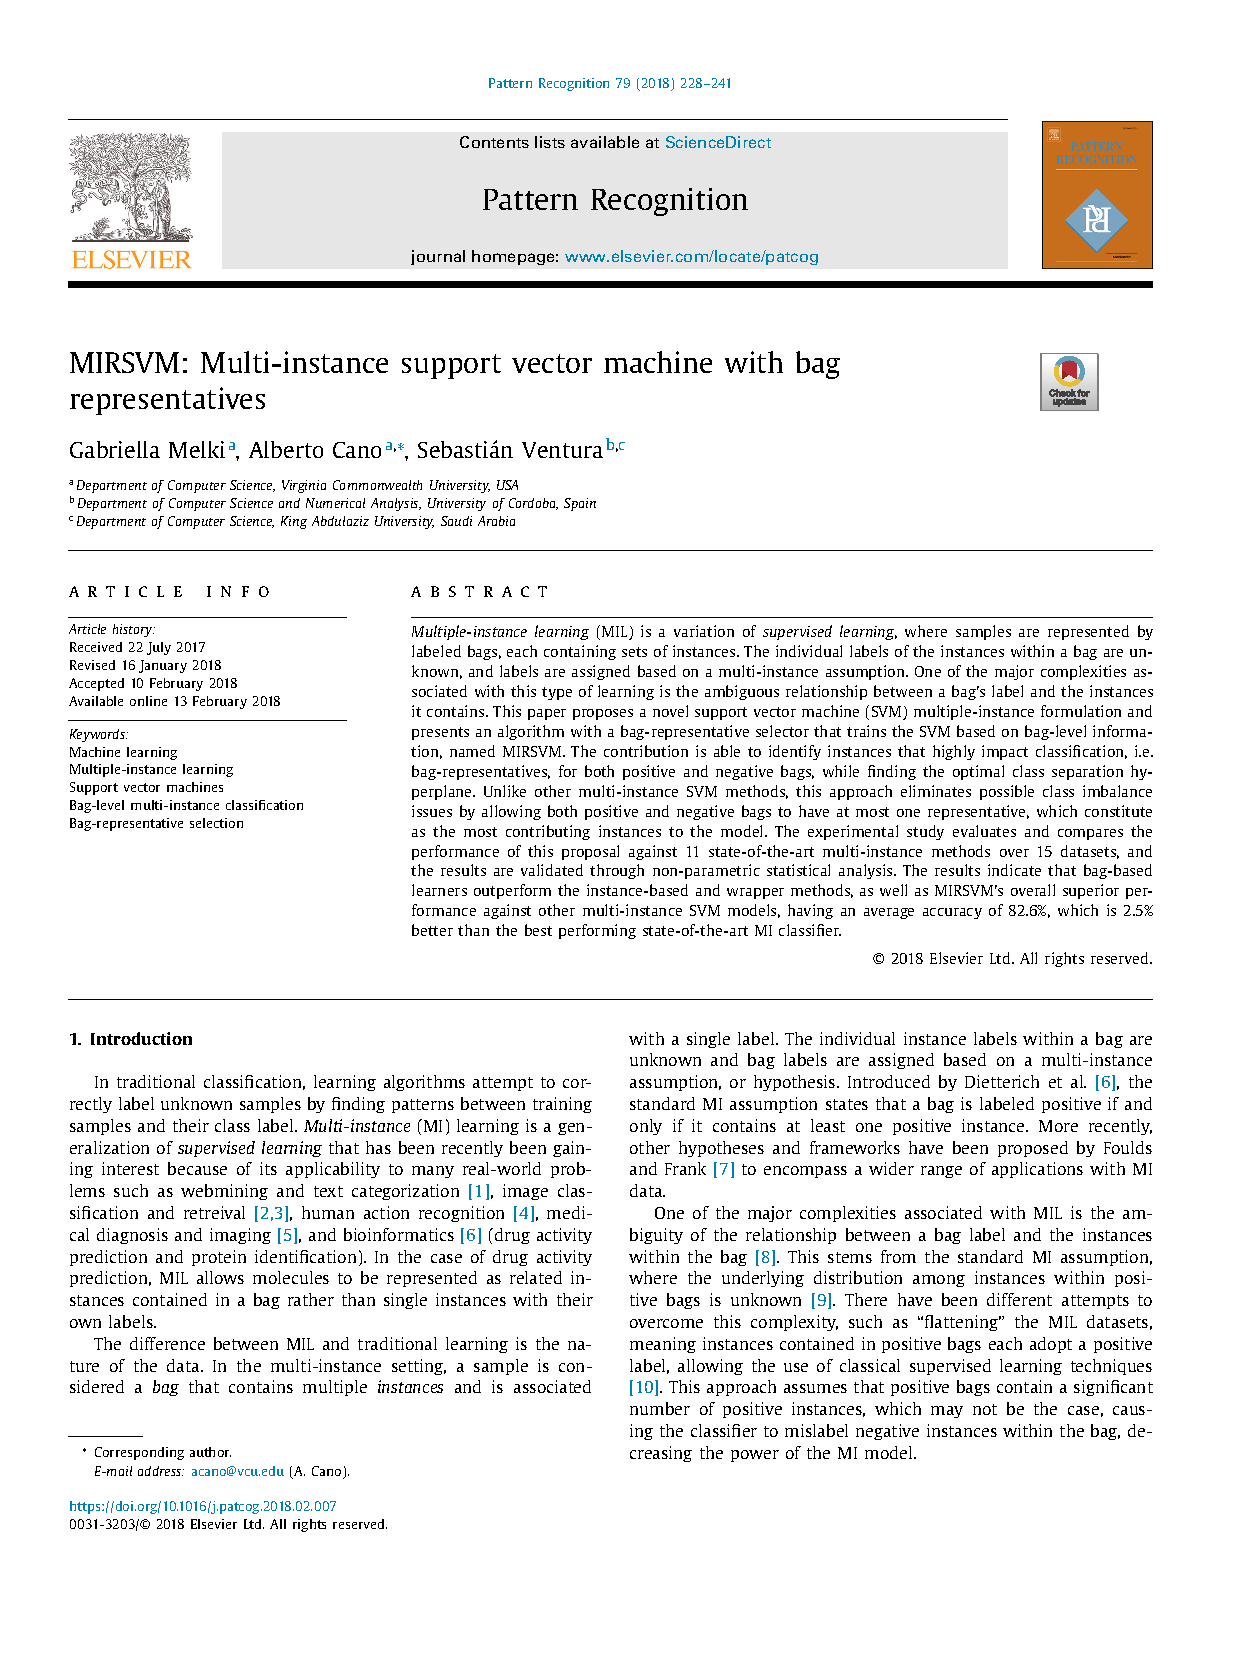
\includepdf[pages=1,pagecommand=\section{MIRSVM: Multi-Instance SVM with Bag Representatives},scale=.8,linktodoc=true]{publications/mirsvm.pdf}
\includepdf[pages={2-},scale=.8,linktodoc=true]{publications/mirsvm.pdf}


% MULTI_TARGET
\begin{center}
    \vspace*{0.5 cm}
     \textsc{\LARGE Multi-Target Support Vector Regression Via Correlation Regressor Chains}\\[0.5 cm]
     \textsc{\textit{Authors: }Gabriella Melki, Alberto Cano, Vojislav Kecman, Sebastian Ventura}\\[0.5 cm]		
     
     
\includegraphics[scale = 0.25]{figures/is.jpg}\\[0.5 cm]	
     \textsc{Information Sciences, Volumes 415–-416, pp. 53-69, November 2017}\\[0.5 cm]	
	
	\begin{minipage}{0.6\textwidth}
	\centering
		\textsc{Publisher: Elsevier}\\
	    	\textsc{Impact Factor: 4.832}\\
	    	\textsc{DOI:} 10.1016/j.ins.2017.06.017 \\
	\end{minipage}\\[2 cm]
\end{center}
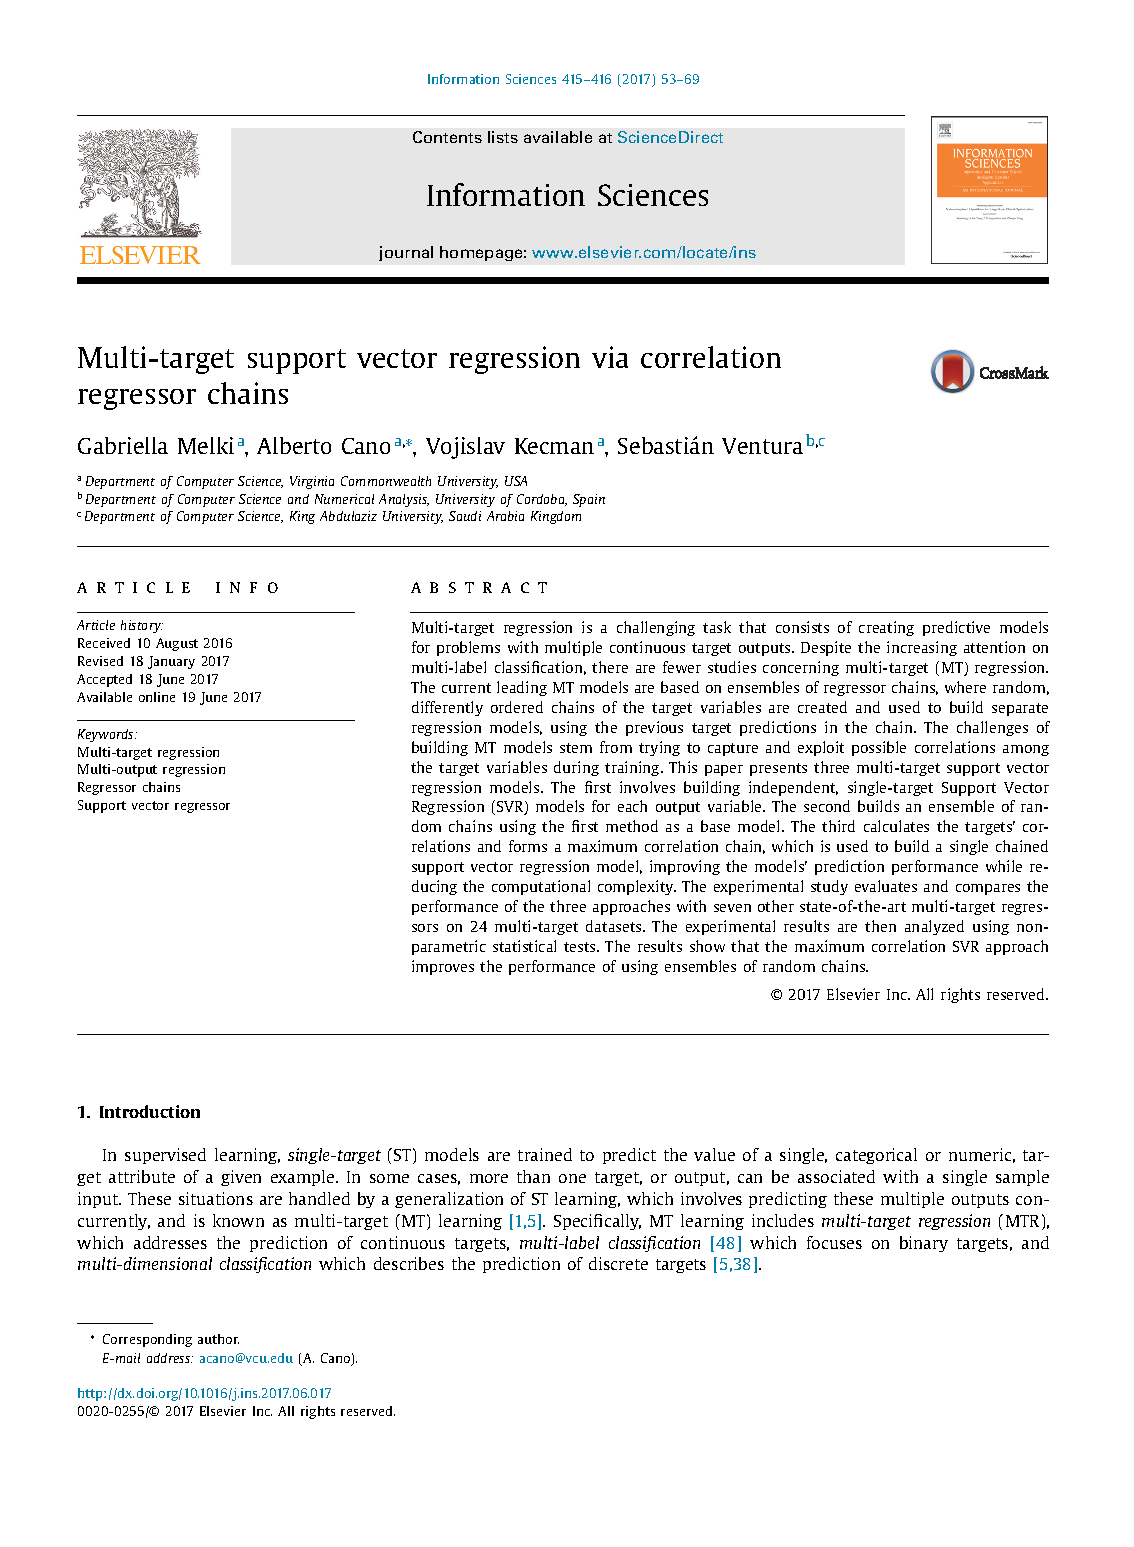
\includepdf[pages=1,pagecommand=\section{Multi-Target Support Vector Regression Via Correlation Regressor Chains},scale=.8,linktodoc=true]{publications/mtr.pdf}
\includepdf[pages={2-},scale=.8,linktodoc=true]{publications/mtr.pdf}

% ACRONYMS
\chapter{List of Acronyms}
\begin{longtable}{ p{.20\textwidth}  p{.80\textwidth} } 
\textbf{aCC} & Average Correlation Coefficient \\
\textbf{APR} & Axis Parallel Rectangle \\
\textbf{aRMSE} & Average Root Mean Squared Error \\
\textbf{aRRMSE} & Average Relative Root Mean Squared Error \\
\textbf{AUC} & Area Under ROC Curve \\
\textbf{BVM} & Ball Vector Machines \\
\textbf{CitationKNN} & Citation k-Nearest Neighbors \\
\textbf{CV} & Cross Validation \\
\textbf{CVM} & Core Vector Machines \\
\textbf{DD} & Diverse Density \\
\textbf{EM-DD} & Expectation-Maximization Diverse Density \\
\textbf{ERC} & Ensemble of Random Chains \\
\textbf{ERCC} & Ensemble of Random Chains Corrected \\
\textbf{FN} & False Negative \\
\textbf{FP} & False Positive \\
\textbf{ISDA} & Iterative Single Data Algorithm \\
\textbf{$k$-NN} & $k$-Nearest Neighbors \\
\textbf{MI} & Multiple Instance \\
\textbf{miGraph} & Mixed Integer Graph \\
\textbf{MIL} & Multiple Instance Learning \\
\textbf{MIOptimalBall} & Multiple Instance Optimal Ball \\
\textbf{MIRI} & Multi-Instance Rule Induction \\
\textbf{MIRSVM} & Multi-Instance Support Vector Machine \\
\textbf{MISMO} & Multiple Instance Sequential Minimal Optimization \\
\textbf{MITI} & Multi-Instance Tree Inducer \\
\textbf{MNSVM} & Minimal Norm Support Vector Machine \\
\textbf{MORF} & Multi-Objective Random Forests \\
\textbf{MSE} & Mean Squared Error \\
\textbf{MT} & Multiple Target \\
\textbf{MTR} & Multiple Target Regression \\
\textbf{MTS} & Multiple Target Stacking \\
\textbf{MTSC} & Multiple Target Stacking Corrected \\
\textbf{NLSVR} & Non-Linear Support Vector Regressor \\
\textbf{NNISDA} & Non-Negative Iterative Single Data Algorithm \\
\textbf{NORMA} & "Na{\""}ve Online R Minimization Algorithm" \\
\textbf{OLLA} & Online Learning Algorithm \\
\textbf{PEGASOS} & Primal Estimated Sub-Gradient Solver for Support Vector Machines \\
\textbf{QP} & Quadratic Programming \\
\textbf{RC} & Random Chaining \\
\textbf{RCC} & Regression Chains Corrected \\
\textbf{ROC} & Receiver Operating Characteristic \\
\textbf{SGD} & Stochastic Gradient Descent \\
\textbf{SMI} & Standard Multiple Instance Assumption \\
\textbf{SMO} & Sequential Minimal Optimization \\
\textbf{SphereSVM} & Sphere Support Vector Machine \\
\textbf{SRM} & Structured Risk Minimization \\
\textbf{ST} & Single Target \\
\textbf{SVM} & Support Vector Machine \\
\textbf{SVR} & Support Vector Regressor \\
\textbf{SVRCC} & Support Vector Regressor with maximum Correlation Chaining \\
\textbf{SVRRC} & Support Vector Regressor with Random Chaining \\
\textbf{TLC} & Two-Level Classifier \\
\textbf{TN} & True Negative \\
\textbf{TP} & True Positive  \\
\end{longtable}

\end{appendices}

\end{comment}

\chapter*{Vita}
\thispagestyle{plain}
\addcontentsline{toc}{chapter}{Vita}
Gabriella Melki received her BSc. in Computer Science at the American University of Beirut in 2011 and her MSc. in Computer Science from Virginia Commonwealth University in 2016. As a full-time student in the dual Ph.D. program between Virginia Commonwealth University and the University of C\'{o}rdoba in Spain, her research is focused on machine learning algorithms for large datasets and various data paradigms. Her more specialized field of interest is support vector machines.

\textbf{Publications:}
\begin{itemize}
\item[-] \textbf{Melki G}, Kecman V, Ventura S, Cano A, ``OLLAWV: OnLine Learning using Worst-Violators", In: \textit{Applied Soft Computing} 66, (2018), pp. 384--393
\item[-] \textbf{Melki G}, Cano A, Ventura S, ``MIRSVM: Multi-Instance Support Vector Machine with Bag Representatives", In: \textit{Pattern Recognition} 75, (2018), pp. 228--214
\item[-] \textbf{Melki G}, Cano A, Kecman V, Ventura S, ``Multi-Target Support Vector Regression Via Correlation Regressor Chains", In: \textit{Information Sciences} 415, (2017), pp. 53--69
\item[-] \textbf{Melki G}, ``Fast Online Training of L1 Support Vector Machines", Master's Thesis, \textit{Virginia Commonwealth University}, (2016), pp. 1--64
\item[-] \textbf{Melki G}, Kecman V, ``Speeding Up Online Training of L1 Support Vector Machines", In: \textit{Proceedings of the IEEE SoutheastCon, 2016}, (2016), pp. 1--6
\item[-] Kecman V, \textbf{Melki G}, ``Fast Online Algorithm for SVMs", In: \textit{Proceedings of the IEEE SoutheastCon, 2016}. (2016), pp. 1--6
\item[-] Kecman V, Zigic L, \textbf{Melki G}, ``Models and Algorithms for Support Vector Machines: Direct L2 SVM'', \textit{Seminar at Max Planck Institute for Intelligent Systems, Empirical Inference}, T\"{u}bigen, Germany, 2015
\end{itemize}

\end{document}
